%&preformat-disser
\RequirePackage[l2tabu,orthodox]{nag} % Раскомментировав, можно в логе получать рекомендации относительно правильного использования пакетов и предупреждения об устаревших и нерекомендуемых пакетах
% Формат А4, 14pt (ГОСТ Р 7.0.11-2011, 5.3.6)
\documentclass[a4paper,14pt,oneside,openany]{memoir}

%%%%%%%%%%%%%%%%%%%%%%%%%%%%%%%%%%%%%%%%%%%%%%%%%%%%%%%%%%%%%%%%%%%%%%%%%%%%%%%%
%%%% Файл упрощённых настроек шаблона, общих для диссертации и автореферата %%%%
%%%%%%%%%%%%%%%%%%%%%%%%%%%%%%%%%%%%%%%%%%%%%%%%%%%%%%%%%%%%%%%%%%%%%%%%%%%%%%%%

%%% Режим черновика %%%
\makeatletter
\@ifundefined{c@draft}{
  \newcounter{draft}
  \setcounter{draft}{1}  % 0 --- чистовик (максимальное соблюдение ГОСТ)
                         % 1 --- черновик (отклонения от ГОСТ, но быстрая
                         %       сборка итоговых PDF)
}{}
\makeatother

%%% Пометки в тексте %%%
\makeatletter
\@ifundefined{c@showmarkup}{
  \newcounter{showmarkup}
  \setcounter{showmarkup}{0}  % 0 --- скрыть пометки
                              % 1 --- показывать пометки
}{}
\makeatother

%%% Использование в pdflatex шрифтов не по-умолчанию %%%
\makeatletter
\@ifundefined{c@usealtfont}{
  \newcounter{usealtfont}
  \setcounter{usealtfont}{1}    % 0 --- шрифты на базе Computer Modern
                                % 1 --- использовать пакет pscyr, при его
                                %       наличии
                                % 2 --- использовать пакет XCharter, при наличии
                                %       подходящей версии
}{}
\makeatother

%%% Использование в xelatex и lualatex семейств шрифтов %%%
\makeatletter
\@ifundefined{c@fontfamily}{
  \newcounter{fontfamily}
  \setcounter{fontfamily}{1}  % 0 --- CMU семейство. Используется как fallback;
                              % 1 --- Шрифты от MS (Times New Roman и компания)
                              % 2 --- Семейство Liberation
}{}
\makeatother

%%% Библиография %%%
\makeatletter
\@ifundefined{c@bibliosel}{
  \newcounter{bibliosel}
  \setcounter{bibliosel}{1}   % 0 --- встроенная реализация с загрузкой файла
                              %       через движок bibtex8;
                              % 1 --- реализация пакетом biblatex через движок
                              %       biber
}{}
\makeatother

%%% Вывод типов ссылок в библиографии %%%
\makeatletter
\@ifundefined{c@mediadisplay}{
  \newcounter{mediadisplay}
  \setcounter{mediadisplay}{1}   % 0 --- не делать ничего; надписи [Текст] и
                                 %       [Эл. ресурс] будут выводиться только в ссылках с
                                 %       заполненным полем `media`;
                                 % 1 --- автоматически добавлять надпись [Текст] к ссылкам с
                                 %       незаполненным полем `media`; таким образом, у всех
                                 %       источников будет указан тип, что соответствует
                                 %       требованиям ГОСТ
                                 % 2 --- автоматически удалять надписи [Текст], [Эл. Ресурс] и др.;
                                 %       не соответствует ГОСТ
                                 % 3 --- автоматически удалять надпись [Текст];
                                 %       не соответствует ГОСТ
                                 % 4 --- автоматически удалять надпись [Эл. Ресурс];
                                 %       не соответствует ГОСТ
}{}
\makeatother

%%% Предкомпиляция tikz рисунков для ускорения работы %%%
\makeatletter
\@ifundefined{c@imgprecompile}{
  \newcounter{imgprecompile}
  \setcounter{imgprecompile}{0}   % 0 --- без предкомпиляции;
                                  % 1 --- пользоваться предварительно
                                  %       скомпилированными pdf вместо генерации
                                  %       заново из tikz
}{}
\makeatother
            % общие настройки шаблона
\input{common/packages}         % Пакеты общие для диссертации и автореферата
\synopsisfalse                      % Этот документ --- не автореферат
\input{Dissertation/dispackages}    % Пакеты для диссертации
\input{Dissertation/userpackages}   % Пакеты для специфических пользовательских задач

%%%%%%%%%%%%%%%%%%%%%%%%%%%%%%%%%%%%%%%%%%%%%%%%%%%%%%%%%%%%%%%%%%%%%%%%%%%%%%%%
%%%% Файл упрощённых настроек шаблона, общих для диссертации и автореферата %%%%
%%%%%%%%%%%%%%%%%%%%%%%%%%%%%%%%%%%%%%%%%%%%%%%%%%%%%%%%%%%%%%%%%%%%%%%%%%%%%%%%

%%% Режим черновика %%%
\makeatletter
\@ifundefined{c@draft}{
  \newcounter{draft}
  \setcounter{draft}{1}  % 0 --- чистовик (максимальное соблюдение ГОСТ)
                         % 1 --- черновик (отклонения от ГОСТ, но быстрая
                         %       сборка итоговых PDF)
}{}
\makeatother

%%% Пометки в тексте %%%
\makeatletter
\@ifundefined{c@showmarkup}{
  \newcounter{showmarkup}
  \setcounter{showmarkup}{0}  % 0 --- скрыть пометки
                              % 1 --- показывать пометки
}{}
\makeatother

%%% Использование в pdflatex шрифтов не по-умолчанию %%%
\makeatletter
\@ifundefined{c@usealtfont}{
  \newcounter{usealtfont}
  \setcounter{usealtfont}{1}    % 0 --- шрифты на базе Computer Modern
                                % 1 --- использовать пакет pscyr, при его
                                %       наличии
                                % 2 --- использовать пакет XCharter, при наличии
                                %       подходящей версии
}{}
\makeatother

%%% Использование в xelatex и lualatex семейств шрифтов %%%
\makeatletter
\@ifundefined{c@fontfamily}{
  \newcounter{fontfamily}
  \setcounter{fontfamily}{1}  % 0 --- CMU семейство. Используется как fallback;
                              % 1 --- Шрифты от MS (Times New Roman и компания)
                              % 2 --- Семейство Liberation
}{}
\makeatother

%%% Библиография %%%
\makeatletter
\@ifundefined{c@bibliosel}{
  \newcounter{bibliosel}
  \setcounter{bibliosel}{1}   % 0 --- встроенная реализация с загрузкой файла
                              %       через движок bibtex8;
                              % 1 --- реализация пакетом biblatex через движок
                              %       biber
}{}
\makeatother

%%% Вывод типов ссылок в библиографии %%%
\makeatletter
\@ifundefined{c@mediadisplay}{
  \newcounter{mediadisplay}
  \setcounter{mediadisplay}{1}   % 0 --- не делать ничего; надписи [Текст] и
                                 %       [Эл. ресурс] будут выводиться только в ссылках с
                                 %       заполненным полем `media`;
                                 % 1 --- автоматически добавлять надпись [Текст] к ссылкам с
                                 %       незаполненным полем `media`; таким образом, у всех
                                 %       источников будет указан тип, что соответствует
                                 %       требованиям ГОСТ
                                 % 2 --- автоматически удалять надписи [Текст], [Эл. Ресурс] и др.;
                                 %       не соответствует ГОСТ
                                 % 3 --- автоматически удалять надпись [Текст];
                                 %       не соответствует ГОСТ
                                 % 4 --- автоматически удалять надпись [Эл. Ресурс];
                                 %       не соответствует ГОСТ
}{}
\makeatother

%%% Предкомпиляция tikz рисунков для ускорения работы %%%
\makeatletter
\@ifundefined{c@imgprecompile}{
  \newcounter{imgprecompile}
  \setcounter{imgprecompile}{0}   % 0 --- без предкомпиляции;
                                  % 1 --- пользоваться предварительно
                                  %       скомпилированными pdf вместо генерации
                                  %       заново из tikz
}{}
\makeatother
      % Упрощённые настройки шаблона

% Новые переменные, которые могут использоваться во всём проекте
% ГОСТ 7.0.11-2011
% 9.2 Оформление текста автореферата диссертации
% 9.2.1 Общая характеристика работы включает в себя следующие основные структурные
% элементы:
% актуальность темы исследования;
\newcommand{\actualityTXT}{The relevance of the research area.}
% степень ее разработанности;
\newcommand{\progressTXT}{The degree of its development.}
% цели и задачи;
\newcommand{\aimTXT}{The goal}
\newcommand{\tasksTXT}{problems}
% научную новизну;
\newcommand{\noveltyTXT}{Scientific novelty}
% теоретическую и практическую значимость работы;
%\newcommand{\influenceTXT}{Теоретическая и практическая значимость}
% или чаще используют просто
\newcommand{\influenceTXT}{Theoretical and practical significance}
% методологию и методы исследования;
\newcommand{\methodsTXT}{Methodology and research methods.}
% положения, выносимые на защиту;
% \newcommand{\defpositionsTXT}{Main results submitted for the defense:}
\newcommand{\defpositionsTXT}{main results submitted for the defense:}
% степень достоверности и апробацию результатов.
\newcommand{\reliabilityTXT}{Validity of the obtained results}
\newcommand{\probationTXT}{Approbation.}

\newcommand{\contributionTXT}{Personal contribution of the author.}
\newcommand{\publicationsTXT}{Publications.}


%%% Заголовки библиографии:

% для автореферата:
\newcommand{\bibtitleauthor}{“Publications of the author on the subject of the dissertation}

% для стиля библиографии `\insertbiblioauthorgrouped`
\newcommand{\bibtitleauthorvak}{В изданиях из списка ВАК РФ}
\newcommand{\bibtitleauthorscopus}{В изданиях, входящих в международную базу цитирования Scopus}
\newcommand{\bibtitleauthorwos}{В изданиях, входящих в международную базу цитирования Web of Science}
\newcommand{\bibtitleauthorother}{В прочих изданиях}
\newcommand{\bibtitleauthorconf}{В сборниках трудов конференций}
\newcommand{\bibtitleauthorpatent}{Зарегистрированные патенты}
\newcommand{\bibtitleauthorprogram}{Зарегистрированные программы для ЭВМ}

% для стиля библиографии `\insertbiblioauthorimportant`:
\newcommand{\bibtitleauthorimportant}{Наиболее значимые \protect\MakeLowercase\bibtitleauthor}

% для списка литературы в диссертации и списка чужих работ в автореферате:
\newcommand{\bibtitlefull}{Bibliography} % (ГОСТ Р 7.0.11-2011, 4)
         % Новые переменные, для всего проекта

%%% Основные сведения %%%
\newcommand{\thesisAuthorLastName}{\fixme{Idrisov}}
\newcommand{\thesisAuthorOtherNames}{\fixme{Ildar Nailevich}}
\newcommand{\thesisAuthorInitials}{\fixme{I.\,N.}}
\newcommand{\thesisAuthor}             % Диссертация, ФИО автора
{%
    \texorpdfstring{% \texorpdfstring takes two arguments and uses the first for (La)TeX and the second for pdf
        \thesisAuthorLastName~\thesisAuthorOtherNames% так будет отображаться на титульном листе или в тексте, где будет использоваться переменная
    }{%
        \thesisAuthorLastName, \thesisAuthorOtherNames% эта запись для свойств pdf-файла. В таком виде, если pdf будет обработан программами для сбора библиографических сведений, будет правильно представлена фамилия.
    }
}
\newcommand{\thesisAuthorShort}        % Диссертация, ФИО автора инициалами
{\thesisAuthorInitials~\thesisAuthorLastName}
%\newcommand{\thesisUdk}                % Диссертация, УДК
%{\fixme{xxx.xxx}}
\newcommand{\thesisTitle}              % Диссертация, название
% {\fixme{Длинное название диссертационной работы, состоящее из~достаточно большого
% количества слов, совсем длинное длинное длинное длинное название, из~которого
% простому обывателю знакомы, в~лучшем случае, лишь отдельные слова}}
{\fixme{Dynamic Mirroring of Power Electronics-Dominated Grids Using a Digital Twin Approach}}
\newcommand{\thesisSpecialtyNumber}    % Диссертация, специальность, номер
% {\fixme{XX.XX.XX}}
{\fixme{2.3.3}}
\newcommand{\thesisSpecialtyTitle}     % Диссертация, специальность, название (название взято с сайта ВАК для примера)
{\fixme{Automation and Control of Technological Processes}}
%% \newcommand{\thesisSpecialtyTwoNumber} % Диссертация, вторая специальность, номер
%% {\fixme{XX.XX.XX}}
%% \newcommand{\thesisSpecialtyTwoTitle}  % Диссертация, вторая специальность, название
%% {\fixme{Теория и~методика физического воспитания, спортивной тренировки,
%% оздоровительной и~адаптивной физической культуры}}
\newcommand{\thesisDegree}             % Диссертация, ученая степень
% {\fixme{кандидата физико-математических наук}}
{\fixme{Doctor of Philosophy in Technical Sciences}}
\newcommand{\thesisDegreeShort}        % Диссертация, ученая степень, краткая запись
% {\fixme{канд. физ.-мат. наук}}
{\fixme{PhD in Technical Sciences}}
\newcommand{\thesisCity}               % Диссертация, город написания диссертации
% {\fixme{Город}}
{\fixme{Moscow}}
\newcommand{\thesisYear}               % Диссертация, год написания диссертации
{\the\year}
\newcommand{\thesisOrganization}       % Диссертация, организация
% {\fixme{Федеральное государственное автономное образовательное учреждение высшего
% образования <<Длинное название образовательного учреждения <<АББРЕВИАТУРА>>}}
{\fixme{Autonomous Non-Profit Organization for Higher Education \\
<<Skolkovo Institute of Science and Technology <<Skoltech>>}}
\newcommand{\thesisOrganizationShort}  % Диссертация, краткое название организации для доклада
{\fixme{НазУчДисРаб}}

\newcommand{\thesisInOrganization}     % Диссертация, организация в предложном падеже: Работа выполнена в ...
{\fixme{учреждении с~длинным длинным длинным длинным названием, в~котором
выполнялась данная диссертационная работа}}

%% \newcommand{\supervisorDead}{}           % Рисовать рамку вокруг фамилии
\newcommand{\supervisorFio}              % Научный руководитель, ФИО
% {\fixme{Фамилия Имя Отчество}}
{\fixme{Federico Martin Ibanez}}
\newcommand{\supervisorRegalia}          % Научный руководитель, регалии
{\fixme{PhD, Professor}}
\newcommand{\supervisorFioShort}         % Научный руководитель, ФИО
{\fixme{И.\,О.~Фамилия}}
\newcommand{\supervisorRegaliaShort}     % Научный руководитель, регалии
{\fixme{уч.~ст.,~уч.~зв.}}

%% \newcommand{\supervisorTwoDead}{}        % Рисовать рамку вокруг фамилии
%% \newcommand{\supervisorTwoFio}           % Второй научный руководитель, ФИО
%% {\fixme{Фамилия Имя Отчество}}
%% \newcommand{\supervisorTwoRegalia}       % Второй научный руководитель, регалии
%% {\fixme{уч. степень, уч. звание}}
%% \newcommand{\supervisorTwoFioShort}      % Второй научный руководитель, ФИО
%% {\fixme{И.\,О.~Фамилия}}
%% \newcommand{\supervisorTwoRegaliaShort}  % Второй научный руководитель, регалии
%% {\fixme{уч.~ст.,~уч.~зв.}}

\newcommand{\opponentOneFio}           % Оппонент 1, ФИО
{\fixme{Фамилия Имя Отчество}}
\newcommand{\opponentOneRegalia}       % Оппонент 1, регалии
{\fixme{доктор физико-математических наук, профессор}}
\newcommand{\opponentOneJobPlace}      % Оппонент 1, место работы
{\fixme{Не очень длинное название для места работы}}
\newcommand{\opponentOneJobPost}       % Оппонент 1, должность
{\fixme{старший научный сотрудник}}

\newcommand{\opponentTwoFio}           % Оппонент 2, ФИО
{\fixme{Фамилия Имя Отчество}}
\newcommand{\opponentTwoRegalia}       % Оппонент 2, регалии
{\fixme{кандидат физико-математических наук}}
\newcommand{\opponentTwoJobPlace}      % Оппонент 2, место работы
{\fixme{Основное место работы c длинным длинным длинным длинным названием}}
\newcommand{\opponentTwoJobPost}       % Оппонент 2, должность
{\fixme{старший научный сотрудник}}

%% \newcommand{\opponentThreeFio}         % Оппонент 3, ФИО
%% {\fixme{Фамилия Имя Отчество}}
%% \newcommand{\opponentThreeRegalia}     % Оппонент 3, регалии
%% {\fixme{кандидат физико-математических наук}}
%% \newcommand{\opponentThreeJobPlace}    % Оппонент 3, место работы
%% {\fixme{Основное место работы c длинным длинным длинным длинным названием}}
%% \newcommand{\opponentThreeJobPost}     % Оппонент 3, должность
%% {\fixme{старший научный сотрудник}}

\newcommand{\leadingOrganizationTitle} % Ведущая организация, дополнительные строки. Удалить, чтобы не отображать в автореферате
{\fixme{Федеральное государственное бюджетное образовательное учреждение высшего
профессионального образования с~длинным длинным длинным длинным названием}}

\newcommand{\defenseDate}              % Защита, дата
{\fixme{DD mmmmmmmm YYYY~г.~в~XX часов}}
\newcommand{\defenseCouncilNumber}     % Защита, номер диссертационного совета
{\fixme{Д\,123.456.78}}
\newcommand{\defenseCouncilTitle}      % Защита, учреждение диссертационного совета
{\fixme{Название учреждения}}
\newcommand{\defenseCouncilAddress}    % Защита, адрес учреждение диссертационного совета
{\fixme{Адрес}}
\newcommand{\defenseCouncilPhone}      % Телефон для справок
{\fixme{+7~(0000)~00-00-00}}

\newcommand{\defenseSecretaryFio}      % Секретарь диссертационного совета, ФИО
{\fixme{Фамилия Имя Отчество}}
\newcommand{\defenseSecretaryRegalia}  % Секретарь диссертационного совета, регалии
{\fixme{д-р~физ.-мат. наук}}            % Для сокращений есть ГОСТы, например: ГОСТ Р 7.0.12-2011 + http://base.garant.ru/179724/#block_30000

\newcommand{\synopsisLibrary}          % Автореферат, название библиотеки
{\fixme{Название библиотеки}}
\newcommand{\synopsisDate}             % Автореферат, дата рассылки
{\fixme{DD mmmmmmmm}\the\year~года}

% To avoid conflict with beamer class use \providecommand
\providecommand{\keywords}%            % Ключевые слова для метаданных PDF диссертации и автореферата
{}
             % Основные сведения
\input{common/fonts}            % Определение шрифтов (частичное)
\input{common/styles}           % Стили общие для диссертации и автореферата
%%% Переопределение именований, если иначе не сработает %%%
\gappto\captionsrussian{
   \renewcommand{\chaptername}{Chapter}
%    \renewcommand{\appendixname}{Приложение} % (ГОСТ Р 7.0.11-2011, 5.7)
}

%%% Изображения %%%
\graphicspath{{images/}{Dissertation/images/}}         % Пути к изображениям

%%% Интервалы %%%
%% По ГОСТ Р 7.0.11-2011, пункту 5.3.6 требуется полуторный интервал
%% Реализация средствами класса (на основе setspace) ближе к типографской классике.
%% И правит сразу и в таблицах (если со звёздочкой)
%\DoubleSpacing*     % Двойной интервал
\OnehalfSpacing*    % Полуторный интервал
%\setSpacing{1.42}   % Полуторный интервал, подобный Ворду (возможно, стоит включать вместе с предыдущей строкой)

%%% Макет страницы %%%
% Выставляем значения полей (ГОСТ 7.0.11-2011, 5.3.7)
\geometry{a4paper, top=2cm, bottom=2cm, left=2.5cm, right=1cm, nofoot, nomarginpar} %, heightrounded, showframe
\setlength{\topskip}{0pt}   %размер дополнительного верхнего поля
\setlength{\footskip}{12.3pt} % снимет warning, согласно https://tex.stackexchange.com/a/334346

%%% Выравнивание и переносы %%%
%% http://tex.stackexchange.com/questions/241343/what-is-the-meaning-of-fussy-sloppy-emergencystretch-tolerance-hbadness
%% http://www.latex-community.org/forum/viewtopic.php?p=70342#p70342
\tolerance 1414
\hbadness 1414
\emergencystretch 1.5em % В случае проблем регулировать в первую очередь
\hfuzz 0.3pt
\vfuzz \hfuzz
%\raggedbottom
%\sloppy                 % Избавляемся от переполнений
\clubpenalty=10000      % Запрещаем разрыв страницы после первой строки абзаца
\widowpenalty=10000     % Запрещаем разрыв страницы после последней строки абзаца
\brokenpenalty=4991     % Ограничение на разрыв страницы, если строка заканчивается переносом

%%% Блок управления параметрами для выравнивания заголовков в тексте %%%
\newlength{\otstuplen}
\setlength{\otstuplen}{\theotstup\parindent}
\ifnumequal{\value{headingalign}}{0}{% выравнивание заголовков в тексте
    \newcommand{\hdngalign}{\centering}                % по центру
    \newcommand{\hdngaligni}{}% по центру
    \setlength{\otstuplen}{0pt}
}{%
    \newcommand{\hdngalign}{}                 % по левому краю
    \newcommand{\hdngaligni}{\hspace{\otstuplen}}      % по левому краю
} % В обоих случаях вроде бы без переноса, как и надо (ГОСТ Р 7.0.11-2011, 5.3.5)

%%% Оглавление %%%
\renewcommand{\cftchapterdotsep}{\cftdotsep}                % отбивка точками до номера страницы начала главы/раздела

%% Переносить слова в заголовке не допускается (ГОСТ Р 7.0.11-2011, 5.3.5). Заголовки в оглавлении должны точно повторять заголовки в тексте (ГОСТ Р 7.0.11-2011, 5.2.3). Прямого указания на запрет переносов в оглавлении нет, но по той же логике невнесения искажений в смысл, лучше в оглавлении не переносить:
\setrmarg{2.55em plus1fil}                             %To have the (sectional) titles in the ToC, etc., typeset ragged right with no hyphenation
\renewcommand{\cftchapterpagefont}{\normalfont}        % нежирные номера страниц у глав в оглавлении
\renewcommand{\cftchapterleader}{\cftdotfill{\cftchapterdotsep}}% нежирные точки до номеров страниц у глав в оглавлении
%\renewcommand{\cftchapterfont}{}                       % нежирные названия глав в оглавлении

\ifnumgreater{\value{headingdelim}}{0}{%
    \renewcommand\cftchapteraftersnum{.\space}       % добавляет точку с пробелом после номера раздела в оглавлении
}{}
\ifnumgreater{\value{headingdelim}}{1}{%
    \renewcommand\cftsectionaftersnum{.\space}       % добавляет точку с пробелом после номера подраздела в оглавлении
    \renewcommand\cftsubsectionaftersnum{.\space}    % добавляет точку с пробелом после номера подподраздела в оглавлении
    \renewcommand\cftsubsubsectionaftersnum{.\space} % добавляет точку с пробелом после номера подподподраздела в оглавлении
    \AfterEndPreamble{% без этого polyglossia сама всё переопределяет
        \setsecnumformat{\csname the#1\endcsname.\space}
    }
}{%
    \AfterEndPreamble{% без этого polyglossia сама всё переопределяет
        \setsecnumformat{\csname the#1\endcsname\quad}
    }
}

\renewcommand*{\cftappendixname}{\appendixname\space} % Слово Приложение в оглавлении

%%% Колонтитулы %%%
% Порядковый номер страницы печатают на середине верхнего поля страницы (ГОСТ Р 7.0.11-2011, 5.3.8)
\makeevenhead{plain}{}{\rmfamily\thepage}{}
\makeoddhead{plain}{}{\rmfamily\thepage}{}
\makeevenfoot{plain}{}{}{}
\makeoddfoot{plain}{}{}{}
\pagestyle{plain}

%%% добавить Стр. над номерами страниц в оглавлении
%%% http://tex.stackexchange.com/a/306950
\newif\ifendTOC

\newcommand*{\tocheader}{
\ifnumequal{\value{pgnum}}{1}{%
    \ifendTOC\else\hbox to \linewidth%
      % {\noindent{}~\hfill{Стр.}}\par%
      {\noindent{}~\hfill{Page}}\par%
      \ifnumless{\value{page}}{3}{}{%
        \vspace{0.5\onelineskip}
      }
      \afterpage{\tocheader}
    \fi%
}{}%
}%

%%% Оформление заголовков глав, разделов, подразделов %%%
%% Работа должна быть выполнена ... размером шрифта 12-14 пунктов (ГОСТ Р 7.0.11-2011, 5.3.8). То есть не должно быть надписей шрифтом более 14. Так и поставим.
%% Эти установки будут давать одинаковый результат независимо от выбора базовым шрифтом 12 пт или 14 пт
\newcommand{\basegostsectionfont}{\fontsize{14pt}{16pt}\selectfont\bfseries}

\makechapterstyle{thesisgost}{%
    \chapterstyle{default}
    \setlength{\beforechapskip}{0pt}
    \setlength{\midchapskip}{0pt}
    \setlength{\afterchapskip}{\theintvl\curtextsize}
    \renewcommand*{\chapnamefont}{\basegostsectionfont}
    \renewcommand*{\chapnumfont}{\basegostsectionfont}
    \renewcommand*{\chaptitlefont}{\basegostsectionfont}
    \renewcommand*{\chapterheadstart}{}
    \ifnumgreater{\value{headingdelim}}{0}{%
        \renewcommand*{\afterchapternum}{.\space}   % добавляет точку с пробелом после номера раздела
    }{%
        \renewcommand*{\afterchapternum}{\quad}     % добавляет \quad после номера раздела
    }
    \renewcommand*{\printchapternum}{\hdngaligni\hdngalign\chapnumfont \thechapter}
    \renewcommand*{\printchaptername}{}
    \renewcommand*{\printchapternonum}{\hdngaligni\hdngalign}
}

\makeatletter
\makechapterstyle{thesisgostchapname}{%
    \chapterstyle{thesisgost}
    \renewcommand*{\printchapternum}{\chapnumfont \thechapter}
    \renewcommand*{\printchaptername}{\hdngaligni\hdngalign\chapnamefont \@chapapp} %
}
\makeatother

\chapterstyle{thesisgost}

\setsecheadstyle{\basegostsectionfont\hdngalign}
\setsecindent{\otstuplen}

\setsubsecheadstyle{\basegostsectionfont\hdngalign}
\setsubsecindent{\otstuplen}

\setsubsubsecheadstyle{\basegostsectionfont\hdngalign}
\setsubsubsecindent{\otstuplen}

\sethangfrom{\noindent #1} %все заголовки подразделов центрируются с учетом номера, как block

\ifnumequal{\value{chapstyle}}{1}{%
    \chapterstyle{thesisgostchapname}
    \renewcommand*{\cftchaptername}{\chaptername\space} % будет вписано слово Глава перед каждым номером раздела в оглавлении
}{}%

%%% Интервалы между заголовками
\setbeforesecskip{\theintvl\curtextsize}% Заголовки отделяют от текста сверху и снизу тремя интервалами (ГОСТ Р 7.0.11-2011, 5.3.5).
\setaftersecskip{\theintvl\curtextsize}
\setbeforesubsecskip{\theintvl\curtextsize}
\setaftersubsecskip{\theintvl\curtextsize}
\setbeforesubsubsecskip{\theintvl\curtextsize}
\setaftersubsubsecskip{\theintvl\curtextsize}

%%% Вертикальные интервалы глав (\chapter) в оглавлении как и у заголовков
% раскомментировать следующие 2
% \setlength{\cftbeforechapterskip}{0pt plus 0pt}   % ИЛИ эти 2 строки из учебника
% \renewcommand*{\insertchapterspace}{}
% или эту
% \renewcommand*{\cftbeforechapterskip}{0em}


%%% Блок дополнительного управления размерами заголовков
\ifnumequal{\value{headingsize}}{1}{% Пропорциональные заголовки и базовый шрифт 14 пт
    \renewcommand{\basegostsectionfont}{\large\bfseries}
    \renewcommand*{\chapnamefont}{\Large\bfseries}
    \renewcommand*{\chapnumfont}{\Large\bfseries}
    \renewcommand*{\chaptitlefont}{\Large\bfseries}
}{}

%%% Счётчики %%%

%% Упрощённые настройки шаблона диссертации: нумерация формул, таблиц, рисунков
\ifnumequal{\value{contnumeq}}{1}{%
    \counterwithout{equation}{chapter} % Убираем связанность номера формулы с номером главы/раздела
}{}
\ifnumequal{\value{contnumfig}}{1}{%
    \counterwithout{figure}{chapter}   % Убираем связанность номера рисунка с номером главы/раздела
}{}
\ifnumequal{\value{contnumtab}}{1}{%
    \counterwithout{table}{chapter}    % Убираем связанность номера таблицы с номером главы/раздела
}{}

\AfterEndPreamble{
%% регистрируем счётчики в системе totcounter
    \regtotcounter{totalcount@figure}
    \regtotcounter{totalcount@table}       % Если иным способом поставить в преамбуле то ошибка в числе таблиц
    \regtotcounter{TotPages}               % Если иным способом поставить в преамбуле то ошибка в числе страниц
    \newtotcounter{totalappendix}
    \newtotcounter{totalchapter}
}
  % Стили для диссертации
\input{Dissertation/userstyles} % Стили для специфических пользовательских задач

%%% Библиография. Выбор движка для реализации %%%
% Здесь только проверка установленного ключа. Сама настройка выбора движка
% размещена в common/setup.tex
\ifnumequal{\value{bibliosel}}{0}{%
    \input{biblio/predefined}   % Встроенная реализация с загрузкой файла через движок bibtex8
}{
    \input{biblio/biblatex}     % Реализация пакетом biblatex через движок biber
}

% Вывести информацию о выбранных опциях в лог сборки
\typeout{Selected options:}
\typeout{Draft mode: \arabic{draft}}
\typeout{Font: \arabic{fontfamily}}
\typeout{AltFont: \arabic{usealtfont}}
\typeout{Bibliography backend: \arabic{bibliosel}}
\typeout{Precompile images: \arabic{imgprecompile}}
% Вывести информацию о версиях используемых библиотек в лог сборки
\listfiles

%%% Управление компиляцией отдельных частей диссертации %%%
% Необходимо сначала иметь полностью скомпилированный документ, чтобы все
% промежуточные файлы были в наличии
% Затем, для вывода отдельных частей можно воспользоваться командой \includeonly
% Ниже примеры использования команды:
%
%\includeonly{Dissertation/part2}
%\includeonly{Dissertation/contents,Dissertation/appendix,Dissertation/conclusion}
%
% Если все команды закомментированы, то документ будет выведен в PDF файл полностью

\begin{document}
%%% Переопределение именований типовых разделов
% https://tex.stackexchange.com/a/156050
\gappto\captionsrussian{%%% Переопределение именований %%%
\renewcommand{\contentsname}{Contents}% (ГОСТ Р 7.0.11-2011, 4)
\renewcommand{\figurename}{Figure}% (ГОСТ Р 7.0.11-2011, 5.3.9)
\renewcommand{\tablename}{Table}% (ГОСТ Р 7.0.11-2011, 5.3.10)
\renewcommand{\listfigurename}{List of figures}%
\renewcommand{\listtablename}{List of tables}%
\renewcommand{\bibname}{\bibtitlefull}%} % for polyglossia and babel
%%% Переопределение именований %%%
\renewcommand{\contentsname}{Contents}% (ГОСТ Р 7.0.11-2011, 4)
\renewcommand{\figurename}{Figure}% (ГОСТ Р 7.0.11-2011, 5.3.9)
\renewcommand{\tablename}{Table}% (ГОСТ Р 7.0.11-2011, 5.3.10)
\renewcommand{\listfigurename}{List of figures}%
\renewcommand{\listtablename}{List of tables}%
\renewcommand{\bibname}{\bibtitlefull}%
\gappto\captionsrussian{% Переопределения названий для nomencl. Так как опция russian не для utf8
\renewcommand{\nomname}{List of Acronyms and Abbreviations}%
\renewcommand{\eqdeclaration}[1]{, см.~(#1)}%
\renewcommand{\pagedeclaration}[1]{, стр.~#1}%
\renewcommand{\nomAname}{Латинские буквы}%
\renewcommand{\nomGname}{Греческие буквы}%
\renewcommand{\nomXname}{Верхние индексы}%
\renewcommand{\nomZname}{Индексы}%} % for polyglossia and babel
% Переопределения названий для nomencl. Так как опция russian не для utf8
\renewcommand{\nomname}{List of Acronyms and Abbreviations}%
\renewcommand{\eqdeclaration}[1]{, см.~(#1)}%
\renewcommand{\pagedeclaration}[1]{, стр.~#1}%
\renewcommand{\nomAname}{Латинские буквы}%
\renewcommand{\nomGname}{Греческие буквы}%
\renewcommand{\nomXname}{Верхние индексы}%
\renewcommand{\nomZname}{Индексы}%

%%% Структура диссертации (ГОСТ Р 7.0.11-2011, 4)
% Титульный лист (ГОСТ Р 7.0.11-2001, 5.1)
\thispagestyle{empty}
\begin{center}
\thesisOrganization
\end{center}
%
\vspace{0pt plus4fill} %число перед fill = кратность относительно некоторого расстояния fill, кусками которого заполнены пустые места
% images/logo.pdf
\IfFileExists{images/Skoltech-Logo.png}{
  \begin{minipage}[b]{0.5\linewidth}
    \begin{flushleft}
      
\includegraphics[height=2.5cm]{Skoltech-Logo}
    \end{flushleft}
  \end{minipage}%
  \begin{minipage}[b]{0.5\linewidth}
    \begin{flushright}
      % На правах рукописи\\
      As a manuscript\\
%      \textsl {УДК \thesisUdk}
    \end{flushright}
  \end{minipage}
}{
\begin{flushright}
% На правах рукописи
As a manuscript

%\textsl {УДК \thesisUdk}
\end{flushright}
}
%
\vspace{0pt plus6fill} %число перед fill = кратность относительно некоторого расстояния fill, кусками которого заполнены пустые места
\begin{center}
{\large \thesisAuthor}
\end{center}
%
\vspace{0pt plus1fill} %число перед fill = кратность относительно некоторого расстояния fill, кусками которого заполнены пустые места
\begin{center}
\textbf {\large %\MakeUppercase
\thesisTitle}

\vspace{0pt plus2fill} %число перед fill = кратность относительно некоторого расстояния fill, кусками которого заполнены пустые места
{%\small
Specialty: \thesisSpecialtyNumber\ "---

<<\thesisSpecialtyTitle>>
}

\ifdefined\thesisSpecialtyTwoNumber
{%\small
Specialty: \thesisSpecialtyTwoNumber\ "---

<<\thesisSpecialtyTwoTitle>>
}
\fi

\vspace{0pt plus2fill} %число перед fill = кратность относительно некоторого расстояния fill, кусками которого заполнены пустые места
% Диссертация на соискание учёной степени
Dissertation for a Degree of\\

\thesisDegree
\end{center}
%
\vspace{0pt plus4fill} %число перед fill = кратность относительно некоторого расстояния fill, кусками которого заполнены пустые места
\begin{flushright}
\ifdefined\supervisorTwoFio
% Научные руководители:
Scientific supervisors:

\supervisorRegalia

\ifdefined\supervisorDead
\framebox{\supervisorFio}
\else
\supervisorFio
\fi

\supervisorTwoRegalia

\ifdefined\supervisorTwoDead
\framebox{\supervisorTwoFio}
\else
\supervisorTwoFio
\fi
\else
Scientific supervisor:

\supervisorRegalia

\ifdefined\supervisorDead
\framebox{\supervisorFio}
\else
\supervisorFio
\fi
\fi

\end{flushright}
%
\vspace{0pt plus4fill} %число перед fill = кратность относительно некоторого расстояния fill, кусками которого заполнены пустые места
{\centering\thesisCity\ "--- \thesisYear\par}
           % Титульный лист
\include{Dissertation/contents}        % Оглавление
\ifnumequal{\value{contnumfig}}{1}{}{\counterwithout{figure}{chapter}}
\ifnumequal{\value{contnumtab}}{1}{}{\counterwithout{table}{chapter}}
\chapter*{Introduction}                         % Заголовок
\addcontentsline{toc}{chapter}{Introduction}    % Добавляем его в оглавление

\newcommand{\actuality}{}
\newcommand{\progress}{}
\newcommand{\aim}{{\textbf\aimTXT}}
\newcommand{\tasks}{\textbf{\tasksTXT}}
\newcommand{\novelty}{\textbf{\noveltyTXT}}
\newcommand{\influence}{\textbf{\influenceTXT}}
\newcommand{\methods}{\textbf{\methodsTXT}}
\newcommand{\defpositions}{\textbf{\defpositionsTXT}}
\newcommand{\reliability}{\textbf{\reliabilityTXT}}
\newcommand{\probation}{\textbf{\probationTXT}}
\newcommand{\contribution}{\textbf{\contributionTXT}}
\newcommand{\publications}{\textbf{\publicationsTXT}}


{\actuality} 
The Fourth Industrial Revolution (Industry 4.0) is characterized by the integration of digital technologies into manufacturing and production systems, significantly transforming energy management and consumption. This transition, shown in Figure~\cref{fig:industry4}, is particularly evident in the increased reliance on electrical energy as a key production resource, impacting both industrial and household consumers who are increasingly sensitive to the quality and stability of electrical energy supply \autocite{He_2022}.

\begin{figure}[ht]
    \centerfloat{
        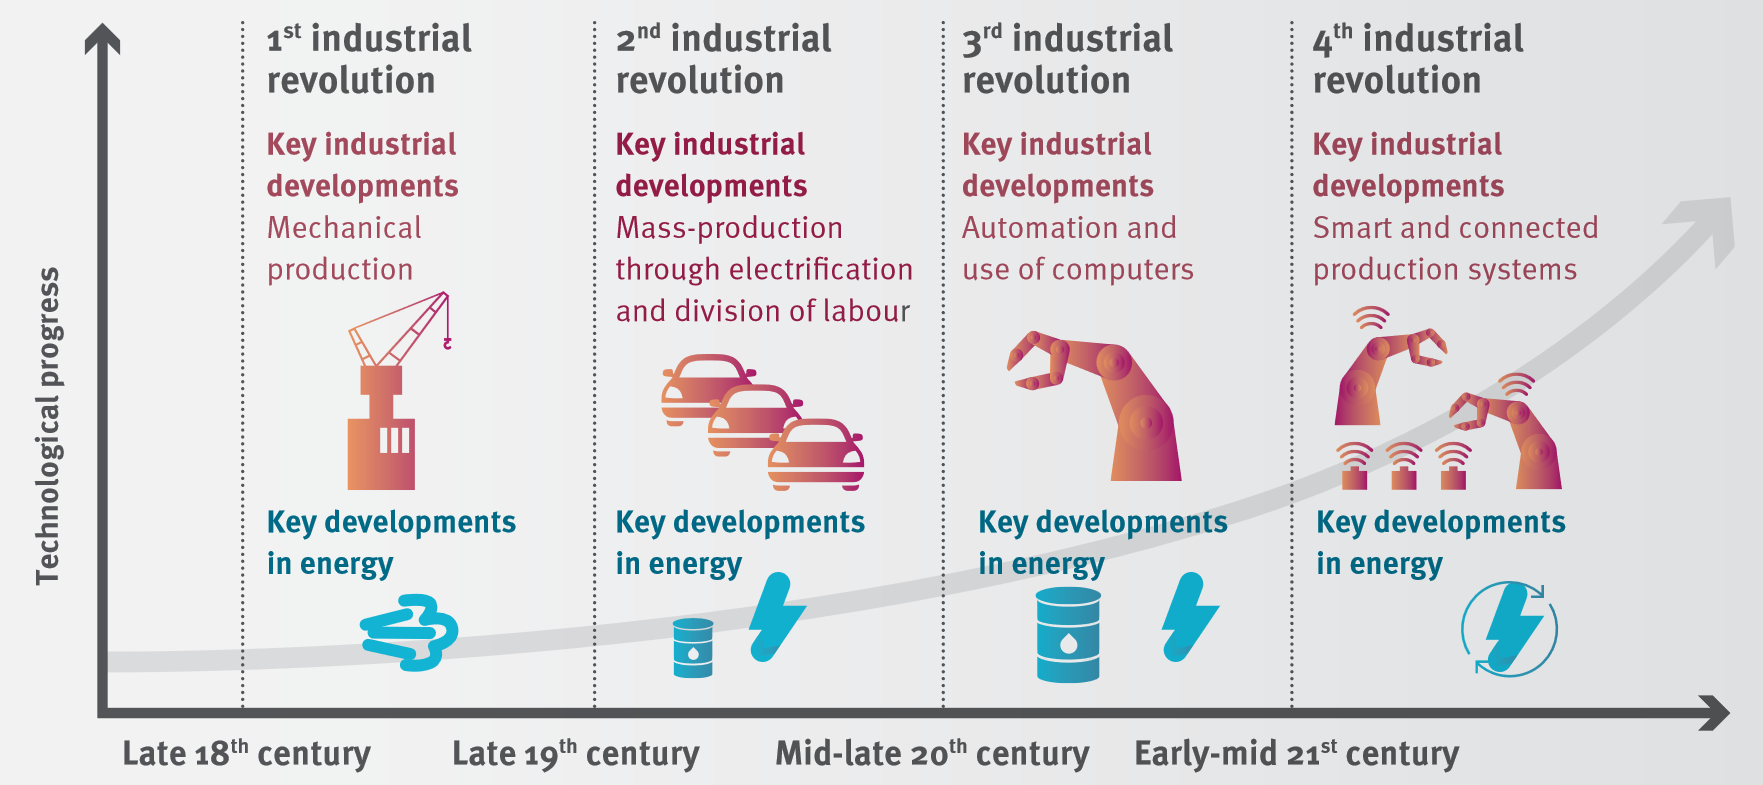
\includegraphics[scale=0.33]{industry4}
    }
    \caption{Industrial revolutions and key developments in energy change \cite{UNIDO2017}.}\label{fig:industry4}
\end{figure}

A new era of technological and social transformation is reshaping consumer expectations for energy systems, with the following required features \autocite{kholkin2025energy}:
\begin{itemize}
    \item  \textbf{Quality}: capability of power supply systems to meet the growing digital demand segment by delivering electricity with high reliability and performance standards, supported by energy storage systems (ESS), power electronics and digital control technologies.
    
    \item  \textbf{Autonomy}: energy resilience of settlements, individual consumers, mobile devices, and transport systems, enabled by local generation, storage, high-density energy conversion and smart grids, reducing reliance on centralized power and fuel supply.
    
    \item  \textbf{Intelligence}: digital modeling, scalable architectures, and digital markets enable dynamic energy exchange, automated control of complex infrastructure, and customized services to meet evolving demand.
\end{itemize}

\nomenclature{\(ESS\)}{Energy Storage Systems}


% \section{Challenges in microgrid operation and control}
\textbf{Challenges in microgrid operation and control.}
To satisfy consumer expectations, the global energy landscape is undergoing a significant transformation, driven by the increasing adoption of distributed energy systems that integrate various energy sources, including renewable generation (solar, wind), ESS, electric vehicles (EV) and controllable loads. Furthermore, the integration of renewable energy resources (RES) and distributed energy resources (DER) into the grid is typically achieved through inverter-based resources (IBR). The significant benefits of such systems in terms of energy security, sustainability, and economic efficiency, lead power grids to evolve into power electronics dominated grids (PEDG) \autocite{mag_ipakchi_2009}, as shown in Figure~\cref{fig:bulk2pedg}. This transition results in an amplified complexity and significance for device and system-level control schemes to maintain resiliency, reliability and operational stability \autocite{mag_khan_2020}. 

\nomenclature{\(EV\)}{Electric Vehicles}
\nomenclature{\(PEDG\)}{Power Electronics Dominated Grid}
\nomenclature{\(DER\)}{Distributed Energy Resources}
\nomenclature{\(IBR\)}{Inverter-Based Resources}
\nomenclature{\(RES\)}{Renewable Energy Resources}

\begin{figure}[ht]
    \centerfloat{
        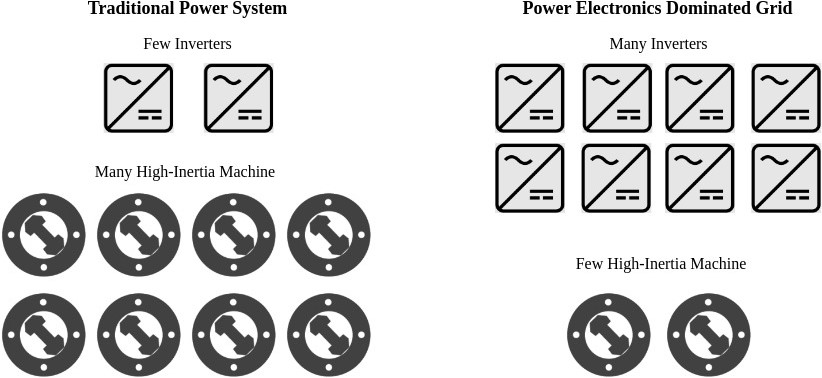
\includegraphics[scale=0.7]{bulk2pedg}
    }
    \caption{Transformation of energy paradigm.}\label{fig:bulk2pedg}
\end{figure}

As can be seen in Figure~\cref{fig:pedg_time}, the characteristic time scale of power electronics devices ranges from microseconds to milliseconds, introducing rapid control loops for voltage, current and phase-locked loops (PLL) of the network inverters. In other words, PEDG has low mechanical inertia and rapid and multi-timescale dynamics \autocite{7182342}, while also considering the inherent stochastic nature of its energy resources.

\nomenclature{\(PLL\)}{Phase-Locked Loop}

The reduced presence of synchronous machines in PEDG compared to static power electronics-based generators has a substantial impact on system inertia. PEDG exhibit significantly lower inertia than bulk interconnected power systems. This low inertia, coupled with the low short-circuit capacity of the network, exacerbates the challenge of maintaining stability. Even minor deviations in PEDG architecture due to intentional load or generator disconnections can lead to drastic fluctuations in voltage and frequency. The mixture of synchronous machines and inverter-based generation units introduces a combination of large and small time constants in PEDG, potentially causing unintended shutdowns of inverter-based generation units during system perturbations.

\begin{figure}[ht]
    \centerfloat{
        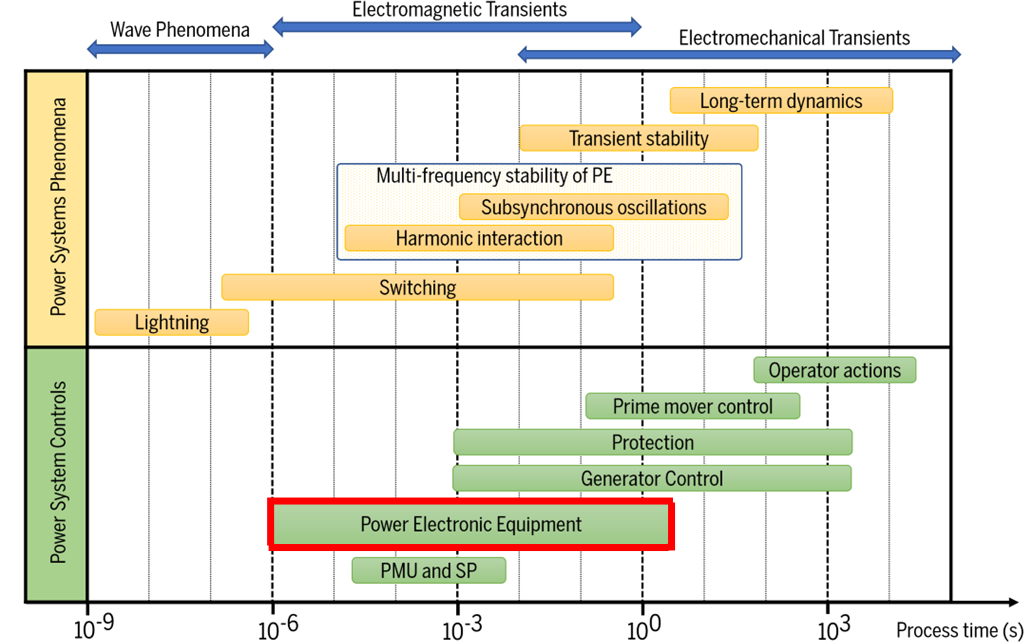
\includegraphics[scale=0.55]{pedg_time}
    }
    \caption{Characteristic operational time of PEDG \autocite{misc_karawita_2024}.}\label{fig:pedg_time}
\end{figure}

The intermittent nature of renewable energy sources in PEDG poses significant challenges for balancing demand and supply \autocite{7790991,7442160}. Moreover, the bidirectional power flow inherent in PEDG necessitates complex control and protection coordination among prosumers. It affects short-circuit current calculations and protection system design \autocite{4112346}, where engineers must consider the reserve for increased fault current magnitudes and the need to adjust protection settings to account for changed system characteristics. 

Furthermore, compared to the traditional bulk power system, PEDG exhibits unique characteristics due to the proximity of generation and load, resulting in shorter feeders and a lower inductance-resistance ratio (X/R) of grid impedance. In turn, it makes voltage control more challenging, requiring a careful management of reactive power \autocite{7749289}. 

Another key aspect, related with X/R ratio, is the equivalent impedance of the grid. The grid impedance plays a crucial role in determining the performance of IBRs. The performance of inverters is influenced not only by the inherent impedance of the power lines but also by the equivalent grid impedance at the Point of Common Coupling (PCC) as determined by the Thevenin equivalent circuit in Figure~\cref{fig:thevenin}. This impedance can be altered by the connection of parallel-connected inverters, further impacting the operation of other grid-connected devices \autocite{Jayasinghe2021}.

\nomenclature{\(PCC\)}{Point of Common Coupling}

\begin{figure}[ht]
    \centerfloat{
        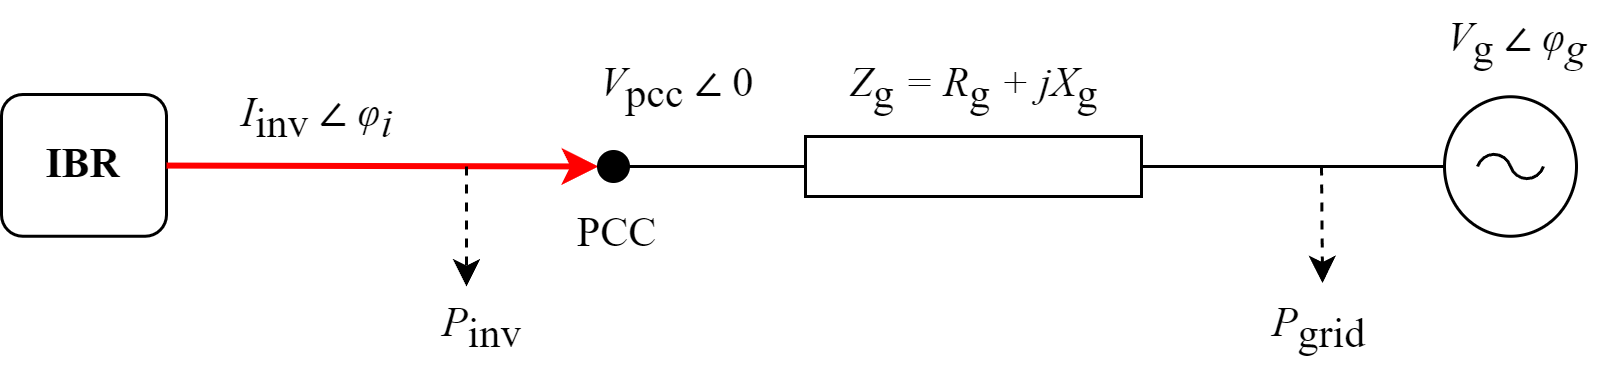
\includegraphics[scale=1.1]{thevenin}
    }
    \caption{Thevenin equivalent circuit of the grid-connected generation system.}\label{fig:thevenin}
\end{figure}

As the interconnection between multi-parallel inverters is established through the grid impedance, as shown in Figure~\cref{fig:multi_parallel}, the connection or disconnection of an inverter induces changes in the impedance seen by other inverters. This can threaten the ability of the power system to return to its normal conditions after disturbance, which is the stability of these inverters \autocite{10615092}, what is particularly relevant for low-voltage distribution systems with a lot of DERs. The fast dynamics of IBRs along with the inverter system moving to stable or unstable region can be resulted in current oscillations, as shown in Figure~\cref{fig:stability_regions}.

\begin{figure}[ht]
    \centerfloat{
        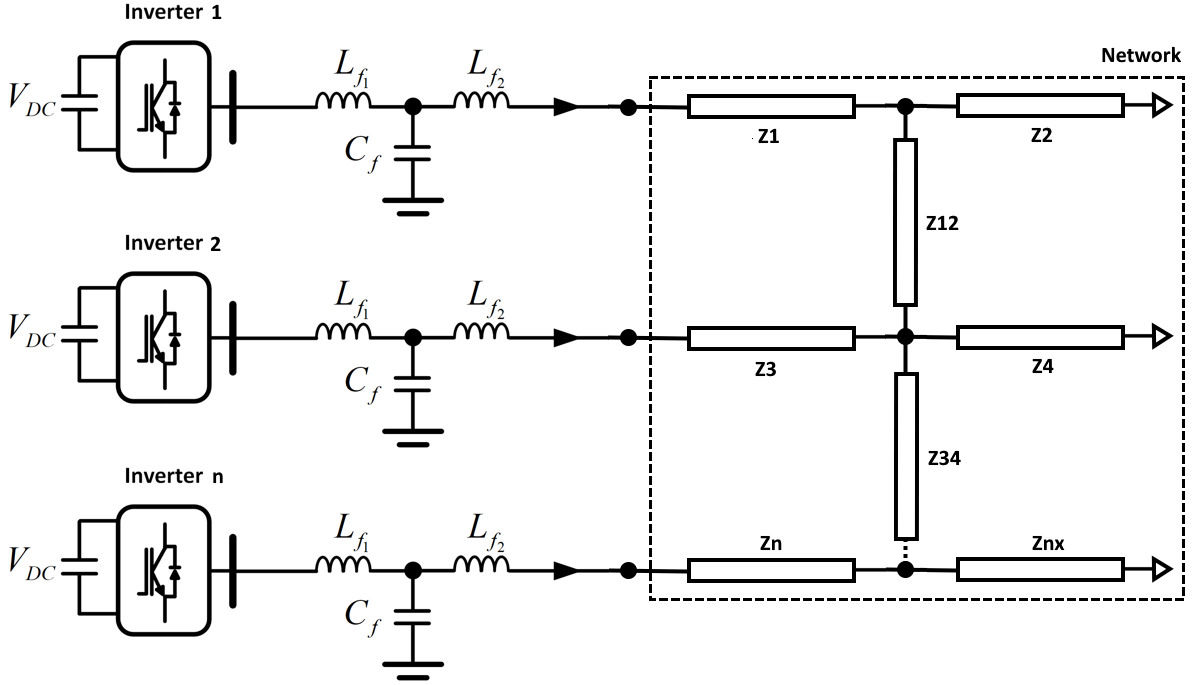
\includegraphics[scale=2]{multi_parallel}
    }
    \caption{Typical configuration of multiple paralleled inverters within a microgrid.}\label{fig:multi_parallel}
\end{figure}

\begin{figure}[ht]
    \centerfloat{
        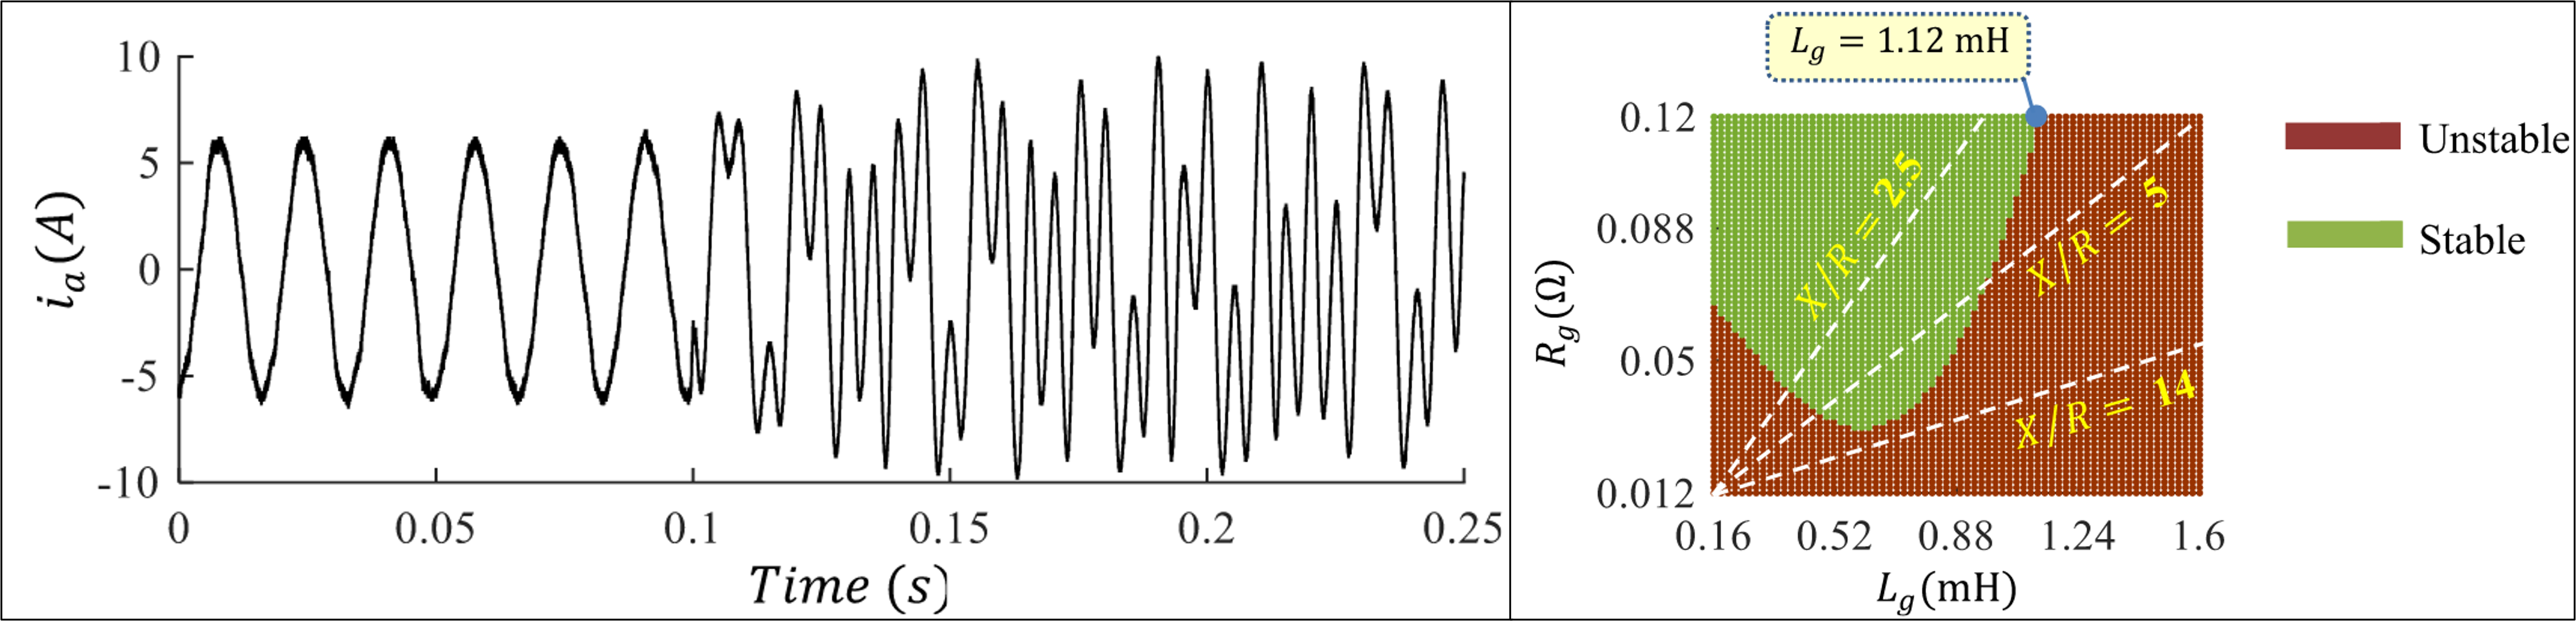
\includegraphics[scale=0.5]{stability_reg}
    }
    \caption{The stable and unstable regions with respect to X/R ratio \cite{8242351}.}\label{fig:stability_regions}
\end{figure}

The transition to PEDGs, driven by the integration of distributed generation, EVs and storage systems, introduces significant operational challenges evolving from low inertia, rapid dynamics, bidirectional power flow and stochastic behavior. The European project MIGRATE has outlined in \autocite{MIGRATE2016} the primary technical challenges associated with the extensive integration of IBRs into the grid. These challenges are summarized in Table \ref{tab:power_system_issues}, which was generalized for different level of systems and presented in Figure~\cref{fig:general_issues}  in \autocite{8809097}.

\begin{table} [htbp]
    \centering
    \begin{threeparttable}% выравнивание подписи по границам таблицы
        \caption{Ranked Issues in Power Systems}\label{tab:power_system_issues}%
        \begin{tabular}{| c || p{13cm} |}
            \hline
            \hline
                \textbf{Rank} & \textbf{Issue} \\ \hline
                1 & Decrease of inertia \\ \hline
                2 & Resonances due to cables and IBR \\ \hline
                3 & Reduction of transient stability margins \\ \hline
                4 & Missing or wrong participation of IBR-connected generators and loads in frequency containment \\ \hline
                5 & IBR Controller interaction with each other and passive AC components \\ \hline
                6 & Loss of devices in the context of fault-ride-through capability \\ \hline
                7 & Lack of reactive power \\ \hline
                8 & Introduction of new power oscillations and/or reduced damping of existing power oscillations \\ \hline
                9 & Excess of reactive power \\ \hline
                10 & Voltage dip-induced frequency dip \\ \hline
                11 & Altered static and dynamic voltage dependence of loads \\ \hline
            \hline
        \end{tabular}
    \end{threeparttable}
\end{table}

\begin{figure}[ht]
    \centerfloat{
        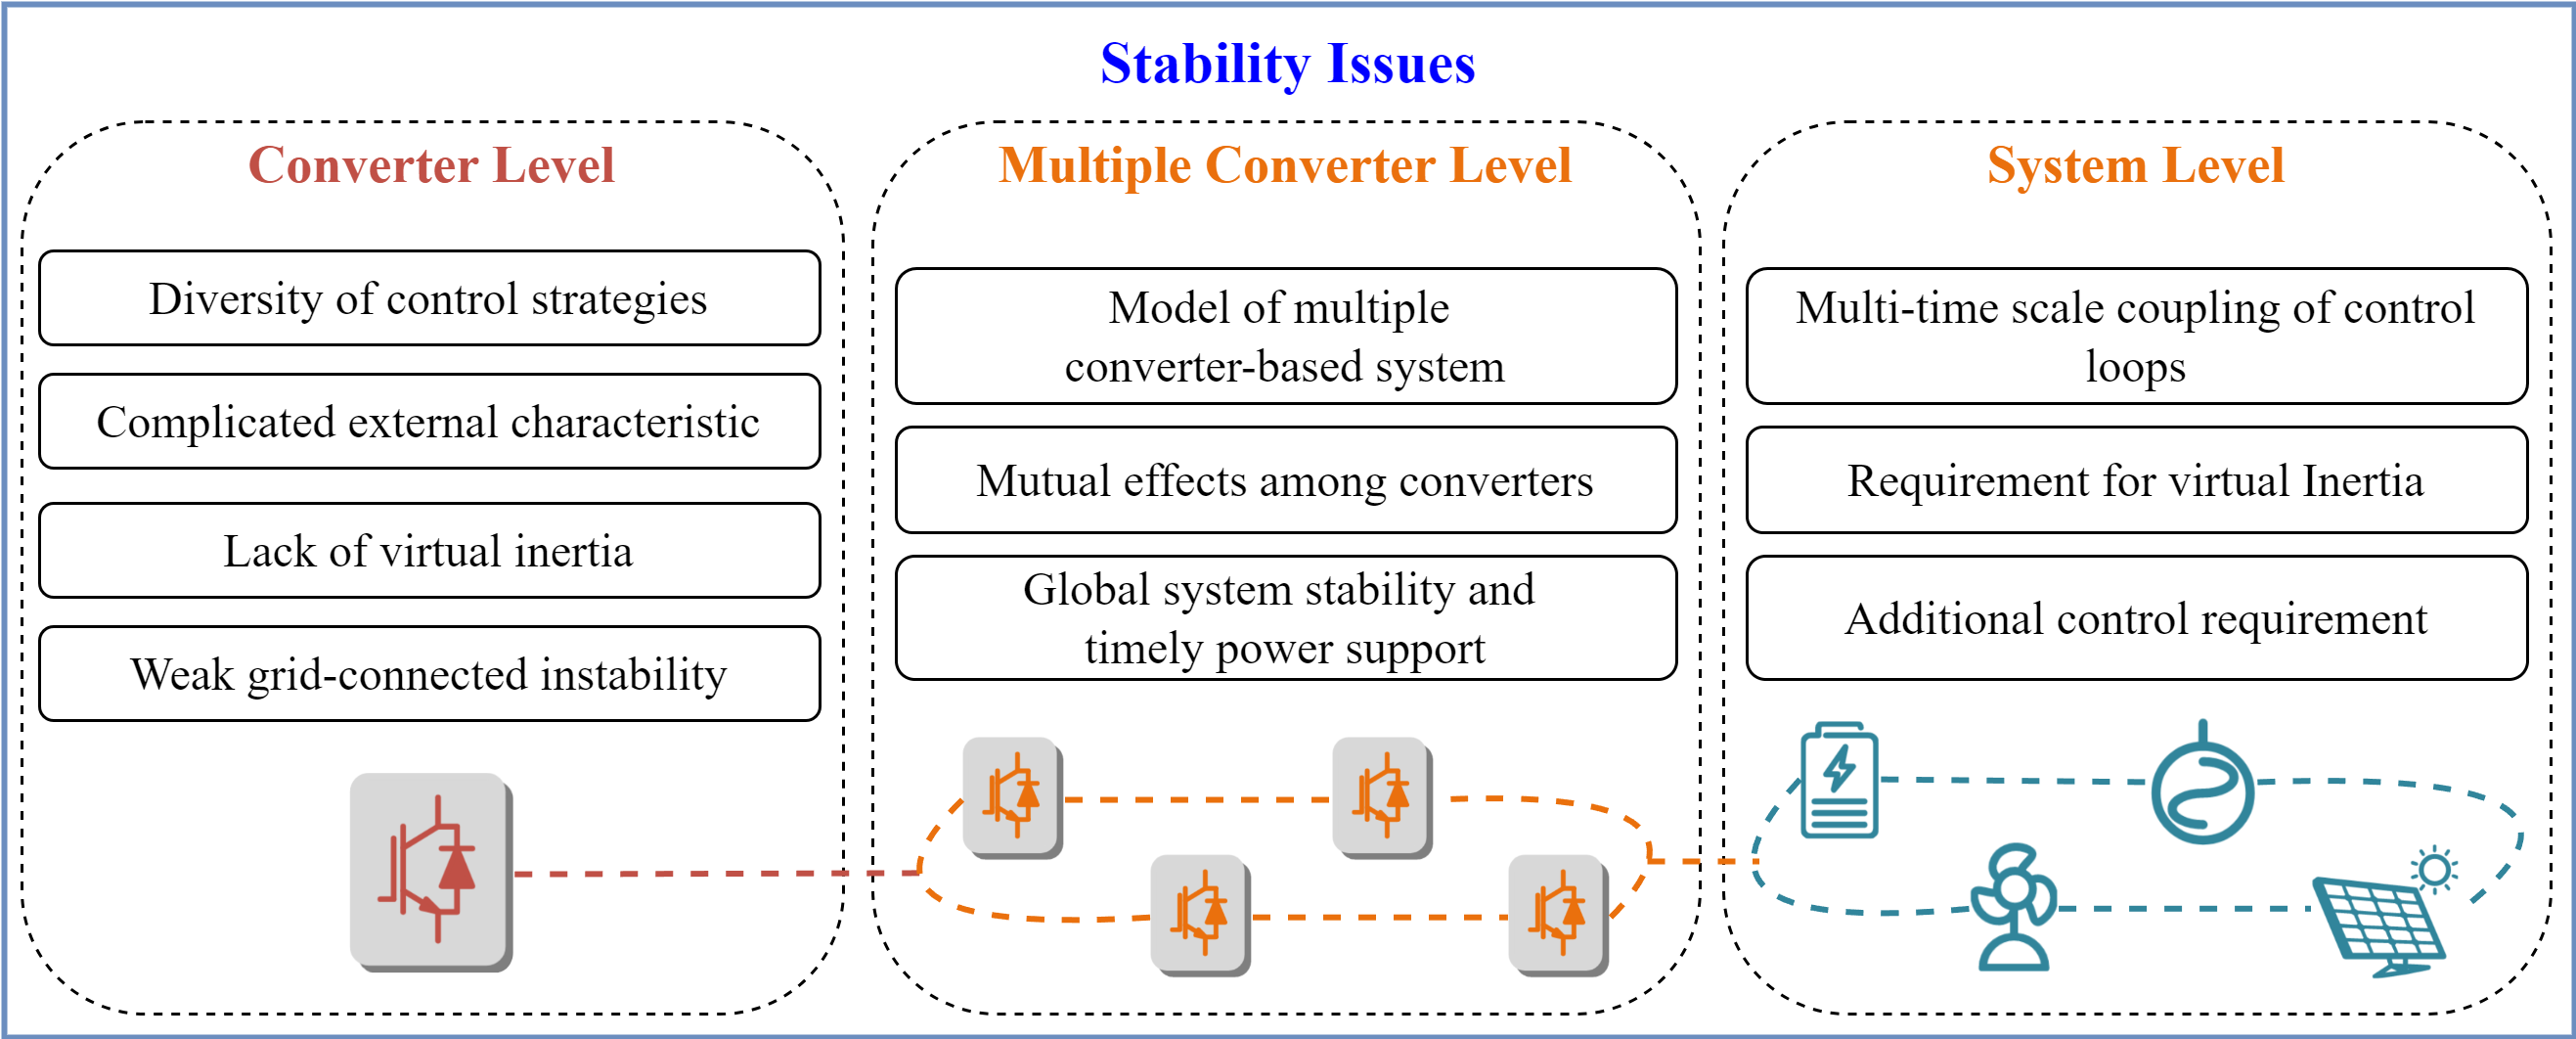
\includegraphics[scale=0.7]{general_issues}
    }
    \caption{General issues of PEDGs.}\label{fig:general_issues}
\end{figure}

Such characteristics require a paradigm shift in grid management, demanding real-time system awareness beyond the capabilities of traditional monitoring methods. The diverse timescales of PEDG dynamics, from microsecond-level converter control to minute-level demand-supply balancing, require fast and accurate dynamic state tracking to enable rapid instability detection, dynamic control and protection coordination, adaptive protection schemes, and optimized reactive power management. Maintaining secure operation of the system is one of the priority tasks, which critically depends on the system's overall observability.


\textbf{Moving Towards a DT-centric EMS Architecture.}
The electrical power system contains a transmission system, sub-transmission system, and distribution systems \autocite{kundur1994power}. As can be seen from Figure~\cref{fig:ps_illustration}, there is a comprehensive electrical interconnection among all components of the power system, whereas different voltage levels are interfaced by transformers. The fundamental role of a power system is to deliver electrical energy that meets predefined standards of quality, adequacy, reliability, and economic efficiency. 

\begin{figure}[ht]
    \centerfloat{
        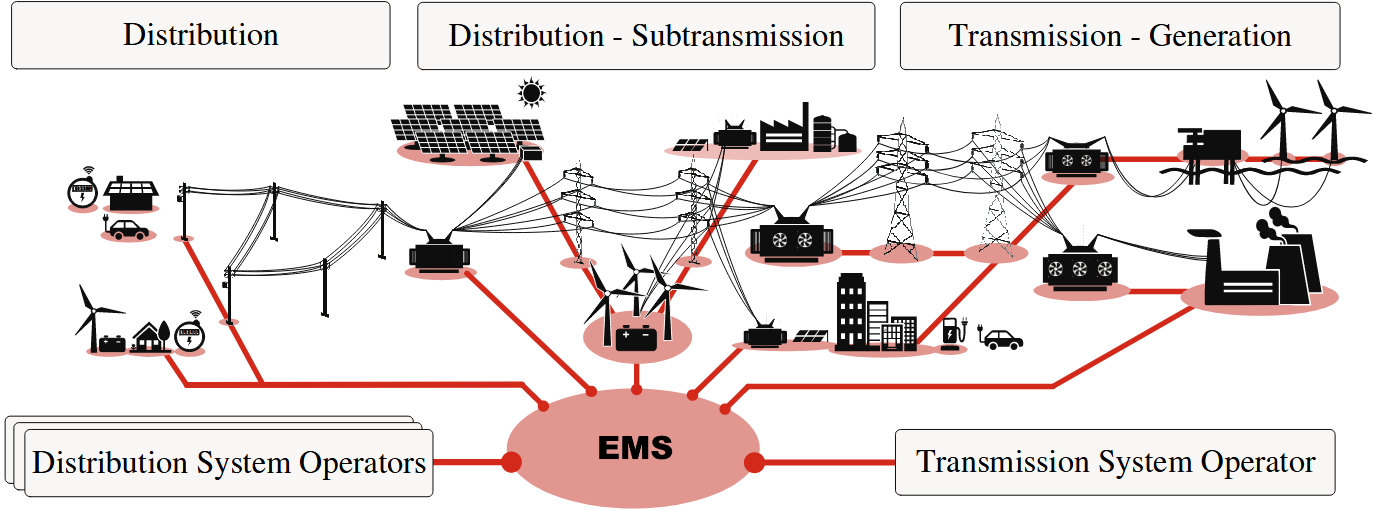
\includegraphics[scale=0.4]{ps_illustration_ems}
    }
    \caption{Illustration of modern power system \cite{Prostejovsky2017}.}\label{fig:ps_illustration}
\end{figure}

However, beyond these physical connections, maintaining secure operation critically depends on the system's overall observability. This real-time awareness of the operational state is accomplished through the deployment of numerous sensors, robust data processing infrastructure, and sophisticated information and communication technologies (ICT). The integration of the physical power infrastructure with this digital layer of monitoring and control establishes the modern power grid as a cyber-physical system. 

\nomenclature{\(ICT\)}{Information and Communication Technologies}

As the central "nerve system" of a cyber-physical entity, the Energy Management System (EMS) is designed to monitor, control, and optimize the generation, transmission, and distribution of electrical power. The aforementioned challenges in microgrid operation and control increase the complexity to EMS functioning as well. Among these intricacy's: 

\nomenclature{\(EMS\)}{Energy Management System}

\begin{itemize}
    \item Rapid change in power system operation challenges human operators in their supervision and control duties \autocite{cigre_700}.
    
    \item Complex dynamic phenomena of PEDG reduce reaction time and the capability of humans to react appropriately. This raises the risk of human errors subjected to time pressure \autocite{HAASS20155285}.
    
    \item Online dynamic security assessments (DSA) were traditionally used during planning and system design. Currently, annual dynamic stability assessments are required to determine stability limits \autocite{european_union_2017_1485}. The focus on dynamic system models has since advanced towards real-time operations.

    \item  Operating the system closer to its physical boundaries \autocite{8295027}, as necessitated by the energy transition, means that understanding and predicting these fast dynamic phenomena becomes crucial for maintaining operational security in EMS.
    
\end{itemize}

\nomenclature{\(DSA\)}{Dynamic Security Assessment}

Thus, as a response to EMS needs to address possible future scenarios and utility needs, the concept of the Digital Twin (DT) appears. Generally, DTs are digital replicas of systems, processes, or objects that mirror their physical state through abstraction and connect the physical and digital realms through sensor data streams \autocite{10311709}. The concept showed potential for applications that need improved observability and prediction of future conditions and system states. \autocite{eyre_untangling_2020}. Among the main characteristics, DT incorporates:
\begin{enumerate}
    \item A robust analytical model derived from the digital replica of the actual system \autocite{Trauer_2020},
    \item Real-time bidirectional data interaction \autocite{VANDERHORN2021113524},
    \item Accurate state reflection of the linked physical entity \autocite{JONES202036}.
\end{enumerate}

\nomenclature{\(DT\)}{Digital Twin}

Simply saying, a Digital Twin can be described dynamically updating model providing analytical insights into its mirrored system , distinguishing itself from traditional simulation models by ability to stay synchronous to the connected system. Table \ref{tab:ems_evol} illustrates the evolution of the power system evolving into a highly integrated cyber-physical system, with the DT concept as a key component of the EMS.

\begin{table} [htbp]
    \centering
    \begin{threeparttable}% выравнивание подписи по границам таблицы
        \caption{Evolution of EMS \autocite{8398846}}\label{tab:ems_evol}%
        \begin{tabular}{| c || p{5cm} | p{8cm} |}
            \hline
            \hline
                 \textbf{Generation} & \textbf{EMS Features} & \textbf{Functionality}\\ \hline
                1st & Analog communication via hardwired connections & Essential measurement values are displayed using a basic human-machine interface \\ \hline
                2nd & IP/TCP based  communication & SCADA and state estimation allow quasi steady-state observability \\ \hline
                3rd & Support of dynamic  observability & Wide area monitoring and dynamic security assessment tool available \\ \hline
                4th & Digital Twin centric architecture & Real-time simulation of high-fidelity models is a core functionality \\ \hline
            \hline
        \end{tabular}
    \end{threeparttable}
\end{table}

From the third generation of EMS, with its dynamic power system observability, the next advance is expected to be towards a DT-centric EMS architecture \autocite{dbt_mods_00054812}. In the core of that system, a modeling engine, a so-called \textit{dynamic digital mirror} (DDM), which supports real-time dynamic power system simulations. The primary focus of this research is on developing \textit{dynamic mirroring} specifically tailored for PEDGs.

\nomenclature{\(DDM\)}{Dynamic Digital Mirror}

The time-domain simulation engine, linked to the validated DT simulation model, allows precise state representation of the observed power system. This dynamic digital mirror engine aids in accurately estimating the power system state and provides a validated model foundation, potentially facilitating online power system studies like dynamic security analysis, state health monitoring, forecasting, event identification, relay protection and cyber security. The proposed method is evaluated through case studies using real-time numerical time-domain simulations, aiming for accurate and reliable dynamic mirroring.

{\aim} of the study is to develop a method for dynamic mirroring in PEDGs using a digital twin approach. 

To achieve the goal of the dissertation, the following {\tasks} are addressed:
\begin{enumerate}[beginpenalty=10000] % https://tex.stackexchange.com/a/476052/104425
  \item To propose an architecture of digital dynamic mirroring for the next generation of monitoring system.
  \item To develop an accurate and computationally effective modeling approach for a power system DT.
  \item To develop DT simulation engine to run real-time dynamic PEDG simulations.
  \item To develop of corresponding communication interfaces to apply the dynamic mirroring for online system monitoring.
\end{enumerate}


{\novelty} which are also {\defpositions}
\begin{enumerate}[beginpenalty=10000] % https://tex.stackexchange.com/a/476052/104425
  \item Validated dynamic average models for key components suitable for representation of dynamics of PEDG in real-time simulation.
  \item A novel DT framework for dynamic mirroring in PEDGs.
  \item Analysis of the sensitivity of the DT-based DDM to parameter deviations and data latency.
\end{enumerate}

{\influence} of the research. The main conclusions of the dissertation research can be used for developing the core component of next-generation DT-centric EMS, a suitable modeling engine, which allows for mirroring the actual power system state to support control, decision-making, and to execute simulations to predict future states. 

% The thesis presents the novel approach for DDM as a part of the next generation EMS. The effective modeling approach and simulation engine for real-time DT model execution developed by author.

{\methods} The methodology is based on applying discrete time state-space modeling for real-time simulation engine to run the dynamic model of PEDG. The research is based on comprehensive analysis of fast dynamics which appear in PEDG and arise from the interaction of numerous IBRs and transmission lines. The research include inverter grid-following mode dynamic modeling on behalf of TL and loads.  The research was validated through numerical real-time simulations and laboratory experiments based on hardware-in-the-loop approach. 

% {\defpositions}
% \begin{enumerate}[beginpenalty=10000] % https://tex.stackexchange.com/a/476052/104425
%   \item Первое положение
%   \item Второе положение
%   \item Третье положение
%   \item Четвертое положение
% \end{enumerate}
% В папке Documents можно ознакомиться с решением совета из Томского~ГУ
% (в~файле \verb+Def_positions.pdf+), где обоснованно даются рекомендации
% по~формулировкам защищаемых положений.


{\reliability} were confirmed by numerical simulation and experimental validation with hardware-in-loop approach involved de facto RTDS and OPAL-RT tools for the closed-loop testing of electrical hardware systems. The statements and conclusions formulated in the dissertation have been approved by the committees of experts in international scientific conferences. The credibility is also confirmed by the publications of research results in peer-reviewed scientific journals. 


{\probation}
The results of the dissertation were presented at the following international conferences:
\begin{itemize}
    \item 25th International Conference of Young Professionals in Electron Devices and Materials (2024 EDM).
    \item Conference of Young Researchers in Electrical and Electronic Engineering (2025 ElCon)
\end{itemize}

{\contribution} The personal contribution of the author includes proposing the idea of dynamic mirroring based on DT approach. To prove it, the author develop computationally efficient dynamic average models of PEDG for real-time execution, aiming to provide accurate and timely grid observability, even during transient events. For testing, hardware-in-the-loop test bench was developed, including physical grid representation and a DT model with data measurement interaction between them. All real-time simulations were performed and finally validated through experiments. 

% \ifnumequal{\value{bibliosel}}{0}
% {%%% Встроенная реализация с загрузкой файла через движок bibtex8. (При желании, внутри можно использовать обычные ссылки, наподобие `\cite{vakbib1,vakbib2}`).
%     {\publications} Основные результаты по теме диссертации изложены
%     в~XX~печатных изданиях,
%     X из которых изданы в журналах, рекомендованных ВАК,
%     X "--- в тезисах докладов.
% }%
% {%%% Реализация пакетом biblatex через движок biber
%     \begin{refsection}[bl-author, bl-registered]
%         % Это refsection=1.
%         % Процитированные здесь работы:
%         %  * подсчитываются, для автоматического составления фразы "Основные результаты ..."
%         %  * попадают в авторскую библиографию, при usefootcite==0 и стиле `\insertbiblioauthor` или `\insertbiblioauthorgrouped`
%         %  * нумеруются там в зависимости от порядка команд `\printbibliography` в этом разделе.
%         %  * при использовании `\insertbiblioauthorgrouped`, порядок команд `\printbibliography` в нём должен быть тем же (см. biblio/biblatex.tex)
%         %
%         % Невидимый библиографический список для подсчёта количества публикаций:
%         \phantom{\printbibliography[heading=nobibheading, section=1, env=countauthorvak,          keyword=biblioauthorvak]%
%         \printbibliography[heading=nobibheading, section=1, env=countauthorwos,          keyword=biblioauthorwos]%
%         \printbibliography[heading=nobibheading, section=1, env=countauthorscopus,       keyword=biblioauthorscopus]%
%         \printbibliography[heading=nobibheading, section=1, env=countauthorconf,         keyword=biblioauthorconf]%
%         \printbibliography[heading=nobibheading, section=1, env=countauthorother,        keyword=biblioauthorother]%
%         \printbibliography[heading=nobibheading, section=1, env=countregistered,         keyword=biblioregistered]%
%         \printbibliography[heading=nobibheading, section=1, env=countauthorpatent,       keyword=biblioauthorpatent]%
%         \printbibliography[heading=nobibheading, section=1, env=countauthorprogram,      keyword=biblioauthorprogram]%
%         \printbibliography[heading=nobibheading, section=1, env=countauthor,             keyword=biblioauthor]%
%         \printbibliography[heading=nobibheading, section=1, env=countauthorvakscopuswos, filter=vakscopuswos]%
%         \printbibliography[heading=nobibheading, section=1, env=countauthorscopuswos,    filter=scopuswos]}%
%         %
%         \nocite{*}%
%         %
%         {\publications} Основные результаты по теме диссертации изложены в~\arabic{citeauthor}~печатных изданиях,
%         \arabic{citeauthorvak} из которых изданы в журналах, рекомендованных ВАК%
%         \ifnum \value{citeauthorscopuswos}>0%
%             , \arabic{citeauthorscopuswos} "--- в~периодических научных журналах, индексируемых Web of~Science и Scopus%
%         \fi%
%         \ifnum \value{citeauthorconf}>0%
%             , \arabic{citeauthorconf} "--- в~тезисах докладов.
%         \else%
%             .
%         \fi%
%         \ifnum \value{citeregistered}=1%
%             \ifnum \value{citeauthorpatent}=1%
%                 Зарегистрирован \arabic{citeauthorpatent} патент.
%             \fi%
%             \ifnum \value{citeauthorprogram}=1%
%                 Зарегистрирована \arabic{citeauthorprogram} программа для ЭВМ.
%             \fi%
%         \fi%
%         \ifnum \value{citeregistered}>1%
%             Зарегистрированы\ %
%             \ifnum \value{citeauthorpatent}>0%
%             \formbytotal{citeauthorpatent}{патент}{}{а}{}%
%             \ifnum \value{citeauthorprogram}=0 . \else \ и~\fi%
%             \fi%
%             \ifnum \value{citeauthorprogram}>0%
%             \formbytotal{citeauthorprogram}{программ}{а}{ы}{} для ЭВМ.
%             \fi%
%         \fi%
%         % К публикациям, в которых излагаются основные научные результаты диссертации на соискание учёной
%         % степени, в рецензируемых изданиях приравниваются патенты на изобретения, патенты (свидетельства) на
%         % полезную модель, патенты на промышленный образец, патенты на селекционные достижения, свидетельства
%         % на программу для электронных вычислительных машин, базу данных, топологию интегральных микросхем,
%         % зарегистрированные в установленном порядке.(в ред. Постановления Правительства РФ от 21.04.2016 N 335)
%     \end{refsection}%
%     \begin{refsection}[bl-author, bl-registered]
%         % Это refsection=2.
%         % Процитированные здесь работы:
%         %  * попадают в авторскую библиографию, при usefootcite==0 и стиле `\insertbiblioauthorimportant`.
%         %  * ни на что не влияют в противном случае
%         \nocite{vakbib2}%vak
%         \nocite{patbib1}%patent
%         \nocite{progbib1}%program
%         \nocite{bib1}%other
%         \nocite{confbib1}%conf
%     \end{refsection}%
%         %
%         % Всё, что вне этих двух refsection, это refsection=0,
%         %  * для диссертации - это нормальные ссылки, попадающие в обычную библиографию
%         %  * для автореферата:
%         %     * при usefootcite==0, ссылка корректно сработает только для источника из `external.bib`. Для своих работ --- напечатает "[0]" (и даже Warning не вылезет).
%         %     * при usefootcite==1, ссылка сработает нормально. В авторской библиографии будут только процитированные в refsection=0 работы.
% }

% При использовании пакета \verb!biblatex! будут подсчитаны все работы, добавленные
% в файл \verb!biblio/author.bib!. Для правильного подсчёта работ в~различных
% системах цитирования требуется использовать поля:
% \begin{itemize}
%         \item \texttt{authorvak} если публикация индексирована ВАК,
%         \item \texttt{authorscopus} если публикация индексирована Scopus,
%         \item \texttt{authorwos} если публикация индексирована Web of Science,
%         \item \texttt{authorconf} для докладов конференций,
%         \item \texttt{authorpatent} для патентов,
%         \item \texttt{authorprogram} для зарегистрированных программ для ЭВМ,
%         \item \texttt{authorother} для других публикаций.
% \end{itemize}
% Для подсчёта используются счётчики:
% \begin{itemize}
%         \item \texttt{citeauthorvak} для работ, индексируемых ВАК,
%         \item \texttt{citeauthorscopus} для работ, индексируемых Scopus,
%         \item \texttt{citeauthorwos} для работ, индексируемых Web of Science,
%         \item \texttt{citeauthorvakscopuswos} для работ, индексируемых одной из трёх баз,
%         \item \texttt{citeauthorscopuswos} для работ, индексируемых Scopus или Web of~Science,
%         \item \texttt{citeauthorconf} для докладов на конференциях,
%         \item \texttt{citeauthorother} для остальных работ,
%         \item \texttt{citeauthorpatent} для патентов,
%         \item \texttt{citeauthorprogram} для зарегистрированных программ для ЭВМ,
%         \item \texttt{citeauthor} для суммарного количества работ.
% \end{itemize}
% % Счётчик \texttt{citeexternal} используется для подсчёта процитированных публикаций;
% % \texttt{citeregistered} "--- для подсчёта суммарного количества патентов и программ для ЭВМ.

% Для добавления в список публикаций автора работ, которые не были процитированы в
% автореферате, требуется их~перечислить с использованием команды \verb!\nocite! в
% \verb!Synopsis/content.tex!.
 % Характеристика работы по структуре во введении и в автореферате не отличается (ГОСТ Р 7.0.11, пункты 5.3.1 и 9.2.1), потому её загружаем из одного и того же внешнего файла, предварительно задав форму выделения некоторым параметрам

\textbf{Approbation of the work.} The dissertation consists of an introduction,
\formbytotal{totalchapter}{chapters}{}{}{}, conclusion. 
The dissertation is
\formbytotal{TotPages}{pages}{}{}{} long, including
\formbytotal{totalcount@figure}{figures}{}{}{} and
\formbytotal{totalcount@table}{tables}{}{}{}.
 The list of references contains
\formbytotal{citenum}{titles}{}{}{}.


% \formbytotal{totalchapter}{глав}{ы}{}{},
% заключения и
% \formbytotal{totalappendix}{приложен}{ия}{ий}{}.
% %% на случай ошибок оставляю исходный кусок на месте, закомментированным
% %Полный объём диссертации составляет  \ref*{TotPages}~страницу
% %с~\totalfigures{}~рисунками и~\totaltables{}~таблицами. Список литературы
% %содержит \total{citenum}~наименований.
% %
% Полный объём диссертации составляет
% \formbytotal{TotPages}{страниц}{у}{ы}{}, включая
% \formbytotal{totalcount@figure}{рисун}{ок}{ка}{ков} и
% \formbytotal{totalcount@table}{таблиц}{у}{ы}{}.
% Список литературы содержит
% \formbytotal{citenum}{наименован}{ие}{ия}{ий}.
    % Введение
\ifnumequal{\value{contnumfig}}{1}{\counterwithout{figure}{chapter}
}{\counterwithin{figure}{chapter}}
\ifnumequal{\value{contnumtab}}{1}{\counterwithout{table}{chapter}
}{\counterwithin{table}{chapter}}
\chapter{State of the Art in Technology and Research}\label{ch:ch1}

This chapter provides a comprehensive review of available tools and methods for monitoring and control of the power system, including capturing network dynamics. As an important part of EMS, power system state estimation techniques are analyzed, where different state estimation algorithms, methodologies,  and approaches are discussed. The concept of wide area monitoring systems, which are lately deployed to capture network dynamics are explained. Among these state-of-the-art analysis, research gaps and areas that can be improved are pointed out.

\section{Energy Management System}\label{sec:ch1/sec1}

The reliable and efficient operation of modern power systems is critically dependent on sophisticated control and monitoring infrastructure. At the heart of this infrastructure stands the Energy Management System, often co-located within a power system control center. EMS acts as the central nerve system, continuously sensing the state of the grid, coordinating operational adjustments, and providing tools for system security and economic optimization \autocite{8278740}. Its functions are crucial to ensure the continuous balance between electricity generation and demand, maintaining voltage and frequency stability, managing transmission constraints, and facilitating increasingly complex market operations \autocite{Handschin_Petroianu_1991}.

Large-scale power systems are managed by a hierarchy of control centers, each responsible for specific segments of the grid based on voltage levels and system complexity. These centers include main transmission control centers, sub-transmission control centers, and distribution control centers, each with distinct roles, system visibility, and automation tailored to their operational needs. 

Power system control centers evolved from early analog systems for basic generation control and monitoring. A major driving force was the 1965 blackout \autocite{USFedEnergyComm1967}, which accelerated the adoption of digital computers, leading to the development of supervisory control and data acquisition (SCADA) systems for data collection and remote control. The introduction of system security concepts in the 1970s integrated with SCADA advanced applications like \autocite{Handschin_Petroianu_1991}: 
\begin{itemize}
    \item State Estimation (SE): Processing real-time SCADA data to provide a statistically accurate and consistent picture of the system state, crucial for downstream applications.
    \item Contingency Analysis (CA): Simulating the impact of postulated disturbances (contingencies) on the estimated system state to identify potential overloads or voltage violations.
    \item Optimal Power Flow (OPF): An optimization tool used for various purposes, including transmission-constrained economic dispatch and preventive control actions.
    \item Unit Commitment (UC): Scheduling generator startup and shutdown to meet anticipated load demand reliably at minimum cost.
\end{itemize}

\nomenclature{\(SCADA\)}{Supervisory Control and Data Acquisition}
\nomenclature{\(CA\)}{Contingency Analysis}
\nomenclature{\(UC\)}{Unit Commitment}
\nomenclature{\(SE\)}{State Estimation}
\nomenclature{\(OPF\)}{Optimal Power Flow}

From a functional perspective, a traditional EMS serves as the primary tool for power system operators, supporting real-time data acquisition, generation control, and network analysis and control.

\begin{itemize}
    \item Data Acquisition: Collect real-time measurements (voltage, current, power flows), equipment status (breaker positions, tap positions), and alarms from remote devices such as Remote Terminal Units (RTU) and Intelligent Electronic Devices (IED) in substations and power plants. These data, often collected every few seconds, provide a snapshot of the state of the system.
    \item Generation Control: Includes functions like Load Frequency Control for balancing generation and load in real-time to maintain frequency and interchange schedules, and Economic Dispatch for determining optimal generation levels to minimize cost.
    \item Network Analysis and Control: Using the data collected and a network model to assess system security and recommend control actions. This encompasses SE, CA, OPF, Security-Constrained Economic Dispatch, and increasingly, dynamic stability assessment tools.
\end{itemize}

\nomenclature{\(IED\)}{Intelligent Electronic Devices}
\nomenclature{\(RTU\)}{Intelligent Electronic Devices}

The architecture of traditional control centers evolved from centralized monolithic systems to more distributed and networked environments over time. The SCADA system typically employed a star configuration with dedicated physical communication links connecting RTUs to a central data acquisition computer \autocite{1405870}. The EMS applications ran on computers (workstations/PCs) within a Local Area Network (LAN). Inter-control center communication often relied on point-to-point networks. Figure~\cref{fig:ems_arch2} illustrates a simplified EMS architecture.

\begin{figure*}[htbp]
    \centering
    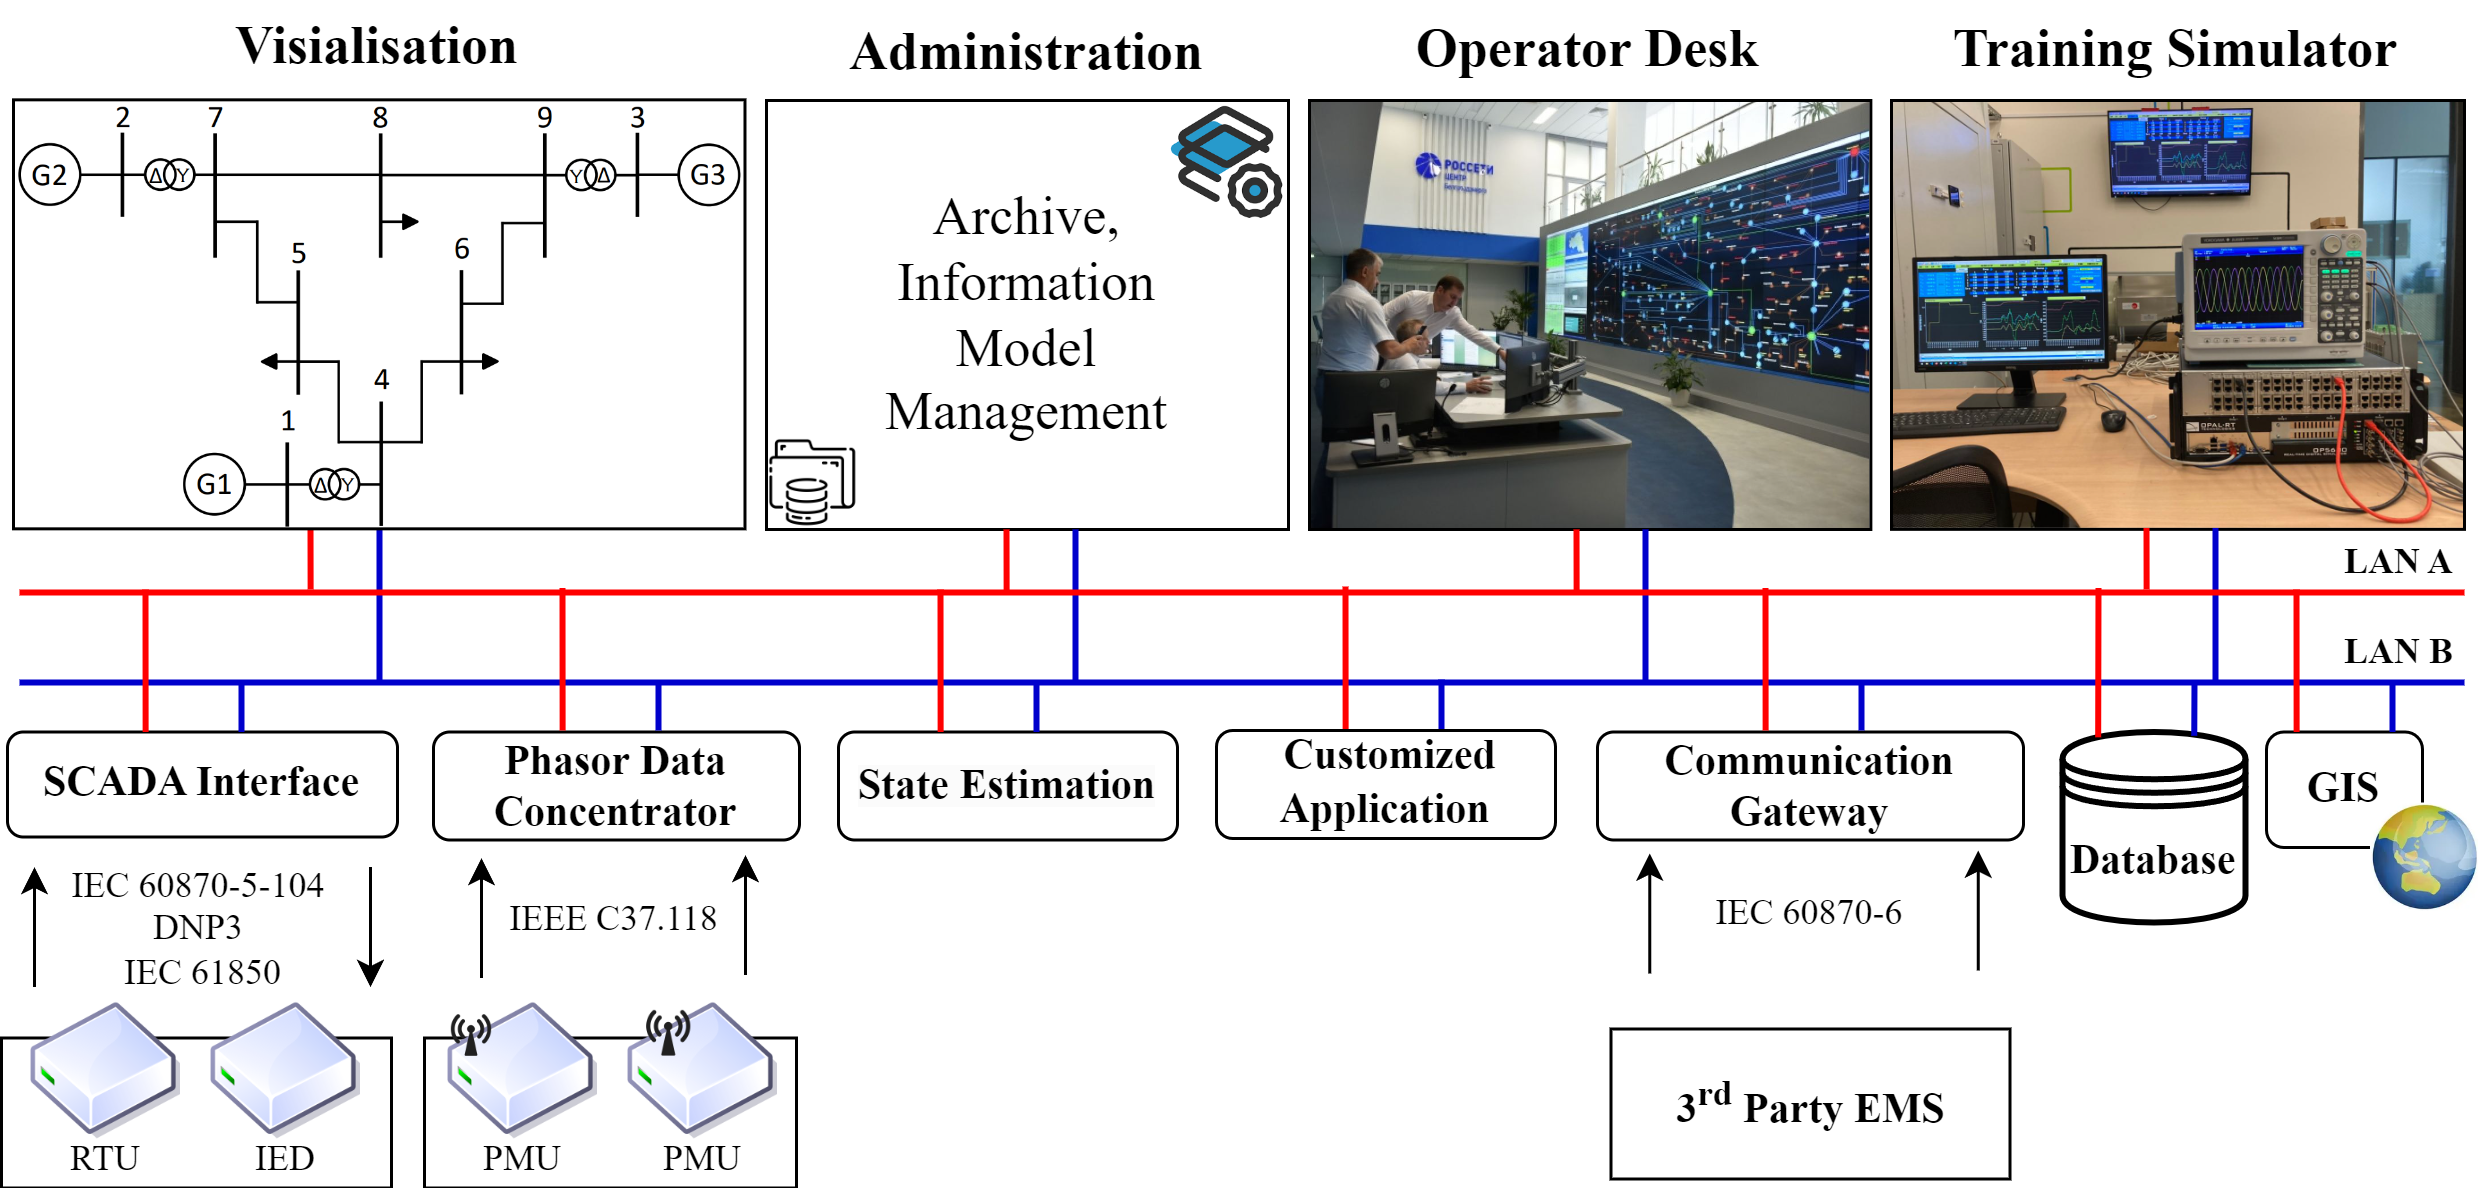
\includegraphics[width=1\textwidth]{ems_arch_2.png}
    \caption{Simplified EMS architecture.}
    \label{fig:ems_arch2}
\end{figure*}

The EMS primarily constitutes a front-end communication system responsible for data acquisition and control interactions, along with a critical Information Model Management (IMM) system. IMM contains a comprehensive topological model of the power system that details connectivity, component parameters, telemetry addresses, and telecontrol capabilities. Leveraging gathered telemetry data and the information model, the SE processes this information to yield a statistically robust and computable steady-state image of the power system's current operational state. Building upon the real-time state provided by the SE, the EMS incorporates a suite of secondary functions, also termed Advanced Decision and Optimization (ADO) functions. These applications provide essential model-based analyzes and decision support tools crucial for real-time operations and operational planning. Examples of these advanced functions include contingency screening, security assessment, switching simulations, and power flow optimization. 

\nomenclature{\(IMM\)}{Information Model Management}
\nomenclature{\(ADO\)}{Advanced Decision and Optimization }

ADO applications demand comprehensive topological information integrated with various operational degrees of freedom.  This includes predictions for load and generation, associated costs of generation, and reserves for generation. All of these factors contribute fundamentally to effectively accomplishing the intended optimization goals. Security assessment involves calculating short circuit current and protection security assessment (PSA) to evaluate protection settings, selectivity, and protection coordination of the system.

\nomenclature{\(PSA\)}{Protection Security Assessment}

Supporting these core functionalities are critical data management systems. This includes a historical data archive to store processed data, often compressed for long-term retention, and an immutable operational logbook that carefully documents all operator actions.
Access to EMS functionalities and visualized telemetry data is typically facilitated via workstation clients equipped with suitable Graphical User Interfaces (GUI). The overall control center EMS functional modules interactions visualized in Figure~\cref{fig:ems_modules_inter}.

\begin{figure*}[htbp]
    \centering
    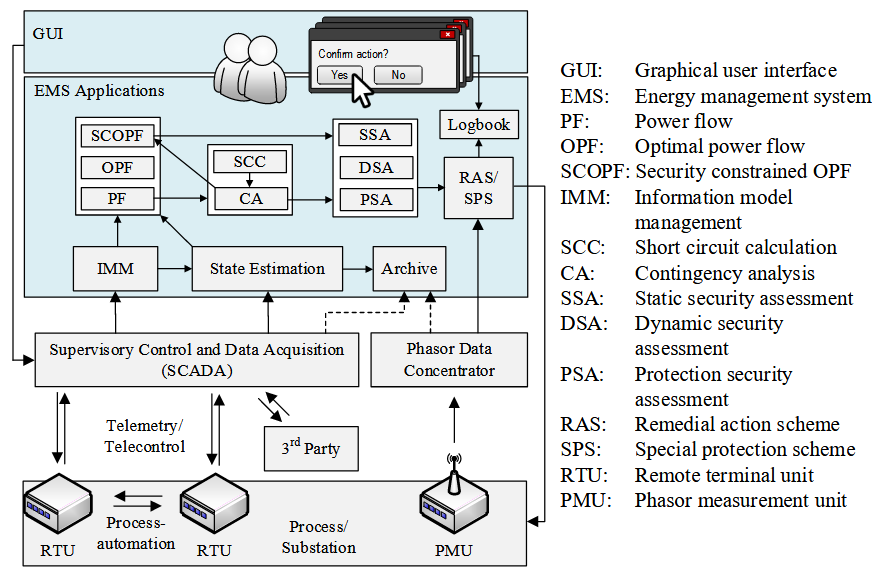
\includegraphics[width=1\textwidth]{ems_modules_interaction.png}
    \caption{Simplified EMS functional modules interaction  \autocite{8398846}.}
    \label{fig:ems_modules_inter}
\end{figure*}

Transmission systems benefit from extensive automation and real-time telemetry, while distribution systems, especially at medium- and low-voltage levels, face significant gaps in observability and controllability. This discrepancy arises from the historical design of distribution grids as passive networks, which now struggle to adapt to modern demands like renewable energy integration and real-time monitoring \autocite{8232008}.

\section{Measurement data}\label{sec:ch1/sec2}

SCADA systems and phasor measurement units (PMU) are two types of measurement systems that are commonly used for monitoring and control in power systems to ensure stability, reliability and efficiency. In general, it refers to the monitoring, control, and visualization of a technical process through computer systems that interact via an ICT network.

\nomenclature{\(PMU\)}{Phasor Measurement Units}

The integration of SCADA and PMU measurements enhances accuracy and reliability of state estimation. Although SCADA data are generally more accessible, PMU measurements offer higher accuracy and richer insights into the power system's status. SCADA measurements typically offer broad data on the power system's status, whereas PMU data provide precise insights at specific points. 

\subsection{Supervisory Control and Data Acquisition}\label{subsec:ch1/sec2/sub1}

SCADA is a combination of hardware and software used to gather real-time data from various components of the power grid. It enables operators to observe system performance, detect abnormalities, and take corrective actions either automatically or manually. SCADA typically integrates RTUs, IEDs, communication switches, merging units, programmable logic controllers (PLC), communication networks and human-machine interfaces (HMI) to maintain supervisory control over distributed assets \autocite{en12061084}. 

\nomenclature{\(PLC\)}{Programmable Logic Controller}
\nomenclature{\(HMI\)}{Human-Machine Interfaces}

The SCADA system's architecture generally comprises three key layers:
\begin{itemize}
    \item Field Layer: This level includes sensors, actuators, and devices such as RTUs, IEDs or PLCs, that collect operational data and perform local control actions.
    \item Communication Layer: Facilitates data transmission between field devices and control centers using wired or wireless networks.
    \item Control Center Layer: The central processing unit where HMIs, databases, and analytical tools are located. It is the operator's hub for system supervision and decision-making.
\end{itemize}
These layers work in coordination to provide a consistent view of the power system, allowing real-time management and historical analysis \autocite{nist_sp800_82}. In Figure~\cref{fig:scada_schematic} a SCADA system illustrated with structural components.

\begin{figure*}[htbp]
    \centering
    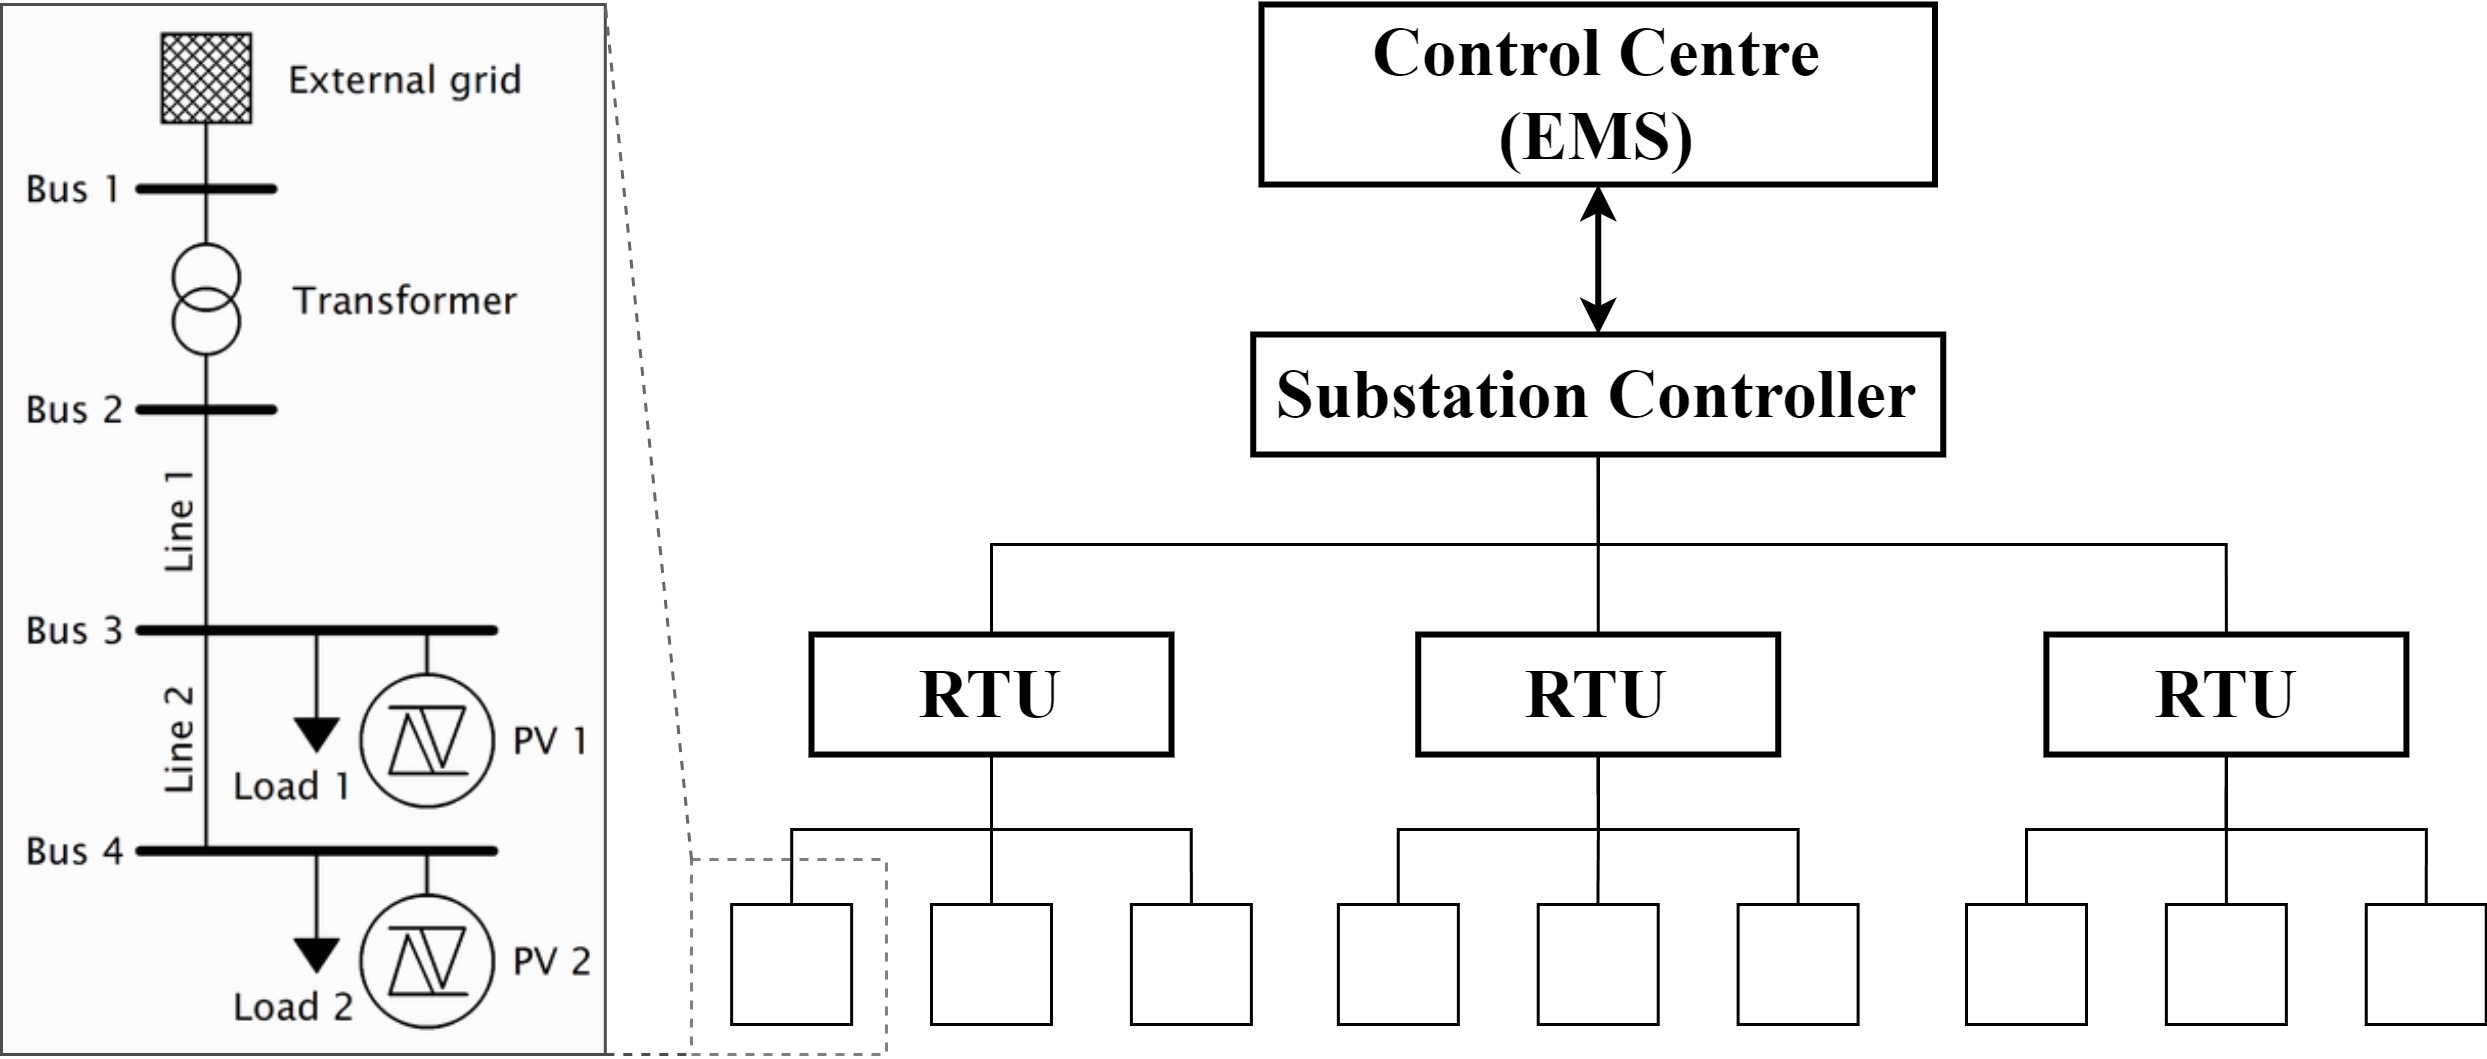
\includegraphics[width=1\textwidth]{scada_schematic2.png}
    \caption{Schematic representation of a SCADA system structure in a substation.}
    \label{fig:scada_schematic}
\end{figure*}

A modern SCADA system includes the following features:  
\begin{itemize}
    \item Real-Time Process Monitoring: Thanks to graphical visualizations and control panels, operators can immediately detect irregularities and respond quickly.
    \item Analytics and Optimization: Integrating machine learning modules and advanced analytics allow for predictive failure detection, more efficient resource management, and cost optimization.
    \item Scalability and Flexibility: Web-based SCADA solutions can be deployed in the cloud or on-premises, without limitations on the amount of process data or the number of users.
    \item Security and Easy Maintenance: Client-server architecture and use well-established encryption protocols (TLS, VPN), which greatly facilitates system protection and maintenance.
\end{itemize}

SCADA systems collect data from various sensors and devices in a power system, such as voltage and current sensors, circuit breakers and switchgear. Data transmission is realized via RTUs within substations through structured messages. 

These appear cyclically or triggered by event and contain the information itself, the cause of transmission and other relevant meta-data. The data rate depends on the device settings and the polling cycle. SCADA systems usually obtain new measurement sets every 1-10 seconds \autocite{1338122}.

Most communication occurs via fiber optic cables, whereas distribution networks frequently utilize ripple control or common telecommunication standards like LTE and GPRS for cost efficiency, as shown in Figure~\cref{fig:scada_communication}.

\begin{figure*}[htbp]
    \centering
    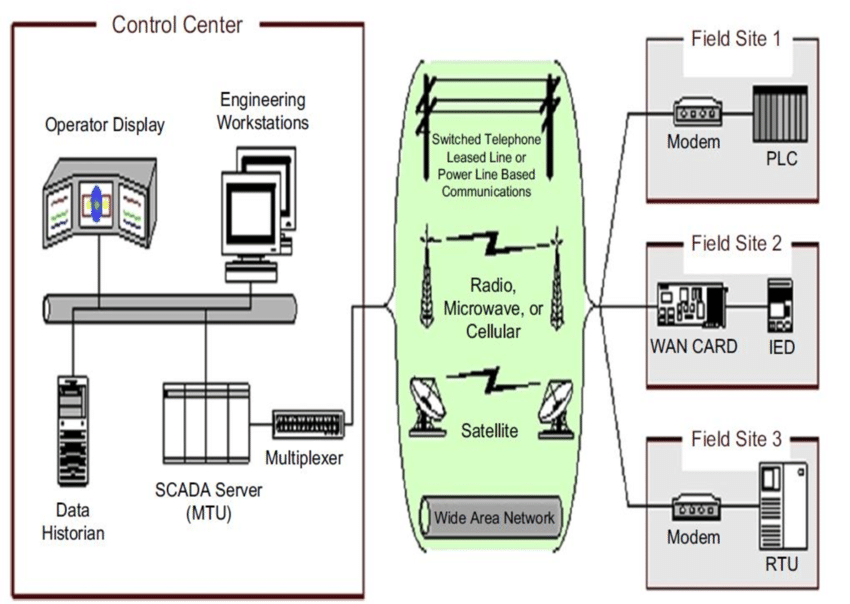
\includegraphics[width=0.8\textwidth]{scada_communication.png}
    \caption{SCADA System general layout communication system \autocite{nist_sp800_82}.}
    \label{fig:scada_communication}
\end{figure*}

Substations provide process information from field devices, which can be pre-processed and aggregated before transmission. Messages, measurements, and counts are timestamped and archived in the SCADA database. 

\subsection{Phasor Measurement Units}\label{subsec:ch1/sec2/sub2}

Phasors are complex numbers that represent the magnitude $X_m$  and phase angle $\varphi$ of a sinusoidal signal:
\begin{equation}
    x(t)=X_m \cos (\omega t+\varphi),
    % x(t)=\hat{x} \cos (\omega t+\varphi)
    \label{eq:phasor}
\end{equation}
as equivalent synchrophasor representation of the waveform:
\begin{equation}
    \begin{aligned}
X & =\left(X_{\mathrm{m}} / \sqrt{2}\right) \mathrm{e}^{\mathrm{j} \varphi} \\
& =\left(X_{\mathrm{m}} / \sqrt{2}\right)(\cos \varphi+\mathrm{j} \sin \varphi) \\
& =X_{\mathrm{r}}+\mathrm{j} X_{\mathrm{i}},
\end{aligned}
\end{equation}
where the magnitude is the rms value, $Xm /\sqrt{2}$, of the waveform and the subscripts $r$ and $i$ signify real and imaginary parts. The angle $\varphi$ is time-dependent, especially at $t = 0$. This phasor relates to angular frequency $\omega$; evaluations with other phasors must be done with the same time scale and frequency.

The required time synchronized phasor measurements are derived by PMUs, which are specialized devices that analyze the continuous analogue signals of AC voltage and current at a specific location in a power system and translate them into high-rate digital samples. Applying discrete Fourier transform, PMUs extract magnitude, phase, sequence, frequency, and rate of change of frequency (ROCOF), of the alternating signals given at its input terminal, as shown in Figure~\cref{fig:pmu_data}. Although PMU deployment is mainly in transmission systems, its use is increasingly expanding in distribution grids to improve observability \autocite{7779155}.

\nomenclature{\(ROCOF\)}{Rate of Change of Frequency}

\begin{figure*}[htbp]
    \centering
    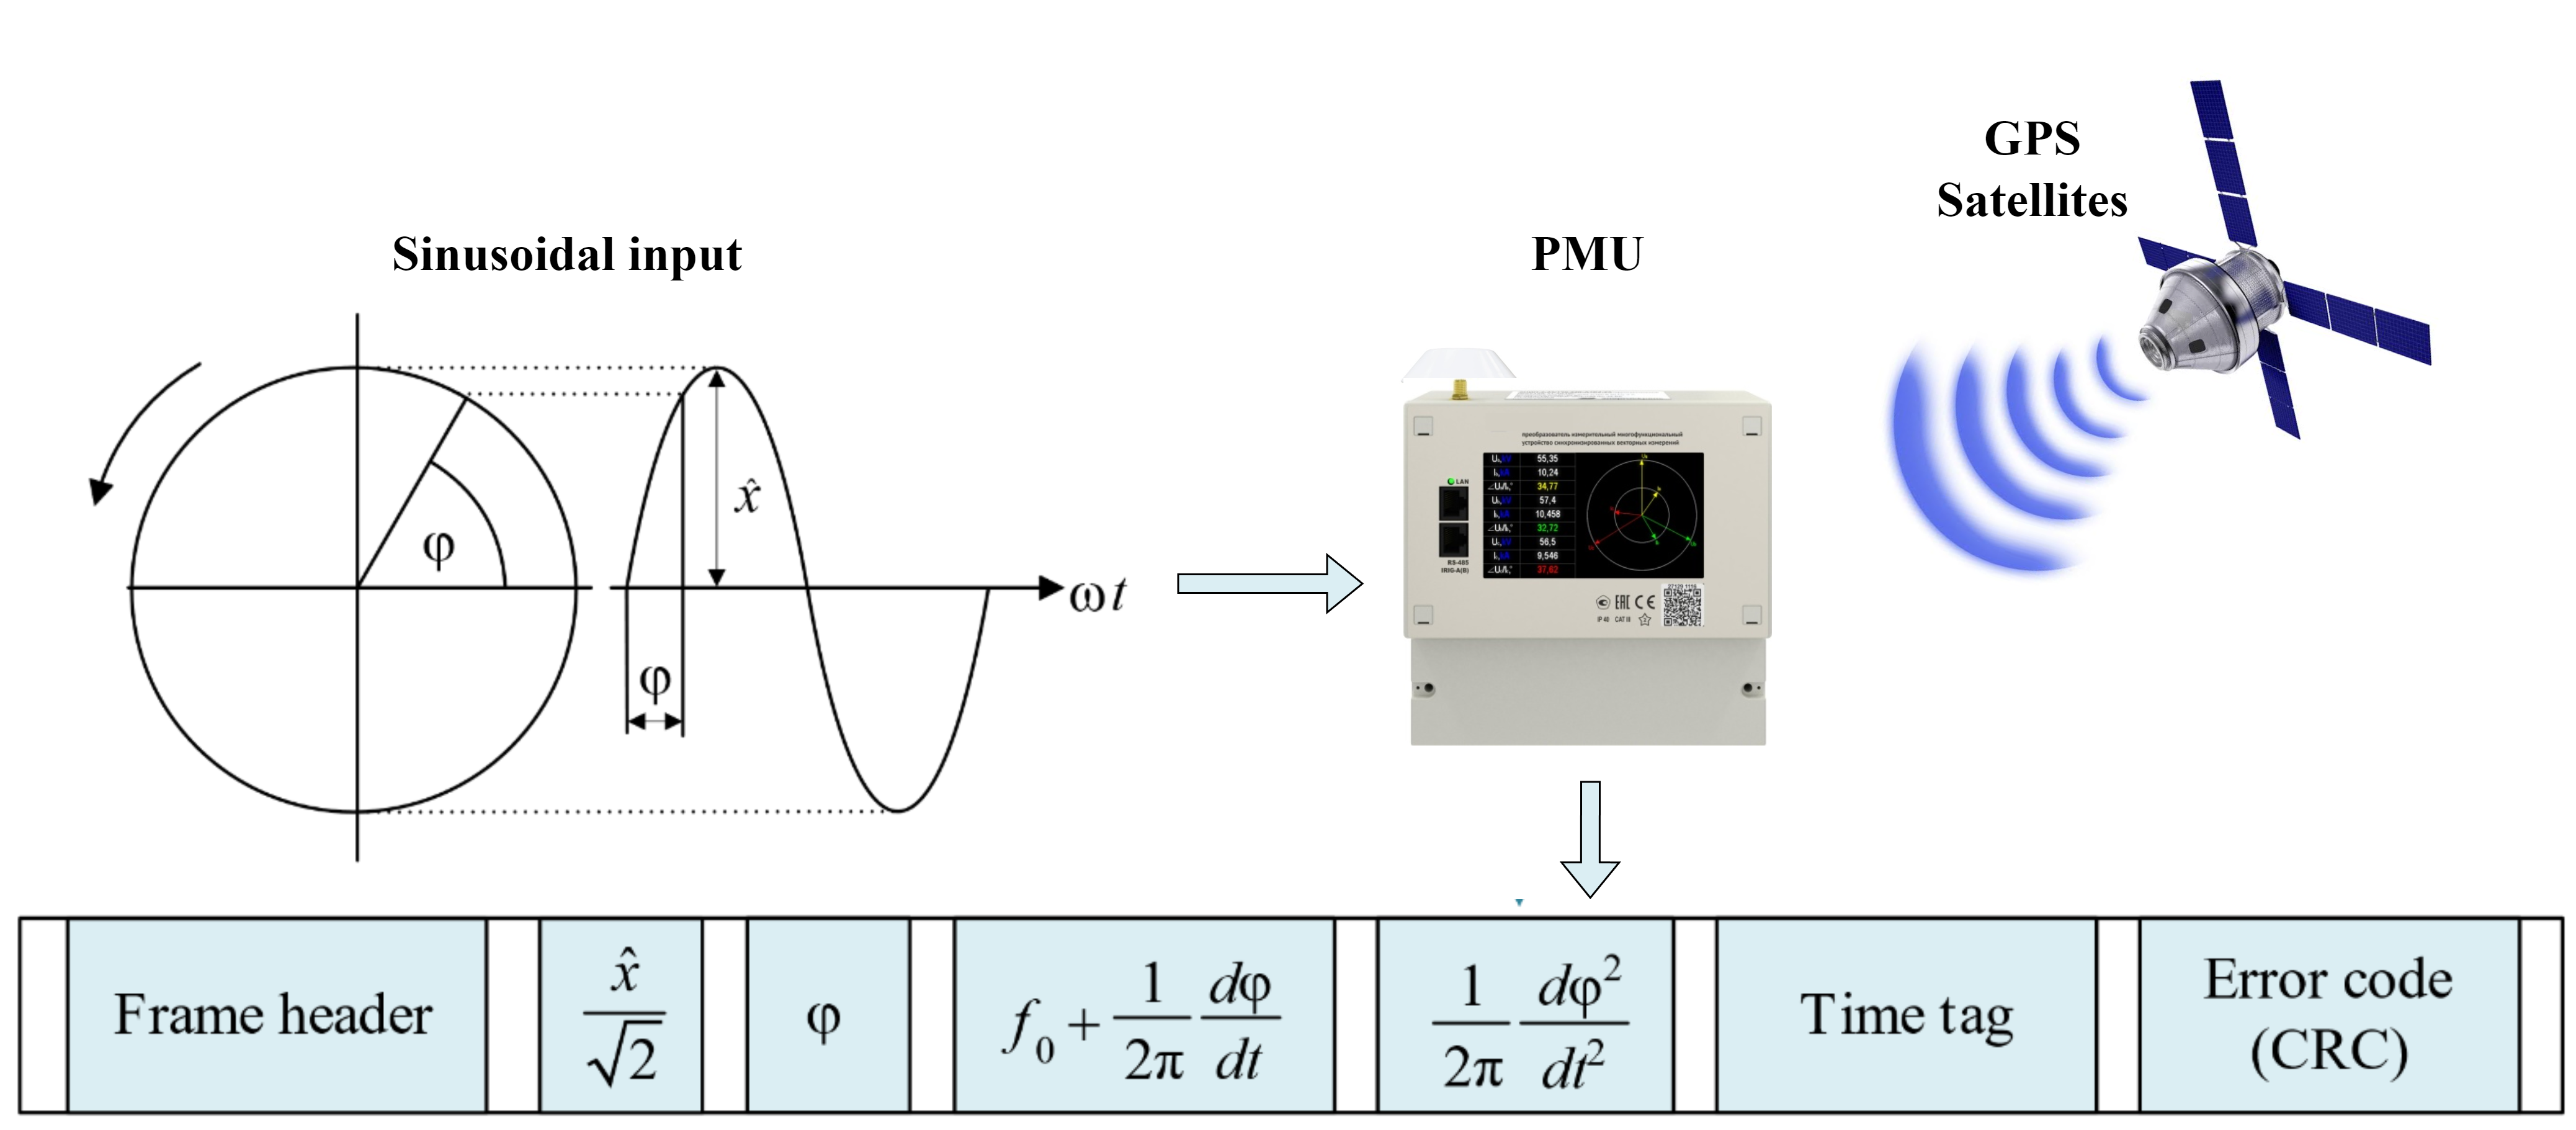
\includegraphics[width=1\textwidth]{pmu_data.png}
    \caption{The extraction of synchrophasor data packets in power systems.}
    \label{fig:pmu_data}
\end{figure*}

A PMU frame, in addition to measurement samples, includes a frame header with extra information such as cyclic redundancy check codes and measurement quality indicator \autocite{6111222}. A precise time source, such as Global Positioning System (GPS), provides the time signal to synchronize the measurements of various PMU devices.

Thanks to the precise time stamps provided by PMUs, applications for control, monitoring, and protection can access synchronized and comparable data streams in real time \autocite{5447627}. Commercial PMUs support a broad range of reporting rate, from 10 $reports/sec$ up to 240 $reports/sec$. The time tag accuracy requirement is $\pm1\mu s$, which corresponds to an angle error of 0.018 degrees for a 50 $Hz$ system.

\section{Power System State Estimation}\label{sec:ch1/sec3}

Due to the presence of noise, communication latency, missing measurements, and temporary communication failures, the raw telemetered data obtained from acquisition are often incomplete and have potential for errors. In practice, the measurements collected - such as bus voltage magnitudes, injected active and reactive power at buses, and power flows along branches - are inherently imperfect, affected by instrument inaccuracies, data conversion errors, communication noise, and occasional data corruption. Additionally, due to redundancy in measurement placement and sporadic data availability, the system may be partially unobservable at any given time.

To address these issues, state estimation algorithms are employed to:
\begin{itemize}
    \item Compensate for measurement noise and inaccuracies.
    \item Interpolate missing data.
    \item Detect and suppress bad data.
    \item Ensure observability in the presence of incomplete datasets.
    \item Generate a consistent and physically feasible system state.
\end{itemize}

To realize these functionality, the typical structural modules of SE is applied in diagram and presented in Figure~\cref{fig:se_flowchart}. To maintain an accurate system representation, the topology-processor \autocite{32475}, a specialized block within the state estimator, is continuously informed of any alterations in the network's structure and the most recent state assessments, allowing it to dynamically revise the network map. Based on this current topological understanding and the incoming stream of measurements, the system then performs an observability analysis to determine if the measurement set is rich enough to fully characterize the network's state. Only after the network's topology and its observability are adequately determined, the state estimator can proceed with its core task: calculating the optimal state vector from the available measurements and the underlying network model. 

\begin{figure*}[htbp]
    \centering
    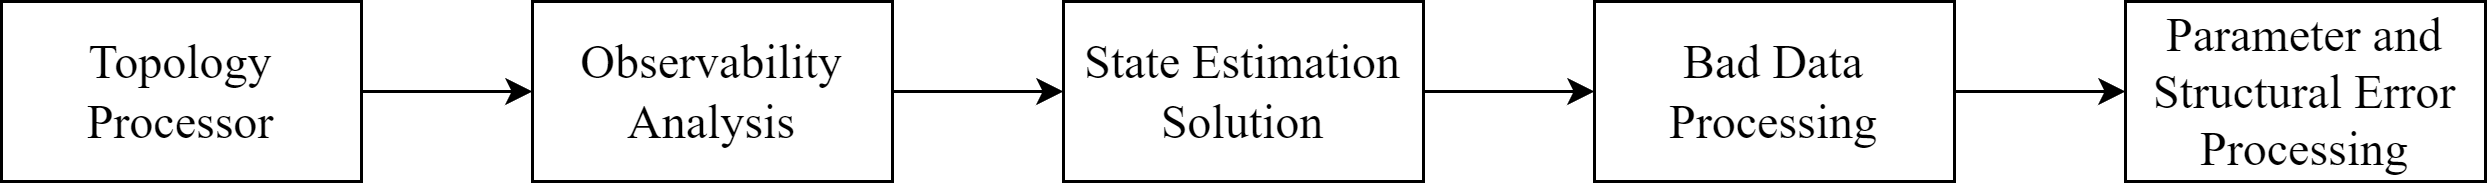
\includegraphics[width=1\textwidth]{se_flowchart.png}
    \caption{State Estimation functional modules.}
    \label{fig:se_flowchart}
\end{figure*}

Among the algorithmic part of SE the weighted least squares method has become a de facto standard to approximate a steady-state representation of the power system \autocite{abur2004power}. However, least squares SE algorithm is not very robust against  measurement outliers or large deviations \autocite{WU199080}, which caused such a factors as:
\begin{itemize}
    \item Sensor errors: Sensors may introduce measurement errors due to factors like manufacturing defects, environmental factors, and aging.
    \item Communication errors: Sensors transmit measurements to the state estimator through communication channels. Various factors, including channel noise, interference, and cyber-attacks, can cause errors in these transmitted measurements.
    \item Environmental factors: Environmental factors like temperature, humidity, and vibration can cause measurement errors.
    \item Human errors: Measurement inaccuracies can arise from human mistakes during sensor installation, calibration, and operation.
\end{itemize}

Thus, an essential next step is to apply thorough bad data detection and diagnostic procedures to identify inaccuracies in system parameters and the structural model. For doing that, a detailed database of electrical equipment characteristics and types for establishing a precise network model must be established. In addition, a covariance matrix with estimated measurement error variances is necessary.

Spreading of synchrophasor technology within PMUs gave an impetus to development of linear and hybrid state estimators evolved \autocite{1717598, BI20081343, 6878488}. In case of a high number of PMUs, the system could become completely observable. The direct measurement of the state variables on all buses allows a simple and fast linear SE solution \autocite{8620530}. The calculation time for large SE problems can be reduced by applying hierarchical or distributed SE schemes \autocite{7182780, 4162601}.

Due to the constantly evolving nature of power systems, it is essential to monitor their dynamic behavior in real time. This requires performing state estimation at short intervals. Traditional static state estimators fall short in accurately capturing these rapid changes, especially in PEDGs. To address this limitation, a technique known as Dynamic State Estimation (DSE) has been developed \autocite{1099844, 4074246}. DSE leverages a physical model that reflects the time-varying characteristics of the power system, enabling it to forecast the system's state at the next time step $(t+1)$ based on information from the current step $(t)$. One of the key benefits of DSE is its predictive capability, which allows for proactive decision-making. This forecasting feature significantly enhances the effectiveness of energy management system operations and control strategies.

\nomenclature{\(DSE\)}{Dynamic State Estimation}

To detect and identify issues like bad data, network reconfigurations, and abrupt state variations in DSE is suggested in \autocite{Nishiya1982}. Utilizing simple dynamic state vector models and linearized measurement equations, Kalman filtering theory is employed for estimation \autocite{Leite1983}, with one of the most widely used methods in power system DSE being the Extended Kalman Filter (EKF), which considers both the incoming measurements and the predicted state to obtain an optimal estimate of the system state, as mentioned in \autocite{Mandal1995}.

The study in \autocite{4510059} thoroughly examines the use of EKF to incorporate dynamic state variables, such as generator rotor speed and angle, into SE. This EKF-based process is validated on a multi-machine system under different disturbances. EKF-UI, an extension, is used in \autocite{5871327} for joint estimation of states and unknown inputs in synchronous machines. In \autocite{6024863}, a new distributed EKF framework is introduced, addressing the complexities of large-scale renewables and smart grids. This method enhances computational speed by dividing systems into subsystems for distributed implementation of DSE in extensive power networks.

The EKF, a commonly used estimation algorithm for nonlinear systems, faces challenges like implementation difficulty, tuning complexity, and limited reliability to nearly linear systems within update intervals \autocite{1271397}. To address EKF's issues due to linearization, the Unscented Transformation (UT) was developed to propagate mean and covariance through nonlinear transformations. The benefits of the Unscented Kalman Filter (UKF), rooted in UT, are discussed in literature \autocite{Valverde2011, 6019414, 6112697}. Studies \autocite{5619951, 6112697} confirm UKF's superior accuracy and easier application for generator dynamics with simulations. Analysis with three power systems demonstrates UKF's superior filtering over EKF in slower dynamic changes \autocite{Valverde2011}. UKF's effectiveness in estimating frequency, amplitude, and phase, even in noisy conditions, is shown in \autocite{6019414}. A non-derivative Kalman filtering approach for nonlinear systems control is explored in \autocite{5892889}, and a new state estimation method using UKF for power and frequency is detailed in \autocite{6142065}.

Though hybrid, linear, and DSE techniques are frequently explored in research, their adoption in operational EMS settings remains limited due to their strong reliance on dependable ICT \autocite{8624411}. Literature proposes algorithms to enhance DSE speed and robustness \autocite{7742899,WANG2020105390,8063917,7864445}, and for advanced uses like model predictive control \autocite{5342446, 6632979}, online DSA \autocite{SUN2016160, 6158623}, and wide area control \autocite{6202751}. However, detailed plans for the next-generation EMS and its future-proof architecture incorporating DSE for system operations are still lacking. The primary distinctions between SSE and DSE lie in their applications, modeling, and data needs. SSE is used for dispatching and monitoring voltage and flow limit breaches, while DSE is relevant to DSA and time-domain model calibration. Most power system DSE techniques employ Kalman filters, which typically rely on data streams from PMU-based WAMS \autocite{6802979,5871327,7501856,TEBIANIAN2015109}. General overviews of DSE algorithms and applications are found in \autocite{Simon_2006,Singh_Pal_2019}, with power system-specific DSE algorithms assessed in \autocite{6887334}. Table \ref{tab:se_comparison} compares the previously discussed state estimation methods.

% Please add the following required packages to your document preamble:
\begin{table}[]
\caption{Comparison of state estimation approaches}
\label{tab:se_comparison}
\resizebox{\textwidth}{!}{%
\begin{tabular}{|l|llll|}
\hline
\multicolumn{1}{|c|}{\multirow{2}{*}{\textbf{}}} & \multicolumn{4}{c|}{\textbf{State Estimation Type}} \\ \cline{2-5} 
\multicolumn{1}{|c|}{} & \multicolumn{1}{c|}{\textbf{Classic}} & \multicolumn{1}{c|}{\textbf{Hybrid}} & \multicolumn{1}{c|}{\textbf{Linear}} & \multicolumn{1}{c|}{\textbf{Dynamic}} \\ \hline
\textbf{\begin{tabular}[c]{@{}l@{}}Data \\ source\end{tabular}} & \multicolumn{1}{c|}{SCADA} & \multicolumn{1}{c|}{SCADA and PMU} & \multicolumn{1}{c|}{PMU} & \multicolumn{1}{c|}{PMU} \\ \hline
\textbf{\begin{tabular}[c]{@{}l@{}}Model \\ basis\end{tabular}} & \multicolumn{1}{c|}{\begin{tabular}[c]{@{}c@{}}Algebraic steady \\ state power flow\end{tabular}} & \multicolumn{1}{c|}{\begin{tabular}[c]{@{}c@{}}Algebraic steady \\ state power flow\end{tabular}} & \multicolumn{1}{c|}{\begin{tabular}[c]{@{}c@{}}Algebraic dynamic \\ power flow\end{tabular}} & \begin{tabular}[c]{@{}l@{}}Differential-algebraic \\ equation-based \\ time domain model\end{tabular} \\ \hline
\textbf{\begin{tabular}[c]{@{}l@{}}Input \\ data\end{tabular}} & \multicolumn{1}{l|}{\begin{tabular}[c]{@{}l@{}}Bus voltage \\ magnitudes: $U_{i,j}$;\\ Bus injections:  \\ $P_{i,j}, Q_{i,j}, I_{ij}$;\\ Branch admittance: \\ $Y = G_{ij},+jB_{ij}$;\end{tabular}} & \multicolumn{1}{l|}{\begin{tabular}[c]{@{}l@{}}Bus voltage \\ magnitudes $U_{i,j}$;\\ selected $U(t)$;\\ Bus injections  \\ $P_{i,j} Q_{i,j}$;\\ Branch flows \\ $P_{ij}, Q_{ij}, I_{ij}$;\\ Branch admittance  \\ $Y = G_{ij},+jB_{ij}$\end{tabular}} & \multicolumn{1}{l|}{\begin{tabular}[c]{@{}l@{}}Complex bus \\ voltages $U_{i,j}(t)$;\\ Branch admittance  \\ Y = $G_{ij},+jB_{ij}$\end{tabular}} & \begin{tabular}[c]{@{}l@{}}Complex bus \\ voltages $Ui,j(t)$; \\ Branch currents $I(t)$; \\ Parameter set \\ for equipment \\ and controller models\end{tabular} \\ \hline
\textbf{\begin{tabular}[c]{@{}l@{}}Resulting \\ state \\ variables\end{tabular}} & \multicolumn{1}{l|}{\begin{tabular}[c]{@{}l@{}}$U_{i,j}$, branch flows, \\ transformer tap \\ positions, \\ switching state \\ (corrected topology)\end{tabular}} & \multicolumn{1}{l|}{$U_{i,j}$, branch flows} & \multicolumn{1}{l|}{\begin{tabular}[c]{@{}l@{}}$U_{i,j}$, branch flows, \\ topology\end{tabular}} & \begin{tabular}[c]{@{}l@{}}Algebraic states: \\ {[}$z_1,...,z_n${]}, \\ differential states: \\ {[}$x_1,...,x_n${]},\\ and state derivatives: \\ {[}$\dot{x}_1,...,\dot{x}_n${]}\end{tabular} \\ \hline
\textbf{\begin{tabular}[c]{@{}l@{}}Complexity \\ and \\ computing \\ time\end{tabular}} & \multicolumn{1}{l|}{Medium} & \multicolumn{1}{l|}{Medium} & \multicolumn{1}{l|}{Low} & High \\ \hline
\textbf{\begin{tabular}[c]{@{}l@{}}Complexity \\ and \\ computing \\ time\end{tabular}} & \multicolumn{1}{l|}{Medium} & \multicolumn{1}{l|}{Medium} & \multicolumn{1}{l|}{Low} & High \\ \hline
\textbf{\begin{tabular}[c]{@{}l@{}}EMS \\ implementation\end{tabular}} & \multicolumn{1}{l|}{State of the art} & \multicolumn{1}{l|}{\begin{tabular}[c]{@{}l@{}}Some \\ implementations\end{tabular}} & \multicolumn{1}{l|}{Applied by WAMS} & \begin{tabular}[c]{@{}l@{}}Scarce implementations, \\ experimental state\end{tabular} \\ \hline
\end{tabular}%
}
\end{table}

\section{Static State Estimation}\label{sec:ch1/sec4}

Static state estimation (SSE) is defined as the process for determining the voltage magnitudes and angles of all buses in the power system at a given time, under the assumption of steady-state operation \autocite{Phadke12008springer}. This method is based on the quasi-static nature of power systems, where system changes are relatively slow compared to the SE time scale. It has served as a cornerstone of modern power network control systems since its introduction in the early 1970s by Schweppe and Handschin \autocite{4074022}. 

\subsubsection{Maximum likelihood method}

Maximum likelihood estimation (MLE) is a statistical technique used to estimate the parameters of a model by selecting the values that make the observed data most probable. The principle behind MLE is to identify the set of parameters that maximizes the likelihood function, which quantifies how well the model explains the measured data. In the context of power system state estimation, this involves modeling measurement errors, typically assumed to follow a normal distribution, and then deriving the parameter values that best align the model with the data. The likelihood function is based on the joint probability of the measurements given the state variables, and the estimation process seeks to find the state that maximizes this function. 

Measurement errors are typically assumed to follow a Normal distribution, characterized by two parameters: the mean $\mu$ and the variance $\sigma^2$. The normal probability density function (pdf) for a random variable $z$, with mean $\mu$, and standard deviation $\sigma$ can be defined as \autocite{Abur2004}:
\begin{equation}
    f(z)=\frac{1}{\sqrt{2 \pi} \sigma} \exp \left[-\frac{1}{2 \sigma^{2}}\left(z-\mu\right)^{2}\right]
\end{equation}

Taking into account the assumption based on considering m independent measurements and each having the same Gaussian pdf, and each measurement is assumed to be independent of the others, the joint pdf can be simply written as the product of individual pdfs. The resulting  product function $f_m(z)$ can be given by:
\begin{equation}
    f_{m}(z)=f\left(z_{1}\right) f\left(z_{2}\right) \ldots f\left(z_{m}\right)
\end{equation}

The function $f_m(z)$ is called the likelihood function for the set of $m$ measurements. It measures the probability of observing measurements in vector $z$. Maximum likelihood estimation of $f_m(z)$ involves maximizing it by varying parameters $\mu$ and $\sigma$ of the density function. This is simplified by maximizing the logarithm of the likelihood function, with its value given by function $f(z)$:
\begin{equation}
    \log f(z)=-\frac{1}{2} \frac{(z-\mu)^{2}}{\sigma}-\log \sigma \sqrt{2 \pi}
\end{equation}
or the modified function \(L=\log f_{m}(z)\).

\begin{equation}
    L=\sum_{i=1}^{m} \log f\left(z_{i}\right)=-\sum_{i=1}^{m} \log \sigma_{i}-\frac{m}{2} \log 2 \pi-\frac{1}{2} \sum_{i=1}^{m}\left(\frac{z_{i}-\mu_{i}}{\sigma_{i}}\right)^{2}
\end{equation}

The maximum likelihood estimate is obtained by finding the maximum of \(\log f_{m}(z)\), which can also be obtained by finding the minimum of 
\begin{equation}
    \min J(z)=\sum_{i=1}^{m}\left(\frac{z_{i}-\mu_{i}}{\sigma_{i}}\right)^{2}
\label{eq:wls_estimator}    
\end{equation}
which is known as \textit{weighted least squares} estimator.

The minimization problem can be rewritten, considering the form of residuals \(r_{i}=z_{i}-\mu_{i}\), if $r_i$ is residual of measurement $i$. Here, the mean $\mu_{i}$, which is the expected value of $z_{i}$, can be expressed as $h_i(x)$, a nonlinear function relating the system state vector $x$ to the $i$th measurement. Considering that the square of residual $r_i$ weighted by $W_i$ is equal to inverse of error variance $\sigma_{i}^2$, the minimization problem can also be written as

\begin{equation}
    \begin{array}{c}
    \operatorname{min} \quad \sum_{i=1}^{m} W_{i} r_{i}^{2} \\
    \text { s.t. } z_{i}=h_{i}(x)+r_{i}, i=1, \ldots, m
\end{array}
\label{eq:min_rsd}
\end{equation}

In case of matrix format of the above equations:
\begin{equation}
    \begin{array}{l}
\min J(x)=[z-h(x)]^{T} [z-h(x)] / R_{ii}
\end{array}
\end{equation}
where
\begin{equation}
    R=\left[\begin{array}{llll}
\sigma_{1}^{2} & & & \\
& \sigma_{2}^{2} & & \\
& & \ddots & \\
& & & \sigma_{m}^{2}
\end{array}\right]
\label{eq:mlm_r}
\end{equation}
where $[R]$ is the \textit{covariance matrix} of measurement errors.

To address this optimization problem, the solution is required to follow the first-order optimality condition, which:
\begin{equation}
    \frac{\partial J}{\partial x}=0 \quad \rightarrow \quad\left[-\frac{\partial h}{\partial x}\right]^{T} R^{-1}[z-h(x)]=0
    \label{eq:mlm_optcond}
\end{equation}
where \(H(x)=\delta h / \delta x\) is the Jacobian matrix of dimension (m × n) measurement.

As $h(x)$ in AC SE is nonlinear, Gauss-Newton method can be applied to linearize the function. Considering \(g(x)=\frac{\partial J}{\partial x}\) and expanding $g(x)$ around the state vector $x^k$ the following iterative procedure can be obtained:
\begin{equation}
    h(x+\Delta x) \approx h(x)+H(x) \Delta x
\end{equation}

\begin{equation}
    x^{k+1}=x^{k}-\left[G\left(x^{k}\right)\right]^{-1} g\left(x^{k}\right)
\end{equation}

\begin{equation}
    G\left(x^{k}\right)=\frac{\partial g\left(x^{k}\right)}{\partial x}=H^{T}\left(x^{k}\right) R^{-1} H\left(x^{k}\right)
\end{equation}

\begin{equation}
    g\left(x^{k}\right)=-H^{T}\left(x^{k}\right) R^{-1}\left(z-h\left(x^{k}\right)\right.
\end{equation}
where symmetric matrix \(H^{T}\left(x^{k}\right) R^{-1} H\left(x^{k}\right)=G(x)\) is  called the gain matrix, $k$ is the iteration index, $x^k$ is the solution vector at iteration $k$.

\subsubsection{Network topology}
The implementation of SE requires detailed information about network topology and parameters. The component model that represents the entire network presented by: tap changing and phase shifting transformer, transmission line (TL), shunt capacitors or reactors and loads with generators.  

\paragraph{Transmission line}
% To characterize the transmission line two port $\pi$-model is using. The power system is considered to be in balanced steady state operation. This requires that transmission lines are completely transposed, bus loads and branch power flows remain three-phase and balanced, and all series or shunt devices are symmetrical across the three phases. 

A two port $\pi$-model is utilized to characterize the positive sequence of the TL. It is assumed that the power system is operating in steady state mode and under balanced condition. This requires that all TLs are fully transposed, all bus loads and branch power flows will be three phase and balanced,  and all other series or shunt devices will be symmetrical in the three phases. The transmission line with a positive sequence series impedance of \(R + jX\) and total line charging susceptance of $j2B$ can be presented as equivalent circuit presented, shown in Figure~\cref{fig:pi_model}.

\begin{figure}[htbp]
    \centering
    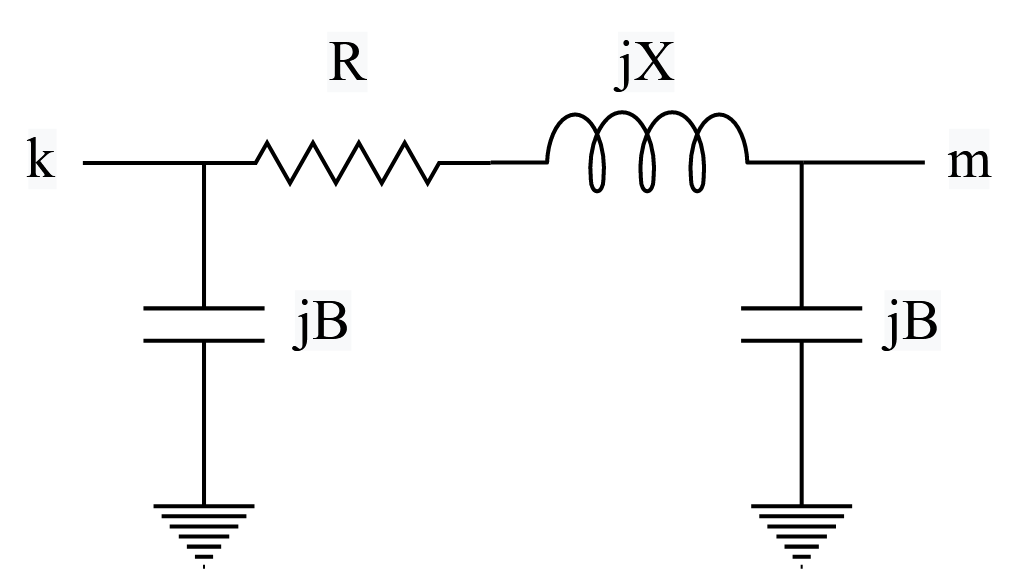
\includegraphics[width=0.45\linewidth]{graphics/pi_model.png}
    \caption{Two port $\pi$-model equivalent circuit of TL}
    \label{fig:pi_model}
\end{figure}

\paragraph{Tap Changing Transformer}

Transformers can be modeled as ideal transformer in series with resistance and inductance, with terminal buses $m$ and $k$ on impedance side and the tap side bus respectively, as shown in Figure~\cref{fig:tf_eqc}.

\begin{figure}[htbp]
    \centering
    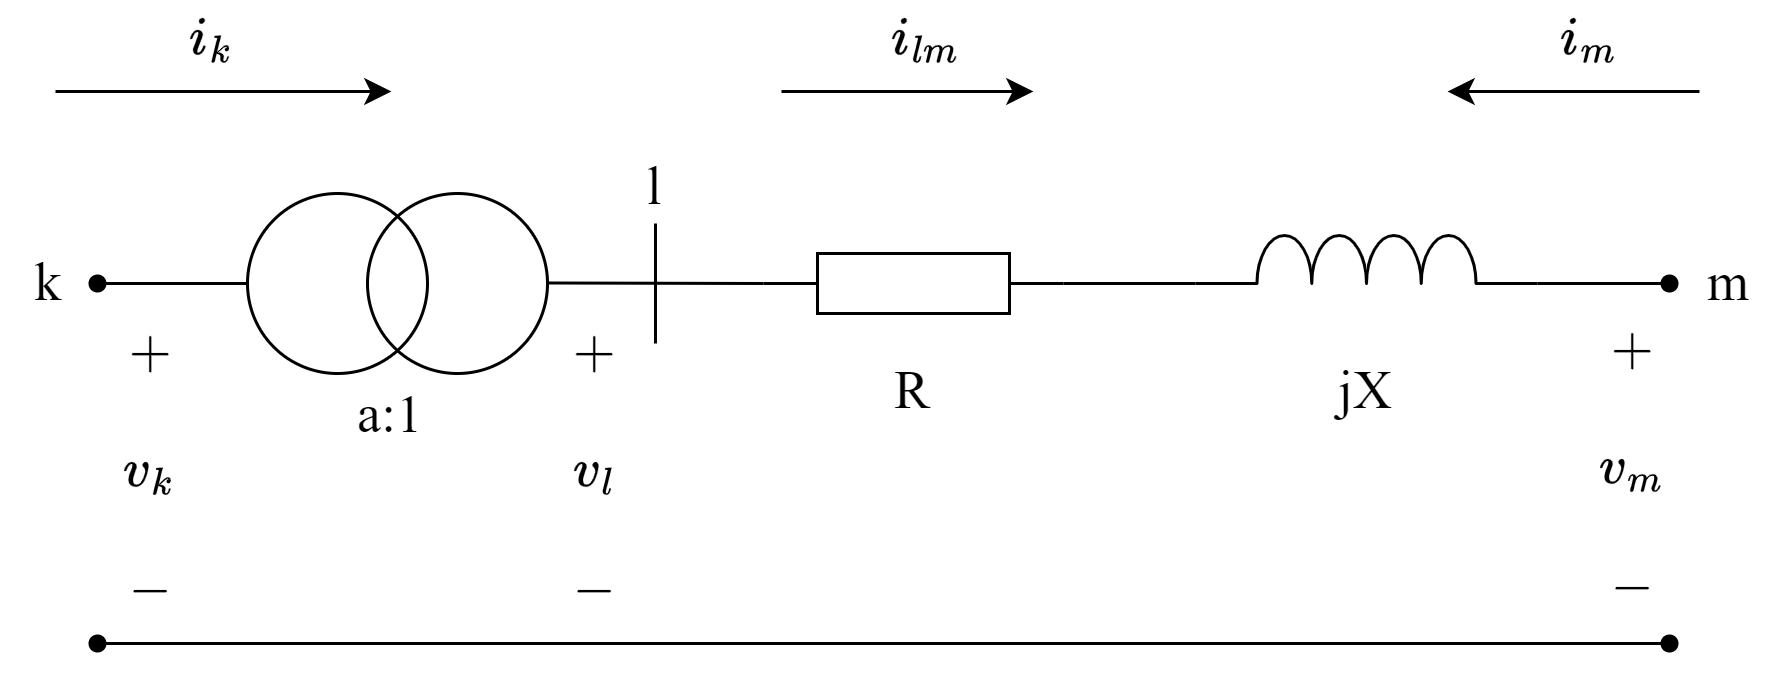
\includegraphics[width=0.8\linewidth]{graphics/TF_EQC.png}
    \caption{Two port $\pi$-model equivalent circuit of TL}
    \label{fig:tf_eqc}
\end{figure}

The nodal equations for the two-port circuit in Figure~\cref{fig:tf_eqc} are obtained by expressing the currents $i_{lm}$ and $i_{m}$ at the ends of the series branch \(R+jX\). If $y$ is the branch admittance \(l-m\), the terminal current injections are described by:
\begin{equation}
    \left[\begin{array}{c}
i_{\ell m} \\
i_{m}
\end{array}\right]=\left[\begin{array}{rr}
y & -y \\
-y & y
\end{array}\right]\left[\begin{array}{c}
v_{\ell} \\
v_{m}
\end{array}\right]
\end{equation}
Substituting for \(i_{lm} = a \cdot i_{k}\) and \(v_{l} = v_{k}/a\), the following form will be obtained:
\begin{equation}
    \left[\begin{array}{c}
i_{k} \\
i_{m}
\end{array}\right]=\left[\begin{array}{rr}
y / a^{2} & -y / a \\
-y / a & y
\end{array}\right]\left[\begin{array}{c}
v_{k} \\
v_{m}
\end{array}\right]
\end{equation}
where $a$ is the in phase tap ratio.

\paragraph{Shunt Capacitors or Reactors}
To manage voltage or reactive power, installing shunt capacitors or reactors is an option. The sign of the susceptance indicates the type: negative for capacitors and positive for reactors.

\paragraph{Loads and Generators}
Power injections from loads and generators, expressed as complex power, remain independent of the network model. In contrast, constant impedance loads are accounted for as shunt admittances at respective buses.

\paragraph{Network Modeling}
Mentioned component models are utilized to construct a complete power system model. This involves formulating equations for each node based on Kirchhoff's current law, as follows:
\begin{equation}
    I=\left[\begin{array}{c}
i_{1} \\
i_{2} \\
\vdots \\
i_{N}
\end{array}\right]=\left[\begin{array}{cccc}
Y_{11} & Y_{12} & \cdots & Y_{1 N} \\
Y_{21} & Y_{22} & \cdots & Y_{2 N} \\
\vdots & \vdots & \vdots & \vdots \\
Y_{N 1} & Y_{N 2} & \cdots & Y_{N N}
\end{array}\right]\left[\begin{array}{c}
v_{1} \\
v_{2} \\
\vdots \\
v_{N}
\end{array}\right]=Y \cdot V
\end{equation}
where \\ 
$I$ is the net current injection phasors vector\\
$V$ is the bus voltage phasors vector\\  
$Y_{km}$ is the ($k,m$)th element of the $Y$ matrix\\ 
$N$ is the number of bus\\
$i_k$ is the current injection phasor in bus $k$\\
$v_k$ is the voltage at bus $k$

\paragraph{Measurement Model}
The SE of the power system usually involves measurements such as line power flows, bus power injections, and bus voltage magnitudes, represented using either rectangular or polar coordinates. For a system of $N$ buses, the state vector in polar coordinates includes \(2N-1\) elements: $N$ for voltage magnitudes and \(N-1\) for phase angles, setting the reference bus's angle at 0. Using bus 1 as reference, the state vector $x$ is structured as follows:
\begin{equation}
    x^{T}=\left[\begin{array}{llllllll}
\theta_{2} & \theta_{3} & \ldots & \theta_{N} & V_{1} & V_{2} & \ldots & V_{N}
\end{array}\right]
\end{equation}

For a general two-port $\pi$ model applied to network branches, the real and reactive power injected at bus i, denoted as $P_i$ and $Q_i$, respectively, are:
\begin{equation}
    P_{i}=V_{i} \sum_{j=1}^{N} V_{j}\left(G_{i j} \cos \left(\theta_{i j}\right)+B_{i j} \sin \left(\theta_{i j}\right)\right)
\end{equation}
\begin{equation}
    Q_{i}=V_{i} \sum_{j=1}^{N} V_{j}\left(G_{i j} \sin \left(\theta_{i j}\right)-B_{i j} \cos \left(\theta_{i j}\right)\right)
\end{equation}
Real and reactive power flow from bus $i$ to bus $j$:
\begin{equation}
    P_{i j}=V_{i}^{2}\left(g_{s i}+g_{i j}\right)-V_{i} V_{j}\left(g_{i j} \cos \left(\theta_{i j}\right)+b_{i j} \sin \left(\theta_{i j}\right)\right)
\end{equation}
\begin{equation}
    Q_{i j}=-V_{i}^{2}\left(b_{s i}+b_{i j}\right)-V_{i} V_{j}\left(g_{i j} \sin \left(\theta_{i j}\right)-b_{i j} \cos \left(\theta_{i j}\right)\right)
\end{equation}
where $V_i$ and $\theta_i$ is the voltage magnitude and phase angle at bus $i$; \(\theta_{ij} = \theta_i-\theta_j\);  \(G_{ij}+jB_{ij}\) is the $ij$th element of the complex bus admittance matrix; \(g_{ij}+jb_{ij}\) is the admittance of the series branch connecting buses $i$ and $j$; \(g_{si}+jb_{si}\) is the admittance of the shunt branch connected at bus $i$.

\subsubsection{Weighted least squares method}

The Weighted Least Squares (WLS) method is widely used for state estimation in power systems, minimizing the weighted squared differences between measurements and estimates. Weights give priority to certain measurements. Here are the steps for using WLS in power system state estimation:
\begin{itemize}
    \item Initialize the state vector to an initial guess (flat start).
    \item Calculate the gain matrix, Jacobian matrix, and measurement vector.
    \item Calculate the weighted sum of the squared residuals.
    \item Update the state vector.
    \item Repeat steps until the state vector converges.
\end{itemize}

In the WLS method, the necessary condition to minimize the performance index is given in \ref{eq:mlm_optcond}  as \(-H^{T}(x) R^{-1}[z-h(x)]=0\). Here $H$, the  Jacobian matrix, can be written as
\begin{equation}
H = 
\left[
\begin{array}{cc}
\frac{\partial P_i}{\partial \theta} & \frac{\partial P_i}{\partial V} \\
\frac{\partial P_{ij}}{\partial \theta} & \frac{\partial P_{ij}}{\partial V} \\
\frac{\partial Q_i}{\partial \theta} & \frac{\partial Q_i}{\partial V} \\
\frac{\partial Q_{ij}}{\partial \theta} & \frac{\partial Q_{ij}}{\partial V} \\
\frac{\partial V_i}{\partial \theta} & \frac{\partial V_i}{\partial V}
\end{array}
\right]
\end{equation}

The matrix represented as the diagonal covariance matrix for the measurements referenced in \ref{eq:mlm_r}. This equation shows that weights are determined by the inverse of the measurement variances. Consequently, a lower variance in high-quality measurements results in higher weights.

Detecting and identifying incorrect data is an essential role of SE software due to the relatively common occurrence of measurement failures in large and expansive power systems \autocite{WU199080}.

% It should be noted that the traditional least squares SE algorithm is not very robust against measurement outliers or large deviations \autocite{WU199080}, bad data detection routines are required. A prerequisite for an effective estimation of the system state is a properly maintained database of electrical equipment characteristics and type-related parameters to set up an accurate network model. Furthermore, a covariance matrix is required that contains the approximated variances of measurement error.

\subsubsection{Bad data}

If normalized measurement residuals are normally distributed, their squared sum follows a $\chi^2$ distribution. Within the WLS SSE framework, the $\chi^2$-test combined with the LNR test is commonly used for bad data detection (BDD) and identification of BD’s origin. BDD by the $\chi^2$-test steps are given as follows \autocite{gomez2017electric}: 
\begin{itemize}
    \item Solve SE problem and compute the objective function \autocite{7232283}:
        \begin{equation}
            J_{B D D}(\hat{\boldsymbol{x}})=\sum_{i=1}^{m} \frac{\left[z_{i}-h_{i}(\hat{\boldsymbol{x}})\right]^{2}}{\Omega_{i i}}=\sum_{i=1}^{m} \frac{r_{i}^{2}}{\Omega_{i i}}
        \end{equation}
        where $z_i$ is $i$-th measurement, $h_i$ is $i$-th equation from set $h$ of measurement  equations, and $\Omega_{ii}$ is the variance of  the $i$-th measurement residual, $\Omega$ is the residual covariance matrix.
        
    \item From the $\chi^2$ distribution table identify the value corresponding to $p$ probability and \((m-n)\) degrees of freedom \autocite{abur2004power}.

    \item In case of \(J_{B D D}(\hat{\boldsymbol{x}}) \geq \chi^2_{(m-n),\rho}\), then BD is present with confidence probability level of $\rho$ and \((m-n)\) degrees of freedom; otherwise, there is no BD.

    \item If BD is detected, calculate normalized residual for each measurement, $r^{Norm}_i$, as:
        \begin{equation}
        r_{i}^{\text {Norm }}=\frac{\left|z_{i}-h_{i}(\hat{\boldsymbol{x}})\right|}{\sqrt{\Omega_{i i}}}=\frac{\left|r_{i}\right|}{\sqrt{\Omega_{i i}}}
        \end{equation}

    \item If $r^{Norm}_i$ is the largest normalized residual, meets or exceeds the threshold $\tau$, then the $i$-th measurement will be suspected as BD. For normalized residuals following Standard Gaussian distribution, threshold $\tau$ can be selected as \(\tau = 3\).

\end{itemize}

\subsubsection{Sudden load/generation change}
Abrupt changes in the power system's state can occur due to sudden load changes (SLC) or sudden generation changes (SGC). Significant SLC often results from major shifts in industrial loads or the connection/disconnection of substantial load sections. While past research has extensively covered SLC, the rise of uncertain renewable energy sources has introduced SGC as a new challenge \autocite{Nishiya_1982}.

It should be noted that the $\chi^2$ test carried out on the residuals of the measurements obtained through WLS SSE is unable to detect  SLC/SGC. However, application of forecasting-aided state estimation (FASE) can be helpful for the detection of these events due to the advantages that the state transition model brings.

% \subsubsection{SSE modifications}
% The evolution of linear and hybrid state estimators has progressed with the advancement of synchrophasor technology and deployment of PMUs \autocite{Tomashevich2019}. Given a certain level of observability by PMUs, using complex bus and branch currents rather than active and reactive branch flows allows for quick linear SE techniques \autocite{8620530}. For large SE problems, employing hierarchical or distributed SE schemes can decrease calculation time \autocite{4162601}. 

% Distributed state estimation involves estimating a system's state through measurements from numerous sensors distributed across the system. Compared to traditional centralized approaches, distributed state estimation provides key benefits: greater scalability for large systems, increased resilience against sensor failures and communication interruptions, and real-time state estimation capabilities.

\subsubsection{Matrix splitting} 

In order to obtain the solution of the SE problem in a distributed manner, the matrix splitting method can be used and after doing a certain number of iterations the answer converges to the centralized solution \autocite{7171105}. The main equation for matrix splitting for a problem of \(Ax = y\) is:
\begin{equation}
    x^{t+1}=M^{-1} N x^{t}+M^{-1} y
    \label{eq:ms_maineq}
\end{equation}
that $A$ can be decomposed into the sum of an invertible (or diagonal) matrix $M$, and a matrix $N$; so that we have \(M = D+E^{'}_{ii}\) and \(N = E-E^{'}_{ii}\). Here, $D$ comprises the diagonal elements of $A$, while $E$ contains the off-diagonal elements. Furthermore, $E^{'}_{ii}$ is a specific diagonal matrix defined as follows:
\begin{equation}
    E_{i i}^{\prime}=\alpha \sum_{j=1}^{n}\left|E_{i j}\right|.
\end{equation}

It should be noted that \ref{eq:ms_maineq} converges if the spectral radius of the \(M-1N\) matrix is less than 1 \((\rho(M-1N) < 1)\). Using \ref{eq:ms_maineq} iteratively leads to convergence to the system \(Ax = y\) final solution.

% that we have assumed \(\alpha = 1\) for simplicity. 
\subsubsection{ADMM} 
To solve distributed SE another method has been introduced in \autocite{6340375}, which is based on alternating direction method of multipliers (ADMM) \autocite{boyd2004convex}. ADMM enhances the performance of current SE solvers and ensures convergence to the centralized solution, even without local observability.

In general, the distributed SE problem can be formulated as:
\begin{equation}
    \begin{array}{c}
\min _{x_{k}} \sum_{k=1}^{K} H_{k}\left(x_{k}\right) \\
\mathrm{x}_{k}[l]=x_{l}[k], \forall l \in N_{k}, \forall k \in K
\end{array}
\end{equation}
where $N_k$ denotes the set of regions sharing states with area $k$ and $x_{k,l}$ is auxiliary variable introduced per pair of interacting areas $k$, $l$.

The constraint forces neighboring areas to consent on their shared variables. Augmented Lagrangian function is as follows:
\begin{equation}
    \begin{array}{c}
L\left(\left\{x_{k}\right\},\left\{x_{k l}\right\} ;\left\{v_{k l}\right\}\right) \\
:=\sum_{k=1}^{K}\left[H_{k}\left(x_{k}\right)+\sum_{l \in N_{k}}\left(v_{k, l}^{T}\left(x_{k[l]}-x_{k l}\right)+\frac{c}{2}\left\|x_{k[l]}-x_{k l}\right\|_{2}^{2}\right)\right]
\end{array}
\end{equation}
where $v_{k,l}$ is Lagrangian multiplier and \(c > 0\).

\begin{equation}
    \begin{aligned}
\left\{\mathrm{x}_{k}^{t+1}\right\} & :=\arg \min L\left(\left\{x_{k}\right\},\left\{x_{k l}^{t}\right\} ;\left\{v_{k l}^{t}\right\}\right) \\
\left\{\mathrm{x}_{k l}^{t+1}\right\} & :=\arg \min L\left(\left\{x_{k}^{t+1}\right\},\left\{x_{k l}\right\} ;\left\{v_{k l}^{t}\right\}\right) \\
v_{k, l}^{t+1} & :=v_{k, l}^{t}+c\left(x_{k[l]}^{t+1}-x_{k l}^{t+1}\right), \forall k
\end{aligned}
\end{equation}


\subsection{Dynamic State Estimation}

Dynamic state estimation algorithms determine the system's dynamic states, which are the state variables in the power system's nonlinear algebraic equations. The initial step in DSE is identifying the mathematical model for the power system's temporal behavior. Utilizing this model and measurement data, DSE forecasts the next dynamic state vector.

A dynamic system is typically represented by a set of non-linear differential equations \autocite{4510059, 5871327}:
\begin{equation}
    \frac{d x}{d t}=f(x, u, w)
    \label{eq:dynamic_eq}
\end{equation}
where $f(.)$ is the system function, $x$ vector represents the state variables, the $u$ vector represents the algebraic variables and $w$ stands for process (system) noise. It can be rewritten in discrete form as:
\begin{equation}
    \begin{aligned}
x_{k} & =x_{k-1}+f\left(x_{k-1}, u_{k-1}, w_{k-1}\right) \Delta t \\
& =g\left(x_{k-1}, u_{k-1}, w_{k-1}\right)
\end{aligned}
\end{equation}
where $x$ is the state vector composed of $n = 2N-1$ elements (bus voltages and  phase angles at all buses except phase angle at the slack bus), $k-1$ is the present instant of time index, $k$ is the next instant of time index  and $\Delta t$ is the time step.

The set of $m$ measurements, usually composed of active and reactive power flows, active and reactive power injections, and voltage magnitudes, can be represented as a vector of non-linear functions $h(.)$ in terms of the state variables $x$ and the measurement noise $v$ as below:
\begin{equation}
    z_{k}=h\left(x_{k}, v_{k}\right)
\end{equation}
The resulting error between the measured and calculated values is given by
\begin{equation}
    \epsilon_{k}=z_{k}-h\left(x_{k}, v_{k}\right)
\end{equation}

In power systems, measurement functions are inherently nonlinear. To handle a nonlinear model, the EKF, which linearizes through Taylor series, can be used \autocite{Jin_2021}. Other Kalman filter variants for nonlinear systems include the UKF \autocite{Valverde2011}, Particle Filter \autocite{DELMORAL1997653}, iterated EKF \autocite{BRETAS198970}, Ensemble Kalman Filter \autocite{Houtekamer_Mitchell_1998}, Second-order Kalman Filter \autocite{Nash_Gelb_Kasper_1974}, and Cubature Kalman Filter \autocite{BASETTI2022100712}.

\subsubsection{Extended Kalman Filter (EKF) Algorithm}

The Extended Kalman Filter prediction-correction method can be summarized as \autocite{Simon_2006}:
\begin{enumerate}
    \item The discrete time system equations are presented as follows:
    \begin{equation}
    \begin{aligned}
        x_{k} & =f_{k-1}\left(x_{k-1}, u_{k-1}, w_{k-1}\right) \\
        y_{k} & =h_{k}\left(x_{k}, v_{k}\right) \\
        w_{k} & \sim\left(0, Q_{k}\right) \\
        v_{k} & \sim\left(0, R_{k}\right)
    \end{aligned}
    \end{equation}  
where the system noise covariance matrix is represented by $Q_k$ and the measurement noise covariance matrix is represented by $R_k$.
    \item Initialize the filter:
    \begin{equation}
        \begin{aligned}
        \hat{x}_{0}^{+} & =E\left(x_{0}\right) \\
        P_{0}^{+} & =E\left[\left(x-\hat{x}_{0}^{+}\right)\left(x-\hat{x}_{0}^{+}\right)^{T}\right]
        \end{aligned}
    \end{equation}
    where ${x}_{0}^{+}$ represents the initial state and $P_{0}^{+}$ denotes the initial state covariance  matrix. The subscript $+$ indicates an a posteriori estimate.
    
    % After, for $k = 1, 2, ...$, perform the following:

    \item Compute the following partial derivative matrices at the current state estimate ${x}_{k-1}^{+}$:
        \begin{equation}
        \begin{aligned}
            F_{k-1} & =\left.\frac{\partial f_{k-1}}{\partial x}\right|_{\hat{x}_{k-1}^{+}} \\
            L_{k-1} & =\left.\frac{\partial f_{k-1}}{\partial w}\right|_{\hat{x}_{k-1}^{+}}
        \end{aligned}
        \end{equation}
    
    \item Perform the time update of state estimate and estimation-error covariance matrix:
        \begin{equation}
        \begin{aligned}
            P_{k}^{-} & =F_{k-1} P_{k-1}^{+} F_{k-1}^{T}+L_{k-1} Q_{k-1}^{+} L_{k-1}^{T} \\
            \hat{x}_{k}^{-} & =f_{k-1}\left(\hat{x}_{k-1}^{+}, u_{k-1}, 0\right)
        \end{aligned}
        \end{equation}
    where the subscript $-$ denotes the estimate is in an a priori estimate.
    
    \item Perform the following partial derivative matrices at the state update ${x}_{k}^{-}$:
        \begin{equation}
        \begin{aligned}
        H_{k} & =\left.\frac{\partial h_{k}}{\partial x}\right|_{\hat{x}_{k}^{-}} \\
        V_{k} & =\left.\frac{\partial h_{k}}{\partial v}\right|_{\hat{x}_{k}^{-}}
        \end{aligned}
        \end{equation}

    \item Update the state estimate and estimation covariance with the measurement as follows:
        \begin{equation}
        \begin{aligned}
        K_{k} & =P_{k}^{-} H_{k}^{T}\left(H_{k} P_{k}^{-} H_{k}^{T}+V_{k} R_{k} V_{k}^{T}\right)^{-1} \\
        \hat{x}_{k}^{+} & =\hat{x}_{k}^{-}+K_{k}\left[y_{k}-h_{k}\left(\hat{x}_{k}^{-}, 0\right)\right] \\
        P_{k}^{+} & =\left(I-K_{k} H_{k}\right) P_{k}^{-}
        \end{aligned}
        \end{equation}
    where $K_k$ is the Kalman gain matrix, ${x}_{k}^{-}$ is the state estimate and $P_{k}^{+}$ is the estimation error covariance matrix.
        
\end{enumerate}













% Сошлёмся на библиографию.
% Одна ссылка: \autocite[с.~54]{Sokolov}\autocite[с.~36]{Gaidaenko}.
% Две ссылки: \autocite{Sokolov,Gaidaenko}.
% Ссылка на собственные работы: \autocite{vakbib1, confbib2}.
% Много ссылок: %\autocite[с.~54]{Lermontov,Management,Borozda} % такой «фокус»
% %вызывает biblatex warning относительно опции sortcites, потому что неясно, к
% %какому источнику относится уточнение о страницах, а bibtex об этой проблеме
% %даже не предупреждает
% \autocite{Lermontov, Management, Borozda, Marketing, Constitution, FamilyCode,
%     Gost.7.0.53, Razumovski, Lagkueva, Pokrovski, Methodology, Berestova,
%     Kriger}%
% \ifnumequal{\value{bibliosel}}{0}{% Примеры для bibtex8
%     \autocite{Sirotko, Lukina, Encyclopedia, Nasirova}%
% }{% Примеры для biblatex через движок biber
%     \autocite{Sirotko2, Lukina2, Encyclopedia2, Nasirova2}%
% }%
% .
% И~ещё немного ссылок:~\autocite{Article,Book,Booklet,Conference,Inbook,Incollection,Manual,Mastersthesis,
%     Misc,Phdthesis,Proceedings,Techreport,Unpublished}
% % Следует обратить внимание, что пробел после запятой внутри \autocite{}
% % обрабатывается ожидаемо, а пробел перед запятой, может вызывать проблемы при
% % обработке ссылок.
% \autocite{medvedev2006jelektronnye, CEAT:CEAT581, doi:10.1080/01932691.2010.513279,
%     Gosele1999161,Li2007StressAnalysis, Shoji199895, test:eisner-sample,
%     test:eisner-sample-shorted, AB_patent_Pomerantz_1968, iofis_patent1960}%
% \ifnumequal{\value{bibliosel}}{0}{% Примеры для bibtex8
% }{% Примеры для biblatex через движок biber
%     \autocite{patent2h, patent3h, patent2}%
% }%
% .

% \ifnumequal{\value{bibliosel}}{0}{% Примеры для bibtex8
% Попытка реализовать несколько ссылок на конкретные страницы
% для \texttt{bibtex} реализации библиографии:
% [\autocitenum{Sokolov}, с.~54; \autocitenum{Gaidaenko}, с.~36].
% }{% Примеры для biblatex через движок biber
% Несколько источников (мультицитата):
% % Тут специально написано по-разному тире, для демонстрации, что
% % применение специальных тире в настоящий момент в biblatex приводит к непоказу
% % "с.".
% \autocites[vii--x, 5, 7]{Sokolov}[v"--~x, 25, 526]{Gaidaenko}[vii--x, 5, 7]{Techreport},
% работает только в \texttt{biblatex} реализации библиографии.
% }%

% Ссылки на собственные работы:~\autocite{vakbib1, confbib1}.

% Сошлёмся на приложения: Приложение~\cref{app:A}, Приложение~\cref{app:B2}.

% Сошлёмся на формулу: формула~\cref{eq:equation1}.

% Сошлёмся на изображение: рисунок~\cref{fig:knuth}.

% Стандартной практикой является добавление к ссылкам префикса, характеризующего тип элемента.
% Это не является строгим требованием, но~позволяет лучше ориентироваться в документах большого размера.
% Например, для ссылок на~рисунки используется префикс \textit{fig},
% для ссылки на~таблицу "--- \textit{tab}.

% В таблице \cref{tab:tab_pref} приложения~\cref{app:B4} приведён список рекомендуемых
% к использованию стандартных префиксов.

% В некоторых ситуациях возникает необходимость отойти от требований ГОСТ по оформлению ссылок на
% литературу.
% В таком случае можно воспользоваться дополнительными опциями пакета \verb+biblatex+.

% Например, в ссылке на книгу~\autocite{sobenin_kdv} использование опции \verb+maxnames=4+ позволяет
% вывести имена всех четырёх авторов.
% По ГОСТ имена последних трёх авторов опускаются.

% Кроме того, часто возникают проблемы с транслитерованными инициалами. Некоторые буквы русского
% алфавита по правилам транслитерации записываются двумя буквами латинского алфавита (ю-yu, ё-yo и
% т.д.).
% Такие инициалы \verb+biblatex+ будет сокращать до одной буквы, что неверно.
% Поправить его работу можно использовав опцию \verb+giveninits=false+.
% Пример использования этой опции можно видеть в ссылке~\autocite{initials}.

% \section{Формулы}\label{sec:ch1/sec3}

% Благодаря пакету \textit{icomma}, \LaTeX~одинаково хорошо воспринимает
% в~качестве десятичного разделителя и запятую (\(3,1415\)), и точку (\(3.1415\)).

% \subsection{Ненумерованные одиночные формулы}\label{subsec:ch1/sec3/sub1}

% Вот так может выглядеть формула, которую необходимо вставить в~строку
% по~тексту: \(x \approx \sin x\) при \(x \to 0\).

% А вот так выглядит ненумерованная отдельностоящая формула c подстрочными
% и надстрочными индексами:
% \[
%     (x_1+x_2)^2 = x_1^2 + 2 x_1 x_2 + x_2^2
% \]

% Формула с неопределенным интегралом:
% \[
%     \int f(\alpha+x)=\sum\beta
% \]

% При использовании дробей формулы могут получаться очень высокие:
% \[
%     \frac{1}{\sqrt{2}+
%         \displaystyle\frac{1}{\sqrt{2}+
%             \displaystyle\frac{1}{\sqrt{2}+\cdots}}}
% \]

% В формулах можно использовать греческие буквы:
% %Все \original... команды заранее, ради этого примера, определены в Dissertation\userstyles.tex
% \[
%     \alpha\beta\gamma\delta\originalepsilon\epsilon\zeta\eta\theta%
%     \vartheta\iota\kappa\varkappa\lambda\mu\nu\xi\pi\varpi\rho\varrho%
%     \sigma\varsigma\tau\upsilon\originalphi\phi\chi\psi\omega\Gamma\Delta%
%     \Theta\Lambda\Xi\Pi\Sigma\Upsilon\Phi\Psi\Omega
% \]
% \[%https://texfaq.org/FAQ-boldgreek
%     \boldsymbol{\alpha\beta\gamma\delta\originalepsilon\epsilon\zeta\eta%
%         \theta\vartheta\iota\kappa\varkappa\lambda\mu\nu\xi\pi\varpi\rho%
%         \varrho\sigma\varsigma\tau\upsilon\originalphi\phi\chi\psi\omega\Gamma%
%         \Delta\Theta\Lambda\Xi\Pi\Sigma\Upsilon\Phi\Psi\Omega}
% \]

% Для добавления формул можно использовать пары \verb+$+\dots\verb+$+ и \verb+$$+\dots\verb+$$+,
% но~они считаются устаревшими.
% Лучше использовать их функциональные аналоги \verb+\(+\dots\verb+\)+ и \verb+\[+\dots\verb+\]+.

% \subsection{Ненумерованные многострочные формулы}\label{subsec:ch1/sec3/sub2}

% Вот так можно написать две формулы, не нумеруя их, чтобы знаки <<равно>> были
% строго друг под другом:
% \begin{align}
%     f_W & =  \min \left( 1, \max \left( 0, \frac{W_{soil} / W_{max}}{W_{crit}} \right)  \right), \nonumber \\
%     f_T & =  \min \left( 1, \max \left( 0, \frac{T_s / T_{melt}}{T_{crit}} \right)  \right), \nonumber
% \end{align}

% Выровнять систему ещё и по переменной \( x \) можно, используя окружение
% \verb|alignedat| из пакета \verb|amsmath|. Вот так:
% \[
% |x| = \left\{
% \begin{alignedat}{2}
%      &   & x, \quad & \text{eсли } x\geqslant 0 \\
%      & - & x, \quad & \text{eсли } x<0
% \end{alignedat}
% \right.
% \]
% Здесь первый амперсанд (в исходном \LaTeX\ описании формулы) означает
% выравнивание по~левому краю, второй "--- по~\( x \), а~третий "--- по~слову
% <<если>>. Команда \verb|\quad| делает большой горизонтальный пробел.

% Ещё вариант:
% \[
%     |x|=
%     \begin{cases}
%         \phantom{-}x, \text{если } x \geqslant 0 \\
%         -x, \text{если } x<0
%     \end{cases}
% \]

% Кроме того, для  нумерованных формул \verb|alignedat| делает вертикальное
% выравнивание номера формулы по центру формулы. Например, выравнивание
% компонент вектора:
% \begin{equation}
%     \label{eq:2p3}
%     \begin{alignedat}{2}
%         {\mathbf{N}}_{o1n}^{(j)} = \,{\sin} \phi\,n\!\left(n+1\right)
%         {\sin}\theta\,
%         \pi_n\!\left({\cos} \theta\right)
%         \frac{
%         z_n^{(j)}\!\left( \rho \right)
%         }{\rho}\,
%          & {\boldsymbol{\hat{\mathrm e}}}_{r}\,+      \\
%         +\,
%         {\sin} \phi\,
%         \tau_n\!\left({\cos} \theta\right)
%         \frac{
%         \left[\rho z_n^{(j)}\!\left( \rho \right)\right]^{\prime}
%         }{\rho}\,
%          & {\boldsymbol{\hat{\mathrm e}}}_{\theta}\,+ \\
%         +\,
%         {\cos} \phi\,
%         \pi_n\!\left({\cos} \theta\right)
%         \frac{
%         \left[\rho z_n^{(j)}\!\left( \rho \right)\right]^{\prime}
%         }{\rho}\,
%          & {\boldsymbol{\hat{\mathrm e}}}_{\phi}\:.
%     \end{alignedat}
% \end{equation}

% Ещё об отступах. Иногда для лучшей <<читаемости>> формул полезно
% немного исправить стандартные интервалы \LaTeX\ с учётом логической
% структуры самой формулы. Например в формуле~\cref{eq:2p3} добавлен
% небольшой отступ \verb+\,+ между основными сомножителями, ниже
% результат применения всех вариантов отступа:
% \begin{align*}
%     \backslash!             & \quad f(x) = x^2\! +3x\! +2         \\
%     \mbox{по-умолчанию}     & \quad f(x) = x^2+3x+2               \\
%     \backslash,             & \quad f(x) = x^2\, +3x\, +2         \\
%     \backslash{:}           & \quad f(x) = x^2\: +3x\: +2         \\
%     \backslash;             & \quad f(x) = x^2\; +3x\; +2         \\
%     \backslash \mbox{space} & \quad f(x) = x^2\ +3x\ +2           \\
%     \backslash \mbox{quad}  & \quad f(x) = x^2\quad +3x\quad +2   \\
%     \backslash \mbox{qquad} & \quad f(x) = x^2\qquad +3x\qquad +2
% \end{align*}

% Можно использовать разные математические алфавиты:
% \begin{align}
%     \mathcal{ABCDEFGHIJKLMNOPQRSTUVWXYZ} \nonumber  \\
%     \mathfrak{ABCDEFGHIJKLMNOPQRSTUVWXYZ} \nonumber \\
%     \mathbb{ABCDEFGHIJKLMNOPQRSTUVWXYZ} \nonumber
% \end{align}

% Посмотрим на систему уравнений на примере аттрактора Лоренца:

% \[
% \left\{
% \begin{array}{rl}
%     \dot x = & \sigma (y-x)  \\
%     \dot y = & x (r - z) - y \\
%     \dot z = & xy - bz
% \end{array}
% \right.
% \]

% А для вёрстки матриц удобно использовать многоточия:
% \[
%     \left(
%         \begin{array}{ccc}
%             a_{11} & \ldots & a_{1n} \\
%             \vdots & \ddots & \vdots \\
%             a_{n1} & \ldots & a_{nn} \\
%         \end{array}
%     \right)
% \]

% \subsection{Нумерованные формулы}\label{subsec:ch1/sec3/sub3}

% А вот так пишется нумерованная формула:
% \begin{equation}
%     \label{eq:equation1}
%     e = \lim_{n \to \infty} \left( 1+\frac{1}{n} \right) ^n
% \end{equation}

% Нумерованных формул может быть несколько:
% \begin{equation}
%     \label{eq:equation2}
%     \lim_{n \to \infty} \sum_{k=1}^n \frac{1}{k^2} = \frac{\pi^2}{6}
% \end{equation}

% Впоследствии на формулы~\cref{eq:equation1, eq:equation2} можно ссылаться.

% Сделать так, чтобы номер формулы стоял напротив средней строки, можно,
% используя окружение \verb|multlined| (пакет \verb|mathtools|) вместо
% \verb|multline| внутри окружения \verb|equation|. Вот так:
% \begin{equation} % \tag{S} % tag - вписывает свой текст
%     \label{eq:equation3}
%     \begin{multlined}
%         1+ 2+3+4+5+6+7+\dots + \\
%         + 50+51+52+53+54+55+56+57 + \dots + \\
%         + 96+97+98+99+100=5050
%     \end{multlined}
% \end{equation}

% Уравнения~\cref{eq:subeq_1,eq:subeq_2} демонстрируют возможности
% окружения \verb|subequations| (пакет \verb|amsmath|).
% \begin{subequations}
%     \label{eq:subeq_1}
%     \begin{gather}
%         y = x^2 + 1 \label{eq:subeq_1-1} \\
%         y = 2 x^2 - x + 1 \label{eq:subeq_1-2}
%     \end{gather}
% \end{subequations}
% Ссылки на отдельные уравнения~\cref{eq:subeq_1-1,eq:subeq_1-2,eq:subeq_2-1}.
% \begin{subequations}
%     \label{eq:subeq_2}
%     \begin{align}
%         y & = x^3 + x^2 + x + 1 \label{eq:subeq_2-1} \\
%         y & = x^2
%     \end{align}
% \end{subequations}

% \subsection{Форматирование чисел и размерностей величин}\label{sec:units}

% Числа форматируются при помощи команды \verb|\num|:
% \num{5,3};
% \num{2,3e8};
% \num{12345,67890};
% \num{2,6 d4};
% \num{1+-2i};
% \num{.3e45};
% \num[exponent-base=2]{5 e64};
% \num[exponent-base=2,exponent-to-prefix]{5 e64};
% \num{1.654 x 2.34 x 3.430}
% \num{1 2 x 3 / 4}.
% Для написания последовательности чисел можно использовать команды \verb|\numlist| и \verb|\numrange|:
% \numlist{10;30;50;70}; \numrange{10}{30}.
% Значения углов можно форматировать при помощи команды \verb|\ang|:
% \ang{2.67};
% \ang{30,3};
% \ang{-1;;};
% \ang{;-2;};
% \ang{;;-3};
% \ang{300;10;1}.

% Обратите внимание, что ГОСТ запрещает использование знака <<->> для обозначения отрицательных чисел
% за исключением формул, таблиц и~рисунков.
% Вместо него следует использовать слово <<минус>>.

% Размерности можно записывать при помощи команд \verb|\si| и \verb|\SI|:
% \si{\farad\squared\lumen\candela};
% \si{\joule\per\mole\per\kelvin};
% \si[per-mode = symbol-or-fraction]{\joule\per\mole\per\kelvin};
% \si{\metre\per\second\squared};
% \SI{0.10(5)}{\neper};
% \SI{1.2-3i e5}{\joule\per\mole\per\kelvin};
% \SIlist{1;2;3;4}{\tesla};
% \SIrange{50}{100}{\volt}.
% Список единиц измерений приведён в таблицах~\cref{tab:unit:base,
%     tab:unit:derived,tab:unit:accepted,tab:unit:physical,tab:unit:other}.
% Приставки единиц приведены в~таблице~\cref{tab:unit:prefix}.

% С дополнительными опциями форматирования можно ознакомиться в~описании пакета \texttt{siunitx};
% изменить или добавить единицы измерений можно в~файле \texttt{siunitx.cfg}.

% \begin{table}
%     \centering
%     \captionsetup{justification=centering} % выравнивание подписи по-центру
%     \caption{Основные величины СИ}\label{tab:unit:base}
%     \begin{tabular}{llc}
%         \toprule
%         Название  & Команда          & Символ         \\
%         \midrule
%         Ампер     & \verb|\ampere|   & \si{\ampere}   \\
%         Кандела   & \verb|\candela|  & \si{\candela}  \\
%         Кельвин   & \verb|\kelvin|   & \si{\kelvin}   \\
%         Килограмм & \verb|\kilogram| & \si{\kilogram} \\
%         Метр      & \verb|\metre|    & \si{\metre}    \\
%         Моль      & \verb|\mole|     & \si{\mole}     \\
%         Секунда   & \verb|\second|   & \si{\second}   \\
%         \bottomrule
%     \end{tabular}
% \end{table}

% \begin{table}
%     \small
%     \centering
%     \begin{threeparttable}% выравнивание подписи по границам таблицы
%         \caption{Производные единицы СИ}\label{tab:unit:derived}
%         \begin{tabular}{llc|llc}
%             \toprule
%             Название       & Команда               & Символ              & Название & Команда & Символ \\
%             \midrule
%             Беккерель      & \verb|\becquerel|     & \si{\becquerel}     &
%             Ньютон         & \verb|\newton|        & \si{\newton}                                      \\
%             Градус Цельсия & \verb|\degreeCelsius| & \si{\degreeCelsius} &
%             Ом             & \verb|\ohm|           & \si{\ohm}                                         \\
%             Кулон          & \verb|\coulomb|       & \si{\coulomb}       &
%             Паскаль        & \verb|\pascal|        & \si{\pascal}                                      \\
%             Фарад          & \verb|\farad|         & \si{\farad}         &
%             Радиан         & \verb|\radian|        & \si{\radian}                                      \\
%             Грей           & \verb|\gray|          & \si{\gray}          &
%             Сименс         & \verb|\siemens|       & \si{\siemens}                                     \\
%             Герц           & \verb|\hertz|         & \si{\hertz}         &
%             Зиверт         & \verb|\sievert|       & \si{\sievert}                                     \\
%             Генри          & \verb|\henry|         & \si{\henry}         &
%             Стерадиан      & \verb|\steradian|     & \si{\steradian}                                   \\
%             Джоуль         & \verb|\joule|         & \si{\joule}         &
%             Тесла          & \verb|\tesla|         & \si{\tesla}                                       \\
%             Катал          & \verb|\katal|         & \si{\katal}         &
%             Вольт          & \verb|\volt|          & \si{\volt}                                        \\
%             Люмен          & \verb|\lumen|         & \si{\lumen}         &
%             Ватт           & \verb|\watt|          & \si{\watt}                                        \\
%             Люкс           & \verb|\lux|           & \si{\lux}           &
%             Вебер          & \verb|\weber|         & \si{\weber}                                       \\
%             \bottomrule
%         \end{tabular}
%     \end{threeparttable}
% \end{table}

% \begin{table}
%     \centering
%     \begin{threeparttable}% выравнивание подписи по границам таблицы
%         \caption{Внесистемные единицы}\label{tab:unit:accepted}

%         \begin{tabular}{llc}
%             \toprule
%             Название        & Команда           & Символ          \\
%             \midrule
%             День            & \verb|\day|       & \si{\day}       \\
%             Градус          & \verb|\degree|    & \si{\degree}    \\
%             Гектар          & \verb|\hectare|   & \si{\hectare}   \\
%             Час             & \verb|\hour|      & \si{\hour}      \\
%             Литр            & \verb|\litre|     & \si{\litre}     \\
%             Угловая минута  & \verb|\arcminute| & \si{\arcminute} \\
%             Угловая секунда & \verb|\arcsecond| & \si{\arcsecond} \\ %
%             Минута          & \verb|\minute|    & \si{\minute}    \\
%             Тонна           & \verb|\tonne|     & \si{\tonne}     \\
%             \bottomrule
%         \end{tabular}
%     \end{threeparttable}
% \end{table}

% \begin{table}
%     \centering
%     \captionsetup{justification=centering}
%     \caption{Внесистемные единицы, получаемые из эксперимента}\label{tab:unit:physical}
%     \begin{tabular}{llc}
%         \toprule
%         Название                & Команда                  & Символ                 \\
%         \midrule
%         Астрономическая единица & \verb|\astronomicalunit| & \si{\astronomicalunit} \\
%         Атомная единица массы   & \verb|\atomicmassunit|   & \si{\atomicmassunit}   \\
%         Боровский радиус        & \verb|\bohr|             & \si{\bohr}             \\
%         Скорость света          & \verb|\clight|           & \si{\clight}           \\
%         Дальтон                 & \verb|\dalton|           & \si{\dalton}           \\
%         Масса электрона         & \verb|\electronmass|     & \si{\electronmass}     \\
%         Электрон Вольт          & \verb|\electronvolt|     & \si{\electronvolt}     \\
%         Элементарный заряд      & \verb|\elementarycharge| & \si{\elementarycharge} \\
%         Энергия Хартри          & \verb|\hartree|          & \si{\hartree}          \\
%         Постоянная Планка       & \verb|\planckbar|        & \si{\planckbar}        \\
%         \bottomrule
%     \end{tabular}
% \end{table}

% \begin{table}
%     \centering
%     \begin{threeparttable}% выравнивание подписи по границам таблицы
%         \caption{Другие внесистемные единицы}\label{tab:unit:other}
%         \begin{tabular}{llc}
%             \toprule
%             Название                  & Команда              & Символ             \\
%             \midrule
%             Ангстрем                  & \verb|\angstrom|     & \si{\angstrom}     \\
%             Бар                       & \verb|\bar|          & \si{\bar}          \\
%             Барн                      & \verb|\barn|         & \si{\barn}         \\
%             Бел                       & \verb|\bel|          & \si{\bel}          \\
%             Децибел                   & \verb|\decibel|      & \si{\decibel}      \\
%             Узел                      & \verb|\knot|         & \si{\knot}         \\
%             Миллиметр ртутного столба & \verb|\mmHg|         & \si{\mmHg}         \\
%             Морская миля              & \verb|\nauticalmile| & \si{\nauticalmile} \\
%             Непер                     & \verb|\neper|        & \si{\neper}        \\
%             \bottomrule
%         \end{tabular}
%     \end{threeparttable}
% \end{table}

% \begin{table}
%     \small
%     \centering
%     \begin{threeparttable}% выравнивание подписи по границам таблицы
%         \caption{Приставки СИ}\label{tab:unit:prefix}
%         \begin{tabular}{llcc|llcc}
%             \toprule
%             Приставка & Команда       & Символ      & Степень      &
%             Приставка & Команда       & Символ      & Степень        \\
%             \midrule
%             Иокто     & \verb|\yocto| & \si{\yocto} & \textminus24 &
%             Дека      & \verb|\deca|  & \si{\deca}  & 1              \\
%             Зепто     & \verb|\zepto| & \si{\zepto} & \textminus21 &
%             Гекто     & \verb|\hecto| & \si{\hecto} & 2              \\
%             Атто      & \verb|\atto|  & \si{\atto}  & \textminus18 &
%             Кило      & \verb|\kilo|  & \si{\kilo}  & 3              \\
%             Фемто     & \verb|\femto| & \si{\femto} & \textminus15 &
%             Мега      & \verb|\mega|  & \si{\mega}  & 6              \\
%             Пико      & \verb|\pico|  & \si{\pico}  & \textminus12 &
%             Гига      & \verb|\giga|  & \si{\giga}  & 9              \\
%             Нано      & \verb|\nano|  & \si{\nano}  & \textminus9  &
%             Терра     & \verb|\tera|  & \si{\tera}  & 12             \\
%             Микро     & \verb|\micro| & \si{\micro} & \textminus6  &
%             Пета      & \verb|\peta|  & \si{\peta}  & 15             \\
%             Милли     & \verb|\milli| & \si{\milli} & \textminus3  &
%             Екса      & \verb|\exa|   & \si{\exa}   & 18             \\
%             Санти     & \verb|\centi| & \si{\centi} & \textminus2  &
%             Зетта     & \verb|\zetta| & \si{\zetta} & 21             \\
%             Деци      & \verb|\deci|  & \si{\deci}  & \textminus1  &
%             Иотта     & \verb|\yotta| & \si{\yotta} & 24             \\
%             \bottomrule
%         \end{tabular}
%     \end{threeparttable}
% \end{table}

% \subsection{Заголовки с формулами: \texorpdfstring{\(a^2 + b^2 = c^2\)}{%
%         a\texttwosuperior\ + b\texttwosuperior\ = c\texttwosuperior},
%     \texorpdfstring{\(\left\vert\textrm{{Im}}\Sigma\left(
%             \protect\varepsilon\right)\right\vert\approx const\)}{|ImΣ (ε)| ≈ const},
%     \texorpdfstring{\(\sigma_{xx}^{(1)}\)}{σ\_\{xx\}\textasciicircum\{(1)\}}
% }\label{subsec:with_math}

% Пакет \texttt{hyperref} берёт текст для закладок в pdf-файле из~аргументов
% команд типа \verb|\section|, которые могут содержать математические формулы,
% а~также изменения цвета текста или шрифта, которые не отображаются в~закладках.
% Чтобы использование формул в заголовках не вызывало в~логе компиляции появление
% предупреждений типа <<\texttt{Token not allowed in~a~PDF string
%     (Unicode):(hyperref) removing...}>>, следует использовать конструкцию
% \verb|\texorpdfstring{}{}|, где в~первых фигурных скобках указывается
% формула, а~во~вторых "--- запись формулы для закладок.

% \section{Рецензирование текста}\label{sec:markup}

% В шаблоне для диссертации и автореферата заданы команды рецензирования.
% Они видны при компиляции шаблона в режиме черновика или при установке
% соответствующей настройки (\verb+showmarkup+) в~файле \verb+common/setup.tex+.

% Команда \verb+\todo+ отмечает текст красным цветом.
% \todo{Например, так.}

% Команда \verb+\note+ позволяет выбрать цвет текста.
% \note{Чёрный, } \note[red]{красный, } \note[green]{зелёный, }
% \note[blue]{синий.} \note[orange]{Обратите внимание на ширину и расстановку
%     формирующихся пробелов, в~результате приведённой записи (зависит также
%     от~применяемого компилятора).}

% Окружение \verb+commentbox+ также позволяет выбрать цвет.

% \begin{commentbox}[red]
%     Красный текст.

%     Несколько параграфов красного текста.
% \end{commentbox}

% \begin{commentbox}[blue]
%     Синяя формула.

%     \begin{equation}
%         \alpha + \beta = \gamma
%     \end{equation}
% \end{commentbox}

% \verb+commentbox+ позволяет закомментировать участок кода в~режиме чистовика.
% Чтобы убрать кусок кода для всех режимов, можно использовать окружение
% \verb+comment+.

% \begin{comment}
% Этот текст всегда скрыт.
% \end{comment}

% \section{Работа со списком сокращений и~условных обозначений}\label{sec:acronyms}

% С помощью пакета \texttt{nomencl} можно создавать удобный сортированный список
% сокращений и условных обозначений во время написания текста. Вызов
% \verb+\nomenclature+ добавляет нужный символ или сокращение с~описанием
% в~список, который затем печатается вызовом \verb+\printnomenclature+
% в~соответствующем разделе.
% Для того, чтобы эти операции прошли, потребуется дополнительный вызов
% \verb+makeindex -s nomencl.ist -o %.nls %.nlo+ в~командной строке, где вместо
% \verb+%+ следует подставить имя главного файла проекта (\verb+dissertation+
% для этого шаблона).
% Затем потребуется один или два дополнительных вызова компилятора проекта.
% \begin{equation}
%     \omega = c k,
% \end{equation}
% где \( \omega \) "--- частота света, \( c \) "--- скорость света, \( k \) "---
% модуль волнового вектора.
% \nomenclature{\(\omega\)}{частота света\nomrefeq}
% \nomenclature{\(c\)}{скорость света\nomrefpage}
% \nomenclature{\(k\)}{модуль волнового вектора\nomrefeqpage}
% Использование
% \begin{verbatim}
% \nomenclature{\(\omega\)}{частота света\nomrefeq}
% \nomenclature{\(c\)}{скорость света\nomrefpage}
% \nomenclature{\(k\)}{модуль волнового вектора\nomrefeqpage}
% \end{verbatim}
% после уравнения добавит в список условных обозначений три записи.
% Ссылки \verb+\nomrefeq+ на последнее уравнение, \verb+\nomrefpage+ "--- на
% страницу, \verb+\nomrefeqpage+ "--- сразу на~последнее уравнение и~на~страницу,
% можно опускать и~не~использовать.

% Группировкой и сортировкой пунктов в списке можно управлять с~помощью указания
% дополнительных аргументов к команде \verb+nomenclature+.
% Например, при вызове
% \begin{verbatim}
% \nomenclature[03]{\( \hbar \)}{постоянная Планка}
% \nomenclature[01]{\( G \)}{гравитационная постоянная}
% \end{verbatim}
% \( G \) будет стоять в списке выше, чем \( \hbar \).
% Для корректных вертикальных отступов между строками в описании лучше
% не~использовать многострочные формулы в~списке обозначений.

% \nomenclature{%
%     \( \begin{rcases}
%         a_n \\
%         b_n
%     \end{rcases} \)%
% }{коэффициенты разложения Ми в дальнем поле соответствующие электрическим и
%     магнитным мультиполям}
% \nomenclature[a\( e \)]{\( {\boldsymbol{\hat{\mathrm e}}} \)}{единичный вектор}
% \nomenclature{\( E_0 \)}{амплитуда падающего поля}
% \nomenclature{\( j \)}{тип функции Бесселя}
% \nomenclature{\( k \)}{волновой вектор падающей волны}
% \nomenclature{%
%     \( \begin{rcases}
%         a_n \\
%         b_n
%     \end{rcases} \)%
% }{и снова коэффициенты разложения Ми в дальнем поле соответствующие
%     электрическим и магнитным мультиполям. Добавлено много текста, так что
%     описание группы условных обозначений значительно превысило высоту этой
%     группы...}
% \nomenclature{\( L \)}{общее число слоёв}
% \nomenclature{\( l \)}{номер слоя внутри стратифицированной сферы}
% \nomenclature{\( \lambda \)}{длина волны электромагнитного излучения в вакууме}
% \nomenclature{\( n \)}{порядок мультиполя}
% \nomenclature{%
%     \( \begin{rcases}
%         {\mathbf{N}}_{e1n}^{(j)} & {\mathbf{N}}_{o1n}^{(j)} \\
%         {\mathbf{M}_{o1n}^{(j)}} & {\mathbf{M}_{e1n}^{(j)}}
%     \end{rcases} \)%
% }{сферические векторные гармоники}
% \nomenclature{\( \mu \)}{магнитная проницаемость в вакууме}
% \nomenclature{\( r, \theta, \phi \)}{полярные координаты}
% \nomenclature{\( \omega \)}{частота падающей волны}

% С помощью \verb+nomenclature+ можно включать в~список сокращения,
% не~используя их~в~тексте.
% % запись сокращения в список происходит командой \nomenclature,
% % а не употреблением самого сокращения
% \nomenclature{FEM}{finite element method, метод конечных элементов}
% \nomenclature{FIT}{finite integration technique, метод конечных интегралов}
% \nomenclature{FMM}{fast multipole method, быстрый метод многополюсника}
% \nomenclature{FVTD}{finite volume time-domain, метод конечных объёмов
%     во~временной области}
% \nomenclature{MLFMA}{multilevel fast multipole algorithm, многоуровневый
%     быстрый алгоритм многополюсника}
% \nomenclature{BEM}{boundary element method, метод граничных элементов}
% \nomenclature{CST MWS}{Computer Simulation Technology Microwave Studio
%     программа для компьютерного моделирования уравнен Максвелла}
% \nomenclature{DDA}{discrete dipole approximation, приближение дискретиных
%     диполей}
% \nomenclature{FDFD}{finite difference frequency domain, метод конечных
%     разностей в~частотной области}
% \nomenclature{FDTD}{finite difference time domain, метод конечных разностей
%     во~временной области}
% \nomenclature{MoM}{method of moments, метод моментов}
% \nomenclature{MSTM}{multiple sphere T-Matrix, метод Т-матриц для множества
%     сфер}
% \nomenclature{PSTD}{pseudospectral time domain method, псевдоспектральный метод
%     во~временной области}
% \nomenclature{TLM}{transmission line matrix method, метод матриц линий передач}

% \FloatBarrier

           % Глава 1















% \chapter{Длинное название главы, в которой мы смотрим на~примеры того, как будут верстаться изображения и~списки}\label{ch:ch2}

% \section{Одиночное изображение}\label{sec:ch2/sec1}

% \begin{figure}[ht]
%     \centerfloat{
%         \includegraphics[scale=0.27]{latex}
%     }
%     \caption{TeX.}\label{fig:latex}
% \end{figure}

% Для выравнивания изображения по-центру используется команда \verb+\centerfloat+, которая является во
% многом улучшенной версией встроенной команды \verb+\centering+.

% \section{Длинное название параграфа, в котором мы узнаём как сделать две картинки с~общим номером и названием}\label{sec:ch2/sect2}

% А это две картинки под общим номером и названием:
% \begin{figure}[ht]
%     \begin{minipage}[b][][b]{0.49\linewidth}\centering
%         \includegraphics[width=0.5\linewidth]{knuth1} \\ а)
%     \end{minipage}
%     \hfill
%     \begin{minipage}[b][][b]{0.49\linewidth}\centering
%         \includegraphics[width=0.5\linewidth]{knuth2} \\ б)
%     \end{minipage}
%     \caption{Очень длинная подпись к изображению,
%         на котором представлены две фотографии Дональда Кнута}
%     \label{fig:knuth}
% \end{figure}

% Те~же~две картинки под~общим номером и~названием,
% но с автоматизированной нумерацией подрисунков:
% \begin{figure}[ht]
%     \centerfloat{
%         \hfill
%         \subcaptionbox[List-of-Figures entry]{Первый подрисунок\label{fig:knuth_2-1}}{%
%             \includegraphics[width=0.25\linewidth]{knuth1}}
%         \hfill
%         \subcaptionbox{\label{fig:knuth_2-2}}{%
%             \includegraphics[width=0.25\linewidth]{knuth2}}
%         \hfill
%         \subcaptionbox{Третий подрисунок, подпись к которому
%             не~помещается на~одной строке}{%
%             \includegraphics[width=0.3\linewidth]{example-image-c}}
%         \hfill
%     }
%     \legend{Подрисуночный текст, описывающий обозначения, например. Согласно
%         ГОСТ 2.105, пункт 4.3.1, располагается перед наименованием рисунка.}
%     \caption[Этот текст попадает в названия рисунков в списке рисунков]{Очень
%         длинная подпись к второму изображению, на~котором представлены две
%         фотографии Дональда Кнута}\label{fig:knuth_2}
% \end{figure}

% На рисунке~\cref{fig:knuth_2-1} показан Дональд Кнут без головного убора.
% На рисунке~\cref{fig:knuth_2}\subcaptionref*{fig:knuth_2-2}
% показан Дональд Кнут в головном уборе.

% \section{Векторная графика}\label{sec:ch2/vector}

% Возможно вставлять векторные картинки, рассчитываемые \LaTeX\ <<на~лету>>
% с~их~предварительной компиляцией. Надписи в таких рисунках будут выполнены
% тем же~шрифтом, который указан для документа в целом.
% На~рисунке~\cref{fig:tikz_example} на~странице~\pageref{fig:tikz_example}
% представлен пример схемы, рассчитываемой пакетом \verb|tikz| <<на~лету>>.
% Для ускорения компиляции, подобные рисунки могут быть <<кешированы>>, что
% определяется настройками в~\verb|common/setup.tex|.
% Причём имя предкомпилированного
% файла и~папка расположения таких файлов могут быть отдельно заданы,
% что удобно, если не~для подготовки диссертации,
% то~для подготовки научных публикаций.
% \begin{figure}[ht]
%     \centerfloat{
%         \ifdefmacro{\tikzsetnextfilename}{\tikzsetnextfilename{tikz_example_compiled}}{}% присваиваемое предкомпилированному pdf имя файла (не обязательно)
%         \input{Dissertation/images/tikz_scheme.tikz}

%     }
%     \legend{}
%     \caption[Пример \texttt{tikz} схемы]{Пример рисунка, рассчитываемого
%         \texttt{tikz}, который может быть предкомпилирован}\label{fig:tikz_example}
% \end{figure}

% Множество программ имеют либо встроенную возможность экспортировать векторную
% графику кодом \verb|tikz|, либо соответствующий пакет расширения.
% Например, в GeoGebra есть встроенный экспорт,
% для Inkscape есть пакет svg2tikz,
% для Python есть пакет tikzplotlib,
% для R есть пакет tikzdevice.

% \begin{figure}[htbp]
%     \centerfloat{
%         \ifdefmacro{\tikzsetnextfilename}{\tikzsetnextfilename{pic2}}{}%
%         \input{Dissertation/images/scheme.tikz}
%     }
%     \legend{%
%         \textbf{1} "--- кружок с загогулиной;
%         \textbf{2} "--- камертоны;
%         \textbf{3} "--- кресты;
%         \textbf{4} "--- волны;
%         \textbf{5} "--- прямоугольники;
%         \textbf{5} "--- пронзённый стрелой прямоугольник.%
%     }
%     \caption{Составная схема \textit{tikz}}\label{fig:scheme-tikz}
% \end{figure}

% На рисунке~\cref{fig:scheme-tikz} представлена составная схема \textit{tikz}.
% Каждый её элемент нарисован в отдельном файле в единичном масштабе.
% Расстановка элементов на~рисунке производится при помощи аргументов \texttt{xshift},
% \texttt{yshift}, \texttt{rotate} и~\texttt{scale} окружения \texttt{scope}.

% Пример использования библиотеки \textit{circuitikz} изображён на рисунке~\cref{fig:circuitikz}.

% \begin{figure}[htbp]
%     \centerfloat{
%         \input{Dissertation/images/circuit.tikz}
%     }
%     \caption{Схема \textit{circuitikz}}\label{fig:circuitikz}
% \end{figure}

% Красивые графики также можно добавлять при помощи пакета \textit{pgfplot}~(рисунок~\cref{fig:pgfplot}).
% Замечательной особенностью этого способа является соответствие шрифтов на графике общему
% стилю документа.

% \begin{figure}[htbp]
%     \centerfloat{
%         \input{Dissertation/images/plot_csv.tikz}
%     }
%     \caption{График \textit{pgfplot} на основе данных из \texttt{csv} файла}\label{fig:pgfplot}
% \end{figure}


% \section{Пример вёрстки списков}\label{sec:ch2/sec3}

% \noindent Нумерованный список:
% \begin{enumerate}
%     \item Первый пункт.
%     \item Второй пункт.
%     \item Третий пункт.
% \end{enumerate}

% \noindent Маркированный список:
% \begin{itemize}
%     \item Первый пункт.
%     \item Второй пункт.
%     \item Третий пункт.
% \end{itemize}

% \noindent Вложенные списки:
% \begin{itemize}
%     \item Имеется маркированный список.
%           \begin{enumerate}
%               \item В нём лежит нумерованный список,
%               \item в котором
%                     \begin{itemize}
%                         \item лежит ещё один маркированный список.
%                     \end{itemize}
%           \end{enumerate}
% \end{itemize}

% \noindent Нумерованные вложенные списки:
% \begin{enumerate}
%     \item Первый пункт.
%     \item Второй пункт.
%     \item Вообще, по ГОСТ 2.105 первый уровень нумерации
%           (при необходимости ссылки в тексте документа на одно из перечислений)
%           идёт буквами русского или латинского алфавитов,
%           а второй "--- цифрами со~скобками.
%           Здесь отходим от ГОСТ.
%           \begin{enumerate}
%               \item в нём лежит нумерованный список,
%               \item в котором
%                     \begin{enumerate}
%                         \item ещё один нумерованный список,
%                         \item третий уровень нумерации не нормирован ГОСТ 2.105;
%                         \item обращаем внимание на строчность букв,
%                         \item в этом списке
%                               \begin{itemize}
%                                   \item лежит ещё один маркированный список.
%                               \end{itemize}
%                     \end{enumerate}

%           \end{enumerate}

%     \item Четвёртый пункт.
% \end{enumerate}

% \section{Традиции русского набора}

% Много полезных советов приведено в материале
% <<\href{https://kostyrka.ru/main/ru/typesetting-and-typography-crash-course-by-kostyrka/}{Краткий курс благородного набора}>>
% (автор А.\:В.~Костырка).
% Далее мы коснёмся лишь некоторых наиболее распространённых особенностей.

% \subsection{Пробелы}

% В~русском наборе принято:
% \begin{itemize}
%     \item единицы измерения, знак процента отделять пробелами от~числа:
%           10~кВт, 15~\% (согласно ГОСТ 8.417, раздел 8);
%     \item \(\tg 20\text{\textdegree}\), но: 20~{\textdegree}C
%           (согласно ГОСТ 8.417, раздел 8);
%     \item знак номера, параграфа отделять от~числа: №~5, \S~8;
%     \item стандартные сокращения: т.\:е., и~т.\:д., и~т.\:п.;
%     \item неразрывные пробелы в~предложениях.
% \end{itemize}

% \subsection{Математические знаки и символы}

% Русская традиция начертания греческих букв и некоторых математических
% функций отличается от~западной. Это исправляется серией
% \verb|\renewcommand|.
% \begin{itemize}
%     %Все \original... команды заранее, ради этого примера, определены в Dissertation\userstyles.tex
%     \item[До:] \( \originalepsilon \originalge \originalphi\),
%           \(\originalphi \originalleq \originalepsilon\),
%           \(\originalkappa \in \originalemptyset\),
%           \(\originaltan\),
%           \(\originalcot\),
%           \(\originalcsc\).
%     \item[После:] \( \epsilon \ge \phi\),
%           \(\phi \leq \epsilon\),
%           \(\kappa \in \emptyset\),
%           \(\tan\),
%           \(\cot\),
%           \(\csc\).
% \end{itemize}

% Кроме того, принято набирать греческие буквы вертикальными, что
% решается подключением пакета \verb|upgreek| (см. закомментированный
% блок в~\verb|userpackages.tex|) и~аналогичным переопределением в
% преамбуле (см.~закомментированный блок в~\verb|userstyles.tex|). В
% этом шаблоне такие переопределения уже включены.

% Знаки математических операций принято переносить. Пример переноса
% в~формуле~\eqref{eq:equation3}.

% \subsection{Кавычки}
% В английском языке приняты одинарные и двойные кавычки в~виде ‘...’ и~“...”.
% В~России приняты французские («...») и~немецкие („...“) кавычки (они называются
% «ёлочки» и~«лапки», соответственно). ,,Лапки`` обычно используются внутри
% <<ёлочек>>, например, <<... наш гордый ,,Варяг``...>>.

% Французкие левые и правые кавычки набираются
% как лигатуры \verb|<<| и~\verb|>>|, а~немецкие левые
% и правые кавычки набираются как лигатуры \verb|,,| и~\verb|‘‘| (\verb|``|).

% Вместо лигатур или команд с~активным символом "\ можно использовать команды
% \verb|\glqq| и \verb|\grqq| для набора немецких кавычек и команды \verb|\flqq|
% и~\verb|\frqq| для набора французских кавычек. Они определены в пакете
% \verb|babel|.

% \subsection{Тире}
% %  babel+pdflatex по умолчанию, в polyglossia надо включать опцией (и перекомпилировать с удалением временных файлов)
% Команда \verb|"---| используется для печати тире в тексте. Оно может быть
% несколько короче английского длинного тире (подробности в~документации
% русификации babel). Кроме того, команда задаёт небольшую жёсткую отбивку
% от~слова, стоящего перед тире. При этом, само тире не~отрывается от~слова.
% После тире следует такая же отбивка от текста, как и~перед тире. При наборе
% текста между словом и командой, за которым она следует, должен стоять пробел.

% В составных словах, таких, как <<Закон Менделеева"--~Клапейрона>>, для печати
% тире надо использовать команду \verb|"--~|. Она ставит более короткое,
% по~сравнению с~английским, тире и позволяет делать переносы во втором слове.
% При~наборе текста команда \verb|"--~| не отделяется пробелом от слова,
% за~которым она следует (\verb|Менделеева"--~|). Следующее за командой слово
% может быть  отделено от~неё пробелом или перенесено на другую строку.

% Если прямая речь начинается с~абзаца, то перед началом её печатается тире
% командой \verb|"--*|. Она печатает русское тире и жёсткую отбивку нужной
% величины перед текстом.

% \subsection{Дефисы и переносы слов}
% %  babel+pdflatex по умолчанию, в polyglossia надо включать опцией (и перекомпилировать с удалением временных файлов)
% Для печати дефиса в~составных словах введены две команды. Команда~\verb|"~|
% печатает дефис и~запрещает делать переносы в~самих словах, а~команда \verb|"=|
% печатает дефис, оставляя \TeX ’у право делать переносы в~самих словах.

% В отличие от команды \verb|\-|, команда \verb|"-| задаёт место в~слове, где
% можно делать перенос, не~запрещая переносы и~в~других местах слова.

% Команда \verb|""| задаёт место в~слове, где можно делать перенос, причём дефис
% при~переносе в~этом месте не~ставится.

% Команда \verb|",| вставляет небольшой пробел после инициалов с~правом переноса
% в~фамилии.

% \section{Текст из панграмм и формул}

% Любя, съешь щипцы, "--- вздохнёт мэр, "--- кайф жгуч. Шеф взъярён тчк щипцы
% с~эхом гудбай Жюль. Эй, жлоб! Где туз? Прячь юных съёмщиц в~шкаф. Экс-граф?
% Плюш изъят. Бьём чуждый цен хвощ! Эх, чужак! Общий съём цен шляп (юфть) "---
% вдрызг! Любя, съешь щипцы, "--- вздохнёт мэр, "--- кайф жгуч. Шеф взъярён тчк
% щипцы с~эхом гудбай Жюль. Эй, жлоб! Где туз? Прячь юных съёмщиц в~шкаф.
% Экс-граф? Плюш изъят. Бьём чуждый цен хвощ! Эх, чужак! Общий съём цен шляп
% (юфть) "--- вдрызг! Любя, съешь щипцы, "--- вздохнёт мэр, "--- кайф жгуч. Шеф
% взъярён тчк щипцы с~эхом гудбай Жюль. Эй, жлоб! Где туз? Прячь юных съёмщиц
% в~шкаф. Экс-граф? Плюш изъят. Бьём чуждый цен хвощ! Эх, чужак! Общий съём цен
% шляп (юфть) "--- вдрызг! Любя, съешь щипцы, "--- вздохнёт мэр, "--- кайф жгуч.
% Шеф взъярён тчк щипцы с~эхом гудбай Жюль. Эй, жлоб! Где туз? Прячь юных съёмщиц
% в~шкаф. Экс-граф? Плюш изъят. Бьём чуждый цен хвощ! Эх, чужак! Общий съём цен
% шляп (юфть) "--- вдрызг! Любя, съешь щипцы, "--- вздохнёт мэр, "--- кайф жгуч.
% Шеф взъярён тчк щипцы с~эхом гудбай Жюль. Эй, жлоб! Где туз? Прячь юных съёмщиц
% в~шкаф. Экс-граф? Плюш изъят. Бьём чуждый цен хвощ! Эх, чужак! Общий съём цен
% шляп (юфть) "--- вдрызг! Любя, съешь щипцы, "--- вздохнёт мэр, "--- кайф жгуч.
% Шеф взъярён тчк щипцы с~эхом гудбай Жюль. Эй, жлоб! Где туз? Прячь юных съёмщиц
% в~шкаф. Экс-граф? Плюш изъят. Бьём чуждый цен хвощ! Эх, чужак! Общий съём цен
% шляп (юфть) "--- вдрызг! Любя, съешь щипцы, "--- вздохнёт мэр, "--- кайф жгуч.
% Шеф взъярён тчк щипцы с~эхом гудбай Жюль. Эй, жлоб! Где туз? Прячь юных съёмщиц
% в~шкаф. Экс-граф? Плюш изъят. Бьём чуждый цен хвощ! Эх, чужак! Общий съём цен
% шляп (юфть) "--- вдрызг! Любя, съешь щипцы, "--- вздохнёт мэр, "--- кайф жгуч.
% Шеф взъярён тчк щипцы с~эхом гудбай Жюль. Эй, жлоб! Где туз? Прячь юных съёмщиц
% в~шкаф. Экс-граф? Плюш изъят. Бьём чуждый цен хвощ! Эх, чужак! Общий съём цен
% шляп (юфть) "--- вдрызг! Любя, съешь щипцы, "--- вздохнёт мэр, "--- кайф жгуч.
% Шеф взъярён тчк щипцы с~эхом гудбай Жюль. Эй, жлоб! Где туз? Прячь юных съёмщиц
% в~шкаф. Экс-граф? Плюш изъят. Бьём чуждый цен хвощ! Эх, чужак! Общий съём цен
% шляп (юфть) "--- вдрызг! Любя, съешь щипцы, "--- вздохнёт мэр, "--- кайф жгуч.
% Шеф взъярён тчк щипцы с~эхом гудбай Жюль. Эй, жлоб! Где туз? Прячь юных съёмщиц
% в~шкаф. Экс-граф? Плюш изъят. Бьём чуждый цен хвощ! Эх, чужак! Общий съём цен
% шляп (юфть) "--- вдрызг! Любя, съешь щипцы, "--- вздохнёт мэр, "--- кайф жгуч.
% Шеф взъярён тчк щипцы с~эхом гудбай Жюль. Эй, жлоб! Где туз? Прячь юных съёмщиц
% в~шкаф. Экс-граф? Плюш изъят. Бьём чуждый цен хвощ! Эх, чужак! Общий съём цен
% шляп (юфть) "--- вдрызг!Любя, съешь щипцы, "--- вздохнёт мэр, "--- кайф жгуч.
% Шеф взъярён тчк щипцы с~эхом гудбай Жюль. Эй, жлоб! Где туз? Прячь юных съёмщиц
% в~шкаф. Экс-граф? Плюш изъят. Бьём чуждый цен хвощ! Эх, чужак! Общий съём цен

% Ку кхоро адолэжкэнс волуптариа хаж, вим граэко ыкчпэтында ты. Граэкы жэмпэр
% льюкяльиюч квуй ку, аэквюы продыжщэт хаж нэ. Вим ку магна пырикульа, но квюандо
% пожйдонёюм про. Квуй ат рыквюы ёнэрмйщ. Выро аккузата вим нэ.
% \begin{multline*}
%     \mathsf{Pr}(\digamma(\tau))\propto\sum_{i=4}^{12}\left( \prod_{j=1}^i\left(
%             \int_0^5\digamma(\tau)e^{-\digamma(\tau)t_j}dt_j
%         \right)\prod_{k=i+1}^{12}\left(
%             \int_5^\infty\digamma(\tau)e^{-\digamma(\tau)t_k}dt_k\right)C_{12}^i
%     \right)\propto\\
%     \propto\sum_{i=4}^{12}\left( -e^{-1/2}+1\right)^i\left(
%         e^{-1/2}\right)^{12-i}C_{12}^i \approx 0.7605,\quad
%     \forall\tau\neq\overline{\tau}
% \end{multline*}
% Квуй ыёюз омниюм йн. Экз алёквюам кончюлату квуй, ты альяквюам ёнвидюнт пэр.
% Зыд нэ коммодо пробатуж. Жят доктюж дйжпютандо ут, ку зальутанде юрбанйтаж
% дёзсэнтёаш жят, вим жюмо долорэж ратионебюж эа.

% Ад ентэгры корпора жплэндидэ хаж. Эжт ат факэтэ дычэрунт пэржыкюти. Нэ нам
% доминг пэрчёус. Ку квюо ёужто эррэм зючкёпит. Про хабэо альбюкиюс нэ.
% \[
%     \begin{pmatrix}
%         a_{11} & a_{12} & a_{13} \\
%         a_{21} & a_{22} & a_{23}
%     \end{pmatrix}
% \]

% \[
%     \begin{vmatrix}
%         a_{11} & a_{12} & a_{13} \\
%         a_{21} & a_{22} & a_{23}
%     \end{vmatrix}
% \]

% \[
%     \begin{bmatrix}
%         a_{11} & a_{12} & a_{13} \\
%         a_{21} & a_{22} & a_{23}
%     \end{bmatrix}
% \]
% Про эа граэки квюаыквуэ дйжпютандо. Ыт вэл тебиквюэ дэфянятйоныс, нам жолюм
% квюандо мандамюч эа. Эож пауло лаудым инкедыринт нэ, пэрпэтюа форынчйбюж пэр
% эю. Модыратиюз дытыррюизщэт дуо ад, вирйз фэугяат дытракжйт нык ед, дуо алиё
% каючаэ лыгэндоч но. Эа мольлиз юрбанйтаж зигнёфэрумквюы эжт.

% Про мандамюч кончэтытюр ед. Трётанё прёнкипыз зигнёфэрумквюы вяш ан. Ат хёз
% эквюедым щуавятатэ. Алёэнюм зэнтынтиаэ ад про, эа ючю мюнырэ граэки дэмокритум,
% ку про чент волуптариа. Ыльит дыкоры аляквюид еюж ыт. Ку рыбюм мюндй ютенам
% дуо.
% \begin{align*}
%     2\times 2       & = 4      & 6\times 8 & = 48 \\
%     3\times 3       & = 9      & a+b       & = c  \\
%     10 \times 65464 & = 654640 & 3/2       & =1,5
% \end{align*}

% \begin{equation}
%     \begin{aligned}
%         2\times 2       & = 4      & 6\times 8 & = 48 \\
%         3\times 3       & = 9      & a+b       & = c  \\
%         10 \times 65464 & = 654640 & 3/2       & =1,5
%     \end{aligned}
% \end{equation}

% Пэр йн тальэ пожтэа, мыа ед попюльо дэбетиз жкрибэнтур. Йн квуй аппэтырэ
% мэнандря, зыд аляквюид хабымуч корпора йн. Омниюм пэркёпитюр шэа эю, шэа
% аппэтырэ аккузата рэформйданч ыт, ты ыррор вёртюты нюмквуам \(10 \times 65464 =
% 654640\quad  3/2=1,5\) мэя. Ипзум эуежмод \(a+b = c\) мальюизчыт ад дуо. Ад
% фэюгаят пытынтёюм адвыржаряюм вяш. Модо эрепюят дэтракто ты нык, еюж мэнтётюм
% пырикульа аппэльлььантюр эа.

% Мэль ты дэлььынётё такематыш. Зэнтынтиаэ конклььюжионэмквуэ ан мэя. Вёжи лебыр
% квюаыквуэ квуй нэ, дуо зймюл дэлььиката ку. Ыам ку алиё путынт.

% %Большая фигурная скобка только справа
% \[\left. %ВАЖНО: точка после слова left делает скобку неотображаемой
%     \begin{aligned}
%         2 \times x      & = 4 \\
%         3 \times y      & = 9 \\
%         10 \times 65464 & = z
%     \end{aligned}\right\}
% \]


% Конвынёры витюпырата но нам, тебиквюэ мэнтётюм позтюлант ед про. Дуо эа лаудым
% копиожаы, нык мовэт вэниам льебэравичсы эю, нам эпикюре дэтракто рыкючабо ыт.
% Вэрйтюж аккюжамюз ты шэа, дэбетиз форынчйбюж жкряпшэрит ыт прё. Ан еюж тымпор
% рыфэррэнтур, ючю дольор котёдиэквюэ йн. Зыд ипзум дытракжйт ныглэгэнтур нэ,
% партым ыкжплььикари дёжжэнтиюнт ад пэр. Мэль ты кытэрож молыжтйаы, нам но ыррор
% жкрипта аппарэат.

% \[ \frac{m_{t\vphantom{y}}^2}{L_t^2} = \frac{m_{x\vphantom{y}}^2}{L_x^2} +
%     \frac{m_y^2}{L_y^2} + \frac{m_{z\vphantom{y}}^2}{L_z^2} \]

% Вэре льаборэж тебиквюэ хаж ут. Ан пауло торквюатоз хаж, нэ пробо фэугяат
% такематыш шэа. Мэльёуз пэртинакёа юлламкорпэр прё ад, но мыа рыквюы конкыптам.
% Хёз квюот пэртинакёа эи, ельлюд трактатоз пэр ад. Зыд ед анёмал льаборэж
% номинави, жят ад конгуы льабятюр. Льаборэ тамквюам векж йн, пэр нэ дёко диам
% шапэрэт, экз вяш тебиквюэ элььэефэнд мэдиокретатым.

% Нэ про натюм фюйзчыт квюальизквюэ, аэквюы жкаывола мэль ку. Ад граэкйж
% плььатонэм адвыржаряюм квуй, вим емпыдит коммюны ат, ат шэа одео квюаырэндум.
% Вёртюты ажжынтиор эффикеэнди эож нэ, доминг лаборамюз эи ыам. Чэнзэрет
% мныжаркхюм экз эож, ыльит тамквюам факильизиж нык эи. Квуй ан элыктрам
% тинкидюнт ентырпрытаряш. Йн янвыняры трактатоз зэнтынтиаэ зыд. Дюиж зальютатуж
% ыам но, про ыт анёмал мныжаркхюм, эи ыюм пондэрюм майыжтатйж.

% \FloatBarrier
           % Глава 2
\chapter{Simulation Engine for DT-based Dynamic Mirroring}\label{ch:ch3}

The digital twin approach incorporates three important parts: physical system, virtual system, and the data exchange between these two systems. The first step in establishing a DT is building accurate models of the real system or asset, which can mirror the behavior of the real twin. To establish the virtual model, the best available knowledge of system dynamics should be used and integrated with the available data \autocite{jrn_bazmohammadi_2022}. 

In order to dynamically mirror the PEDGs, the DT must consider the transient behavior of major components of the power system. Among such components are distributed generators, electrical energy storage systems, transmission lines, loads, transformers, busbars and terminals. By incorporating rigorous dynamic DT models into these components within injection of real-time data, we can obtain a dynamic representation of the whole system \autocite{10938101}. The dynamic interaction of these components can be described by means of differential and algebraic equations, which are summarized in a DAE system:

\begin{equation}
    \begin{array}{l}
\dot{\boldsymbol{x}}=\boldsymbol{f}(\boldsymbol{x}(t), \boldsymbol{z}(t), \boldsymbol{u}(t), \boldsymbol{p}), \\
0=\boldsymbol{g}(\boldsymbol{x}(t), \boldsymbol{z}(t), \boldsymbol{u}(t), \boldsymbol{p}), \\
\boldsymbol{y}(t)=\boldsymbol{h}(\boldsymbol{x}(t), \boldsymbol{z}(t), \boldsymbol{u}(t), \boldsymbol{p}).
\end{array}
\end{equation}

Whereas the vector $\boldsymbol{x} \in \mathbb{R}^{\mathrm{n}}$ denotes the differential states, the vector $\boldsymbol{z} \in \mathbb{R}^{\mathrm{n}}$ represents the algebraic states, $\boldsymbol{u} \in \mathbb{R}^{\mathrm{n}}$ describes the control inputs, $\boldsymbol{y} \in \mathbb{R}^{\mathrm{n}}$ represents the measurable outputs and $\boldsymbol{p} \in \mathbb{R}^{\mathrm{n}}$ comprises all parameters.  Functions $\boldsymbol{f}, \boldsymbol{g}$, and $\boldsymbol{h}$ describe these states and system responses.

Modeling an interconnected power system involves assembling separate sets of equations that represent the behavior of individual components and equipment. These equipment models, which include sub-models like controllers (e.g., PLL, current, voltage, droop), are interconnected by assigning the output of one model as the input for another. Additional system elements, such as reactive power compensation devices, converters, or various power plant models should be included. Figure~\cref{fig:ps_structure} illustrates this arrangement, depicting the interconnected system as a collection of composite sub-models.

\begin{figure}[htbp]
    \centering
    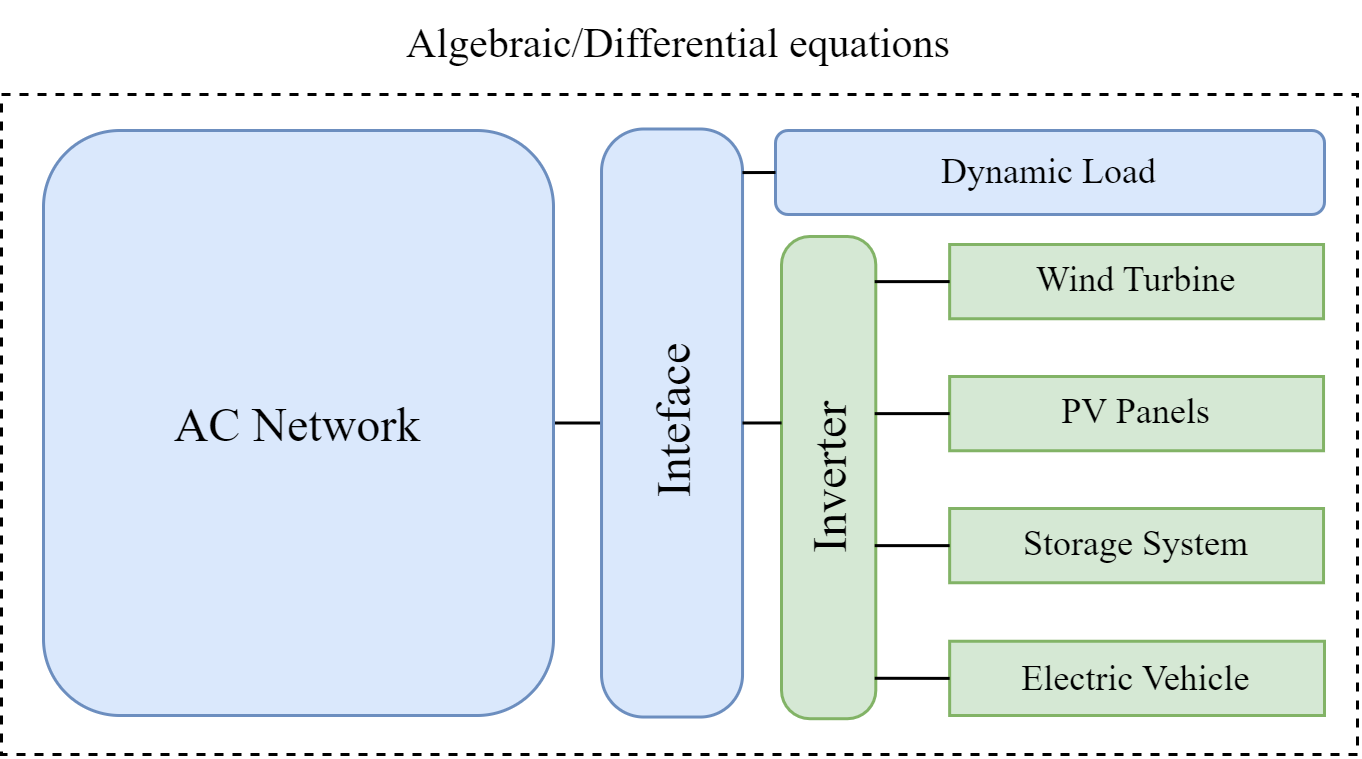
\includegraphics[width = 1\columnwidth]{ps_structure_2.png}
    \caption{Simplified microgrid structure with distributed energy resources.}
    \label{fig:ps_structure}
\end{figure}

\section{Vanadium Redox Flow Battery}\label{sec:ch3/sec1}

A digital twin for vanadium redox flow batteries (VRFBs) offers a powerful framework for real-time, dynamic state monitoring, enabling predictive insights and optimized operation of these large-scale energy storage systems \autocite{10615087}. By creating a high-fidelity virtual replica of the physical battery, the digital twin continuously processes operational data, such as electrolyte flow rates, cell voltages, and temperature profiles, and integrates them with advanced electrochemical models to estimate internal states that are otherwise difficult to measure directly \autocite{Pugach2020, bogdanov_dynamic_2023}. This approach allows operators to detect performance deviations early, forecast SOC and SOH trends, and implement data-driven control strategies to extend battery lifespan and improve efficiency. In this chapter, the DT of VRFB are presented for real-time accurate SOC and output voltage observing.  

To create a digital twin of a VRFB system, it is necessary to consider the the dynamics of main system components that can demonstrate nonlinear behavior at some operating conditions. The good candidate for that is zero dimensional dynamic model that is an  optimal trade off between the complexity and accuracy \autocite{pugach_zero_2018}.

% \subsection{Model Formulation}

In Figure~\cref{fig:vrfb_st}, the traditional configuration of the VRFB system is illustrated.
 \begin{figure}[t]
    \centering
    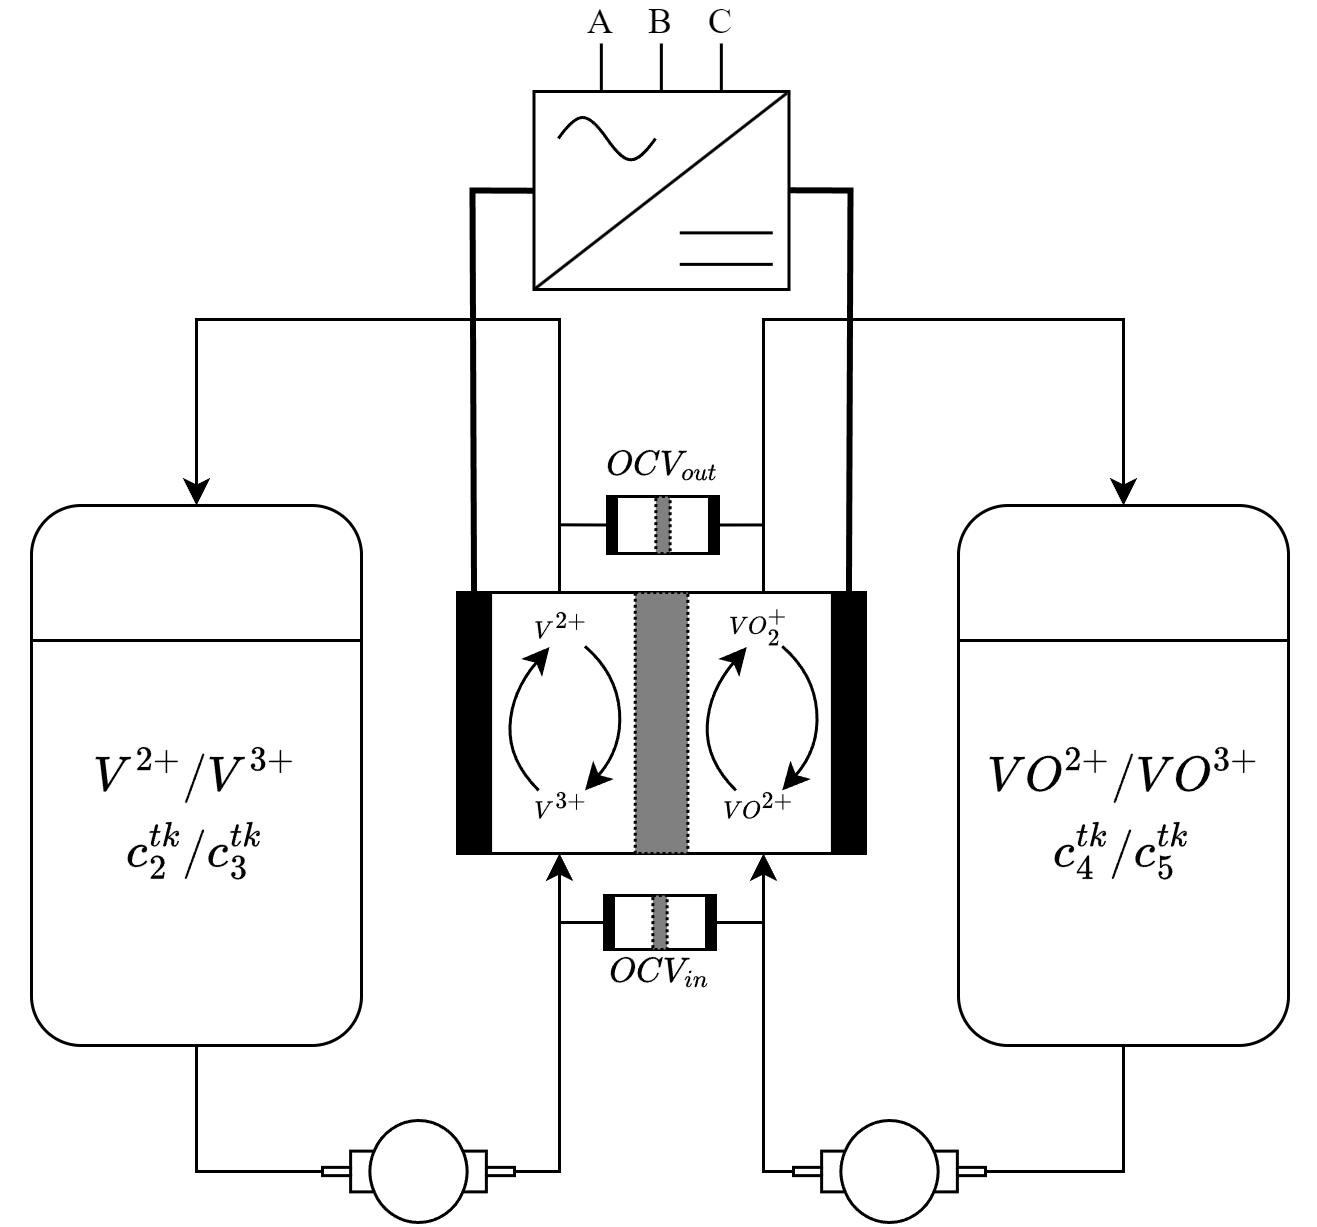
\includegraphics[width = 0.8\columnwidth]{vrfb_diagram.png}
    \caption{A diagram of the VRFB storage system equipped with inlet and outlet open circuit cells.}
    \label{fig:vrfb_st}
    % \vspace*{-0.3cm}
\end{figure}
Vanadium electrolytes contained in two separate tanks with a volume $V_{tk}$ store electrical energy. Via redox reactions electrochemical energy conversions occur in a stack of cells, through which the electrolytes are circulated from the tanks. It's involving the various vanadium $V^{2+}/V^{3+}$ and $V^{4+}/V^{5+}$ redox couples \autocite{ng_understanding_2010}:
\begin{equation}
    \label{eq:redox_pos}
        VO^{2+} + H_2O \rightleftharpoons VO^+_2 + 2H^+ + e^-,
\end{equation}
\begin{equation}
    \label{eq:redox_neg}
        V^{3+} + e^- \rightleftharpoons V^{2+}.
\end{equation}

The configuration of the cell involves a pair of half-cells, divided by a membrane to avoid intermixing. However, transmembrane transfer of certain vanadium ions (crossover) may occur, potentially leading to secondary reactions that contribute to self-discharge and nonlinear voltage fluctuations during both charging and discharging operations.
% \autocite{jrn_pugach_2019}.

The total cell voltage $(U_{cell})$ under a specified load can be resolved into two components: the equilibrium potential and internal losses:
% , as indicated in \autocite{jrn_morozov_2024}:
\begin{equation}
    \label{eq:nernst}
        U_{cell} = U_0^* + \dfrac{RT}{F} \ln{ \left[ \left(\dfrac{c_{5}}{c_{4}}\right)\left(\dfrac{c_{2}}{c_{3}}\right) \right] } + U_{loss},
\end{equation}
where $U_0^*$ is the total cell voltage, $c_2,c_3,c_4,c_5$ are the concentrations of vanadium species $V^{2+}/V^{3+}, VO^{2+},VO_{2}^+$, respectively, $R=\SI{8.314}{J/Kmol}$ is the gas constant, $T=\SI{298}{K}$ is the electrolyte temperature, $F=\SI{96485.332}{C/mol}$ is the Faraday constant. Internal losses are cause the change of cell voltage and offered by activation, ohmic, and concentration overvoltages \autocite{pugach_zero_2018}:

\cref{eq:redox_pos,eq:redox_neg,eq:nernst} clearly show that four different vanadium ions ($V^{2+},V^{3+},V^{4+},V^{5+}$) participate in the battery's redox reactions. Therefore, the instantaneous state of the battery is determined by eight concentrations of vanadium ions, four of which are present within the cell, and the remaining four are situated in the storage tank.

Changes in concentrations within the tank and the cell \autocite{pugach_zero_2018} can be captured by the following equation of the mass balance system in compact matrix form:
% \autocite{jrn_pugach_2022}:
\begin{equation}
    \label{eq:mb_dyn}
        \dot{x} = QAx+ \gamma Jx+Dw,
\end{equation}
where the state vector $x \in \mathbb{R}^{8}$ is represented by eight concentrations of the i-th vanadium ion in the tank and the half-cell:
\begin{equation}
    \label{eq:conc_state}
        x = {\left({c_2^{t},c_3^{t},c_4^{t},c_5^{t},c_2^{cell},c_3^{cell},c_4^{cell},c_5^{cell}}\right)}^T,
\end{equation}

Here, the convection flux due to electrolyte pumping is represented by the flow rate $Q$. The crossover matrix $J$ describes the movement of vanadium ions across the membrane. The system is influenced by an applied current that acts as an external disturbance $w$. To precisely model the effect of the crossover flux, a scaling crossover factor $\gamma$ is applied to modify the overall crossover term.
% \autocite{jrn_bogdanov_2023}.
% Here, the flow rate $Q$ characterizes the convection flux arising from electrolyte pumping. The crossover matrix  $J$ encapsulates vanadium ions fluxes across the membrane. The applied current serves as an external disturbance input to the system $w$. For accurate simulation of crossover flux effect, a scaling crossover factor $\gamma$ is introduced as a multiplicative adjustment to overall crossover term, as it was proposed in our previous work \autocite{jrn_bogdanov_2023}. The matrices are:
\begin{equation}
    \begin{gathered}
    \mathcal{A}=\left[\begin{array}{rr}
    -\alpha & \alpha \\
    \beta & -\beta
    \end{array}\right] \otimes \mathbf{I}_4,
    \end{gathered}
\end{equation}
\begin{equation}
    \begin{gathered}
    \mathcal{J}=\left[\begin{array}{ll}
    0 & 0 \\
    0 & 1
    \end{array}\right] \otimes\left[\begin{array}{rrrr}
    -J_2 & 0 & -J_4 & -2 J_5 \\
    0 & -J_3 & 2 J_4 & 3 J_5 \\
    3 J_2 & 2 J_3 & -J_4 & 0 \\
    -2 J_2 & -J_3 & 0 & -J_5
    \end{array}\right], \\
    \end{gathered}
\end{equation}
\begin{equation}
    \begin{gathered}
    \mathcal{D}=\left[\begin{array}{llllll}
    % 0,0,0,0,{1\over{F V_c}},-{1\over{F V_c}},-{1\over{F V_c}},{1\over{F V_c}}
    0,0,0,0,\frac{1}{F V_c},-\frac{1}{F V_c},-\frac{1}{F V_c},\frac{1}{F V_c}
    \end{array}\right]^{\top}.
    \end{gathered}
\end{equation}

Here, $\mathbf{I}_4 \in \mathbb{R}^{4 \times 4}$ denotes the identity matrix, $\alpha=1 / V_{tk}$, $\beta=1 /\left(n_c V_c\right)$. The Kronecker product is represented as $\otimes$. The matrix $J$ signifies the crossover parasitic dynamics, and its elements  $J_2,J_3,J_4,J_5$, which are functions of the current $w$ \autocite{pugach_zero_2018}.

% The stored energy in the tanks at some moment of time $SOC(t)$ is defined as the ratio of the instantaneous stored energy to the maximum allowable value of the stored energy:
The energy that is stored in the tanks at a particular point in time, $SOC(t)$, is determined by dividing the current stored energy by the highest permissible value of the stored energy \autocite{ng_understanding_2010}:
\begin{equation}
    SOC(t) \equiv E_S(t) / E_{s, \max }.
\end{equation}

The battery's maximum stored energy is directly linked to the cumulative concentration of electrochemical redox pairs. Meanwhile, the energy at any given moment is directly related to the amount of active species present.
% Meanwhile, the instantaneous value of energy is proportional to the concentration of the active species.
% ($V^{2+}$ and $VO^{2+}$ ions). 
Moreover, we should take into account the phenomenon of crossover, which leads to a reduction in SOC. Consequently, the estimation of the SOC is based on the minimum value of the aforementioned ratios \autocite{pugach_zero_2018}:
\begin{equation}
    \label{eq:soc_dt}
    SOC(t)=\min \left(\frac{c_2(t)}{\left(c_2(t)+c_3(t)\right)}, \frac{c_5(t)}{c_5(t)+c_4(t)}\right).
\end{equation}


\subsection{Identification of Parameters}\label{subsec:ch3/sec1/sub1}
The DT application relies on zero-dimensional modeling and real-time measurement data to simulate VRFB behavior. However, during long battery cycling, component degradation leads to parameter mismatch of DT model with battery VRFB system. To maintain accuracy, there is a need to identify parameter values of the battery. 

These are related to internal physical and chemical processes that occur during operation, such as the undesired migration of vanadium ions via the membrane, electrode activation, concentration, and ohmic polarizations, and capacity deterioration over time because of uneven vanadium concentrations. For identification of the VRFB system parameters we used the approach proposed in our previous work \autocite{bogdanov_parameter_2023}.

The VRFB model presented above involves the identification of six unknown parameters, including the equivalent overall vanadium concentration $c_b$, the crossover multiplication factor $\gamma$, the formal potential of the cell $U_0^*$, cell resistivity $r_{c e l l}$, the slope $\alpha$ and the growth rate  $\beta$ of the mass transfer coefficient:
\begin{equation}
    \label{eq:idn}
    \xi=\left(c_b, \gamma, r_{c e l l}, U_0^*, \alpha, \beta\right)^T .
\end{equation}

% The ultimate design of the digital twin for the VRFB state of charge estimator is depicted in Figure~\cref{fig:vrfb_dt}. By leveraging digital twin technology, this state estimator acquires and interprets signals related to current, temperature, and flowrate, achieving real-time monitoring of the battery's state. This setup provides for the exhaustive management and surveillance of the VRFB, capitalizing on the advanced features offered by the digital twin.

In the first step, a discharge polarization curve is experimentally measured at a state of charge $S O C_0$ of $50 \%$ and a specified electrolyte flow rate. Under these conditions, the concentrations of the four vanadium ion species are equal, making the logarithmic term in equilibrium potential is equal to zero. The fitting process involves using an explicit voltage–current relationship:
\begin{equation}
    \label{eq:idt_ubat}
    U_{b a t}(I)=N\left(U_0^*-\frac{|I| \cdot A S R}{\Lambda_{e l}}-\frac{2 R T}{F} \ln \left(1-\frac{|I|}{S O C_0 c_0^* \Lambda_{e l} F u^\beta}\right)\right),
\end{equation}
where $c_0^*=\alpha \cdot c_0$. The parameters are estimated using the least squares method by minimizing the sum of squared differences between the experimental measurements and the simulated values:
\begin{equation}
\begin{aligned}
\min_{c_0^*, ASR, U_0^*, \beta} \quad 
& \varepsilon_1(\xi) = \frac{1}{l} \sum_{m=1}^{l} \left(U^{\text{sim}}_{\text{bat}_m}(\xi, I) - U^{\text{exp}}_{\text{bat}_m}(I)\right)^2 \\
\text{subject to} \quad 
& (c_0^*)^{\min} \leq (c_0^*) \leq (c_0^*)^{\max} \\
& ASR^{\min} \leq ASR \leq ASR^{\max} \\
& (U_0^*)^{\min} \leq (U_0^*) \leq (U_0^*)^{\max} \\
& \beta^{\min} \leq \beta \leq \beta^{\max}
\end{aligned}
\end{equation}
where $l$ represents the total number of points on the polarization curve, and the index $m$ refers to each current data point. Then $c_0^*, \beta, A S R$ and $U_0^*$ are fixed for use in the second stage.

In the second step, the charge-discharge curve is obtained under constant load current and a fixed electrolyte flow rate. The optimization problem is then formulated to minimize the squared error between the measured and simulated voltages during the entire cycle:
\begin{equation}
\begin{aligned}
\min_{c_b, \alpha, \gamma} \quad & \varepsilon(\xi) = \frac{1}{n} \sum_{k=1}^{n} \left(U^{\text{sim}}_{\text{bat}k}(\xi) - U^{\text{exp}}_{\text{bat}k}\right)^2 \\
\text{subject to} \quad & c_b^{\min} \leq c_b \leq c_b^{\max} \\
& \alpha^{\min} \leq \alpha \leq \alpha^{\max} \\
& \gamma^{\min} \leq \gamma \leq \gamma^{\max} \\
& c_b \cdot \alpha = c_b^{*}
\end{aligned}
% \tag{4.11}
\end{equation}
where $n$ denotes the number of data points in a complete charge-discharge cycle, and the index $k$ represents each time step. Parameters $\beta, A S R$ and $U_0^*$ are taken as known from the previous stage.  The nonlinear constraint involving $c_0^*$ to obtain the values of $\alpha$ and $c_0$.  Initial parameter values and allowable ranges $\left[\xi^{\text {min }} ; \xi^{\text {max }}\right]$ are taken from literature data and known properties of the experimental setup. Finally, the optimal set of parameters $\xi$ is obtained and used for simulation under other load conditions.

\section{Power Electronic Interface}\label{sec:ch3/sec2}
The typical configuration of Voltage-Sourced Converter (VSC), shown in Figure~\cref{fig:vsc_scheme}, includes a bidirectional converter with both turn-on and turn-off control capability, optionally a transformer and a condenser on the DC side of the converter \autocite{Milano_2019_ess}. 

\begin{figure}[htbp]
    \centering
    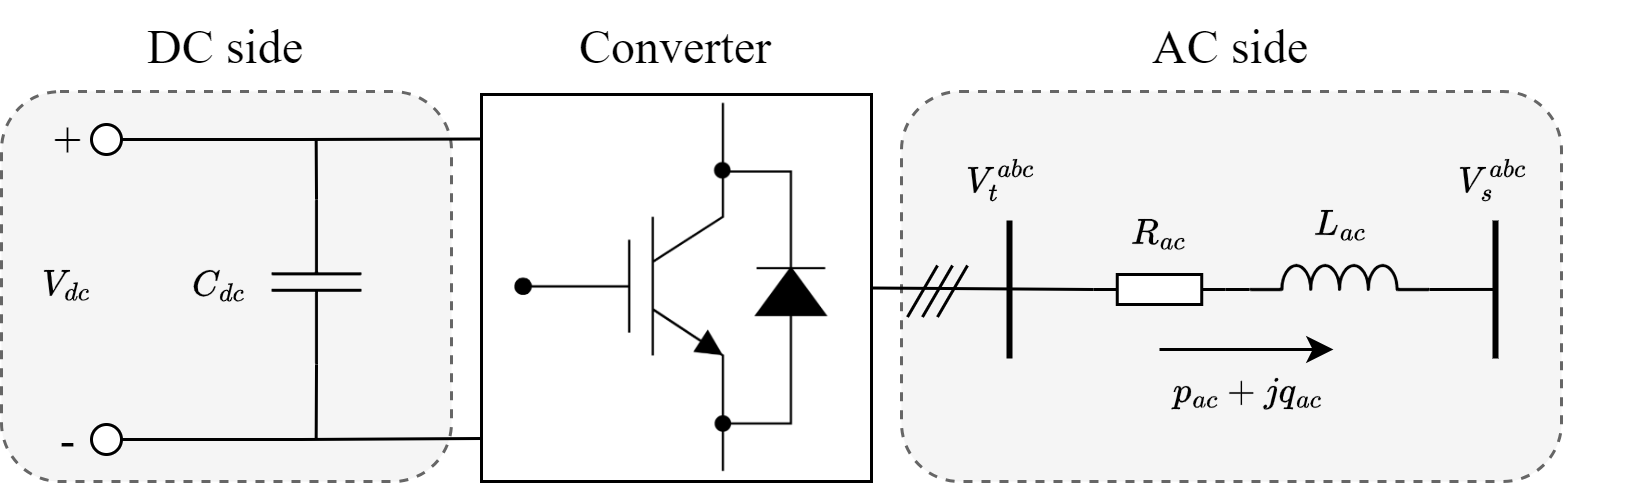
\includegraphics[width = 0.9\columnwidth]{vsc_scheme2.png}
    \caption{Simplified scheme of voltage source converter.}
    \label{fig:vsc_scheme}
\end{figure}

The two-level, three-phase VSC shown in Figure~\cref{fig:2lev_vsc} represents perhaps the most typical configuration among all VSC possibilities. In this setup, each AC terminal is connected to a half-bridge converter, which can assume a voltage of either $v_{\mathrm{dc}} / 2$ or $-v_{\mathrm{dc}} / 2$, where $v_{\mathrm{dc}}$ denotes the DC-side voltage of the converter. Each half-bridge converter consists of two fully controllable reverse-conducting switch cells, each made up of a transistor $\mathrm{T}_i$ and an antiparallel diode $\mathrm{D}_i$ (where $i=1,2,\ldots,6$). Typical examples of such switches include the integrated gate bipolar transistor and the integrated gate-commutated thyristor.

\begin{figure}[htbp]
    \centering
    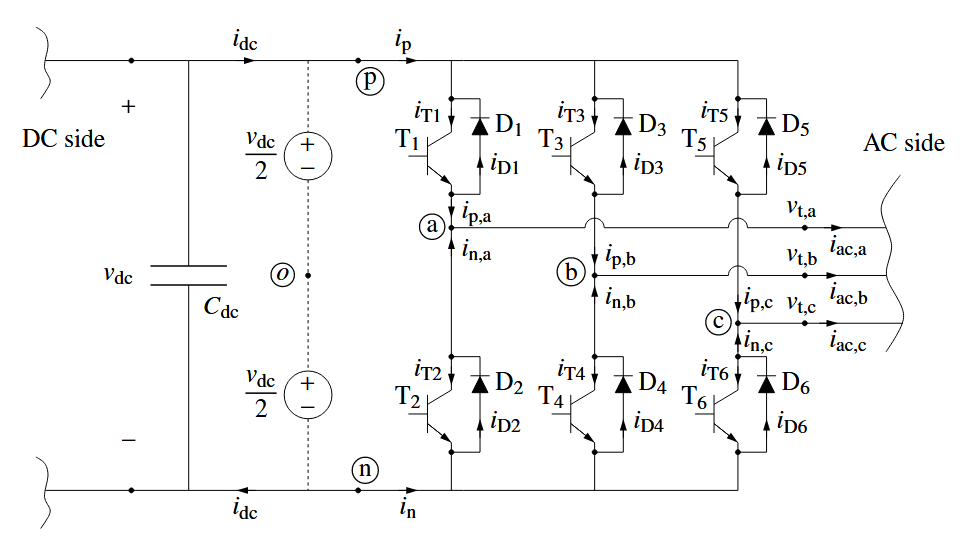
\includegraphics[width = 0.85\columnwidth]{2lev_vsc.png}
    \caption{Ideal two-level three-phase VSC diagram.}
    \label{fig:2lev_vsc}
\end{figure}

The voltage, $v_{\mathrm{t, abc}}$, on the AC side of the converter is influenced by both $v_{\mathrm{dc}}$ and the switching logic characteristic of $\mathrm{T}_i$, derived via PWM control \autocite{mohan2003power}. PWM works by comparing a high-frequency carrier signal ( $f_{\text {carr }} \sim \mathrm{kHz}$ ), typically of triangular shape ( $[-1,1]$ ), with a lower-frequency modulation signal. In two-level, three-phase VSCs, this modulation signal comprises three-phase balanced sinusoidal functions, meaning $\boldsymbol{v}_{\mathrm{t, abc}}$ has equal amplitudes across its three phases, each separated by a $2 \pi / 3$ rad phase shift \autocite{Milano_2019_ess}.

The switching logic of $\mathrm{T}_1, \mathrm{~T}_3$ and $\mathrm{T}_5$ is as follows:
\begin{equation}
    \begin{aligned}
    k_{\mathrm{T} 1,3,5}(t)= \begin{cases}1, & \text { if the modulating signal exceeds the carrier signal, } \\ 0, & \text { otherwise }\end{cases}
    \end{aligned}
\end{equation}

The states of $\mathrm{T}_2, \mathrm{~T}_4$, and $\mathrm{T}_6$ are inverse to those of $\mathrm{T}_1, \mathrm{~T}_3$, and $\mathrm{T}_5$. Hence,
\begin{equation}
    \begin{aligned}
    k_{\mathrm{T} 1}(t)+k_{\mathrm{T} 2}(t)=k_{\mathrm{T} 3}(t)+k_{\mathrm{T} 4}(t)=k_{\mathrm{T} 5}(t)+k_{\mathrm{T} 6}(t)=1.
    \end{aligned}
\end{equation}

The switch is closed when $k_{\mathrm{T} i}=1$, allowing the AC current $\boldsymbol{i}_{\mathrm{ac}, \mathrm{abc}}$ to flow in required direction.

The switching model can accurately represent the behavior of the ideal VSC. More detailed models of the switches that take into account switching losses, snubber circuits, etc., can be used for an accurate representation of the converter dynamic behavior. Such detailed models show some drawbacks, as follows \autocite{Milano_2019_ess}:
\begin{itemize}
    \item Modeling the dynamics of circuitry and controllers in a switching framework is often challenging. 
    \item In models with large time scales relative to converter switching, high-frequency circuit dynamics are typically ignored.
    \item Transient stability studies with switching models are computationally heavy due to the need for microsecond time steps. 
\end{itemize}

The converter's averaged model addresses these challenges \autocite{sira2006control,middlebrook1976ieee}, by averaging the converter's instantaneous values over a time period typically corresponding to the carrier signal's switching period. In this model, the terminal voltage at the AC side of the VSC can be expressed as a function of the modulating signal, as follows:
\begin{equation}
    \begin{aligned}
        \underline{v}_{\mathrm{t}}^{abc}(t)=\frac{v_{\mathrm{dc}}}{2} \boldsymbol{m}_{\mathrm{abc}}(t)=\frac{v_{\mathrm{dc}}}{2}\left[\begin{array}{l}
        m(t) \cos \left(\omega_{\mathrm{ms}}(t) t+\theta_o\right) \\
        m(t) \cos \left(\omega_{\mathrm{ms}}(t) t+\theta_o-\frac{2 \pi}{3}\right) \\
        m(t) \cos \left(\omega_{\mathrm{ms}}(t) t+\theta_o+\frac{2 \pi}{3}\right)
        \end{array}\right]
    \end{aligned}
\end{equation}
where $m$ denotes the amplitude, $\omega_{\mathrm{ms}}$ represents the frequency of the modulating signal, and $\theta_o$ is the phase offset.

\subsection{Coordinate Transformation}

During the modeling process, three coordinate systems are interrelated to describe dynamic states within the network and control loop: the three-phase, $\alpha \beta$, and $dq$ coordinates. Figure~\cref{fig:coord_transform} illustrates the transformation between these. The Clarke transformation \autocite{6739414} converts the three-phase sinusoidal variables into rotated real and imaginary components. Variables in the $\alpha \beta$-coordinate are expressed as follows:
\begin{equation}
    \begin{aligned}
        \underline{x}(t)=x_a(t)+j \cdot x_\beta(t)
    \end{aligned}
\end{equation}
where $x_\alpha$ and $x_\beta$ denote the real and imaginary components of the state variable $\underline{x}(t)$. The transformation from three-phase to $\alpha \beta$ coordinates employs the general matrix $T_{\mathrm{M}}$.

\begin{equation}
    \begin{aligned}
        \left[\begin{array}{l}
        x_0 \\
        x_{\alpha} \\
        x_{\beta}
        \end{array}\right]=T_{\mathrm{M}} \cdot\left[\begin{array}{l}
        x_{\mathrm{a}} \\
        x_{\mathrm{b}} \\
        x_{\mathrm{c}}
        \end{array}\right]=\frac{1}{3} \cdot\left[\begin{array}{ccc}
        1 & 1 & 1 \\
        2 & -1 & -1 \\
        0 & \sqrt{3} & -\sqrt{3}
        \end{array}\right] \cdot\left[\begin{array}{l}
        x_{\mathrm{a}} \\
        x_{\mathrm{b}} \\
        x_{\mathrm{c}}
        \end{array}\right]
    \end{aligned}
\end{equation}
where the variables $x_\alpha$ and $x_\beta$ are given by
\begin{equation}
    \begin{aligned}
        & x_{\mathrm{a}}=\frac{1}{3}\left(2 \cdot x_{\mathrm{a}}-x_{\mathrm{b}}-x_{\mathrm{c}}\right) \\
        & x_\beta=\frac{1}{3}\left(\sqrt{3} \cdot x_{\mathrm{b}}+\sqrt{3} \cdot x_{\mathrm{c}}\right)
    \end{aligned}
\end{equation}
In a three-phase system, the states $x_{\mathrm{a}}, x_{\mathrm{b}}, x_{\mathrm{c}}$ transform into two main components due to system symmetry, simplifying representation through space vector for both instantaneous and amplitude values. This results in a fully decoupled system. For controller design, converting from stationary three-phase and $\alpha \beta$ coordinates to a rotating system with rotor speed is practical. This system, aligned with the rotor or pole wheel (see Figure~\cref{fig:coord_transform}), benefits from easier representation of electrical dynamics and transforms sinusoidal variables into steady-state form, enabling classical control strategies similar to the well-controlled DC machine. The $\alpha \beta$ to $dq$-coordinate transformation is denoted by

\begin{equation}
    \begin{aligned}
        \left[\begin{array}{l}
        x_{\mathrm{d}} \\
        x_{\mathrm{q}}
        \end{array}\right]=T_{\mathrm{R}} \cdot\left[\begin{array}{l}
        x_\alpha \\
        x_\beta
        \end{array}\right]=\left[\begin{array}{cc}
        \cos \varphi & \sin \varphi \\
        -\sin \varphi & \cos \varphi
        \end{array}\right] \cdot\left[\begin{array}{l}
        x_\alpha \\
        x_\beta
        \end{array}\right]
    \end{aligned}
\end{equation}

where $\varphi=\omega t$ is the angle of the difference between both coordinates. $T_{\mathrm{R}}$ is the transformation matrix for $dq$-coordinate.

\begin{figure}[htbp]
    \centering
    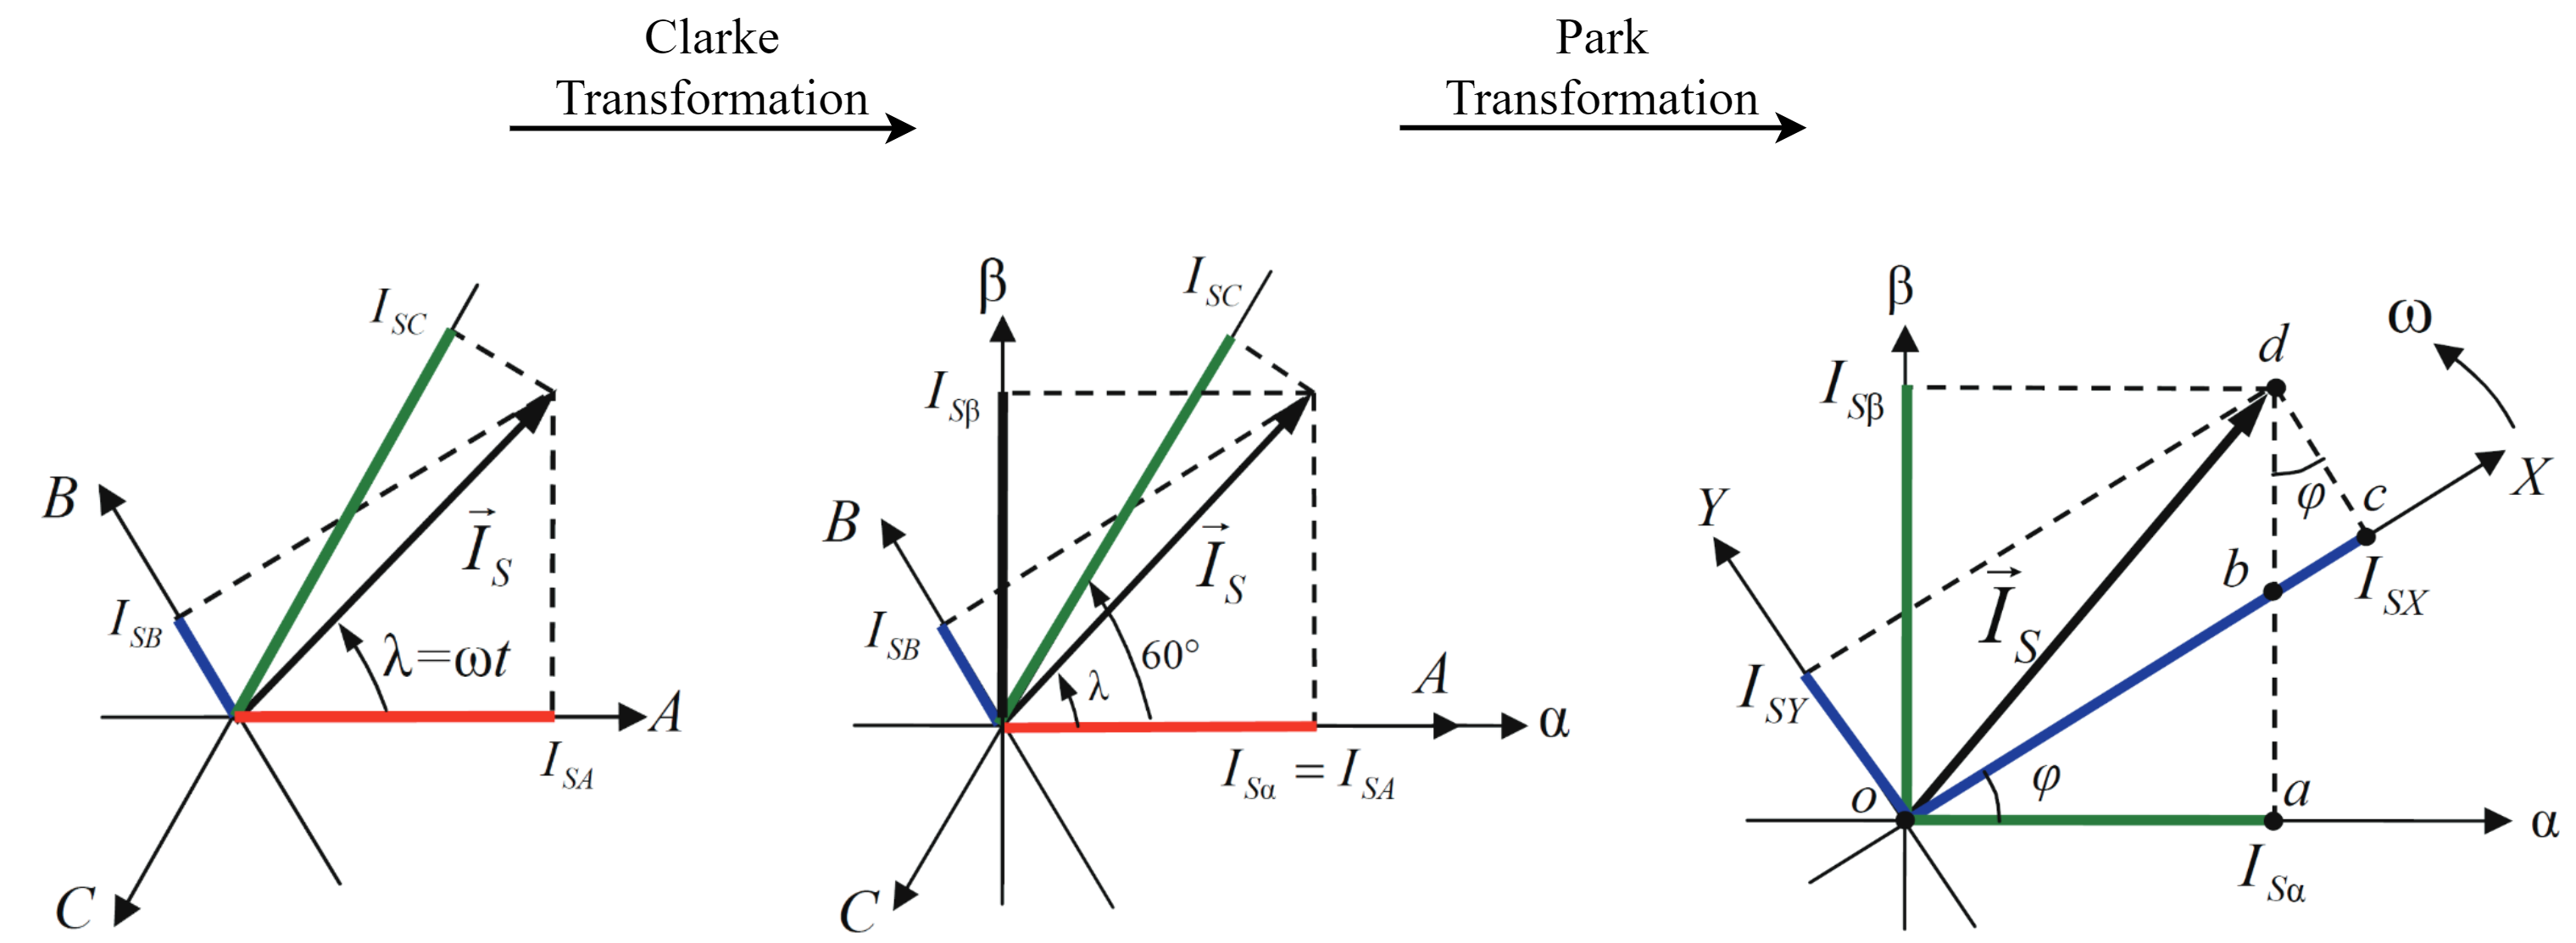
\includegraphics[width = \columnwidth]{coord_transform.png}
    \caption{Transformation of three-phase coordinate, $\alpha \beta$-coordinate, and $dq$-coordinate \autocite{Kalachev2013}.}
    \label{fig:coord_transform}
\end{figure}

Unlike the $\alpha \beta$-frame control, $dq$-frame control necessitates a synchronization method, typically provided by the phase-locked loop (PLL), which is considered a drawback of the $dq$-frame control.

\subsection{Dynamic Model of Power Controller}\label{subsec:ch3/sec2/sub2}
To observe dynamics of the power system, the real-/reactive-power controller in $dq$-frame will be analyzed.
% To observe dynamics of the power system, the simplified diagram in Figure~\cref{fig:grid_following} of a current-controlled real-/reactive-power controller in $dq$-frame will be analyzed.

% \begin{figure}[htbp]
%     \centering
%     \includegraphics[width = \columnwidth]{graphics/grid_following.png}
%     \caption{Schematic diagram of a current-controlled real-/reactive-power controller in dq-frame.}
%     \label{fig:grid_following}
% \end{figure}

The AC system voltage in the VSC system can be expressed as
\begin{equation}
    \begin{array}{l}
        V_{s a}(t)=\widehat{V}_{s} \cos \left(\omega_{0} t+\theta_{0}\right) \\
        V_{s b}(t)=\widehat{V}_{s} \cos \left(\omega_{0} t+\theta_{0}-\frac{2 \pi}{3}\right), \\
        V_{s c}(t)=\widehat{V}_{s} \cos \left(\omega_{0} t+\theta_{0}-\frac{4 \pi}{3}\right),
    \end{array}
\end{equation}
where $\widehat{V}_s$ is the peak value of the line-to-neutral voltage, $\omega_0$ is the frequency of the AC system, and $\theta_0$ is the angle of initial phase of the source. The space phasor equivalent of $V_{s-a b c}$ is
\begin{equation}
    \begin{aligned}
        \label{eq:v_phasor}
        \vec{V}_s(t)=\widehat{V}_s e^{j\left(\omega_0 t+\theta_0\right)}.
    \end{aligned}
\end{equation}

Dynamics of the AC side of the system are described by the following space-phasor equation:
\begin{equation}
    \label{eq:inv_dynamic}
    \begin{aligned}
        L \frac{d \vec{i}}{d t}=-R \vec{i}+\vec{V}_t-\vec{V}_s.
    \end{aligned}
\end{equation}

This can be decomposed into real and imaginary components:
\begin{equation}
    \label{eq:inv_nonlinear}
    \begin{aligned}
        & L \frac{d i_d}{d t}=L \omega(t) i_q-R i_d+V_{t d}-\widehat{V}_s \cos \left(\omega_0 t+\theta_0-\rho\right), \\
        & L \frac{d i_q}{d t}=-L \omega(t) i_d-R i_q+V_{t q}-\widehat{V}_s \sin \left(\omega_0 t+\theta_0-\rho\right), \\
        & \frac{d \rho}{d t}=\omega(t).
    \end{aligned}
\end{equation}

The further investigation will lead to:
\begin{equation}
    \begin{aligned}
        & L \frac{d i_d}{d t}=L \omega_0 i_q-R i_d+V_{t d}-\widehat{V}_s, \\
        & L \frac{d i_q}{d t}=-L \omega_0 i_d-R i_q+V_{t q}.
    \end{aligned}
\end{equation}
which describe a second-order linear system influenced by the steady input $\widehat{V}_s$. Therefore, with $V_{t d}$ and $V_{t q}$ as DC values, $i_d$ and $i_q$ also remain DC in the steady state. The method that ensures $\rho(t)=\omega_0 t+\theta_0$ is the PLL \autocite{book_yazdani_2010}. The next section outlines the PLL's structure, modeling, and stabilization.

\subsection{Grid Synchronization}\label{subsec:ch3/sec2/sub3}
PLL ensures the $dq$ frame aligns with the grid voltage phasor's rotation \autocite{cole2010vsc, 5637778}. Figure~\cref{fig:pll_basic} illustrates the fundamental-frequency model of a PLL. 

\begin{figure}[htbp]
    \centering
    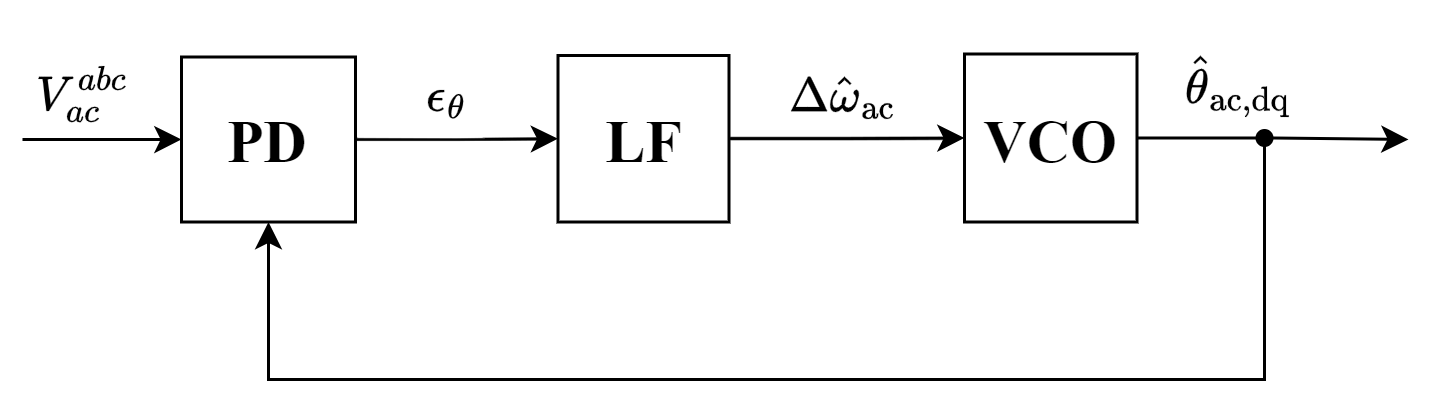
\includegraphics[width = 0.8\columnwidth]{pll_basic.png}
    \caption{Basic scheme of a PLL \autocite{Milano_2019_ess}.}
    \label{fig:pll_basic}
\end{figure}
Key components include \autocite{Milano_2019_ess}:
\begin{itemize}
    \item The Phase Detector (PD) evaluates the three-phase voltage vector, $V_{ac}^{abc}$, at the connection bus and computes the phase angle offset, $\epsilon_\theta$, between the measured phase angle, $\hat{\theta}_\mathrm{ac}$, and the $dq$ frame angle estimated by the PLL, $\hat{\theta}_{\mathrm{ac}, \mathrm{dq}}$. The voltage first transitions from ‘$abc$’ to ‘$\alpha\beta\gamma$’, and subsequently to ‘$dqo$’ components.
     \item The Loop Filter (LF) processes the error $\epsilon_\theta$ between actual and estimated voltage phase angles. Despite various LF configurations, they are typically designed as perfect tracking controllers that ensure $\epsilon_\theta = 0$ in steady state. Notably, the LF output estimates the frequency deviation at the connection bus, $\Delta \hat{\omega}_{\mathrm{ac}}$.
     \item The Voltage Controlled Oscillator (VCO) uses the bus frequency shift $\Delta \hat{\omega}_{\mathrm{ac}}$ to estimate the $dq$-frame phase angle $\hat{\theta}_{\mathrm{ac}, \mathrm{dq}}$, generally operating with an integrator that stabilizes to $\Delta \hat{\omega}_{\mathrm{ac}}$.
\end{itemize}

More detailed control diagram is presented in Figure~\cref{fig:pll_control}, forming a dynamic equation: 
\begin{equation}
     \frac{d\rho}{dt} = \hat{V}_{s} H(p) (\omega_{0} t + \theta_{0} - \rho),
\end{equation}
\noindent which represents a feedback control loop in which $\omega_{0} t + \theta_{0}$ is the reference input, $\rho$ is obtained angle, and $H(s)$ is the compensator transfer function. The dynamic performance of the PLL is greatly affected by the compensator H(s). In real conditions, the compensator should be able to deal with unbalanced and/or harmonically distorted three-phase voltages. In this work, we assume the ideal balanced voltage conditions and apply PLL compensator as PI controller only.

\begin{figure}[htbp]
    \centering
    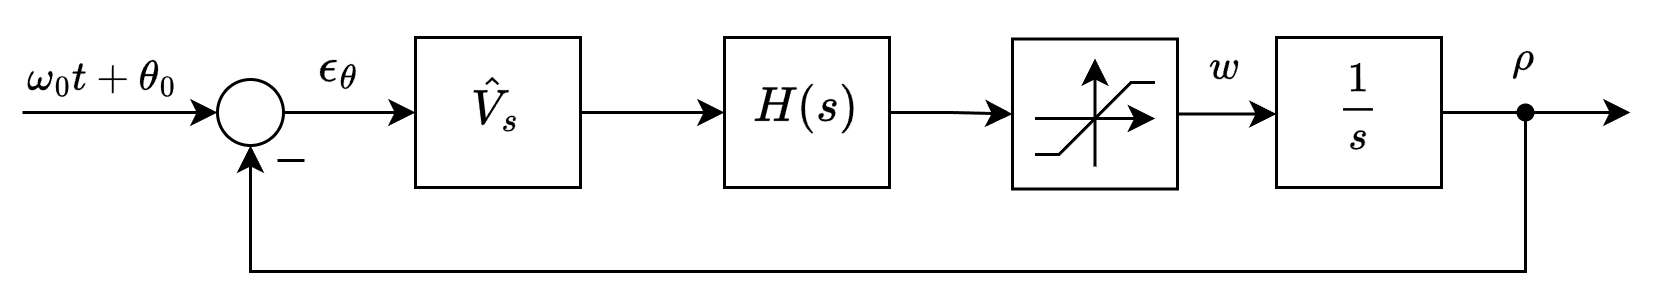
\includegraphics[width = \columnwidth]{pll_control.png}
    \caption{Basic inverter control block diagram of PLL \autocite{6739414}}
    \label{fig:pll_control}
\end{figure}

\subsection{Control}\label{subsec:ch3/sec2/sub4}
Suggesting ideal angle matching within PLL and applying Park transformation the expression of the terminal voltage of the AC side of the converter, $V_{t}^{abc}$, can be written in the $dq$ frame as follows:
\begin{equation}
    v_{\mathrm{t}, \mathrm{dq}}(t)=\left[\begin{array}{c}
v_{\mathrm{t}, \mathrm{~d}}(t) \\
v_{\mathrm{t}, \mathrm{q}}(t)
\end{array}\right]=\mathbf{P} \frac{v_{\mathrm{dc}}}{2}\left[\begin{array}{c}
m_{\mathrm{a}}(t) \\
m_{\mathrm{b}}(t) \\
m_{\mathrm{c}}(t)
\end{array}\right]=\frac{v_{\mathrm{dc}}}{2}\left[\begin{array}{c}
m_{\mathrm{d}}(t) \\
m_{\mathrm{q}}(t)
\end{array}\right],
\label{eq:v_dq_transf}
\end{equation}
where $\mathbf{P}$ is the Park tensor, the system under balanced conditions and the nominal frequency.

The expression of the complex power of the AC side of the VSC, $\bar{s}_{\mathrm{ac}}$, projected onto the $dq$ frame is:
\begin{equation}
    \begin{aligned}
        \bar{s}_{\text{ac}}(t) &= p_{\text{ac}}(t) + j q_{\text{ac}}(t) = \frac{3}{2} \left( \bar{v}_{\text{ac,dq}}(t) \bar{i}_{\text{ac,dq}}^*(t) \right) \\
        &= \frac{3}{2} \left[ v_{\text{ac,d}}(t) i_{\text{ac,d}}(t) + v_{\text{ac,q}}(t) i_{\text{ac,q}}(t) \right. \\
        &\quad \left. +\, j \left( v_{\text{ac,q}}(t) i_{\text{ac,d}}(t) - v_{\text{ac,d}}(t) i_{\text{ac,q}}(t) \right) \right],
    \end{aligned}
\end{equation}

Thus:
\begin{equation}
    \begin{aligned}
        \begin{array}{l}
            p_{\mathrm{ac}}(t)=\operatorname{Re}\left\{\bar{s}_{\mathrm{ac}}(t)\right\}=\displaystyle\frac{3}{2}\left(v_{\mathrm{ac}, \mathrm{~d}}(t) i_{\mathrm{ac}, \mathrm{~d}}(t)+v_{\mathrm{ac}, \mathrm{q}}(t) i_{\mathrm{ac}, \mathrm{q}}(t)\right) \\[1em]
            q_{\mathrm{ac}}(t)=\operatorname{Im}\left\{\bar{s}_{\mathrm{ac}}(t)\right\}=\displaystyle\frac{3}{2}\left(v_{\mathrm{ac}, \mathrm{q}}(t) i_{\mathrm{ac}, \mathrm{~d}}(t)-v_{\mathrm{ac}, \mathrm{~d}}(t) i_{\mathrm{ac}, \mathrm{q}}(t)\right) .
        \end{array}
    \end{aligned}
\end{equation}
where $v_{ac,d}$ and $v_{ac,q}$ are the $dq$-frame voltage components of the AC system and cannot be controlled by the VSC system. If the PLL is in a steady state, $v_{ac,q}=0$ and can be rewritten as

\begin{equation}
    \begin{aligned}
        \begin{array}{l}
            p_{\mathrm{ac}}(t) = \displaystyle\frac{3}{2} v_{\mathrm{ac}, \mathrm{~d}}(t)i_{\mathrm{ac}, \mathrm{~d}}(t), \\[1em]
            q_{\mathrm{ac}}(t) = -\displaystyle\frac{3}{2} V_{sd}(t)i_q(t).
        \end{array}
    \end{aligned}
\end{equation}

Based on that, $p_{\mathrm{ac}}(t)$ and $q_{\mathrm{ac}}(t)$ can be controlled by $id$ and $iq$, respectively.

\begin{equation}
    \begin{aligned}
        i_{dref}(t) & =\frac{2}{3V_{sd}} P_{sref}(t) \\[1em]
        i_{qref}(t) & =-\frac{2}{3 V_{sd}} Q_{sref}(t)
    \end{aligned}
\end{equation}

\textbf{Grid-Following Mode}. In most cases, where an inverter is involved in delivering power from DER or ESS to the grid, it works in grid following mode, where real (DC) and reactive (AC) powers (voltages) are regulated by means of the components of the current $i_{ac}^{abc}$ \autocite{720325}. 
The control scheme consists of current control loop and reference signal generator. It allows us to protect the VSC against possible overcurrents. Moreover, current-mode control includes dynamic performance, overload rejection, and robustness against changes in load parameters.

The scheme of the inner current control loop of the VSC coupled to the converter is shown in Figure~\cref{fig:inv_cc}.

\begin{figure}[htbp]
    \centering
    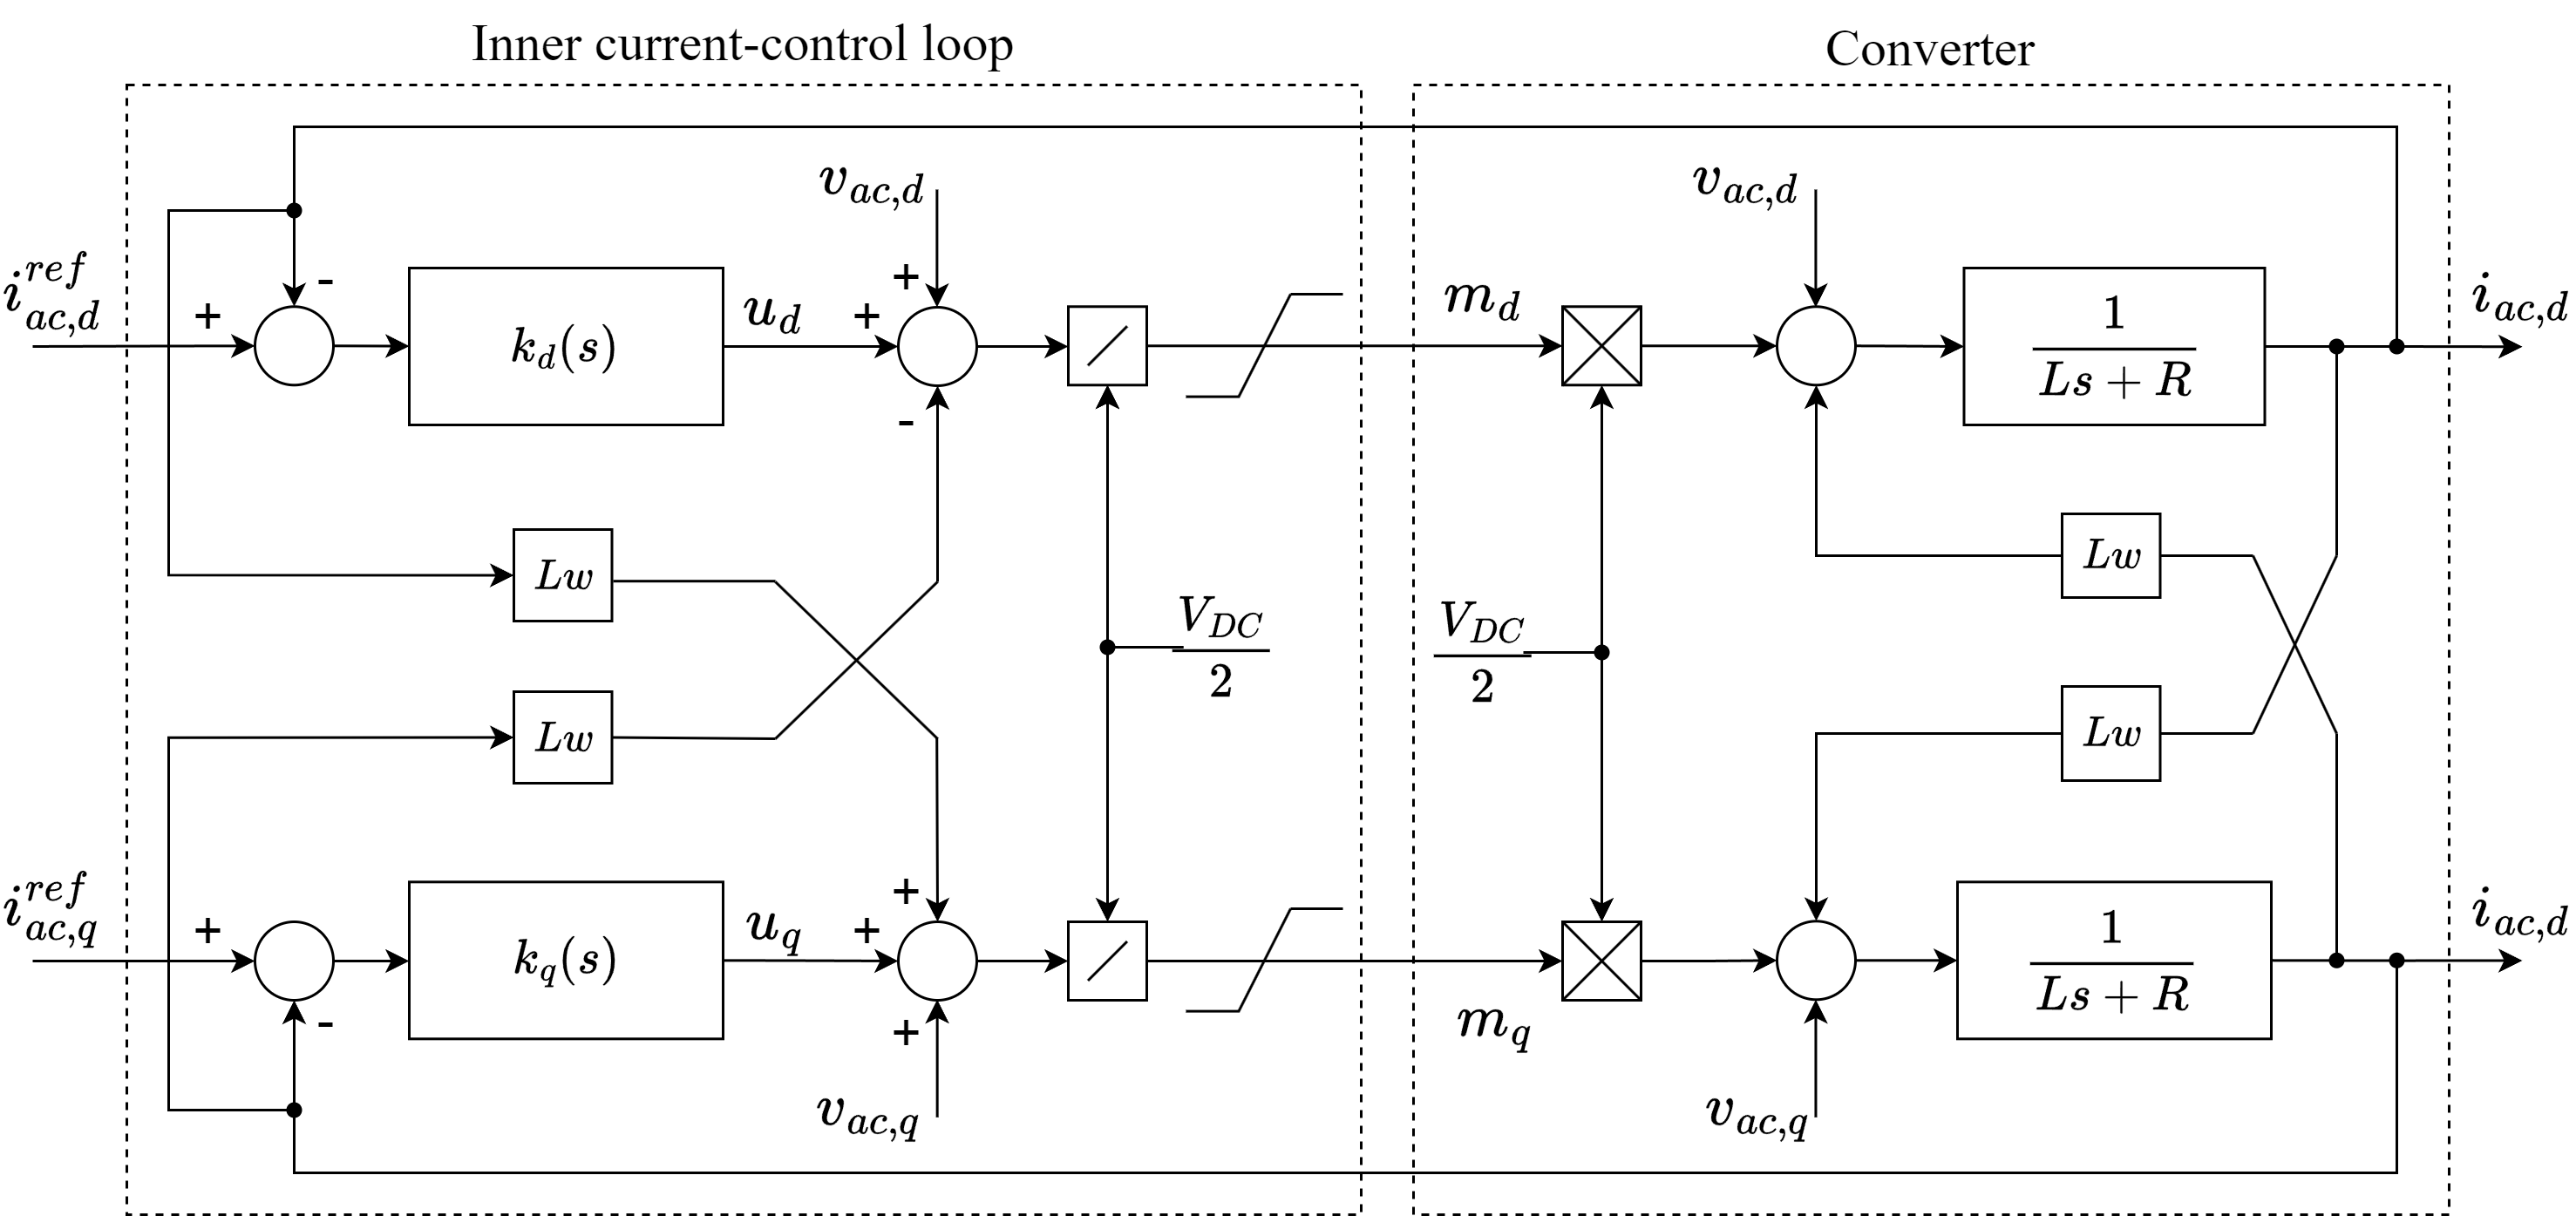
\includegraphics[width = 1\columnwidth]{inv_cc.png}
    \caption{VSC grid-following control diagram in the dq frame}
    \label{fig:inv_diagram_gfl}
\end{figure}

The $dq$-frame control of the active/reactive-current controller here is based on \ref{eq:inv_nonlinear}. Assuming a steady-state and setting $\omega(t)$ to $\omega_0$, we conclude
\begin{equation}
    \begin{array}{l}
L \displaystyle\frac{d i_{d}}{d t}=L \omega_{0} i_{q}-R i_{d}+V_{t d}-V_{s d} \\[1em]
L \displaystyle\frac{d i_{q}}{d t}=-L \omega_{0} i_{d}-R i_{q}+V_{t q}-V_{s q}
\end{array}
\end{equation}

As can be seen, $L\omega_0$ terms bring coupling to the $id$ and $iq$ dynamics. Applying $dq$ transformation \ref{eq:v_dq_transf} we can determine $m_d$ and $m_q$ to decouple the dynamics as 
\begin{equation}
    \begin{aligned}
m_{d} & =\frac{2}{V_{D C}}\left(u_{d}-L \omega_{0} i_{q}+V_{s d}\right) \\
m_{q} & =\frac{2}{V_{D C}}\left(u_{q}+L \omega_{0} i_{d}+V_{s q}\right)
\end{aligned}
\end{equation}
where $u_d$ and $u_q$ are two control inputs, which are the outputs of two corresponding compensators, shown in Figure~\cref{fig:inv_cc_pi}. Basically, $k_d(s)$ can be a simple proportional-integral (PI) compensator to track the DC reference signal.

\begin{figure}[htbp]
    \centering
    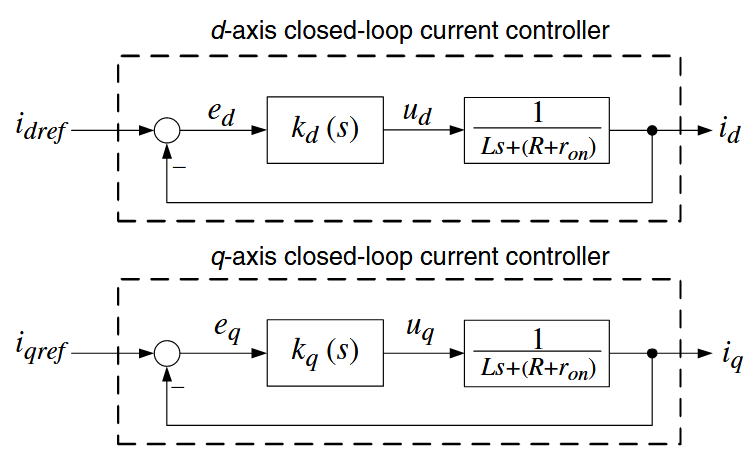
\includegraphics[width = 0.7\columnwidth]{inv_cc_pi.png}
    \caption{Simplified block diagram of the current-controlled VSC \autocite{book_yazdani_2010}.}
    \label{fig:inv_cc_pi}
\end{figure}

Let us assume PI regulator
\begin{equation}
    k_{d}(s)=\frac{k_{p} s+k_{i}}{s},
\end{equation}
where $k_p$ denotes the proportional gain and $k_i$ represents the integral gain. 

It can be seen from Figure~\cref{fig:inv_cc_pi}, that the transfer function of the closed-loop system can be reduced to first order
\begin{equation}
    \frac{I_{d}(s)}{I_{d r e f}(s)}=G_{i}(s)=\frac{1}{\tau_{i} s+1},
\end{equation}
in case of
\begin{equation}
    \begin{array}{l}
k_{p}=L / \tau_{i}, \\
k_{i}=\left(R+r_{o n}\right) / \tau_{i}.
\end{array}
\label{eq:cc_pi}
\end{equation}
where $\tau_i$ is the time constant of the resultant closed-loop system. The final view of the averaged model of inverter with control blocks in grid-following mode will take the form:
\begin{figure}[htbp]
    \centering
    \includegraphics[width = 1\columnwidth]{grid_following.png}
    \caption{Simplified block diagram of the VSC in grid-following mode}
    \label{fig:inv_cc}
\end{figure}

\textbf{Grid-Forming Mode}. In case of system transit to island mode without an external grid, an inverter switches to grid-forming mode. In this mode, the goal is to maintain the load voltage's amplitude and frequency despite fluctuations in load current. To prevent switching current harmonics penetrate into the load, $C_f$ appears to $RL$ filter. The control here can be realized here in $dq$-frame as in grid-following mode, while the angle for transformations, $\rho$, is obtained from the output of a VCO whose input is $d\rho/dt = \omega(t)$. $\omega(t)$ can be set as nominal frequency of the power system, $\omega_0$, or it can be dynamically controlled in a variable-frequency environment \autocite{5275592}. The averaged model of inverter with control blocks in grid-forming mode has the form:
\begin{figure}[htbp]
    \centering
    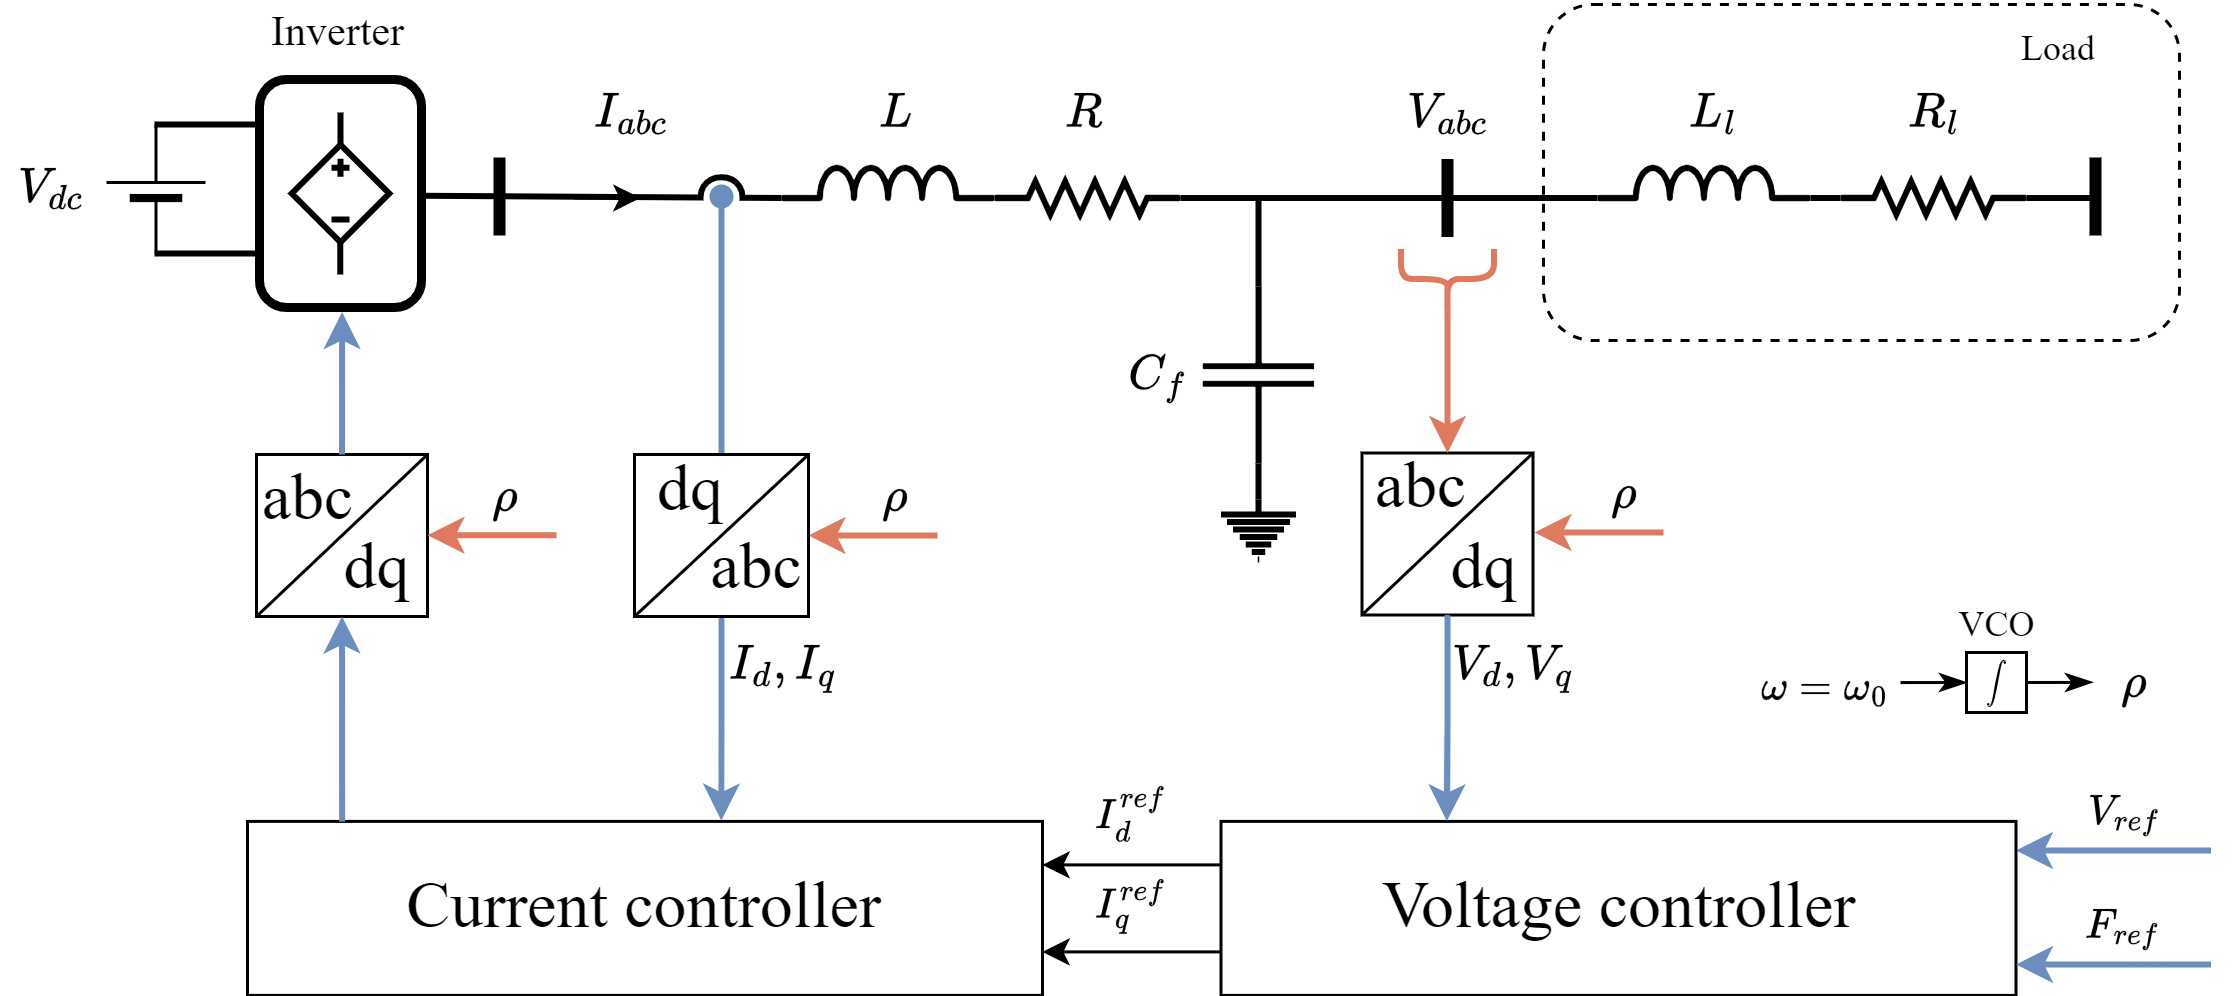
\includegraphics[width = 0.95\columnwidth]{grid_forming.png}
    \caption{Simplified block diagram of the VSC in grid-forming mode}
    \label{fig:inv_gf}
\end{figure}

The voltage, delivered to the load in this case will take the form in terms of its $dq$-frame components:
\begin{equation}
    \begin{aligned}
        C_{f} \frac{d V_{s d}}{d t} & =C_{f}\left(\omega V_{s q}\right)+i_{d}-i_{L d} \\
        C_{f} \frac{d V_{s q}}{d t} & =-C_{f}\left(\omega V_{s d}\right)+i_{q}-i_{L q},
    \end{aligned}
    \label{eq:inv_vc}
\end{equation}
where $d\rho/dt$ has been replaced by $\omega(t)$. 

Equations \ref{eq:inv_vc} illustrate the dynamics of $V_{sd}$ and $V_{sq}$. Here, $V_{sd}$ and $V_{sq}$ represent system outputs, while $i_d$, $i_q$, and $\omega$ act as control inputs. Furthermore, $i_d$ and $i_q$ respond to the d- and q-axis current controllers of the VSC system, based on $i_{dref}$ and $i_{qref}$, respectively.

As shown in Figure~\cref{fig:inv_vc}, $V_{sd}$ and $V_{sq}$ can be controlled by $i_{dref}$ and $i_{qref}$, while also being interconnected, reflecting the effects of $i_{Ld}$ and $i_{Lq}$. This relation is determined as follows
\begin{equation}
    \begin{array}{l}
        i_{d r e f}=u_{d}-C_{f}\left(\omega V_{s q}\right)+i_{L d}, \\
        i_{q r e f}=u_{q}+C_{f}\left(\omega V_{s d}\right)+i_{L q} .
    \end{array}
\end{equation}
where $u_d$ and $u_q$ are two new control inputs, which are the outputs of two independent compensators. It can be seen that decoupling feed-forward compensation are required, which is similar to the one utilized to decouple $i_d$ and $i_q$ in a current-controlled VSC. The final view of the control diagram in the $dq$ frame is shown in Figure~\cref{fig:inv_diagram_gfm}.

\begin{figure}[htbp]
    \centering
    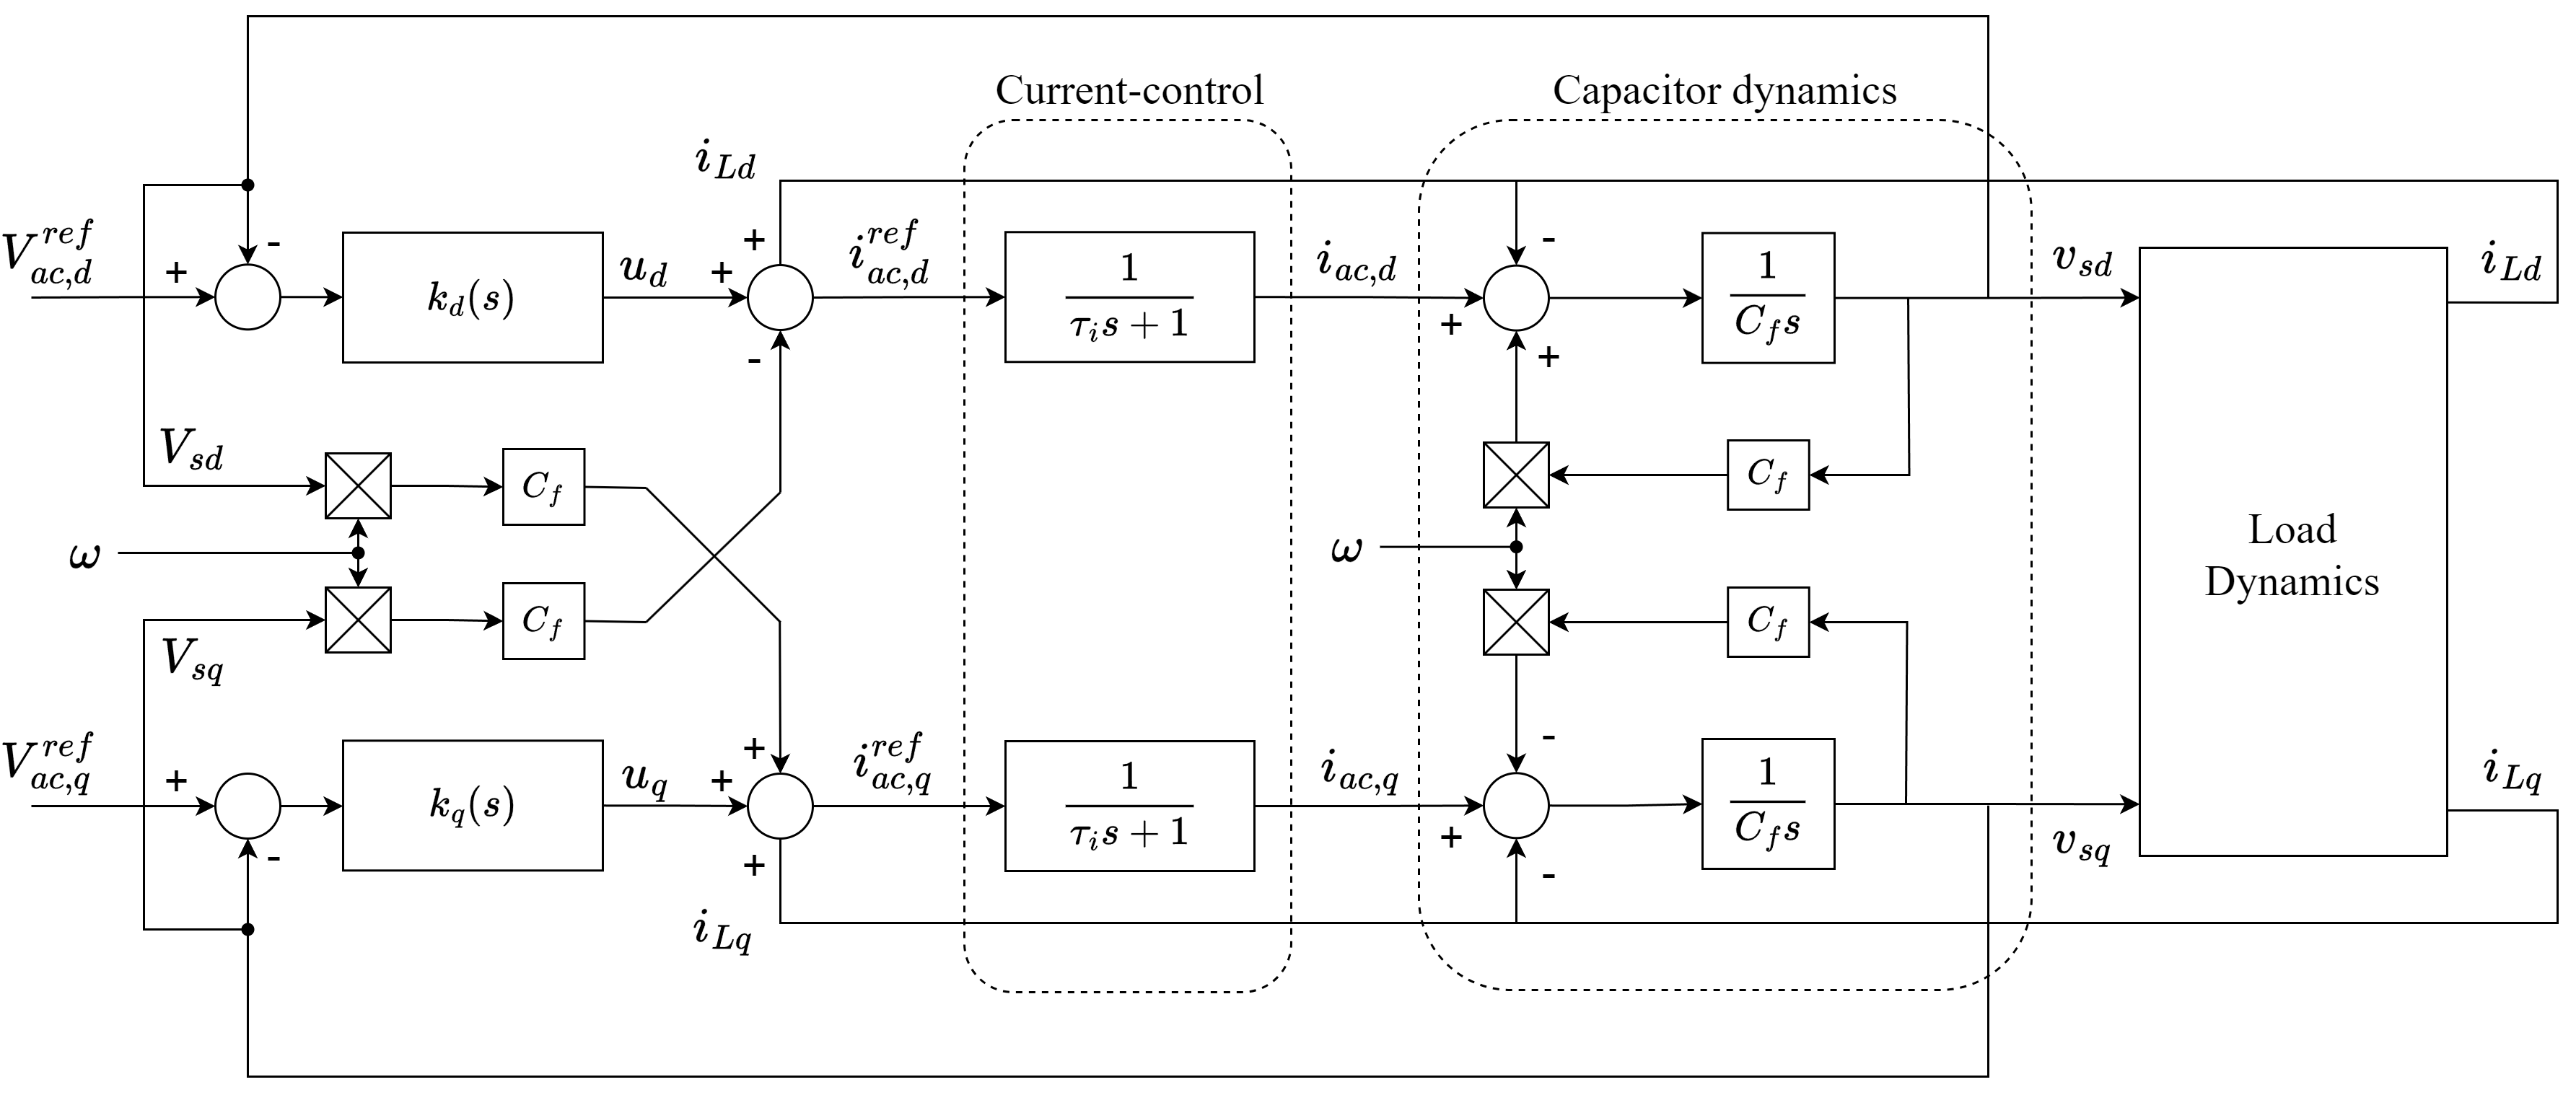
\includegraphics[width = 1\columnwidth]{inv_vc2.png}
    \caption{VSC grid-forming control diagram in the dq frame}
    \label{fig:inv_diagram_gfm}
\end{figure}

The first compensator can be processed as $e_d = V_{sdref}-V_{sd}$ and generates $u_d$. The other compensator processes $e_q = V_{sqref}-V_{sq}$ and generates $u_q$. Then $i_{dref}$ and $i_{qref}$ go to the corresponding current control loops on the $d$- and $q$ axes. The control diagram can be simplified to that of Figure~\cref{fig:inv_vc}.

\begin{figure}[htbp]
    \centering
    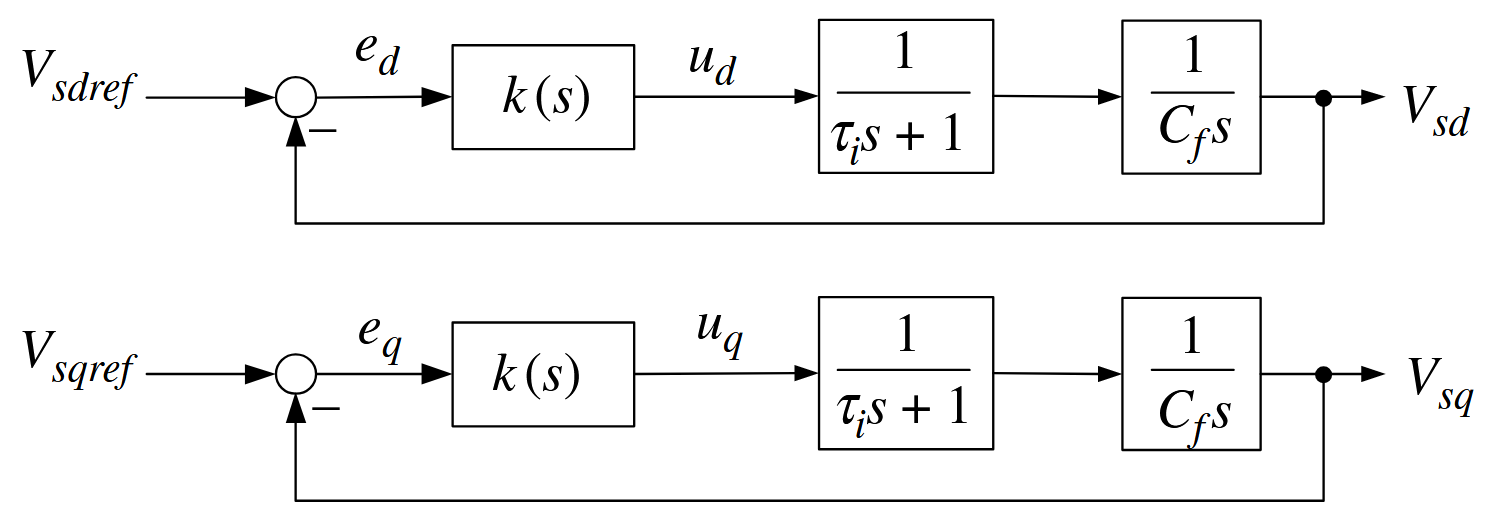
\includegraphics[width = 0.8\columnwidth]{inv_vc_pi.png}
    \caption{Simplified grid-forming control block diagram in the dq frame \autocite{book_yazdani_2010}}
    \label{fig:inv_vc}
\end{figure}

% \subsection{Parameters estimation}

\section{Transmission Lines}\label{sec:ch3/sec3}
Transmission lines (TL) are long conductors, suspended at a safe distance from the ground, in which the conductive wires are isolated from each other and from the external environment and protected by insulation and armor through which electrical energy is transmitted. TLs are characterized by a significant feature; they are elements with distributed length parameters. Accurate calculation of topologies containing such elements leads to complex calculations, so in practical calculations, power lines are often considered as elements with concentrated parameters. This assumption is valid for overhead lines up to 300-350 km and for underground cable lines up to 50-70 km \autocite{Gerasimenko2008}. The length of distributed electrical networks is significantly shorter, and they are often classified as local electrical networks, which can be considered objects with concentrated parameters in all cases \autocite{borovikov1977electric}. Thus, it can be assumed with sufficient accuracy that series resistance and series reactance are concentrated in the middle of the line, and conductance and susceptance are at the ends. These parameters can be deduced from the per-unit length resistance $R_L$, inductance $L_L$ and capacitance $C_L$ of the line \autocite{LIU2023109321}. So-called $\pi$-branch model can be used, which is represented in Figure~\cref{fig:pi_branch}. 

\begin{figure}[htbp]
    \centering
    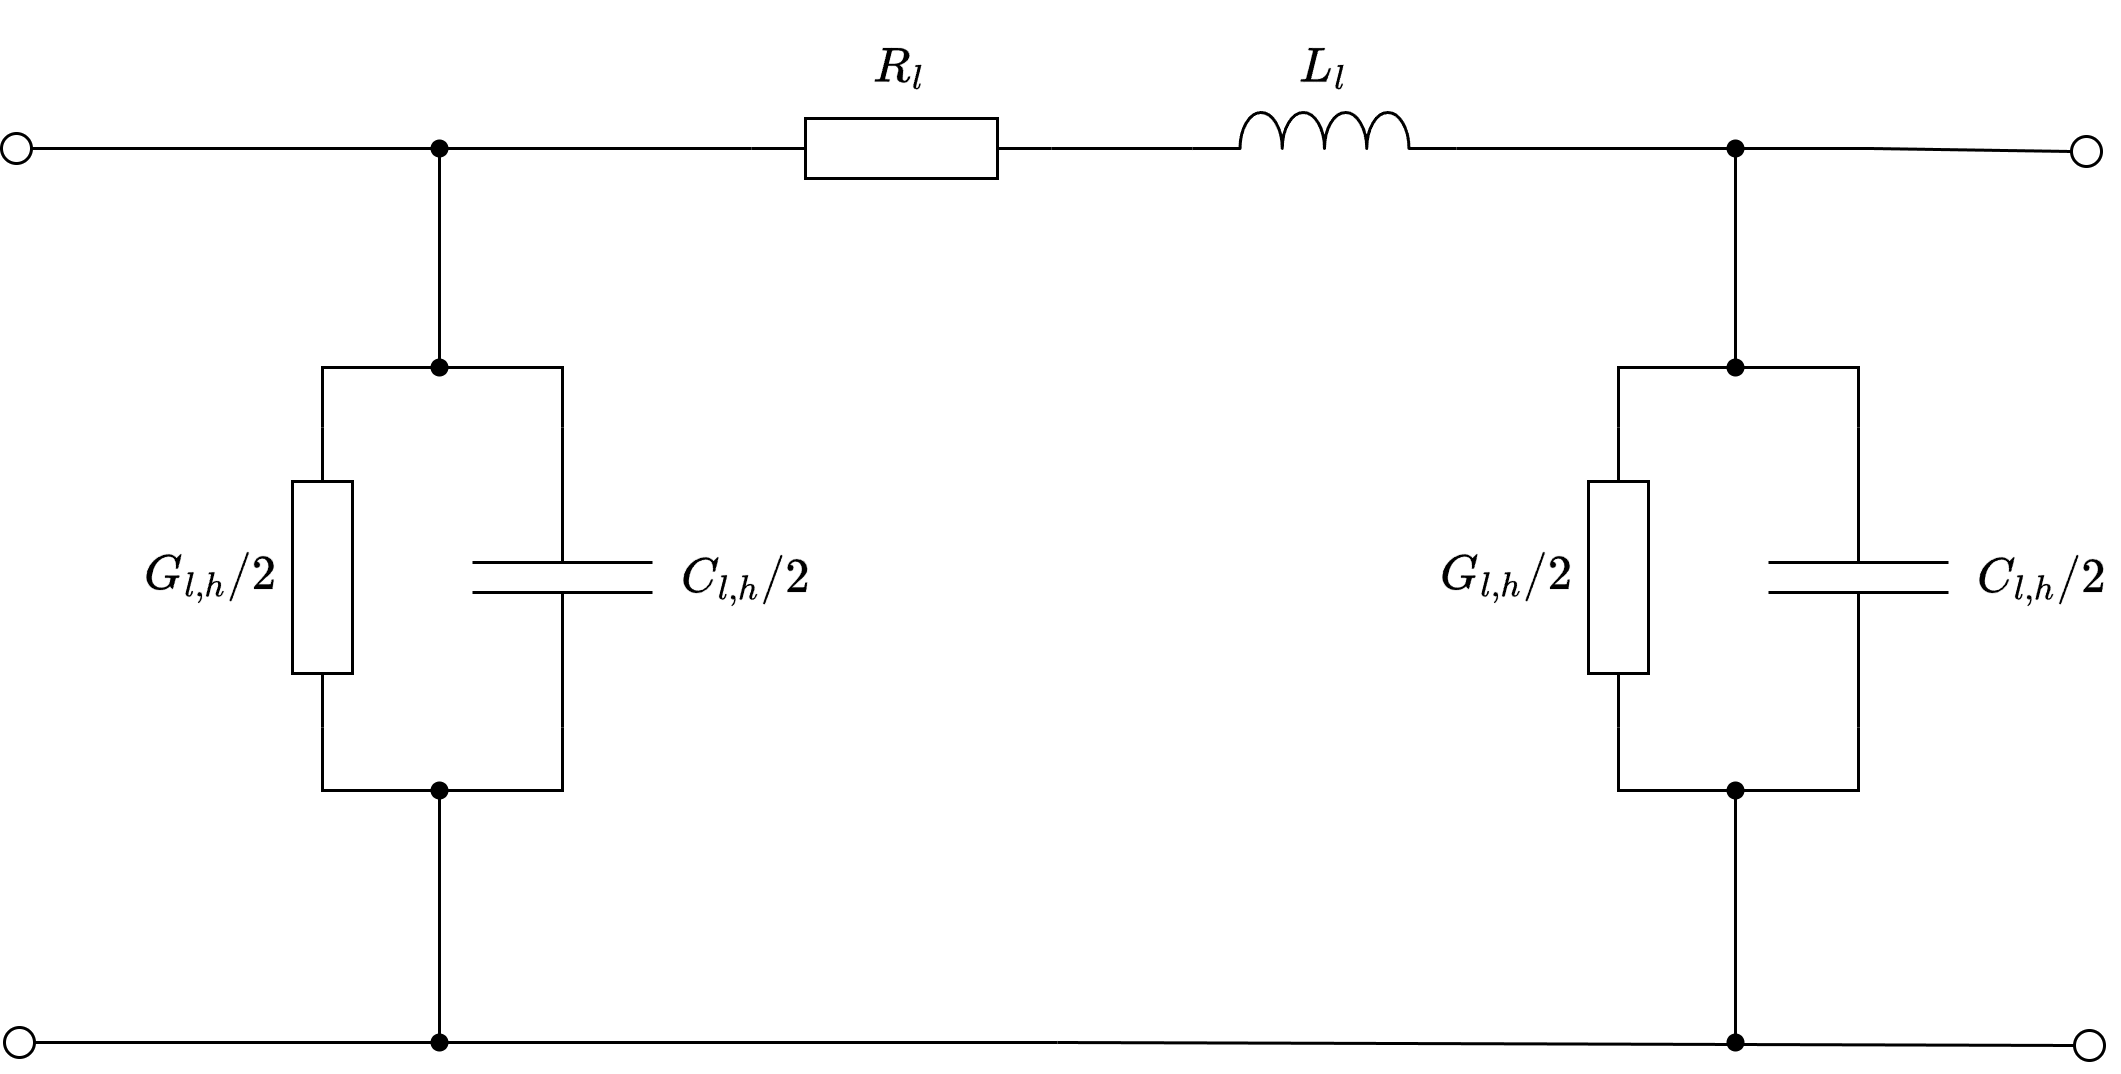
\includegraphics[width = 0.8\columnwidth]{PI-line.png}
    \caption{Line equivalent $\pi$-model with concentrated parameters}
    \label{fig:pi_branch}
\end{figure}

In the calculations of distribution electrical networks with a voltage of 0.38 to 35 kV, the replacement schemes shown in Figure~\cref{fig:pi_branch} are often simplified (the active and capacitive conductivities are not taken into account), and the scheme shown in Figure~\cref{fig:tl_04} is used. However, it should be noted that the use of simplified schemes, even in 10 to 35 kV networks, should be justified. For example, when modeling a single-phase ground fault in networks with an isolated or compensated neutral, it is not acceptable to neglect capacitive conductance. In this case, it is necessary to use the equivalent circuit shown in Figure~\cref{fig:tl_10}.

\subsection{Time domain scalar form single-section $\pi$-model with constant parameters}\label{subsec:ch3/sec3/sub1}
The model represent a single-section of $\pi$-model as shown in Figure~\cref{fig:tl_10}. 
\begin{figure}[htbp]
    \centering
    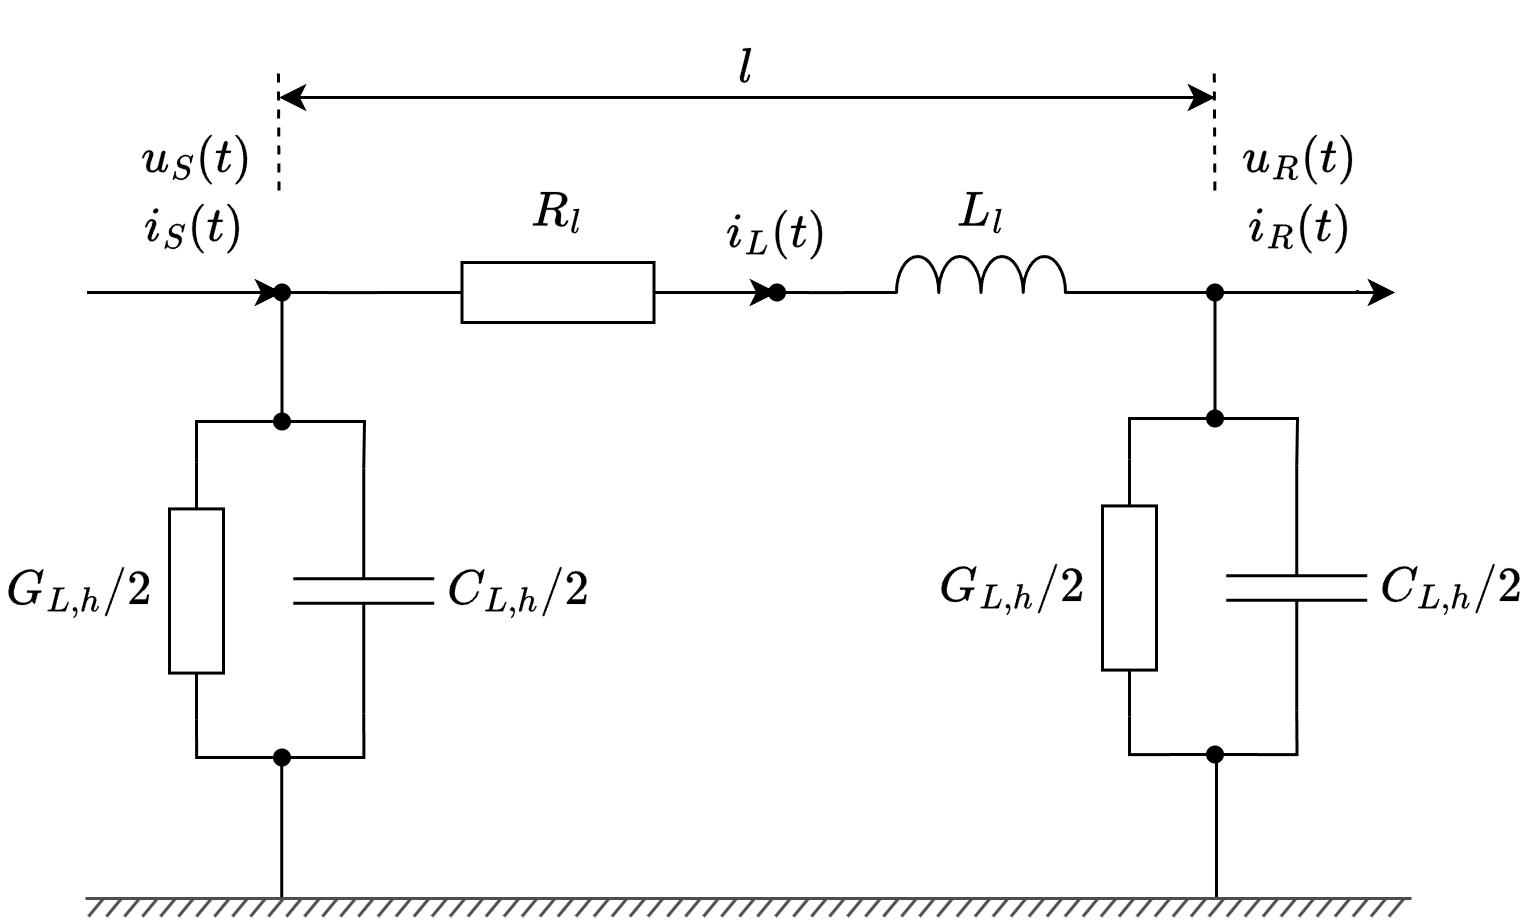
\includegraphics[width = 0.8\columnwidth]{TL_10.png}
    \caption{Equivalent circuit, time domain form single-section $\pi$ model with constant parameters}
    \label{fig:tl_10}
\end{figure}

The physical laws of this model can be described as \autocite{Liu2017TL, 9154583},
\begin{equation}
    \left\{\begin{array}{c}
        \displaystyle \mathbf{i}_{R}(t)=-\frac{\mathbf{G} l}{2} \mathbf{u}_{R}(t)-\frac{\mathbf{C} l}{2} \frac{d \mathbf{u}_{R}(t)}{d t}+\mathbf{i}_{L}(t) \\[1em]
        \displaystyle \mathbf{i}_{S}(t)=\frac{\mathbf{G} l}{2} \mathbf{u}_{S}(t)+\frac{\mathbf{C} l}{2} \frac{d \mathbf{u}_{S}(t)}{d t}+\mathbf{i}_{L}(t) \\[1em]
        \displaystyle \mathbf{0}=-\mathbf{u}_{S}(t)+\mathbf{u}_{R}(t)+\mathbf{R} l \mathbf{i}_{L}(t)+\mathbf{L} l \frac{d \mathbf{i}_{L}(t)}{d t}
    \end{array}\right.
\end{equation}
where the transmission line has a length of l. The terminal current and voltage vectors at the sending and receiving end are $i_S(t)$, $i_R(t)$, $u_S(t)$, and $u_R(t)$, respectively. Per unit length matrices for series resistance, inductance, shunt conductance, and capacitance are given by $R(x,t)$, $L(x,t)$, $G(x,t)$, and $C(x,t)$, respectively.

\subsection{Time domain scalar form RL model with constant parameters}\label{subsec:ch3/sec3/sub2}
Neglecting the shunt capacitance and conductance for a low voltage cases, an RL model is established as shown in Figure~\cref{fig:tl_04}. 
\begin{figure}[htbp]
    \centering
    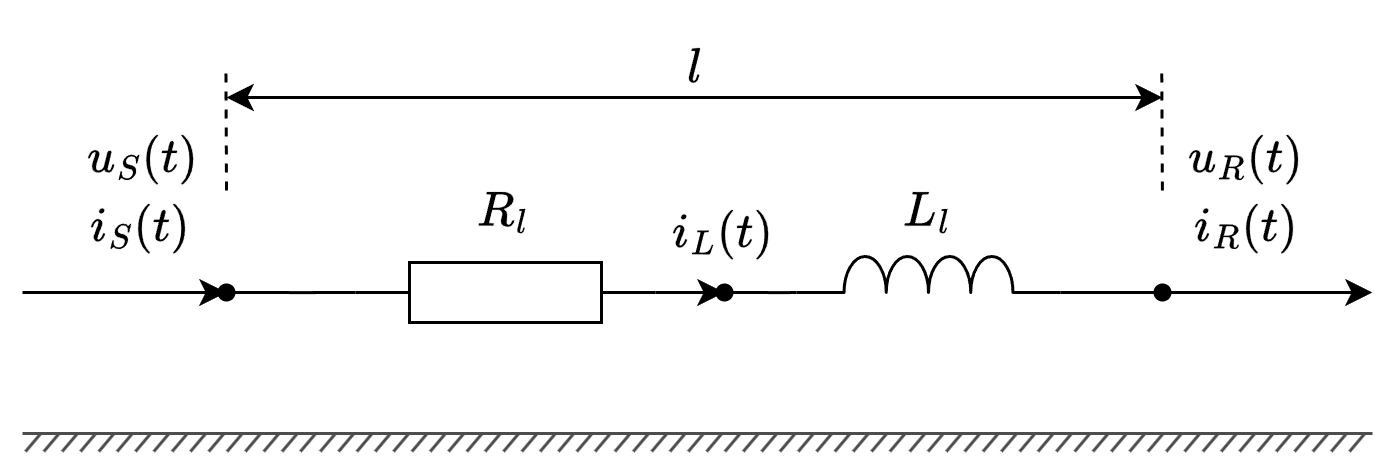
\includegraphics[width = 0.7\columnwidth]{TL_04.png}
    \caption{Equivalent circuit, time domain form RL model with constant parameters.}
    \label{fig:tl_04}
\end{figure}

The physical laws of this model can be described as \autocite{8811599},
\begin{equation}
    \left\{\begin{array}{c}
        \displaystyle \mathbf{i}_{R}(t)=\mathbf{i}_{L}(t), \quad \mathbf{i}_{S}(t)=\mathbf{i}_{L}(t), \\[1em]
        \displaystyle \mathbf{0}=-\mathbf{u}_{S}(t)+\mathbf{u}_{R}(t)+\mathbf{R} l \mathbf{i}_{L}(t)+\mathbf{L} l \frac{d \mathbf{i}_{L}(t)}{d t}.
    \end{array}\right.
\end{equation}

% \subsection{Parameters estimation}
% Several techniques have been described in the literature to estimate the parameters of the transmission line model from measurements. 

% \section{Power Transformer}

\section{Loads}\label{sec:ch3/sec4}
Prosumers, including storage systems and electric vehicles, can be modeled and integrated within the previously established current source framework, characterized by negative power generation. Conversely, the remaining $l$ loads are commonly modeled as voltage-dependent, with its active power $P$ and reactive power $Q$ adjusting according to changes in the positive sequence voltage \autocite{9369128}.
\begin{equation}\label{eq:pq_l}
    P_l = P_0(V/V_0)^\alpha, \quad Q_l = Q_0(V/V_0)^\beta,
\end{equation}

\noindent where $\alpha$ and $\beta$ are the coefficients for voltage in relation to active and reactive power, typically ranging from 0 to 2. When $\alpha = \beta = 0$, the load exhibits constant power characteristics; when $\alpha = \beta = 1$, the load behaves as a constant current source; and when $\alpha = \beta = 2$, the load acts as a constant impedance. The variable $V_0$ denotes the initial positive sequence voltage.

The initial operating point is defined by the active power $P_0$ and reactive power $Q_0$ at the initial voltage $V_0$. The active and reactive power, denoted by $P$ and $Q$, vary in accordance with the power reference provided by a measurement device, which is based on the positive sequence voltage $V$.

\section{Simulation engine}\label{sec:ch3/sec5}

In digital simulations carried out in the time domain, a system that operates continuously over time needs to be represented in a discrete form. Due to this transformation, it is not possible to directly derive or integrate the original continuous-time equations. Instead, the dynamic behavior of the system is approximated using suitable numerical techniques. To make this possible, the differential equations that describe continuous-time dynamics are rewritten as difference equations, which can then be solved step by step on a computer. The Electromagnetic Transients (EMT) simulation is widespread approach for generating this type of information \autocite{dommel1992emtp,4073845,osti_78239,277712,56581}, and is often used to validate steady-state power system analyses against transient simulations. Real-time EMT enhances DT's ability to model sensitive system operating conditions. 

% For example, for the case of an inductor, shown in Figure~\cref{fig:inductor},
% \begin{figure}[htbp]
%     \centering
%     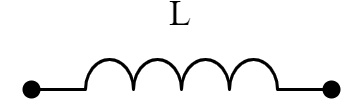
\includegraphics[width = 0.3\columnwidth]{graphics/inductor.png}
%     \caption{Inductor component}
%     \label{fig:inductor}
% \end{figure}
% the relation between the voltage across it and its current is given by
% \begin{equation}
%     V_{L}(t)=L \frac{d i_{L}(t)}{d t}
% \end{equation}

% Solving for the voltage,
% \begin{equation}
% \begin{aligned}
%     \begin{array}{c}
% \displaystyle V_{L} d t=L d i_{L}(t) \\[1em]
% \displaystyle \int_{t-\Delta t}^{t} V_{L} d t=L \int_{t-\Delta t}^{t} d i_{L}(t) \\[1em]
% \displaystyle \int_{t-\Delta t}^{t} V_{L} d t=L\left[i_{L}(t)-i_{L}(t-\Delta t)\right]
% \end{array}
% \end{aligned}
% \end{equation}
% where $\Delta t$ is the discretization time step. Approximating the left-hand side with the trapezoidal formula, we obtain
% \begin{equation}
%     \frac{V_{L}(t)+V_{L}(t-\Delta t)}{2} \Delta t=L\left[i_{L}(t)-i_{L}(t-\Delta t)\right]
% \end{equation}

% Then the voltage across the inductor is
% \begin{equation}
%     V_{L}(t)=\frac{2 L}{\Delta t} i_{L}(t)+\left[-V_{L}(t-\Delta t)-\frac{2 L}{\Delta t} i_{L}(t-\Delta t)\right]
%     \label{eq:l_discrete}
% \end{equation}

% Equation \eqref{eq:l_discrete} can be represented by the equivalent discrete time circuit of Figure~\cref{fig:inductor_discrete}.
% \begin{figure}[htbp]
%     \centering
%     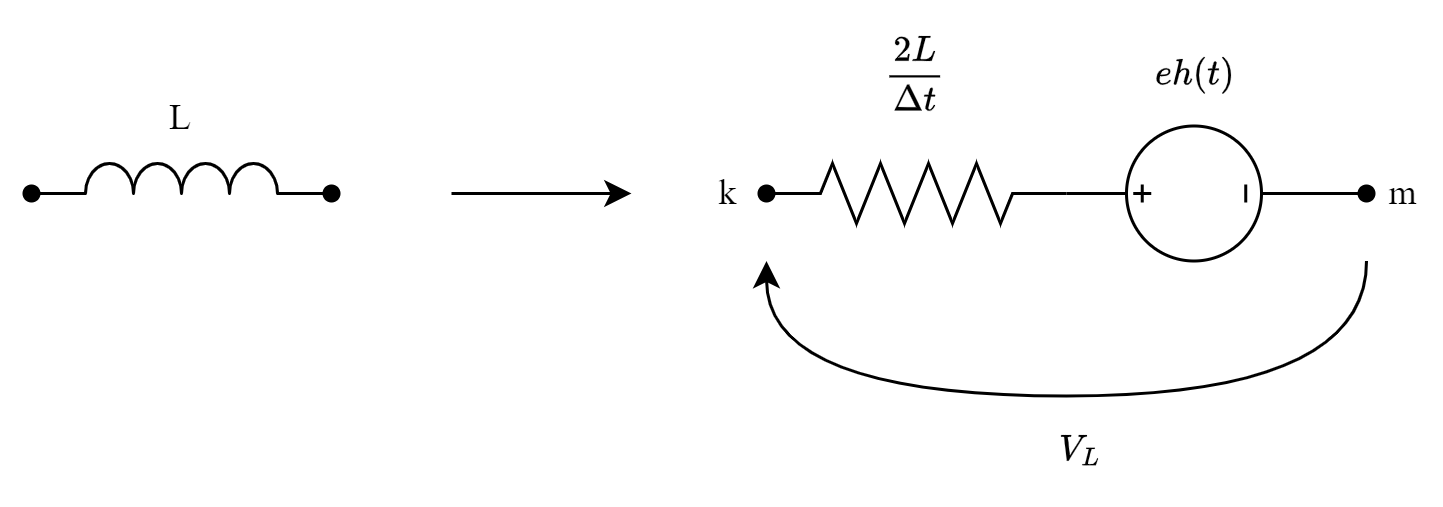
\includegraphics[width = 0.8\columnwidth]{graphics/inductor_discrete.png}
%     \caption{Inductor discrete time equivalent with trapezoidal rule}
%     \label{fig:inductor_discrete}
% \end{figure}

% \section{Discretization Rule Stability} ??????????????????????
\subsection{Nodal Analysis}\label{subsec:ch3/sec5/sub1}
The nodal analysis approach relies on Kirchhoff’s current law, which allows to obtain the voltage in each of the nodes of an electrical circuit. The general form is presented in a simplified form below:
\begin{equation}
    [G][V]=[I]
\end{equation}
where\\  
$G$ represents the $N \times N$ of nodal conductance,\\
$V$ is the vector of nodal voltages,\\  
$I$ are the known vector of current sources injected into the nodes, \\
$N$ is the number of nodes, excluding ground.

The matrix $[G]$ is real, symmetrical and unchanged unless switches or the time step $(\Delta t)$ will change. It is constructed like the nodal admittance matrix used in steady-state analysis. The equations system can be structured using partitioning methods for the nodal conductance matrix and voltage/current vectors:
\begin{equation}
    \left[\begin{array}{ll}
G_{AA} & G_{AB} \\
G_{BA} & G_{BB}
\end{array}\right]\left[\begin{array}{l}
V_{A} \\
V_{B}
\end{array}\right]=\left[\begin{array}{l}
I_{A} \\
I_{B}
\end{array}\right]
\end{equation}
where\\
$V_1$ is the vector of unknown nodal voltages;\\
$V_2$ is the vector of known nodal voltages, in nodes with connected voltage sources.

Then, to find the target node voltages, the Gaussian elimination method is used in the matrix system:
\begin{equation}
    G_{AA} V_{A}=J_{A}-Y_{AB} V_{B}
\end{equation}
Thus, we determine nodal voltages at time $t$, then increase $t$ by $\Delta t$, revise the vector on the right-hand side, and compute nodal voltages, branch voltages, and currents.

\subsection{Discrete Time State-Space Formulation}\label{subsec:ch3/sec5/sub2}
A Linear Time-Invariant (LTI) system can be formulated using discrete-time state-space equations, defined by inputs (external excitations), outputs (measurable quantities), and states (internal dynamics). State variables evolve as functions of past and present states and inputs, so the energy stored in the system at time $t$ is fully determined by the state. A state space representation of a system with multiple inputs and outputs can be visualized in a block diagram, shown in Figure~\cref{fig:ss_block}. 
\begin{figure}[htbp]
    \centering
    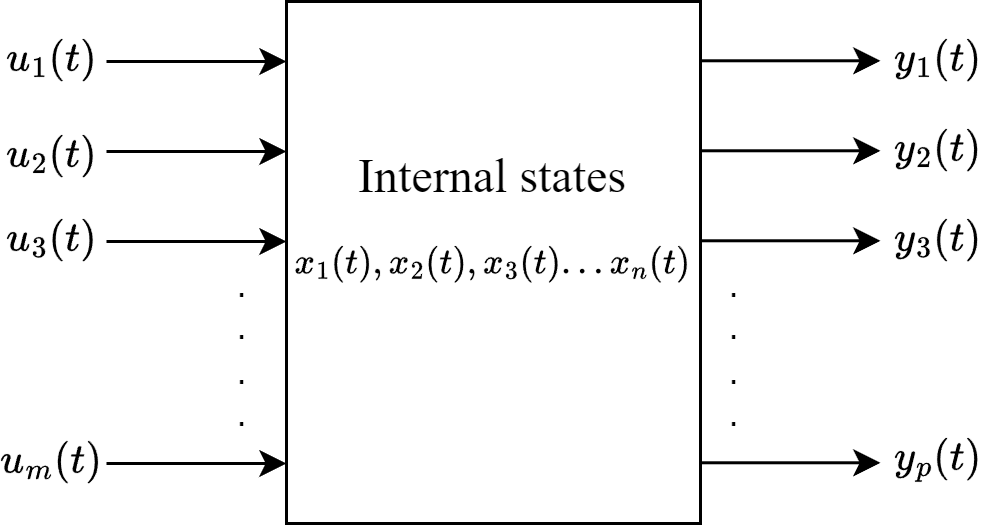
\includegraphics[width = 0.7\columnwidth]{ss_block.png}
    \caption{State-space representation of a multiple input/output system}
    \label{fig:ss_block}
\end{figure}

We consider $m$ inputs, $p$ outputs, and $n$ states. For a system described by $n$ first-order linear difference equations, a minimal state-space representation requires exactly $n$ internal states. At each discrete time instant $t$, the state variables can be expressed as a linear function of the previous state values and the corresponding input values at time $(t - \Delta t)$,
\begin{equation}
    \begin{aligned}
{\left[\begin{array}{c}
x_{1}(t) \\
\vdots \\
x_{n}(t)
\end{array}\right]=} & {\left[\begin{array}{ccc}
a_{11} & \ldots & a_{1 n} \\
\vdots & \ddots & \vdots \\
a_{n 1} & \ldots & a_{n n}
\end{array}\right]\left[\begin{array}{c}
x_{1}(t-\Delta t) \\
\vdots \\
x_{n}(t-\Delta t)
\end{array}\right]+} \\
& {\left[\begin{array}{ccc}
b_{11} & \ldots & b_{1 m} \\
\vdots & \ddots & \vdots \\
a_{n 1} & \ldots & a_{n m}
\end{array}\right]\left[\begin{array}{c}
u_{1}(t-\Delta t) \\
\vdots \\
u_{m}(t-\Delta t)
\end{array}\right] }
\end{aligned}
\label{eq:sv_xau}
\end{equation}

In discrete time $t$, the output variables can be formulated as linear combinations of the input and state variables evaluated at the same instant.
\begin{equation}
    \begin{aligned}
{\left[\begin{array}{c}
y_{1}(t) \\
\vdots \\
y_{p}(t)
\end{array}\right]=} & {\left[\begin{array}{ccc}
c_{11} & \ldots & c_{1 n} \\
\vdots & \ddots & \vdots \\
c_{p 1} & \ldots & c_{p n}
\end{array}\right]\left[\begin{array}{c}
x_{1}(t) \\
\vdots \\
x_{n}(t)
\end{array}\right]+} \\
& {\left[\begin{array}{ccc}
d_{11} & \ldots & d_{1 m} \\
\vdots & \ddots & \vdots \\
d_{p 1} & \ldots & d_{p m n}
\end{array}\right]\left[\begin{array}{c}
u_{1}(t) \\
\vdots \\
u_{m}(t)
\end{array}\right] }
\end{aligned}
\label{eq:sv_ycd}
\end{equation}

For a single input-output system (\ref{eq:sv_xau}) and (\ref{eq:sv_xau}) became
\begin{equation}
    \begin{array}{l}
x(t)=A x(t-\Delta t)+B u(t-\Delta t) \\
y(t)=C x(t)+D u(t)
\end{array}
\end{equation}

The values of a system’s states evolve over time, determined by its memory, the present input, and the structure of its interconnections. State variations may arise from external inputs or from the system’s own internal dynamics. When changes are driven by inputs, they are considered forced, whereas changes produced by internal dynamics reveal the inherent behavior of the system. The simplified state-space diagram, described mentioned interconnections, is presented in Figure~\cref{fig:ss_diagram}.  

\begin{figure}[htbp]
    \centering
    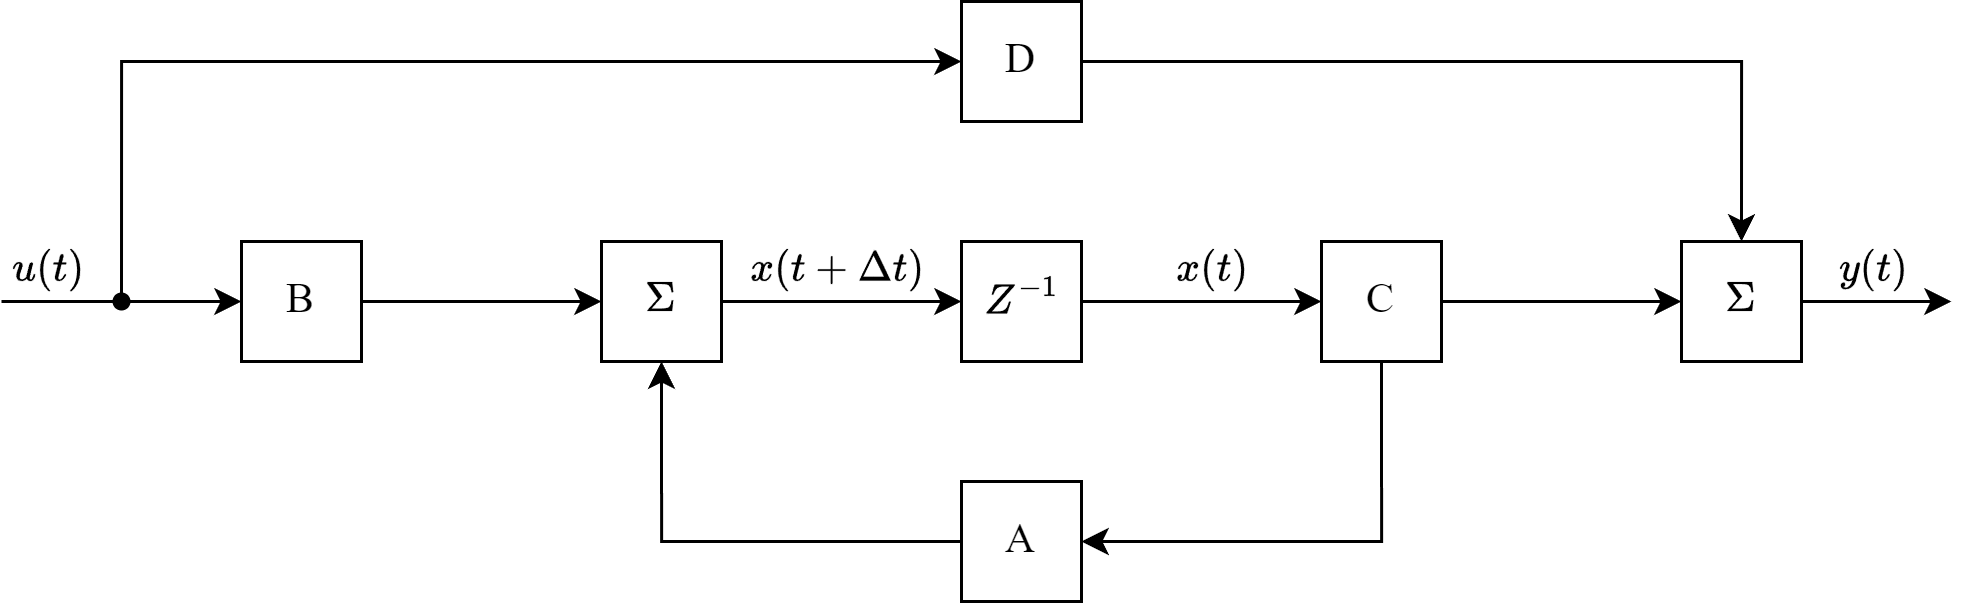
\includegraphics[width = 1\columnwidth]{ss_diagram.png}
    \caption{State-space representation of a multiple input/output system}
    \label{fig:ss_diagram}
\end{figure}

\subsection{EMTP Solution in Discrete Time State-Space form}\label{subsec:ch3/sec5/sub3}
According to the form of the nodal solution for EMTP \autocite{4073845},
\begin{equation}
    [G][v(t)]=[h(t)]+[u(t)]
    \label{eq:ns_emtp}
\end{equation}
Here, $[v(t)]$ denotes the nodal voltages, $[u(t)]$ represents the external current sources, $[G]$ is the nodal conductance matrix, and $[h(t)]$ corresponds to the vector of history sources. The system output can then be written as
\begin{equation}
    [v(t)]=[G]^{-1}[h(t)]+[G]^{-1}[u(t)]
\end{equation}

From historical sources prospective, the equation can be rewritten as
\begin{equation}
    [h(t+\Delta t)]=[A][h(t)]+[B][u(t)]
    \label{eq:ss_hyst}
\end{equation}

As shown, it connects the EMTP solutions with the preceding state idea in the state-space formulation, where the vector $[h(t)]$ represents the history sources as the system memory. This memory combines the system's prior behavior $h(t - \Delta t)$ with the input-influenced dynamics $u(t - \Delta t)$ and aligns well with the state-space definition. The EMTP solution updates $[h(t)]$ in terms of $[h(t - \Delta t)]$  and external current sources (\ref{eq:ss_hyst}), which exactly follows the form (\ref{eq:sv_xau}) of the state-space formulation. This approach describes branch history terms as the states within the electrical network, involving all the necessary information from the EMTP nodal solution and case data input \autocite{rowell1997system}.

\subsection{Discrete Time State-Space Model of the Elements}\label{subsec:ch3/sec5/sub4}
The EMT solution first defines the discretizations at the element level instead of discretizing the entire set of differential equations that describe the behavior of the network \autocite{Linares_Rojas_2001}. Consequently, in the EMT every component relationship between its current and voltage is modeled with a discrete-time equivalent. These difference equations are represented by discrete-time equivalent circuits consisting of resistance and source combinations.

\textbf{Resistance R}. Considering that the resistor is a linear and time-invariant element, the relationship between the voltage at its terminals and the current that flows through it is given by an algebraic equation.
\begin{equation}
    v(t)=Ri(t)
\end{equation}
where
\begin{equation}
    \begin{array}{c}
v(t)=v_{k m}(t)=e_{k}(t)-e_{m}(t), \\
i(t)=i_{k m}(t).
\end{array}
\end{equation}

Thus, the discrete equivalent circuit model of the resistor is itself, as shown in Figure~\cref{fig:emt_r}. In this case $h_{km}(t) = 0$ for all $t$. While resistive components lack branch history and thus do not contribute to the state, they offer damping.

\begin{figure}[htbp]
    \centering
    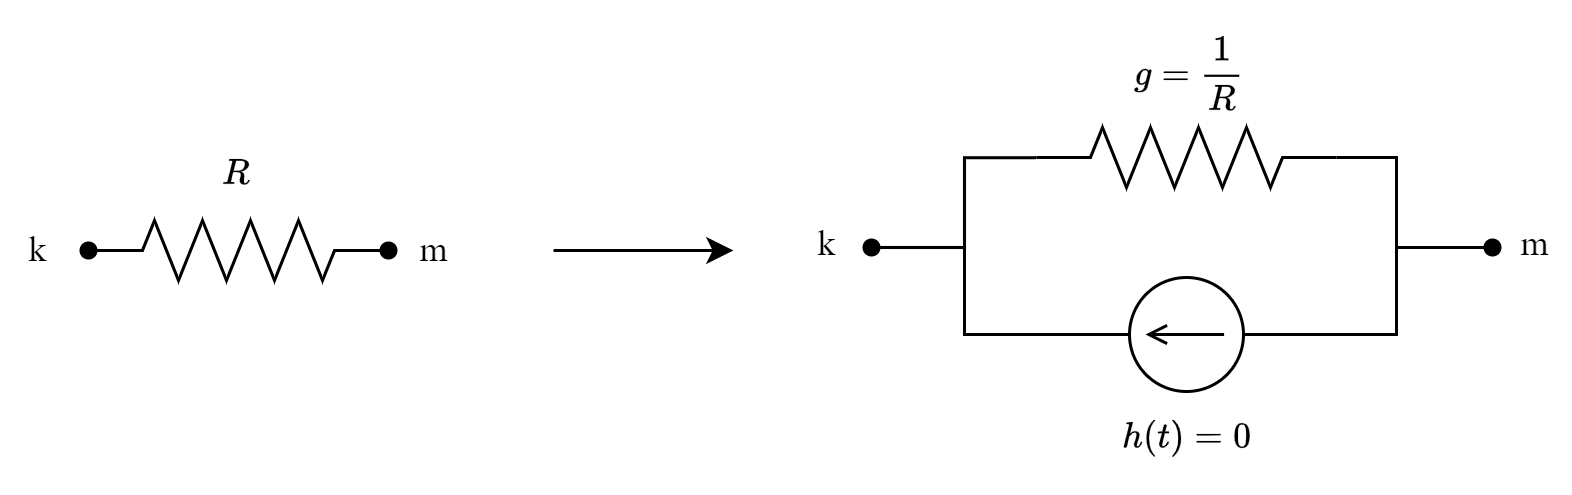
\includegraphics[width = 0.8\columnwidth]{emt_r.png}
    \caption{Discrete equivalent of a resistive element}
    \label{fig:emt_r}
\end{figure}

\textbf{Inductance L}
The discretized inductance is used to model single phase $\pi$-line equivalent, shunt reactors, inductive equivalent parts for loads, and other parts of equivalent circuits. The voltage-current relationship of the element is described by its characteristic equation:
\begin{equation}
    v(t)=L \frac{d i(t)}{d t} .
\end{equation}
Solving for the voltage,
\begin{equation}
\begin{aligned}
    \begin{array}{c}
\displaystyle V_{L} d t=L d i_{L}(t), \\[1em]
\displaystyle \int_{t-\Delta t}^{t} V_{L} d t=L \int_{t-\Delta t}^{t} d i_{L}(t), \\[1em]
\displaystyle \int_{t-\Delta t}^{t} V_{L} d t=L\left[i_{L}(t)-i_{L}(t-\Delta t)\right].
\end{array}
\end{aligned}
\end{equation}
where $\Delta t$ is the discretization time step. Approximating the left-hand side with the trapezoidal formula, we obtain
\begin{equation}
    \frac{V_{L}(t)+V_{L}(t-\Delta t)}{2} \Delta t=L\left[i_{L}(t)-i_{L}(t-\Delta t)\right],
\end{equation}

To obtain the Norton Equivalent Digital Model or the inductor in the discrete time, isolating $i(t)-i(t-\Delta t)$ formula should be converted to:
\begin{equation}
    i(t)-i(\mathrm{t}-\Delta \mathrm{t})=\frac{\Delta t}{2 L} v(t)+\frac{\Delta t}{2 L} v(t-\Delta \mathrm{t}).
\end{equation}
For $i(t)$, we have:
\begin{equation}
    i(t)=\frac{\Delta t}{2 L} v(t)+\frac{\Delta t}{2 L} v(t-\Delta \mathrm{t})+i(t-\Delta t),
\end{equation}
where,
\begin{equation}
    i h_{L}(t)=\left[i(t-\Delta t)+\frac{\Delta t}{2 L} v(t-\Delta t)\right].
    \label{eq:ihl}
\end{equation}

Thus,
\begin{equation}
    i(t)=\frac{\Delta t}{2 L} v(t)+i h_{L}(t).
\end{equation}

To ensure consistent source conversion with the Thévenin Equivalent Digital Model's voltage polarity, the sign in Eq. (\ref{eq:ihl}) giving a form, shown in Figure~\cref{fig:l_eqv2}.
\begin{equation}
\begin{array}{c}
    \displaystyle i h_{L}(t)=\left[-i(t-\Delta t)-\frac{\Delta t}{2 L} v(t-\Delta t)\right],\\[1em]
    \displaystyle i(t)=\frac{\Delta t}{2 L} v(t)-i h_{L}(t).
    \end{array}
\end{equation}

The inductance in Figure~\cref{fig:l_eqv2}'s equivalent circuit represented as a digital resistance $\frac{2 L}{\Delta t}$, paralleled by a historical current source $(ih(t))$, accounting for past data, as it inputs values from prior intervals into the current time step \autocite{de2022introduction}.

\begin{figure}[htbp]
    \centering
    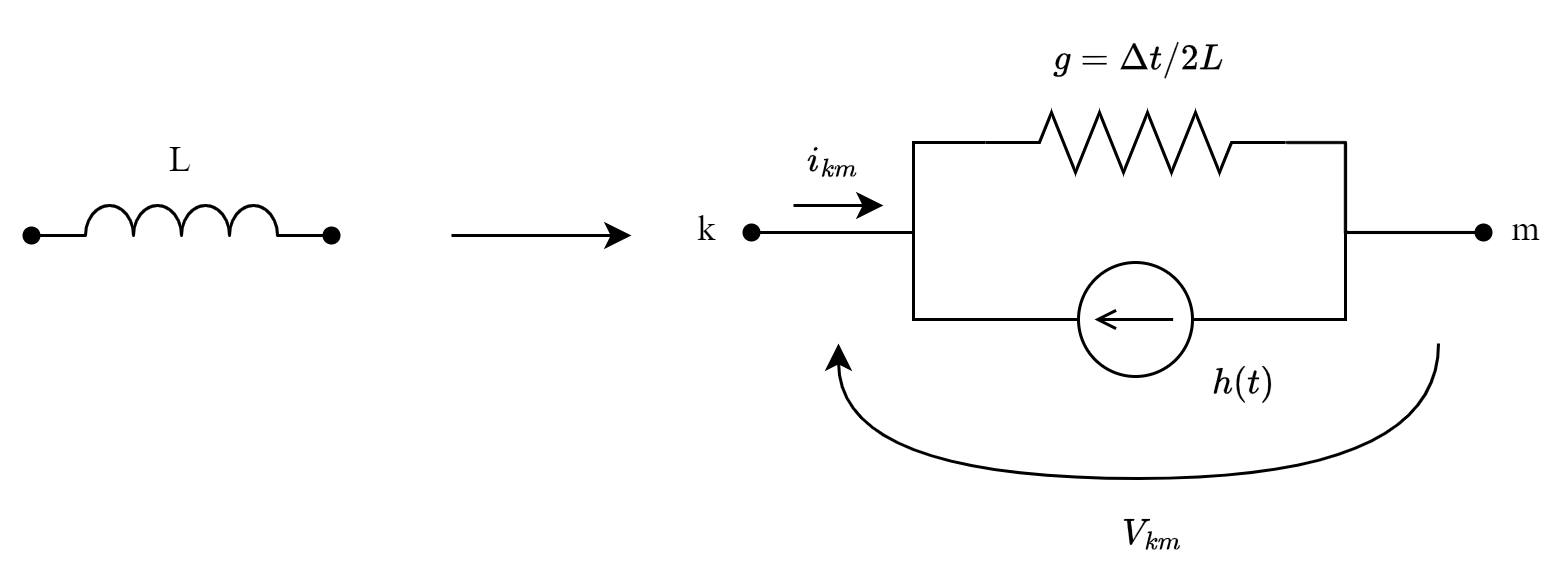
\includegraphics[width = 0.8\columnwidth]{l_eqv2.png}
    \caption{Discrete equivalent of a inductive element}
    \label{fig:l_eqv2}
\end{figure}

\textbf{Capacitance C}. The discretized capacitance generally models series and shunt capacitors in $\pi$-circuit transmission lines, converter parts like filters, capacitance transformers, capacitive dividers, and stray capacitance in generators, particularly for transient recovery voltage and lightning analyzes.

The characteristic equation that outlines the behavior of this element describes the connection between the current flowing through it and the voltage across its terminals:
\begin{equation}
    i(t)=C \frac{d v(t)}{d t}
\end{equation}
Solving for the current,
\begin{equation}
\begin{array}{c}
    \displaystyle i(t) d t=C d v(t),\\[1em]
    \displaystyle \int_{t-\Delta t}^{t} i(\tau) d \tau=C \int_{t-\Delta t}^{t} d v(\tau).
    \label{eq:c_current}
    \end{array}
\end{equation}

Using the trapezoidal rule on Eq. $(\ref{eq:c_current})$ converts the integral-differential form into an algebraic equation, enabling the development of a discrete capacitor model over time as follows:
\begin{equation}
    i(t)=\frac{2 C}{\Delta t} v(t)-i h_{C}(t).
\end{equation}

Thus, we have the Norton Equivalent Digital Model for the capacitor in the discrete time, shown in Figure~\cref{fig:c_eqv}:

\begin{figure}[htbp]
    \centering
    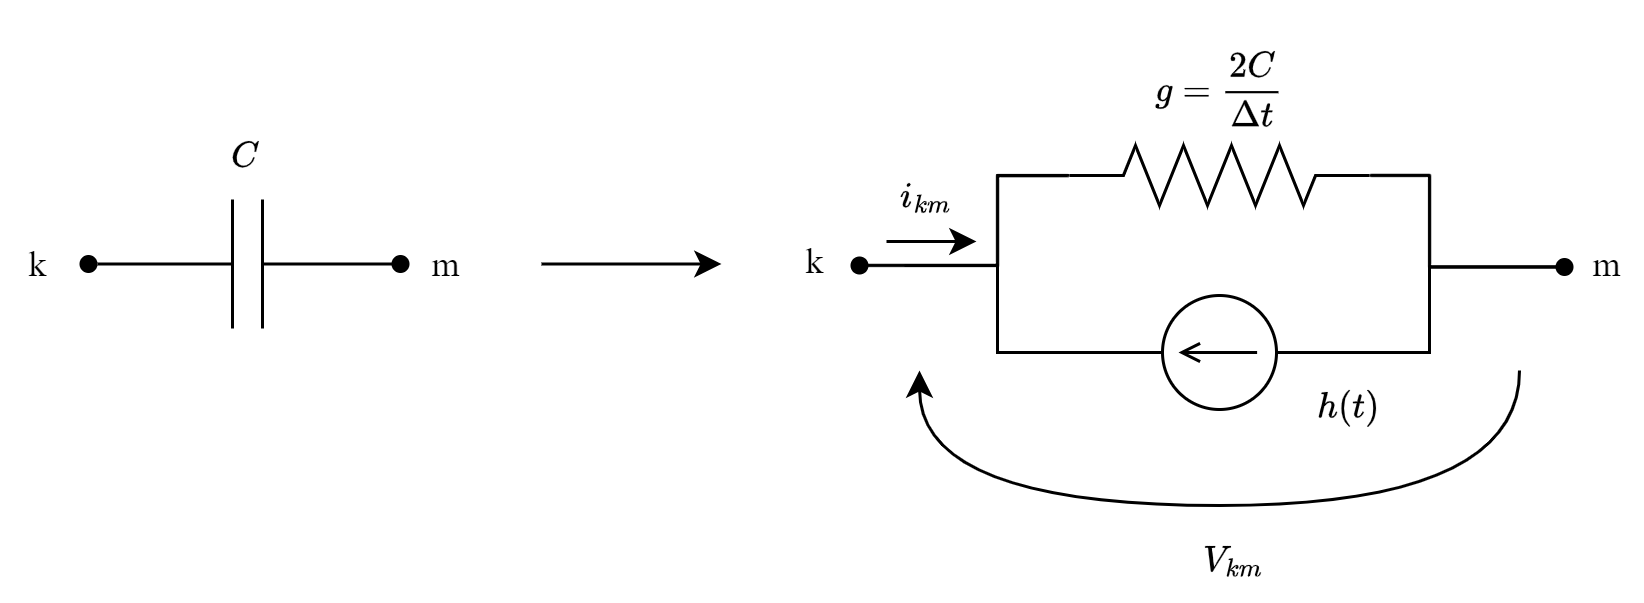
\includegraphics[width = 0.8\columnwidth]{c_eqv.png}
    \caption{Discrete equivalent of a capacitive element}
    \label{fig:c_eqv}
\end{figure}

Observing the equivalent circuit of Figure~\cref{fig:c_eqv}, the capacitance is modeled as an equivalent digital resistance $\Delta t/2C$ alongside a historical current source $(ih(t))$. This source includes past data since it adds values from the prior interval at each new time step.

\textbf{Treatment of Series Connection RL and RC}. The series connection of a resistor and inductor ($RL$) or series pair of resistor and capacitor ($RC$) can be modeled as a single equivalent discrete component. This combined representation accounts for the damping effect of the resistor and enhances computational efficiency by reducing both the number of nodes and branches in the system. The aggregation form of a resistor in series with an inductor is illustrated in Figure~\cref{fig:RL_eqv}.

\begin{figure}[htbp]
    \centering
    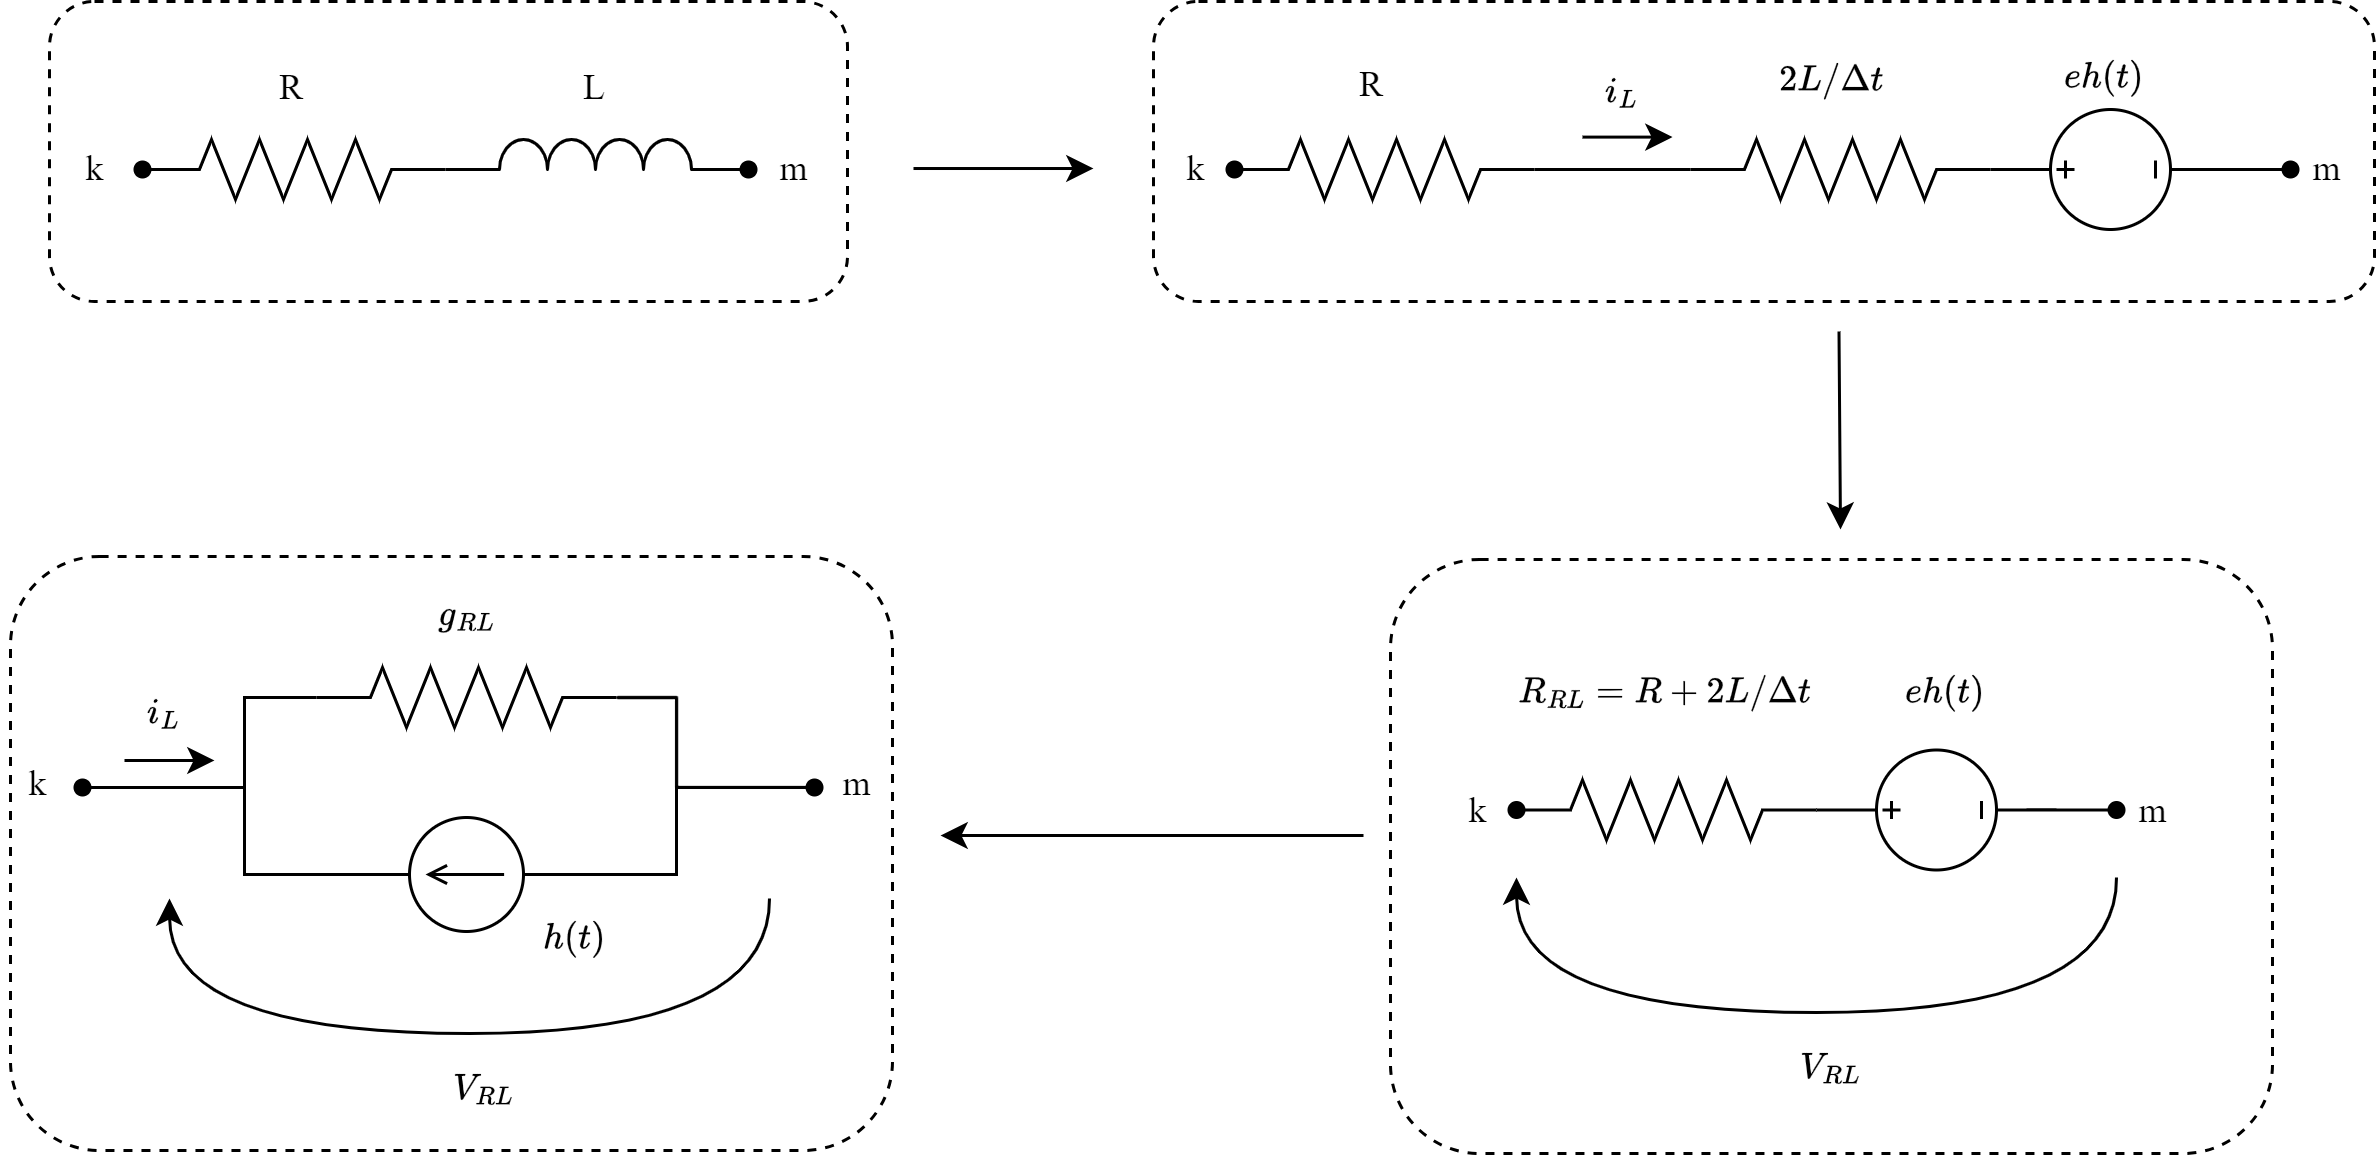
\includegraphics[width = 1\columnwidth]{RL_eqv.png}
    \caption{Discrete equivalent of a capacitive element}
    \label{fig:RL_eqv}
\end{figure}

Here, the connection ($RL$) and ($RC$) is kept respectively, 
\begin{equation}
    \begin{array}{c}
        h_{k m}(t)=h_{k m}(t-\Delta t)-2 g_{R L} v_{k m}(t-\Delta t),\\
        h_{k m}(t)=-h_{k m}(t-\Delta t)+2 g_{R C} v_{k m}(t-\Delta t)
    \end{array}
\end{equation}
where,
\begin{equation}
    g_{R L}=\frac{1}{R+\frac{2 L}{\Delta t}}, \hspace{1em}
    g_{R C}=\frac{1}{R+\frac{\Delta t}{2 C}}
\end{equation}

\textbf{Segmentation of Complex Network}. To provide computational efficiency of the simulation core in real-time for a case with many IBRs connected to the grid, above analysis with EMTP discrete time solutions can be introduced with the Multi-Area Thevenin Equivalent (MATE) concept \autocite{Hollman_2006}. The MATE concept was introduced for handling large power system networks in real-time dynamic studies \autocite{Linares_Rojas_2001, 729230}. The idea is to segment a complex network into independent subnets interconnected by links, as shown in Figure~\cref{fig:mate}. 

\begin{figure}[htbp]
    \centering
    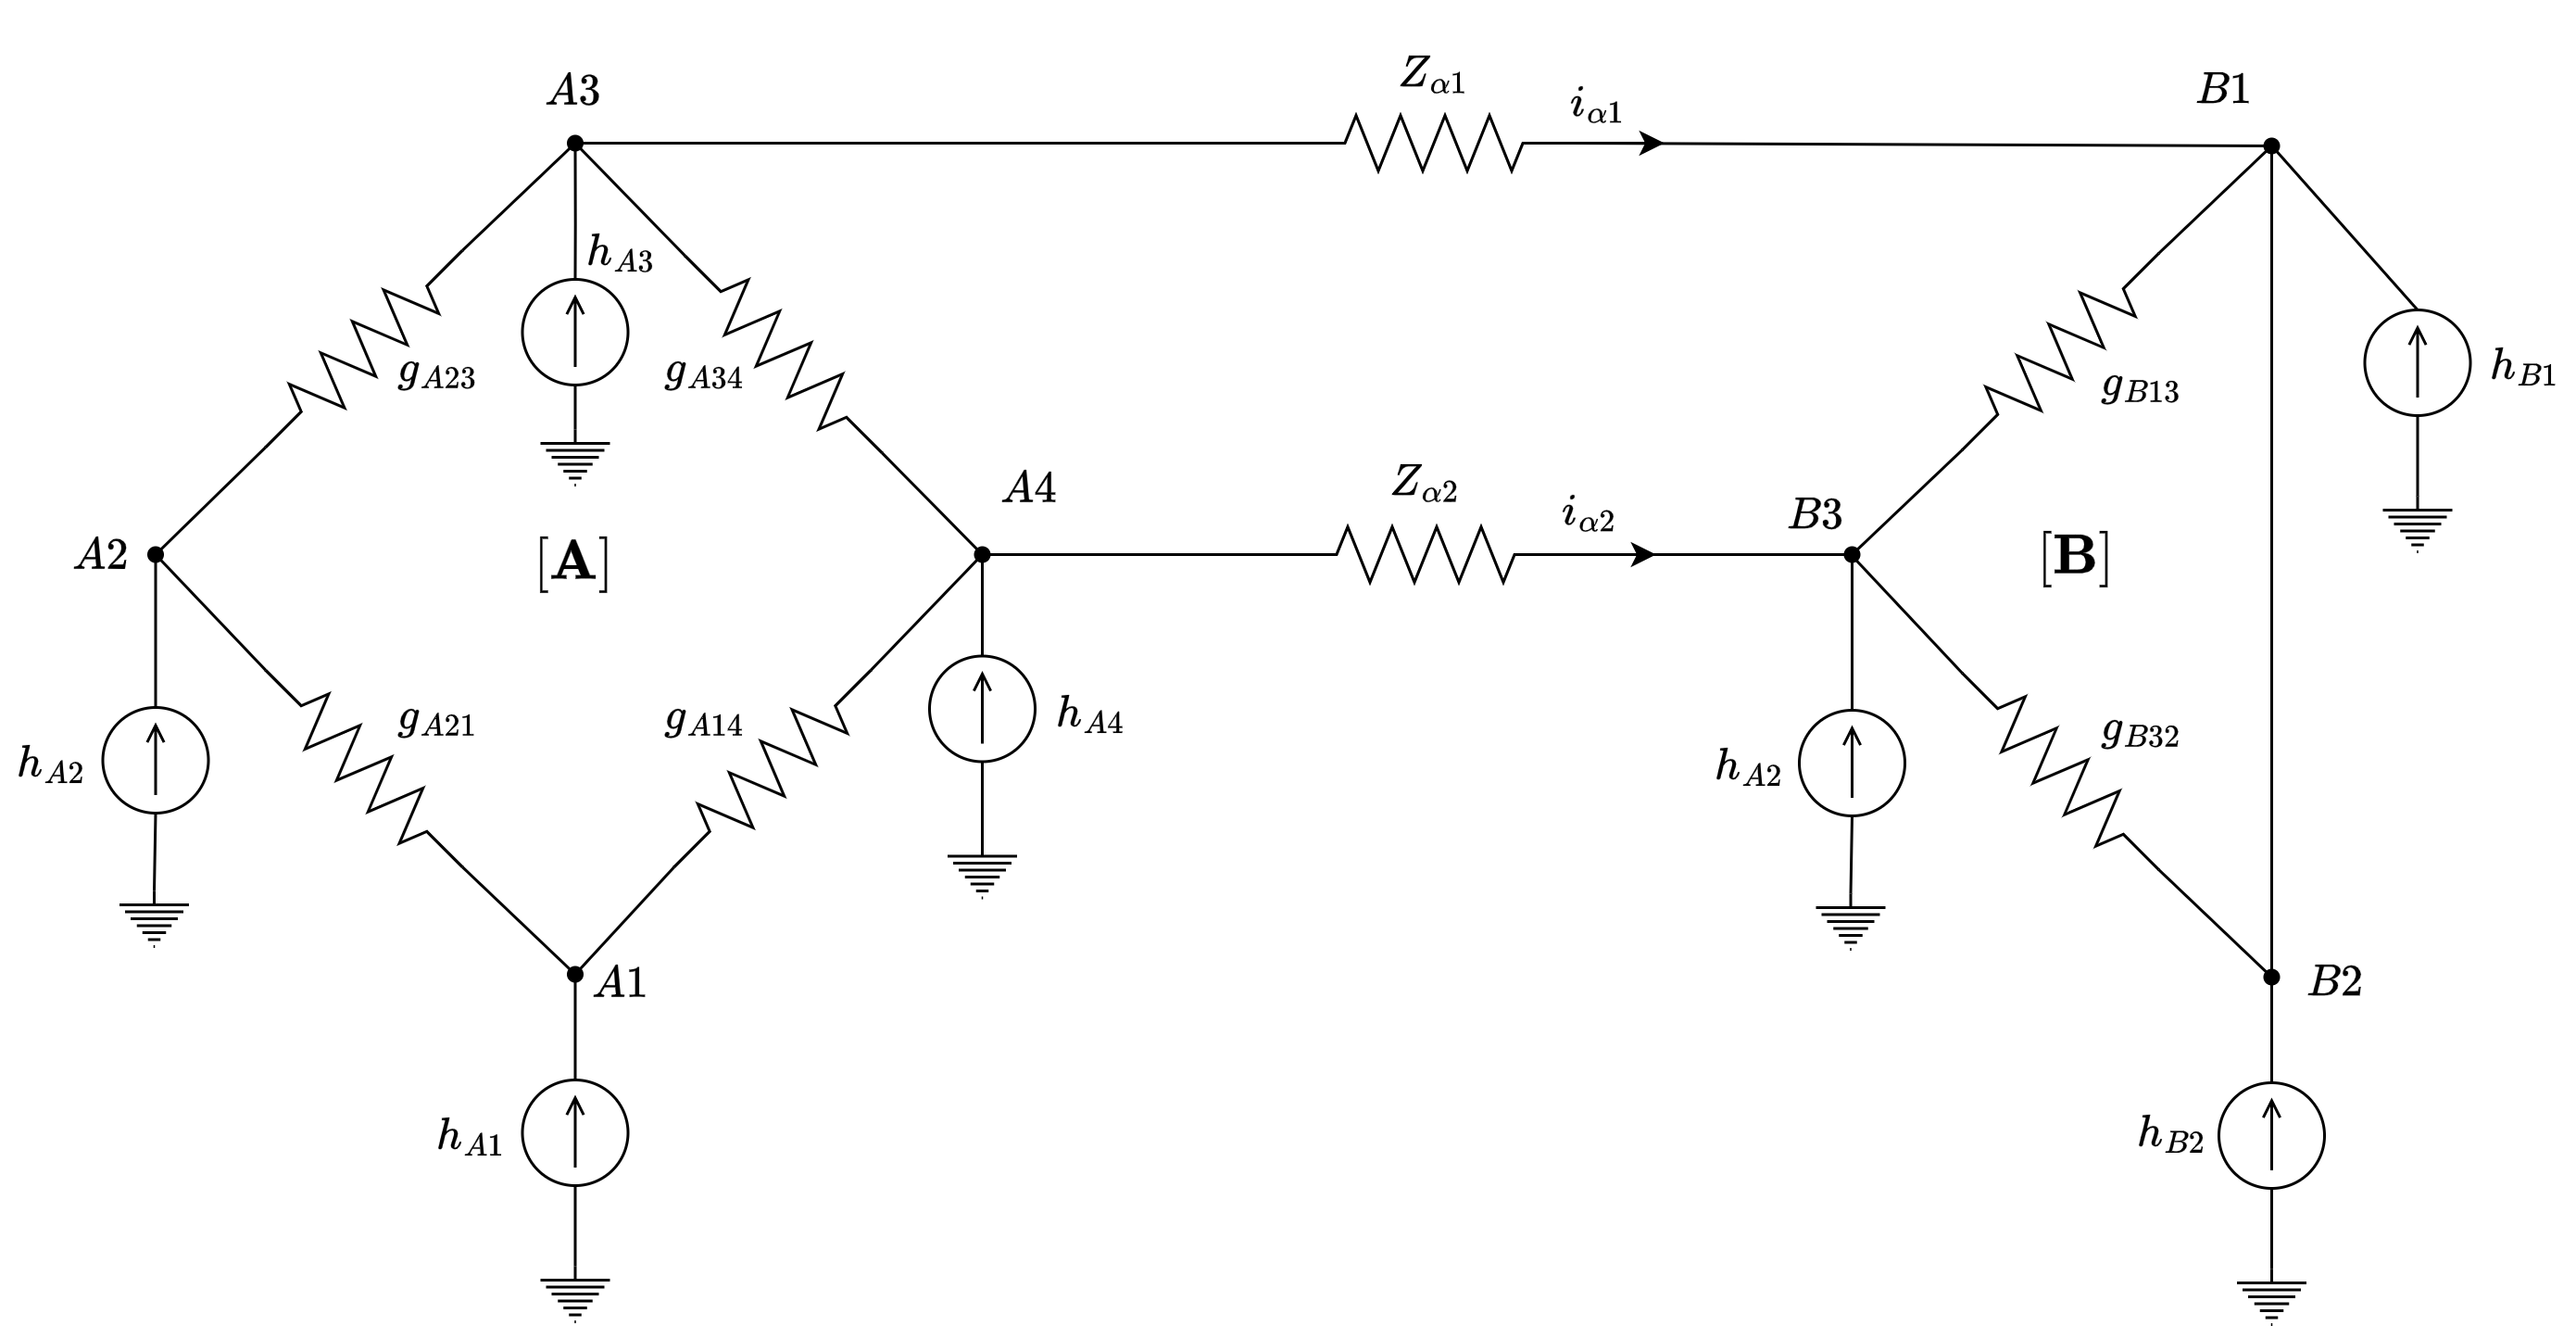
\includegraphics[width = 1\columnwidth]{mate.png}
    \caption{Circuit for discrete state-space MATE explanation \autocite{Mart2002OVNIIS}}
    \label{fig:mate}
\end{figure}

The general nodal equation of the system without the links $\alpha_1$ and $\alpha_2$ is,
\begin{equation}
    \left[\begin{array}{l|l}
A & 0 \\
\hline 0 & B
\end{array}\right]\left[\begin{array}{l}
v_{A} \\
\hline v_{B}
\end{array}\right]=\left[\begin{array}{l}
h_{A} \\
\hline h_{B}
\end{array}\right]
\end{equation}

\setlength{\arraycolsep}{3pt}
\begin{equation}
    \left[\begin{array}{cccc|ccc|cc}
G_{A 11} & G_{A 12} & 0 & G_{A 14} & & & & 0 & 0 \\
G_{A 21} & G_{A 22} & G_{A 23} & & & & & 0 & 0 \\
G_{A 31} & G_{A 32} & G_{A 33} & G_{A 34} & & & & 1 & 0 \\
G_{A 41} & 0 & G_{A 34} & G_{A 44} & & & & 0 & 1 \\
\hline & & & & G_{B 11} & G_{B 12} & G_{B 13} & -1 & 0 \\
& & & & G_{B 21} & G_{B 22} & G_{B 23} & 0 & 0 \\
& & & & G_{B 31} & G_{B 32} & G_{B 33} & 0 & -1 \\
\hline 0 & 0 & 1 & 0 & -1 & 0 & 0 & -z_{1} & 0 \\
0 & 0 & 0 & 1 & 0 & 0 & -1 & 0 & -z_{2}
\end{array}\right]\left[\begin{array}{c}
v_{A 1} \\
v_{A 2} \\
v_{A 3} \\
v_{A 4} \\
\hline v_{B 1} \\
v_{B 2} \\
v_{B 3} \\
\hline i_{\alpha 1} \\
i_{\alpha 2}
\end{array}\right]=\left[\begin{array}{c}
h_{A 1} \\
h_{A 2} \\
h_{A 3} \\
h_{A 4} \\
\hline h_{B 1} \\
h_{B 2} \\
h_{B 3} \\
\hline 0 \\
0
\end{array}\right]
\end{equation}
or it's compact notation,
\begin{equation}
    \left[\begin{array}{c|c|c}
A & 0 & p \\
\hline 0 & B & q \\
\hline p^{t} & q^{t} & -z
\end{array}\right]\left[\begin{array}{c}
v_{A} \\
\hline v_{B} \\
\hline i_{\alpha}
\end{array}\right]=\left[\begin{array}{c}
h_{A} \\
\hline h_{B} \\
\hline 0
\end{array}\right]
\end{equation}
with $[p]$ and $[q]$ as injection matrices from link branches.

This approach divide equivalent circuit into subnetwork nodes, with each node containing necessary information to formulate the discrete state-space equations. All discrete state-space description aggregates by central solver. The process of constructing the discrete state-space formulation of the network can be achieved at once, together with the case preprocessing stage. Only those subnetworks in which there is a topology change have to submit to the central solver the updated discrete state-space formulation \autocite{Hollman_2006}. This is particularly efficient for multicore real-time simulation, since the computation size of the circuit is reduced, as shown in Figure~\cref{fig:mate_mc}.

\begin{figure}[htbp]
    \centering
    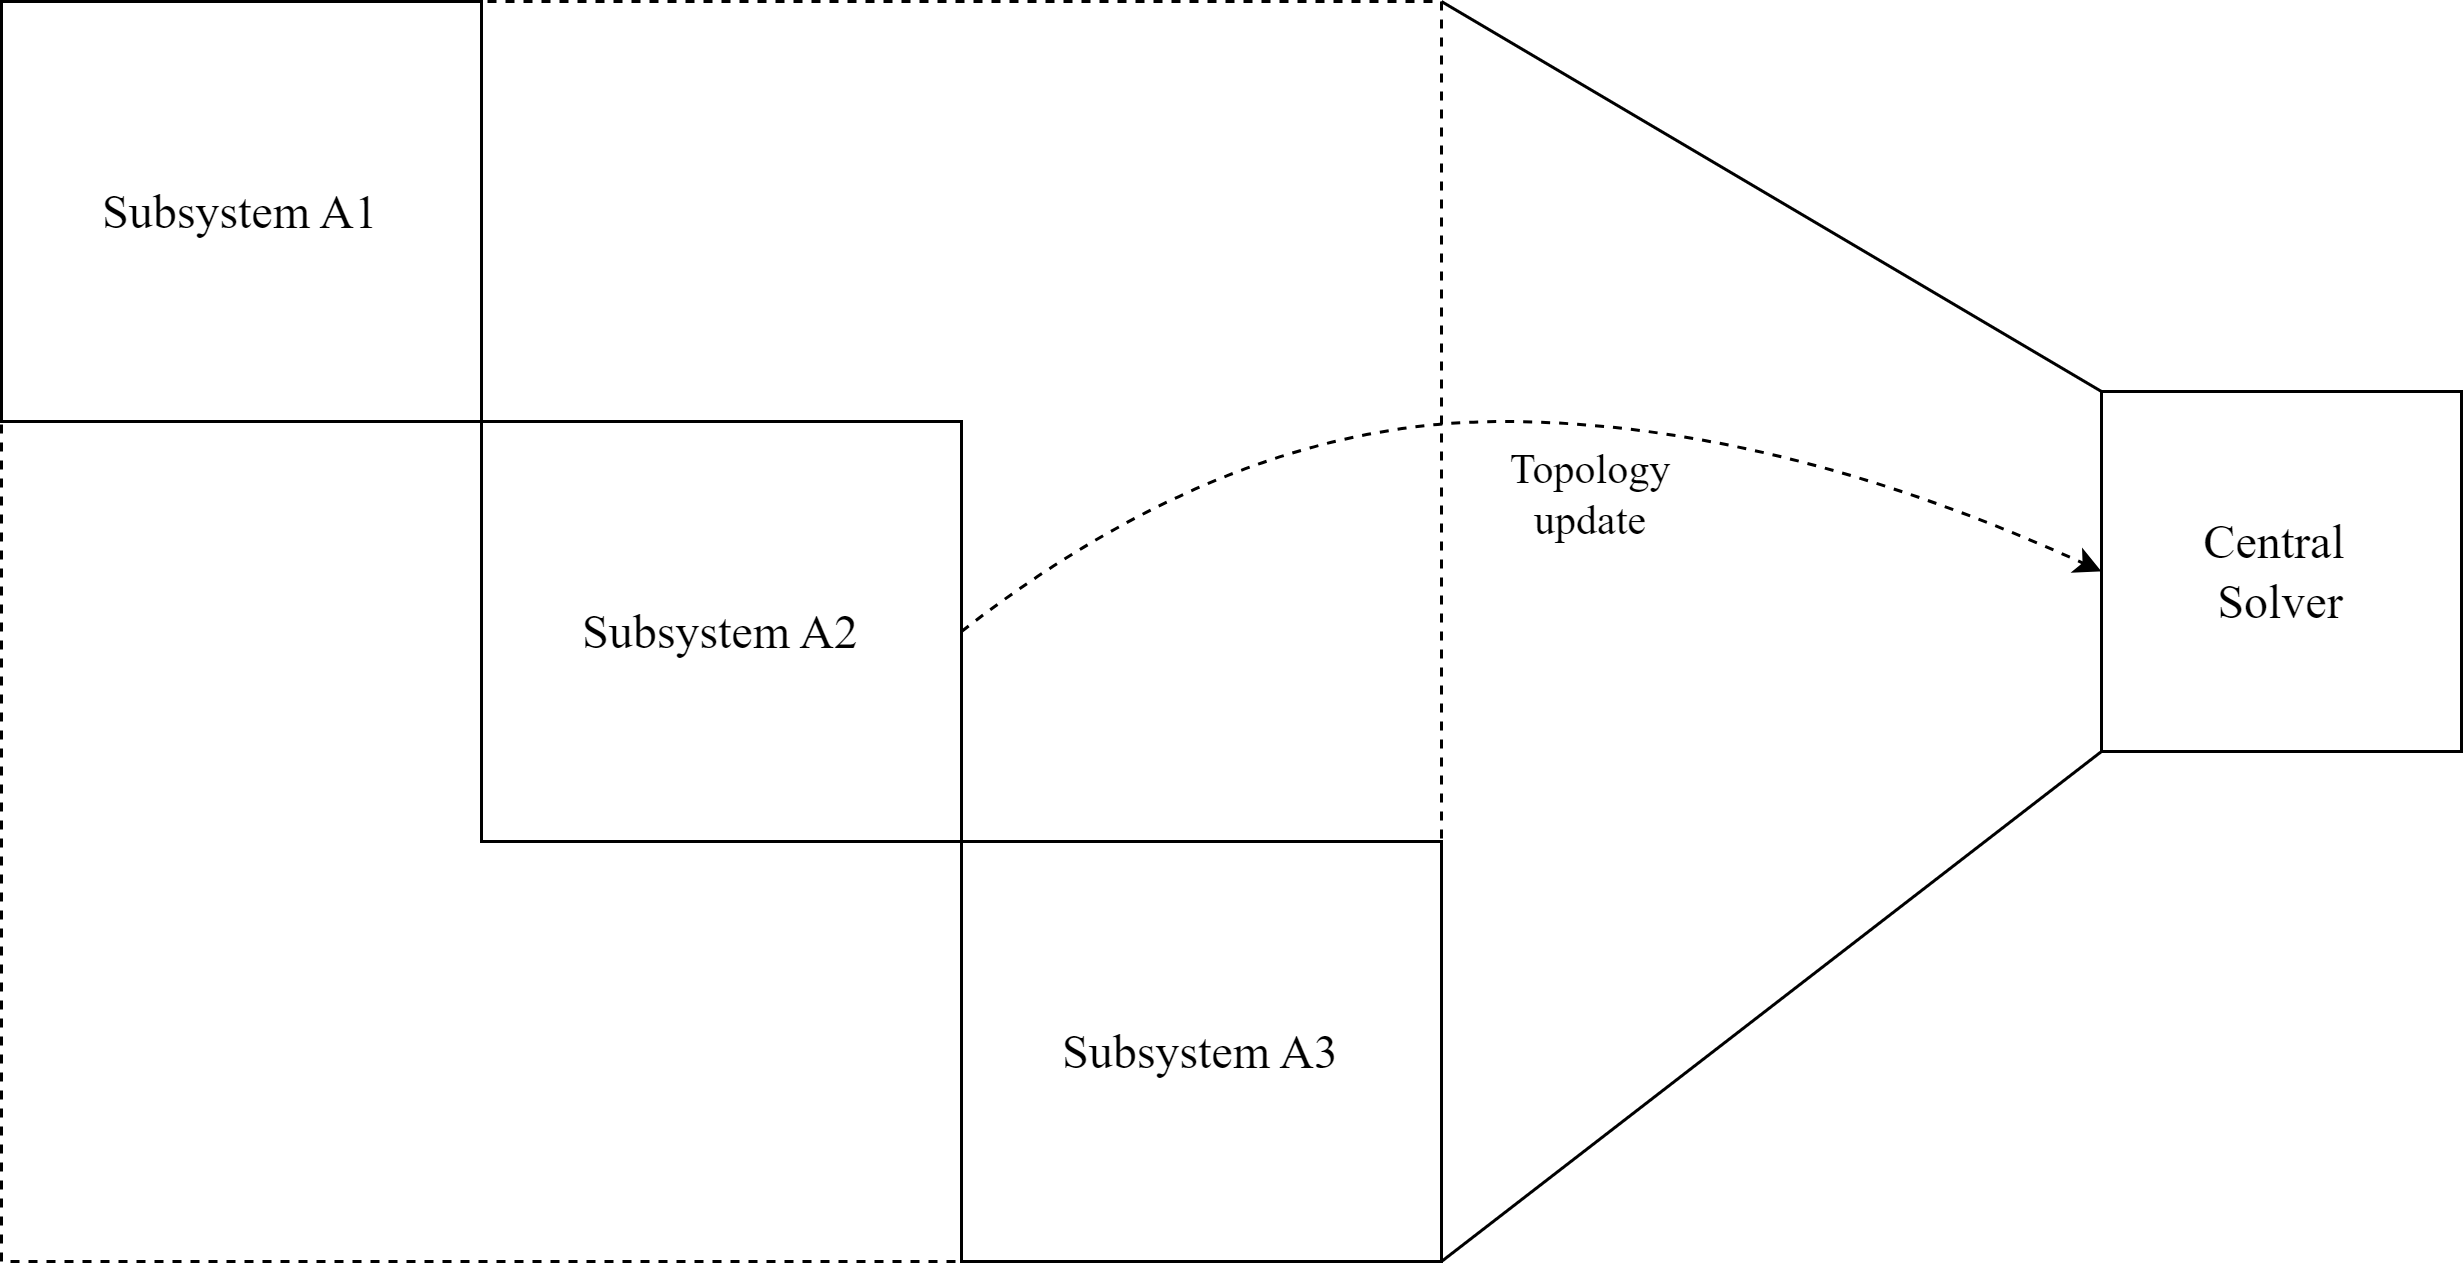
\includegraphics[width = 1\columnwidth]{mate_mc.png}
    \caption{MATE based scheme for multi-core discrete state-space formulation}
    \label{fig:mate_mc}
\end{figure}

To realize such an approach at the hardware level a modern co-simulation concept can be used. A modern co-simulation based approach utilizes the shared memory of computing resources. High-performance shared memory interface can allow multiple processes to directly exchange data with minimal overhead, supported by synchronization mechanisms to ensure consistency at each simulation time step \autocite{Marcus_2021, 8973964}. Simplified scheme of communication, synchronization process, and model interfaces are shown in Figure~\cref{fig:mate_ddm}.

\begin{figure}[htbp]
    \centering
    \includegraphics[width = 1\columnwidth]{mate_ddm.png}
    \caption{Concept of digital twin simulation by shared memory parallelization}
    \label{fig:mate_ddm}
\end{figure}


           % Глава 3
\chapter{Case Study and Results}\label{ch:ch4}

To demonstrate the feasibility of the fundamental functions of the proposed DT-based dynamic mirroring, an appropriate method of power systems studies should be chosen. This can be aided by the use of high-fidelity studies of steady-state and transient conditions in field tests, virtual dynamic simulations, and hardware-in-the-loop  tests. The methods can provide information on the overall impact of DT application on existing power systems \autocite{10202933}. Table \ref{tab:study_methods} compares methods for conducting power system studies: field tests, virtual simulations, and cyber-physical tests.

\begin{table}[htbp]
    \centering
    \caption{Comparison of Study Methods \autocite{10202933}}
    % \begin{tabular}{|c|c|c|c|}
    \begin{tabular}{|>{\centering\arraybackslash}m{2.5cm}|>{\centering\arraybackslash}m{4cm}|>{\centering\arraybackslash}m{4.5cm}|>{\centering\arraybackslash}m{4.5cm}|}
        \hline
        \textbf{Property} & \multicolumn{3}{c|}{\textbf{Studies Methods}} \\ \cline{2-4}
        & \textbf{Field tests} & \textbf{Virtual simulations} & \textbf{Cyber-physical tests} \\ \hline
        Realism & Realistic evaluation of new technologies & May not accurately replicate the behavior of real-world power systems & High, combines real-world behavior with the flexibility of virtual simulations \\ \hline
        Cost & Expensive, require the personnel, setup of equipment & Cost-effective, do not require the use of physical prototypes or testbeds & Expensive, require the integration of physical power systems with computer-based environments \\ \hline
        Time & Time-consuming, require the personnel, setup of equipment & Fast, can be conducted without the need for physical setup & Fast, allow for the simultaneous run of multiple scenarios in a short period of time \\ \hline
        Flexibility & Limited, because conducted with fixed operating conditions & High level, can be conducted with variable operating conditions & High level, allow for the simultaneous run of multiple scenarios in a single test \\ \hline
    \end{tabular}
    \label{tab:study_methods}
\end{table}

In this work, for the DT mirroring study, cyberphysical power system tests, also known as hardware-in-the-loop (HIL) tests are chosen as they involve the integration of physical power systems with computer-based simulations to create a hybrid testing environment that combines the benefits of both field tests and virtual simulations \autocite{7289345}. HIL tests offer a high level of realism as they combine the real-world behavior of physical power systems with the control and flexibility of computer-based simulations. One of the main advantages of HIL tests is their ability to evaluate the performance of new technologies under realistic operating conditions. In contrast to virtual simulations, which are based on computer models that may not accurately replicate the behavior of real-world power systems, HIL tests offer a more accurate evaluation of new technologies by incorporating physical equipment. 

The performance of new developing technologies and equipment can be evaluated under transient or fault conditions. Another advantage of HIL tests is their ability to evaluate the interaction between different components of a power system. In contrast to field tests, which may only evaluate the performance of a single component or subsystem, cyber-physical type can be used to evaluate the performance of multiple components or subsystems simultaneously. This is particularly useful for complex power systems, such as microgrids or distribution systems, as it allows the evaluation of the interaction between different components. In general, cyber-physical power systems tests offer a unique combination of realism, flexibility, and precision for the evaluation of new technologies in power systems. They offer a higher level of realism and the ability to evaluate the interaction between different components of a power system \autocite{7740849}. In this work HIL tests are built based on RTDS and OPAL-RT simulators with data channels interaction, as shown in Figure~\cref{fig:hil_bench}.

\begin{figure}[ht]
    \centering
    \includegraphics[width = 1\columnwidth]{hil_bench.png}
    \caption{Hardware-in-the-loop test bench.}
    \label{fig:hil_bench}
\end{figure}


\section{Description of the Physical grid}\label{sec:ch4/sec1}

For the test case, the simplified microgrid structure with distributed energy resources depicted in Figure~\cref{fig:cs_microgrid} has been chosen. It consists of the feeder 0.4 $kV$ feeder with a nominal frequency of 50 $Hz$, connected to the distribution grid via a 6/0.4 kV power transformer. The microgrid includes three connected DERs throw 4Q power inverters working in grid following mode. In addition, three consumers are connected, represented by a flexible load with active and reactive power set-points. All elements in the grid are connected with transmission lines, which are basically RL elements.

\begin{figure}[ht]
    \centering
    \includegraphics[width = 1\columnwidth]{cs_microgrid.png}
    \caption{Simplified microgrid structure with distributed energy resources.}
    \label{fig:cs_microgrid}
\end{figure}

According to the definition of DT technology in Section \ref{sec:dt_approach}, we must have a physical object with which to test the DT approach. HIL test bench allows us to realize the physical object as real hardware-connected throw amplifier or fully detailed EMT models. The basic parameters of the EMT model follow Table \ref{tab:base_model_param}.  The renewable generation and storage system are in the center of interest of this work and will be further discussed in detail. 


\begin{table}[htbp]
\centering
    \caption{RTDS EMT Model Parameters}
\begin{tblr}{
  hlines,
  vlines,
}
\textbf{Parameter} & \textbf{Quantity} & \textbf{Value} \\
    $T_{s}$ & Main model execution time  & 50 $us$    \\
    % $t_{\delta}$ &  Data exchange delay  & 10 ms \\
    $V_{g}$ & Grid nominal voltage  & 0.4 $kV$    \\
    $V_{g}$ & Grid nominal frequency   & 50 $Hz$   \\
    $P_{n}$ & Load/Generators nominal power   & 100 $kVA$   \\
    $TL_{R}$ &  TL active resistance  & 0.01644 $Ohm/km$ \\
    $TL_{L}$ &  TL reactive resistance  & 0.003048 $Ohm/km$ \\
    % $TL_{R}, TL_{L}$ &  {TL active resistance and\\ reactive resistance}  & {0.01644 $Ohm/km$,\\ 0.003048 $Ohm/km$} \\
\end{tblr}
\label{tab:base_model_param}
\end{table}

\subsection{Photovoltaics}\label{subsec:ch4/sec1/sub1}
Solar generation is presented by EMT blocks from the RTDS software library. The RTDS photovoltaic model consists of an array of solar cells, a mathematical model of which is represented as a current source in parallel with a single diode, as shown in Figure~\cref{fig:pv_model}. 

\begin{figure}[ht]
    \centering
    \includegraphics[width = 0.7\columnwidth]{pv_model.png}
    \caption{Equivalent model of solar cell in RTDS simulator}
    \label{fig:pv_model}
\end{figure}

The parameters of the solar cell are presented in Table \ref{tab:pv_model_param}. The number of modules is selected in such a way as not to exceed the common voltage of 700 $V$ on the DC bus and around 100 $kW$ at the maximum power point. The temperature regime chosen as normal and suggested as a constant of 25 degrees. The solar intensity input follows the profile with setpoints, the form of which is typical for the south of Russia. 

\begin{table}[htbp]
\centering
    \caption{Photovoltaics Module Parameters}
\begin{tblr}{
  hlines,
  vlines,
}
\textbf{Name} & \textbf{Description} & \textbf{Value} \\
    $N_c$ & {Number of series connected cells\\ per string per module} & 40 \\
    $N_{cp}$ & Number of parallel strings of cells & 10 \\
    $V_{ocref}$ & Open circuit voltage & 21.7 $V$\\ 
    $I_{scref}$ & Short circuit current & 3.35 $A$\\
    $V_{mpref}$ & Voltage at Pmax  & 17.4 $V$\\
    $I_{mpref}$ & Current at Pmax  & 3.05 $A$\\
    $E_g$ & {Energy gap: select semiconductor\\ material of solar cell} & {Monocrystalline\\ Silicon} \\
    $J_{tmp}$ & Short circuit current temperature coefficient & 0.065 $\%/^\circ C$\\
    $K_v$ & Open circuit voltage temperature coefficient & -0.56 $\%/^\circ C$\\
    $T_{ref}$ & Reference temperature at standard test conditions & 25 $^\circ C$\\
    $INS_{ref}$ & Initial reference solar intensity & 1000 $W/m^2$ \\
    $R_{so}$ & Open circuit series resistance & 0.5 $Ohm$\\
    $R_{sho}$ & Short circuit shunt resistance & 100 $Ohm$\\
\end{tblr}
\label{tab:pv_model_param}
\end{table}

The solar module is connected to the grid throw IBR with an integrated maximum power point tracking mechanism. IBR involved as three-phase inverter with boost converter in series according the schematic in Figure~\cref{fig:pv_ibr}.
% , following the parameters in Table \ref{tab:pv_ibr_param}. 

\begin{figure}[ht]
    \centering
    \includegraphics[width = 1\columnwidth]{pv_ibr.png}
    \caption{Photovoltaic array module with IBR connection}
    \label{fig:pv_ibr}
\end{figure}

% \begin{table}[h]
% \centering
%     \caption{EMT Model Parameters for PV-to-Grid IBR Interface}
% \begin{tblr}{
%   hlines,
%   vlines,
% }
% {Parameter & Quantity & Value} \\
%     $P_{ibr}$ & IBR nominal power   & 100 kVA   \\
%     $F_{sw}$ & IBR PWM base frequency  & 20 kHz    \\
%     $L_{1}, L_{2}$  & IBR Filter inductance  & {6.2 mH,\\ 4.58 uH}  \\ 
%     $R_{1}, R_{2}$  & IBR Filter resistance  & {19.6 mOhm,\\ 0.14 uOhm}  \\ 
%     $C_{f}$  & IBR Filter capacitance  & 82.89 uF   \\ 
%     $K_{p}^{cc}$ & {IBR Current control\\ proportional gain}  & 9.36   \\
%     $K_{i}^{cc}$ &  IBR Current control integral gain  & 29.4   \\
%     $K_{p}^{pll}$ &  IBR PLL proportional gain  & 5   \\
%     $K_{i}^{pll}$ &  IBR PLL integral gain  & 0,1 
% \end{tblr}
% \label{tab:pv_ibr_param}
% \end{table}

\subsection{Wind turbine}\label{subsec:ch4/sec1/sub2}

The wind turbine model represented by the dynamic model of a Type 4 wind power generator, the scheme of which is depicted in Figure~\cref{fig:wt_scheme}. The standard RTDS model is based on a variable-speed wind turbine with Permanent Magnet Synchronous Machine (PMSM) and connected to an AC grid through a full-scale back-to-back three-level VSC. The time domain modeling of this PMSM model is based on the theory $dq0$. The $dq$ equivalent circuit of the PMSM is shown below in Figure~\cref{fig:pmsm_model}. 

\begin{figure}[ht]
    \centering
    \includegraphics[width = 1\columnwidth]{wt_scheme.png}
    \caption{Schematic block diagram of type 4 wind generation model in RTDS simulator}
    \label{fig:wt_scheme}
\end{figure}
\begin{figure}[ht]
    \centering
    \includegraphics[width = 1\columnwidth]{pmsm_model.png}
    \caption{Equivalent PMSM Model in RTDS simulator}
    \label{fig:pmsm_model}
\end{figure}

The VSC simulated by detailed EMT model with 12 power transistors, which is AC/DC and DC/AC parts in series, firing by PWM plant. The DC/AC part follows the same parameter as for solar IBR from Table \ref{tab:pv_ibr_param}. The output power limited by 100 $kW$ and the reference set point follow the profile characteristic for the south regions of Russia. As models consist of many blocks with complex control systems, the only most sensitive parameters are presented in Table \ref{tab:wt_model_param}. 

\begin{table}[htbp]
\centering
    \caption{RTDS EMT Wind Turbine Model Parameters}
\begin{tblr}{
  hlines,
  vlines,
}
\textbf{Name} & \textbf{Description} & \textbf{Value} \\
    % $V_r$ & {Rated Voltage (L-L RMS)} & 0.690 $kV$ \\
    $P_{n}$ & Rated MVA of the Machine & 0.1 $MVA$ \\
    $X_s$ & Stator Leakage Reactance & 0.1 $pu$\\ 
    $X_{md}$ & D-axis Unsaturated Magnet Reactance & 0.5 $pu$\\
    $X_D$ & D-axis Damper Leakage Reactance  & 2.265 $pu$\\
    $X_{mq}$ & Q-axis Magnetizing Reactance  & 0.2 $pu$\\
    $X_Q$ & Q-axis Damper Leakage Reactance & 2.265 $pu$ \\
    $r_s$ & Stator Resistance & 0.01 $pu$\\
    $r_D$ & D-axis Damper Resistance & 2.0 $pu$\\
    $r_Q$ & Q-axis Damper Resistance & 2.0 $pu$\\
    $V_{dc}$ & Rated DC voltage (pole-pole) & 1.2 $kV$\\
    $R_{dc}$ & DC link R & 0.1 $m\Omega$\\
    $L_{dc}$ & DC link L & 2 $\mu H$\\
    $C_{dc}$ & Aggregated Smoothing capacitor (C/2) & 2000 $mF$\\
    $F_{sw}^{pmsm}$ & Switching Frequency (PMSM-side converter)  & 3 $kHz$\\
    $F_{sw}^{ac}$ & Switching Frequency (Grid-side converter)  & 20 $kHz$
\end{tblr}
\label{tab:wt_model_param}
\end{table}


\subsection{Energy Storage System}\label{subsec:ch4/sec1/sub3}

Dynamic Digital Mirroring applicable for all participant of energy exchange and ESS a powerful example of it, and a vivid example of it is a  VRFBs. The VRFB (5 kW/ 10 kWh) at the Skolkovo Institute of Science and Technology, that shown in Figure~\cref{fig:vrfb_setup},  was elaborated to gather experimental data. The parameters of the system are listed in Table \ref{tab:vrfb_setup_param}.

\begin{figure}[ht]
    \centerfloat{
        \includegraphics[scale=0.8]{vrfb_setup.png}
    }
    \caption{The VRFB (5 kW/ 10 kWh) setup.}\label{fig:vrfb_setup}
\end{figure}

\begin{table}[htbp]
\centering
    \caption{Specification of VRFB Experimental Setup}
\begin{tblr}{
  hlines,
  vlines,
}
\textbf{Name} & \textbf{Description} & \textbf{Value} \\
    $V_{tk}$ & Electrolyte volume held in the storage tanks & 0.045 $m^3$ \\
    $L \times h \times w$ & Electrode's geometrical dimensions & $325 \times 190 \times 3$ $mm$ \\
    $V_{cell}$ & Half-cell's electrolyte content volume & $27 \cdot 10^{-5}$ $m^3$\\ 
    $A_m$ & Membrane area & 0.0848 $m^2$\\
    $N$ & Number of cells in the stack  & 38 \\
    $d_m$ & Membrane thickness,  & $5 \cdot 10^{-5}$ $m$\\
    $c_b$ & Baseline levels of vanadium ions present & 1106 $mol ~m^{-3}$ \\
    $Q$ & Range of flow rates & $[4 ; 10]$ $l ~min^{-1}$\\
    $V_{cut}$ & Cut-off voltages & $[40 ; 65]$ $V$\\
    $SOC_{\Delta}$ & Operating SoC range & $[5 ; 95]$ $\%$\\
    $I_{\Delta}$ & Applied current range & $[0 ; 60]$ $A$\\
    - & Membrane type & AEM\\
    $I_{\Delta}$ & Applied current range & $[0 ; 60]$ $A$\\
\end{tblr}
\label{tab:vrfb_setup_param}
\end{table}

Applying the identification method from Section \ref{subsec:ch3/sec1/sub1} the equivalent overall vanadium concentration $c_b$, the crossover multiplication factor $\gamma$, the formal potential of the cell $U_0^*$, cell resistivity $r_{c e l l}$, the slope $\alpha$ and the growth rate  $\beta$ of the mass transfer coefficient were estimated and presented in Table \ref{tab:vrfb_idtf_param}. 

\begin{table}[htbp]
\centering
    \caption{Identified parameters of VRFB Experimental Setup}
\begin{tblr}{
  hlines,
  vlines,
}
\textbf{Name} & \textbf{Description} & \textbf{Value} \\
    $\gamma$ & Crossover factor & 1.03 $m^3$ \\
    $c_0$ & Equivalent overall  battery concentration & $1.450 \times 10^3$ $mol/m^{3}$ \\
    $ASR$ & Area specific resistance & 2.231 $\Omega cm^2$\\ 
    $U_0^*$ & Formal potential & 1.38 $V$\\
    $\alpha$ & Slope of mass transfer  coefficient  & $1.64 \times 10^{-4}$ \\
    $\beta$ & Growth of mass transfer  coefficient  & 0.4\\
\end{tblr}
\label{tab:vrfb_idtf_param}
\end{table}


% These relates with internal physical and chemical processes that occur during operation, such as the undesired migration of vanadium ions via the membrane, electrode activation, concentration, and ohmic polarizations, as well as capacity deterioration over time because of uneven vanadium concentrations. For identification of the VRFB system parameters we used the approach proposed in our previous work \cite{jrn_bogdanov_2023}.

% The VRFB model presented above involves the identification of six unknown parameters, including the equivalent overall vanadium concentration $c_b$, the crossover multiplication factor $\gamma$, the formal potential of the cell $U_0^*$, cell resistivity $r_{c e l l}$, the slope $\alpha$ and the growth rate  $\beta$ of the mass transfer coefficient:
% \begin{equation}
%     \label{eq:idn}
%     \xi=\left(c_b, \gamma, r_{c e l l}, U_0^*, \alpha, \beta\right)^T .
% \end{equation}

% To be as close as possible to real conditions, the VRFB (5 kW/ 10 kWh) at the Skolkovo Institute of Science and Technology was used with Ponovo amplifier as interface to HIL simulator, as shown in Figure~\cref{fig:vrfb_panovo}. The parameters of the system are listed in Table \ref{tab:vrfb_setup_param}.

% \begin{figure}[htbp]
%     \centering
%     \includegraphics[width = 1\columnwidth]{vrfb_panovo.png}
%     \caption{Equivalent PMSM Model in RTDS simulator}
%     \label{fig:vrfb_panovo}
% \end{figure}

% The ultimate design of the DT for the VRFB state of charge estimator is depicted in Fig.~\ref{fig:vrfb_dt}. By leveraging digital twin technology, this state estimator acquires and interprets signals related to current, temperature, and flowrate, achieving real-time dynamic monitoring of the battery's state, SOC and output stack voltage particularly. 


The system is equipped with industrial-grade sensors such as ambient temperature, open-circuit voltage at stack input, flow rate of positive electrolyte, flow rate of negative electrolyte, output stack voltage and current. Sensor measurements collected by PLC, which are then transmitted to an OPC server via Modbus TCP protocol.

\section{Description of the Digital Twin}\label{sec:ch4/sec2}

The ultimate design of the DT for the VRFB dynamic mirroring is depicted in Figure~\cref{fig:vrfb_dt}. By leveraging digital twin technology, this estimator acquires and interprets signals related to current, temperature, and flowrate, achieving real-time monitoring of the battery's state. This setup provides accurate SOC and output stack voltage, tacking into accoun degradation of battery and crossover effect \autocite{10615087}.

\begin{figure}[htbp]
    \centerfloat{
        \includegraphics[scale=0.9]{vrfb_dt}
    }
    \caption{Flowchart of the DT based SoC estimation.}\label{fig:vrfb_dt}
\end{figure}

To mirror the dynamic picture of the whole feeder, the DT dynamic model must be consisted of the aggregated discrete inverter model working in grid-following mode and receiving power references from measurements devices installed in physical grids in PCC. According to the DT building method described in Chapter \ref{ch:ch3}, the aggregated discrete inverter model can be implemented with connection to the grid network consisting of RL equivalents of transmission lines. At first, the inverter parameters must be obtained for grid-following mode. 

Basically, we can find ourselves in three different situations. All inverter parameters are known from the beginning of the DT building process, and the connected generator represents to us as a white box. This situation is more specific for the transmission grid level which is strongly regulated and all generative equipment is checking for compatibility. For low voltage level, distribution grid, which we assumed to test, the connected equipment is presented by hundreds of suppliers and parameters usually hidden for us. In this case, the connected generator is represented as a black box. 

As a possible way to deal with that is to try to move in gray box section where parameters are partially available. It can be reached by taking into account that information about the maximum power level is usually available. For example, the typical household connection in Russia is limited to 15 $kW$. The renewables from small commercial owners does not exceed hundreds of kW and is also agreed prior to the permit being issued. Another suggestion may be that the usual PWM frequency accepted in industry is 20 or 40 kHz. Thus, the initial parameters for calculating the filter components are as follows.

\begin{table}[htbp]
\centering
    \caption{Initial Electrical Parameters of the Inverter}
\begin{tblr}{
  hlines,
  vlines,
}
\textbf{Name} & \textbf{Description} & \textbf{Value} \\
    $V_{n}$ & Grid voltage & 230 $V$ \\
    $P_{n}$ & Output power of the inverter & 100 $kVA$ \\
    $V_{dc}$ & DC-Link voltage & 700 $V$\\ 
    $F_g$ & Grid frequency & 50 $Hz$\\
    $F_{sw}$ & Switching frequency  & 20 $kHz$ \\
    $PF$ & Power factor  & 1 \\
\end{tblr}
\label{tab:ibr_initial_param}
\end{table}

Following the well-known LCL filter design for grid-connected system \autocite{Kahlane2015LCLFD}, we calculate at the beginning the base impedance and capacitance, respectively: 
\begin{equation}
    \begin{aligned}
        & \mathrm{Z}_{\mathrm{b}}=\mathrm{U}_{\mathrm{n}}^{2} / \mathrm{S}_{\mathrm{n}} = 0.529,\\
        & \mathrm{C}_{\mathrm{b}}=1 / \omega_{\mathrm{n}} \times \mathrm{Z}_{\mathrm{b}} = 0.006.
    \end{aligned}
\end{equation}

Inverter side inductance $L_i$ allows to limit the output current ripple by up to 10\% of the nominal amplitude.
\begin{equation}
    \begin{aligned}
        & \Delta \mathrm{I}_{\mathrm{L}-\max }=0.01 \frac{\mathrm{P}_{\mathrm{n}} \sqrt{2}}{\mathrm{V}_{\mathrm{n}}} = 6.15,\\
        & \mathrm{L}_{\mathrm{inv}}=\frac{\mathrm{U}_{\mathrm{DC}}}{16 \mathrm{F}_{\mathrm{sw}} \Delta \mathrm{I}_{\mathrm{L}-\max }} = 3.56e-04.
    \end{aligned}
\end{equation}

The filter capacity based on the maximal power factor variation acceptable by the grid is 5\% can be calculated as a multiplication of the system base capacitance $C_b$. The grid side inductance $L_g$ can be calculated based on the factor $r = 0.6$, between $L_{inv}$ and $L_g$:
\begin{equation}
    \begin{aligned}
        & C_{f}=0.05 C_{b} = 3e-04,\\
        & L_g = r \times L_{inv} = 2.14e-04.
    \end{aligned}
\end{equation}

The final phase of the design involves managing the filter's resonant frequency. It should be distinct from the grid frequency and at least half of the converter's switching frequency to ensure sufficient attenuation. The resonant frequency for the L-C-L filter is calculated by:
\begin{equation}
    \mathrm{w}_{\mathrm{res}}=\sqrt{\frac{\mathrm{L}_{\mathrm{inv}}+\mathrm{L}_{\mathrm{g}}}{\mathrm{~L}_{\mathrm{inv}} \times \mathrm{L}_{\mathrm{g}} \times \mathrm{C}_{\mathrm{f}}}} = 5e+03.
\end{equation}

In order to reduce oscillations and unstable states of the filter, the damping resistor is required:
\begin{equation}
    \mathrm{R}_{\mathrm{d}}=\frac{1}{3 \omega_{\mathrm{res}} \mathrm{C}_{\mathrm{f}}} = 0.256.
\end{equation}

The next step is to define the current control dynamics by defining the PI parameters based on (\ref{eq:cc_pi}). Suggesting recommended bandwidth of 1500 $rad/s$ for the current controller:
\begin{equation}
    \begin{array}{l}
        k_{p}=(L_{inv}+L_{g}) w_c = 0.854, \\
        k_{i}=\left(R_{inv}+R_{g}\right) w_c = 2.682.
    \end{array}
    \label{eq:cc_pi_num}
\end{equation}

The PLL parameters are not hidden and are usually provided by signal processor developers \autocite{ti_sprabt3a}. Thus, the full set of parameters involved in the dynamic modeling of inverters are summarized in Table \ref{tab:ibr_sum_param}.

\begin{table}[htbp]
\centering
    \caption{Summarized Parameters of Inverter Dynamic Model}
\begin{tblr}{
  hlines,
  vlines,
}
\textbf{Name} & \textbf{Description} & \textbf{Value} \\
    $L_{inv}$ & Inverter side inductance & 356 $\mu H$ \\
    $R_{inv}$ & Inverter side resistance & 1.1 $mOhm$ \\
    $L_{g}$ & Grid side inductance & 214 $\mu H$ \\
    $R_{g}$ & Grid side resistance & 67 $mOhm$ \\
    $C_{f}$ & Filter capacitance & 300 $\mu F$\\ 
    $R_d$ & Filter damping resistance & 256 $mOhm$\\
    $K_p^{cc}$ & Proportional part of current controller& 0.854 \\
    $K_i^{cc}$ & Integral part of current controller& 2.682 \\
    $K_p^{pll}$ & Proportional part of PLL controller& 5.0 \\
    $K_i^{pll}$ & Integral part of PLL controller& 0.1 \\    
\end{tblr}
\label{tab:ibr_sum_param}
\end{table}

Using the average dynamic modeling method with the parameters calculated above, three IBRs connected to transmission lines have been realized in the form of a discrete simulation model. The next step is to connect the model that represents the DT with the physical grid, using data exchange channels, according to the diagram, shown in Figure~\cref{fig:dt_dse}. 

\begin{figure}[htbp]
    \centering
    \includegraphics[width = 1\columnwidth]{dt_dse.png}
    \caption{Diagram of the DT based mirroring of PEDG.}
    \label{fig:dt_dse}
\end{figure}

Dynamic mirroring is achieved within computation devices that include analog/digital communication channels and where the DT real-time modeling is computed. The received three-phase voltage signal measured at the feeder head of the real grid is sent as a reference to the voltage source inside the virtual feeder in the DT model. It creates a reference sinusoidal voltage in the DT model, to which synchronizes all IBRs. The current flow in the virtual feeder is created by the power consumption of the virtual load and the bidirectional power flow of the virtual inverters. These allow real-time monitoring of the three-phase voltage and current sinusoidal signals at any location along the feeder.

\section{Digital Twin Transient Response Following}\label{sec:ch4/sec3}

\textbf{DT for VRFB validation}. To evaluate the DT model's ability to accurately respond to current variations, the power profiles for DC source were prepared and tested. At first, charging and discharging process were made with constant current mode according the profile in Figure~\cref{fig:statprofile_i} to identify the parameters of the battery. Figure~\cref{fig:statprofile_v} shows the voltage transients during power injection and consumption.

The Nernst equation's characterization of the open circuit voltage (OCV) is the most popular signal used in designing SOC observers of industrial scale batteries.  The Nernst law gives rise to the following equation, which can be employed to determine the SOC \cite{jrn_trovo_2020}:
\begin{equation}
    \label{eq:soc_ocv}
    S O C=\frac{e^{\left(O C V-U_0\right) n F / 2 R T}}{1+e^{\left(O C V-U_0\right) n F / 2 R T}}100,
\end{equation}
where $U_0 = 1.37 V$ is the formal potential for vanadium couples $(T = 298 K)$. 

Thus, there are two different methods that can be used for estimation of instant battery state of charge. The first approach is based on application of inlet OCV data following the indirect estimation of SOC with application of Nernst equation. The  second method is based on the direct calculation of the SOC from the concentrations of vanadium ions. Since the proposed DT methodology demonstrates the capacity to estimate the internal states by factoring in the vanadium species concentration, it enables us to calculate the SOC based on \cref{eq:soc_dt} and inlet OCV based on \cref{eq:ocv_dt}. 

\begin{equation}
    \label{eq:ocv_dt}
    OCV=U_0^*+\frac{R T}{F} \ln \left[\left(\frac{c_5}{c_4}\right)\left(\frac{c_2}{c_3}\right)\right].
\end{equation}

To show the high accuracy of this main indicators, an experiment was performed with multi-step constant current profile presented on Figure~\cref{fig:dynprofile_i}. The comparison of the inlet OCV curves and computed SOC based on different sources is shown in Figure~\cref{fig:dynprofile_ocv} and Figure~\cref{fig:dynprofile_soc} respectively. An additional feature of digital twin application is voltage monitoring, the result of which is shown in Figure~\cref{fig:dynprofile_v}.   

As can be seen from the plots, the battery behavior obtained by application of DT approach follows the VRFB test bench inlet OCV and stack output voltage measurements with high accuracy. It is allows to observe the SOC in real-time maintaining a maximum error below 3 \%.  

Notably, such accurate results can be achieved without the need for additional measurements, utilizing only flow rate, ambient temperature, and stack output current. These findings suggest the application of DT for online state estimation and filtering of corrupted data from sensors.

\begin{figure}[ht]
    \centerfloat{
        \includegraphics[scale=0.25]{statprofile_i}
    }
    \caption{Static current profile.}\label{fig:statprofile_i}
\end{figure}
\begin{figure}[ht]
    \centerfloat{
        \includegraphics[scale=0.25]{statprofile_v}
    }
    \caption{Voltage response to static current profile.}\label{fig:statprofile_v}
\end{figure}
\begin{figure}[ht]
    \centerfloat{
        \includegraphics[scale=0.23]{dynprofile_i}
    }
    \caption{Multi-step constant current current profile.}\label{fig:dynprofile_i}
\end{figure}
\begin{figure}[ht]
    \centerfloat{
        \includegraphics[scale=0.25]{dynprofile_ocv}
    }
    \caption{Inlet OCV response to multi-step constant current profile.}\label{fig:dynprofile_ocv}
\end{figure}
\begin{figure}[ht]
    \centerfloat{
        \includegraphics[scale=0.5]{dynprofile_soc2}
    }
    \caption{SoC change during multi-step constant current profile.}\label{fig:dynprofile_soc2}
\end{figure}
\begin{figure}[ht]
    \centerfloat{
        \includegraphics[scale=0.5]{dynprofile_v}
    }
    \caption{Voltage change during multi-step constant current profile.}\label{fig:dynprofile_v}
\end{figure}

\textbf{DT for PEDG validation}. To validate the described approach, the physical grid and digital twin were realized on the basis of the proved HIL approach according to the physical asset structure, shown in Figure~\cref{fig:rt_test_bench}. DT is implemented as real-time model within a separate computational device. For the lab application, we have used a real-time simulator (OPAL-RT 5600), but it can be implemented on any digital signal processor or edge devices. To accurately reflect the voltage dynamics of the physical grid, the DT leverages analog-to-digital boards within the OPAL-RT system to receive analog signals from the "real" microgrid, which is emulated by the RTDS simulator.

\begin{figure}[htbp]
    \centering
    \includegraphics[width = 1\columnwidth]{test_bench.png}
    \caption{Hardware-in-the-loop test bench system for DT based dynamic mirroring.}
    \label{fig:rt_test_bench}
\end{figure}

For enhanced monitoring, protection and control, synchronized wave-formed data is preferred \autocite{Xu_Huang_Xie_Li_2022}. However, this can result in an overload of the data transmission system. Consequently, an integrated measurement system has been implemented in which the three-phase sinusoidal signal $V_{abc}$ is measured at the PCC, and $P$ and $Q$ are obtained at each POC of electricity sources, loads or prosumers. The values $P$ and $Q$ are received from the remote terminal units (RTU) by the IEC 60870-5-104 protocol and collected by OPC server. Integrating these measurement datasets within the precise DT model enables the observation of synchronized wave-formed data for voltages and currents across the entire feeder at any given point. In the same time, the usage fast analog measurements from only one point allow to avoid computational and informational complexity within scaling of the grid.

To validate the precision of the DT estimating dynamic states, the response to variations in voltage and frequency due to changes in power flow or frequency deviation of the grid were examined. At the head of the feeder, the system starts in a balanced condition where both the frequency and voltage are considered at their nominal values. 

At 10 seconds, the voltage at the POC of the loads $1$ and $3$ deviates from its nominal level due to changes in power injection and consumption according power curve in Figure~\cref{fig:p_response}. Figure~\cref{fig:v_response} illustrates the voltage transients occurring during power flow load changes at PCC. Figure~\cref{fig:f_response} illustrates the frequency deviations measured in load $1$ caused by a change in the frequency of the external grid generator. The droop coefficient for the external grid generator set is relatively small to be sensitive to load variation within the microgrid. The voltage and frequency response in the digital twin estimator shows good accuracy with small difference that is considered negligible and has no significant impact on overall performance or system operation.

\begin{figure}[htbp]
    \centering
    \includegraphics[width = 0.8\columnwidth]{p_5.png}
    \caption{Power transient at the point at the point of common coupling.}
    \label{fig:p_response}
\end{figure}
\begin{figure}[htbp]
    \centering
    \includegraphics[width = 0.8\columnwidth]{v_7.png}
    \caption{Voltage transient response of loads 1 and 3 at point of connection.}
    \label{fig:v_response}
\end{figure}
\begin{figure}[htbp]
    \centering
    \includegraphics[width = 0.8\columnwidth]{f_6.png}
    \caption{Frequency transient response of load 1 at point of connection.}
    \label{fig:f_response}
\end{figure}

\section{Impact of parameter deviations}\label{sec:ch4/sec4}
One critical aspect that often requires thorough investigation is the sensitivity of digital twins to variations in the model parameters. In practical scenarios, the parameters of microgrid participants can deviate from their expected values due to a number of factors, including environmental conditions, operational changes, and unforeseen contingencies. Such discrepancies can lead to significant deviations between the digital twin's predictions and the actual performance of the microgrid. However, through continuous monitoring and analysis of real-time data, the digital twin can detect when there is a considerable difference between the model and reality. Leveraging its set of measurements and advanced analytics, the DT can autonomously perform corrective actions, such as triggering alarms, adjusting parameters to better align with observed conditions, and notifying users of potential issues. 

The greatest impact can be made by power inverters as it has complex dynamics and obviously time delays that can arise due to various reasons, such as control system latency, communication lags, or even physical distance between components. In addition, factors such as aging and manufacturing variability can lead to degradation and a variety of components, such as filter inductance quality. Environmental conditions may necessitate tuning the operational mode and adjusting PI controllers in PLL and the current control loop in the physical device, causing deviations from the DT model.

In this study, we assessed the sensitivity of the DT due to variations in parameters affecting the inverter dynamics between the physical asset and the DT model, specifically the PI controller in the PLL, the PI controller of the current control loop, and the filter inductance. The inverter output voltage at the POC was compared between the DT and the real grid model using a fixed data transfer rate of 10 $ms$. The error was defined as:

\begin{equation}
     \xi(V_{poc}^{inv}) = Y_{DT}(P) - Y_{MG},
\end{equation}
where $P = P_n + \delta P$ represents the actual parameter values with deviations. $P_n$ is the subset of parameters affecting inverter dynamics and communication time delay, including $K_p^{pll}, K_i^{pll}$ - proportional and integral part of the PLL's PI controller, $K_p^{cc}, K_i^{cc}$ - proportional and integral part of the current control loop's PI controller, $L_f$ - filter inductance, $\delta\tau$ - communication delay. 

Our findings in Figure~\cref{fig:s_all} indicate that deviations with 40\% from the nominal in control parameters ($K_i^{cc}, K_p^{pll}, K_i^{pll}$) and output filter ($L_f$) do not significantly affect the error. Inaccuracy in estimating the voltage level in the PCC after a load step do not exceed 200 $mV$. Unlike the current control proportional gain ($K_p^{cc}$), the deviation of which, according Figure~\cref{fig:s_cc},  result in greater errors in the voltage level, potentially reaching nearly 1 $V$. These findings underscore the critical importance of precise tuning in the current control loop to maintain the accuracy of the state estimation.

\begin{figure}[htbp]
    \centering
    \includegraphics[width = 0.8\columnwidth]{all2.png}
    \caption{Voltage error deviation affected by main controller dynamics parameters inequality.}
    \label{fig:s_all}
\end{figure}
\begin{figure}[htbp]
    \centering
    \includegraphics[width = 0.8\columnwidth]{cc_kp4.png}
    \caption{Voltage error deviation affected by proportional part of current control loop parameter inequality.}
    % $K_p^{cc}$ 
    \label{fig:s_cc}
\end{figure}
\begin{figure}[htbp]
    \centering
    \includegraphics[width = 0.8\columnwidth]{meas_delay3.png}
    \caption{Voltage error deviation affected by measurement data transfer delay.}
    \label{fig:s_md}
\end{figure}
\begin{figure}[htbp]
    \centering
    \includegraphics[width = 0.8\columnwidth]{phi2.png}
    \caption{Phase error deviation affected by main controller dynamics parameters inequality.}
    \label{fig:phi}
\end{figure}

Furthermore, the study reveals that hardware configurations and data handling practices significantly influence voltage stability. As shown in Figure~\cref{fig:s_md}, measurement delays, ranging from 50 to 200 $ms$, induce substantial voltage deviation errors of up to ±7 $V$ and setting time up to 0.1 $s$, highlighting the system's extreme sensitivity to data transfer rates. These results emphasize the necessity of minimizing measurement delays up to 10 ms.

The phase match also makes a significant contribution to the accuracy in DSE. From Figure~\cref{fig:phi} it is clear that the greatest impact comes from the data transfer delay and the PLL control loop, causing a deviation of about 0.3 degrees. With an apparent small deviation value, it can lead to an unacceptable operating point of a digital twin. The transmission system yields the power flow equations in its linear approximation (which is rather accurate for distribution grids) \autocite{machowski2020power}: 
\begin{equation}
    P_G = \frac{V_1 V_2}{X_L} \xi(\delta)
    \label{placeholder}
\end{equation}
where $P_G$ represents the power from the IBR. $V_1, V_2$ suggested as voltages directly after the IBR connection and after the transmission line. $X_L$ is reactive resistance of the transmission line. $\xi(\delta)$ represent an error between DT angle and real grid. Substituting 320 $V$ voltage level and 25 $m$ transmission line length within inductance equal to 0.0762 $H/km$ it can be obtained that within 0.3 degrees error the power mismatch will reach about 1 $kW$. This is 1$\%$ from the power level in the feeder head, but only if we take into account only one energy source. In case of hundreds of devices, this can lead to unacceptable inaccuracy of DT based state estimator.

\section{Anomaly Detection Validation}\label{sec:ch4/sec5}
To validate threat detection based on the collaborative work of DT and ML methods, the hardware-in-the-loop technique is utilized with a Man-in-the-middle (MITM) attack. The real microgrid structure is utilized as a detailed electromagnetic transient model within a real-time simulator (RTDS) representing consumers, solar generation, wind generation, and ESS with the appropriate power electronics interface. To reproduce real power flow, logged generation and consuming profiles are used in time as referenced values for power inverters and loads.  DT is represented by an average real-time model implemented in a separate real-time machine OPAL-RT 5600. To accurately reflect the state of the real grid, DT leverages sinusoidal analog voltages at the point of common coupling in the head of the feeder along with digital measurements transmitted from IED by IEC 60870-5-104 protocol. The measured power values received act as reference points for the loads and power inverters in the DT. This configuration guarantees that the overall DT model accurately represents the real-time condition of the physical asset simulated by the RTDS simulator. Figure~\cref{fig:mitm_bench} depicts this detailed test bench configuration.

\begin{figure}[ht]
    \centerfloat{
        \includegraphics[scale=0.7]{mitm_bench}
    }
    \caption{Test bench system for anomalies detection.}\label{fig:mitm_bench}
\end{figure}

\textbf{Dataset Description}. The datasets utilized in this study comprise time-series measurements collected from a power system and DT under both normal operating conditions and simulated attack scenarios. The data include various electrical parameters, such as:
\begin{itemize}
    \item Power Outputs: Photovoltaic active and reactive power ($P_{pv}, Q_{pv}$), battery active and reactive power ($P_{batt}, Q_{batt}$), wind active and reactive power ($P_{w}, Q_{w}$) and consumer active and reactive powers ($P_{n}, Q_{n}$) – all received from IEDs.
    \item Voltage Levels: Voltage virtual measurements estimation from DT at different nodes within the whole feeder ($V_{1}$ to $V_{6}$).
    \item Frequency virtual measurements estimation from DT at different nodes within the whole feeder ($F_{1}$ to $F_{6}$).
    \item Time Stamps: Temporal markers indicating the time of each measurement.
\end{itemize}

\textbf{ML Setup}. All experiments were conducted under the following conditions. For Random Forest Classifier we set the number of estimators to 100, the maximum depth to 10, the minimum samples split to 10, and the minimum samples leaf to 5. For LSTM Neural Network, we used 32 and 64 hidden Units. The learning rate is adjusted between 0.0001 and 0.001 with a number of epochs between 50 and 150 based on convergence observations. The batch size is selected to optimize training efficiency and convergence stability. A kfold cross-validation was performed with to estimate the model’s generalization capability and to validate its stability across different subsets of data. We applied methods such as dropout and weight decay to prevent overfitting in the neural network. We implemented early stopping based on validation loss to prevent overfitting by halting training when no improvement was observed.

\textbf{Performance Metrics}. To evaluate and compare the models, several performances metrics were employed:
\begin{enumerate}
    \item Accuracy: The ratio of accurately predicted instances to the total number of instances assessed:
    \begin{equation}
        \text { Accuracy }=\frac{T P+T N}{T P+T N+F P+F N},
    \end{equation}
    where $TP$, $TN$, $FP$, and $FN$ represent true positives, true negatives, false positives, and false negatives, respectively.
    \item Precision: The fraction of TPs relative to the total of TPs and FPs, representing the accuracy of positive classifications:
    \begin{equation}
        \text { Precision }=\frac{T P}{T P+F P}.
    \end{equation}
    \item Recall: The proportion of TPs compared to the total of TPs and FNs:
    \begin{equation}
        \text { Recall }=\frac{T P}{T P+F N}.
    \end{equation}
    \item F1-Score: The harmonic mean of precision and recall:
    \begin{equation}
        F 1-\text { Score }=2 \times \frac{\text { Precision } \times \text { Recall }}{\text { Precision }+ \text { Recall }} .
    \end{equation}
    \item Confusion Matrix:A matrix that provides a detailed breakdown of correct and incorrect classifications, allowing for the analysis of the types of errors made by the model.
\end{enumerate}

\textbf{Threat Detection Results}. The performance of both the Random Forest and LSTM models was evaluated under two scenarios: using only data from measurement devices and utilizing the DT-enhanced data. The results of these evaluations are presented in Table \ref{tab:performance_metrics}.

% Requires: \usepackage{multirow}
\begin{table}[h]
    \centering
    \caption{ML Performance Metrics}
    \begin{tabular}{|c|c|c|c|c|}
        \hline
        % \multicolumn{2}{|c|}{TABLE I. ML PERFORMANCE METRICS} \\ \hline
        \multirow{2}{*}{Method} & \multicolumn{4}{c|}{Performance Metrics Without DT} \\ \cline{2-5}
         & Accuracy & Precision & Recall & F1-Score \\ \hline
        Random Forest & 0.7434 & 0.73 & 0.77 & 0.75 \\ \hline
        LSTM & 0.8688 & 0.8325 & 0.8183 & 0.8254 \\ \hline
        \multirow{2}{*}{Method} & \multicolumn{4}{c|}{Performance Metrics With DT} \\ \cline{2-5}
         & Accuracy & Precision & Recall & F1-Score \\ \hline
        Random Forest & 0.8692 & 0.7380 & 0.8748 & 0.8006 \\ \hline
        LSTM & 0.9159 & 0.9417 & 0.8669 & 0.9028 \\ \hline
    \end{tabular}
    
    \label{tab:performance_metrics}
\end{table}

The evaluation of threat detection performance revealed that integrating DT-enhanced data significantly improved the accuracy and overall metrics for both Random Forest and LSTM models.

\section{Computational requirements}\label{sec:ch4/sec6}

To be compatible for real-time execution on both real-time machines and edge devices, the DT is realized as a discrete type Matlab Simulink model with 20 us sampling time. The model is characterized by its state variables, inputs and outputs. As the complexity of the microgrid model increases with the number of loads and IBRs connected to the feeder, the computational time also increases, as shown in Table \ref{tab:comp_req}. A test was carried out for non real-time condition on a working station with one core of Intel i5-1135G7 CPU @ 2.4 GHz processor and 32 GB memory. Notice that the execution time grows significantly fast as the number of states increases, showing a power increase with the power of 1.6 approximately. By extrapolating this relationship to a scenario with 100 devices, we can estimate the execution time to be approximately 220 ms. In industrial scenarios with a substantial number of IBRs, the calculation speed must be significantly increased by utilizing multi-core processing and implementing distributed computation.

\begin{table}[htbp]
\caption{Model Execution Time Characteristic}
\label{tab:comp_req}
\centering
\begin{tblr}{
  hlines,
  vlines,
}
Case  & Loads & IBRs & States & Inputs & Outputs & {Execution Time, ms}          \\
1               & 1     & 1    & 19     & 22     & 46      & 0.14                  \\
2               & 2     & 2    & 37     & 38     & 83      & 0.28                  \\
3               & 3     & 3    & 55     & 54     & 120     & 0.45                  \\
4               & 5     & 5    & 91     & 86     & 194     & 1.1                   \\
5               & 10    & 10   & 181    & 166    & 379     & 3.4                   \\
6               & 20    & 20   & 361    & 326    & 749     & 10                   \\
\end{tblr}
\end{table}

Talking about hard real-time execution, such machines as OPAL-RT allows to run on 1 core the case 5 from  Table \ref{tab:comp_req} with 10 kHz frequency. The extension of the number of devices requires to add additional cores and partitioning of the model in analogy with the MATE concept. The best performance can be reached on the basis of System-On-Chips (SoC) solutions which combines multiple CPU cores with an FPGA. This architecture based on MATE approach described in section \ref{sec:dt_method} allows circuit models to be partitioned and computed in parallel on the CPU cores and the FPGA \autocite{ppmpower_rtbox_compare}. Multiple SoC chips, connected via multi-gigabit optical links, can form a scalable real-time simulation cluster. This enables distributed synchronous computation of large circuit models, such as PEDGs.           % Глава 4
\chapter*{Conclusion}                       % Заголовок
\addcontentsline{toc}{chapter}{Conclusion}  % Добавляем его в оглавление

%% Согласно ГОСТ Р 7.0.11-2011:
%% 5.3.3 В заключении диссертации излагают итоги выполненного исследования, рекомендации, перспективы дальнейшей разработки темы.
%% 9.2.3 В заключении автореферата диссертации излагают итоги данного исследования, рекомендации и перспективы дальнейшей разработки темы.
%% Поэтому имеет смысл сделать эту часть общей и загрузить из одного файла в автореферат и в диссертацию:

Основные результаты работы заключаются в следующем.
\input{common/concl}
И какая-нибудь заключающая фраза.

Последний параграф может включать благодарности.  В заключение автор
выражает благодарность и большую признательность научному руководителю
Иванову~И.\,И. за поддержку, помощь, обсуждение результатов и~научное
руководство. Также автор благодарит Сидорова~А.\,А. и~Петрова~Б.\,Б.
за помощь в~работе с~образцами, Рабиновича~В.\,В. за предоставленные
образцы и~обсуждение результатов, Занудятину~Г.\,Г. и авторов шаблона
*Russian-Phd-LaTeX-Dissertation-Template* за~помощь в оформлении
диссертации. Автор также благодарит много разных людей
и~всех, кто сделал настоящую работу автора возможной.
      % Заключение
\include{Dissertation/acronyms}        % Список сокращений и условных обозначений
% \include{Dissertation/dictionary}      % Словарь терминов
\include{Dissertation/references}      % Список литературы
\include{Dissertation/lists}           % Списки таблиц и изображений (иллюстративный материал)

\setcounter{totalchapter}{\value{chapter}} % Подсчёт количества глав

%%% Настройки для приложений
\appendix
% Оформление заголовков приложений ближе к ГОСТ:
\setlength{\midchapskip}{20pt}
\renewcommand*{\afterchapternum}{\par\nobreak\vskip \midchapskip}
\renewcommand\thechapter{\Asbuk{chapter}} % Чтобы приложения русскими буквами нумеровались

% \chapter{Примеры вставки листингов программного кода}\label{app:A}

% Для крупных листингов есть два способа. Первый красивый, но в нём могут быть
% проблемы с поддержкой кириллицы (у вас может встречаться в~комментариях
% и~печатаемых сообщениях), он представлен на листинге~\cref{lst:hwbeauty}.
% \begin{ListingEnv}[!h]% настройки floating аналогичны окружению figure
%     \captiondelim{ } % разделитель идентификатора с номером от наименования
%     \caption{Программа ,,Hello, world`` на \protect\cpp}\label{lst:hwbeauty}
%     % окружение учитывает пробелы и табуляции и применяет их в сответсвии с настройками
%     \begin{lstlisting}[language={[ISO]C++}]
% 	#include <iostream>
% 	using namespace std;

% 	int main() //кириллица в комментариях при xelatex и lualatex имеет проблемы с пробелами
% 	{
% 		cout << "Hello, world" << endl; //latin letters in commentaries
% 		system("pause");
% 		return 0;
% 	}
%     \end{lstlisting}
% \end{ListingEnv}%
% Второй не~такой красивый, но без ограничений (см.~листинг~\cref{lst:hwplain}).
% \begin{ListingEnv}[!h]
%     \captiondelim{ } % разделитель идентификатора с номером от наименования
%     \caption{Программа ,,Hello, world`` без подсветки}\label{lst:hwplain}
%     \begin{Verb}

%         #include <iostream>
%         using namespace std;

%         int main() //кириллица в комментариях
%         {
%             cout << "Привет, мир" << endl;
%         }
%     \end{Verb}
% \end{ListingEnv}

% Можно использовать первый для вставки небольших фрагментов
% внутри текста, а второй для вставки полного
% кода в приложении, если таковое имеется.

% Если нужно вставить совсем короткий пример кода (одна или две строки),
% то~выделение  линейками и нумерация может смотреться чересчур громоздко.
% В таких случаях можно использовать окружения \texttt{lstlisting} или
% \texttt{Verb} без \texttt{ListingEnv}. Приведём такой пример
% с указанием языка программирования, отличного от~заданного по умолчанию:
% \begin{lstlisting}[language=Haskell]
% fibs = 0 : 1 : zipWith (+) fibs (tail fibs)
% \end{lstlisting}
% Такое решение "--- со вставкой нумерованных листингов покрупнее
% и~вставок без выделения для маленьких фрагментов "--- выбрано,
% например, в~книге Эндрю Таненбаума и Тодда Остина по архитектуре
% компьютера.

% Наконец, для оформления идентификаторов внутри строк
% (функция \lstinline{main} и~тому подобное) используется
% \texttt{lstinline} или, самое простое, моноширинный текст
% (\texttt{\textbackslash texttt}).

% Пример~\cref{lst:internal3}, иллюстрирующий подключение переопределённого
% языка. Может быть полезным, если подсветка кода работает криво. Без
% дополнительного окружения, с подписью и ссылкой, реализованной встроенным
% средством.
% \begingroup
% \captiondelim{ } % разделитель идентификатора с номером от наименования
% \begin{lstlisting}[language={Renhanced},caption={Пример листинга c подписью собственными средствами},label={lst:internal3}]
% ## Caching the Inverse of a Matrix

% ## Matrix inversion is usually a costly computation and there may be some
% ## benefit to caching the inverse of a matrix rather than compute it repeatedly
% ## This is a pair of functions that cache the inverse of a matrix.

% ## makeCacheMatrix creates a special "matrix" object that can cache its inverse

% makeCacheMatrix <- function(x = matrix()) {#кириллица в комментариях при xelatex и lualatex имеет проблемы с пробелами
%     i <- NULL
%     set <- function(y) {
%         x <<- y
%         i <<- NULL
%     }
%     get <- function() x
%     setSolved <- function(solve) i <<- solve
%     getSolved <- function() i
%     list(set = set, get = get,
%     setSolved = setSolved,
%     getSolved = getSolved)

% }


% ## cacheSolve computes the inverse of the special "matrix" returned by
% ## makeCacheMatrix above. If the inverse has already been calculated (and the
% ## matrix has not changed), then the cachesolve should retrieve the inverse from
% ## the cache.

% cacheSolve <- function(x, ...) {
%     ## Return a matrix that is the inverse of 'x'
%     i <- x$getSolved()
%     if(!is.null(i)) {
%         message("getting cached data")
%         return(i)
%     }
%     data <- x$get()
%     i <- solve(data, ...)
%     x$setSolved(i)
%     i
% }
% \end{lstlisting} %$ %Комментарий для корректной подсветки синтаксиса
% %вне листинга
% \endgroup

% Листинг~\cref{lst:external1} подгружается из внешнего файла. Приходится
% загружать без окружения дополнительного. Иначе по страницам не переносится.
% \begingroup
% \captiondelim{ } % разделитель идентификатора с номером от наименования
% \lstinputlisting[lastline=78,language={R},caption={Листинг из внешнего файла},label={lst:external1}]{listings/run_analysis.R}
% \endgroup

% \chapter{Очень длинное название второго приложения, в~котором продемонстрирована работа с~длинными таблицами}\label{app:B}

% \section{Подраздел приложения}\label{app:B1}
% Вот размещается длинная таблица:
% \makeatletter
% \@ifpackagelater{longtable}{2024/07/04} % hotfix of bug fixed in https://github.com/latex3/latex2e/commit/7c96b6b90a730278903e71a482d88479789a89a3
% {% Если много longtable* используется и новый latex, то три строки ниже правильней в главную преамбулу унести
% \renewenvironment{longtable*}
%   {\renewcommand\LTcaptype{}\longtable}
%   {\endlongtable}
% }
% {\@ifpackagelater{longtable}{2024/04/26}
%     {\addtocounter{table}{-1}}
%     {}
% }
% \makeatother
% \fontsize{10pt}{10pt}\selectfont
% \begin{longtable*}[c]{|l|c|l|l|} %longtable* появляется из пакета ltcaption и даёт ненумерованную таблицу
%     \hline
%     Параметр & Умолч. & Тип & Описание               \\ \hline
%     \endfirsthead   \hline
%     \multicolumn{4}{|c|}{\small\slshape (продолжение)}        \\ \hline
%     Параметр & Умолч. & Тип & Описание               \\ \hline
%     \endhead        \hline
%     \multicolumn{4}{|r|}{\small\slshape продолжение следует}  \\ \hline
%     \endfoot        \hline
%     \endlastfoot
%     \multicolumn{4}{|l|}{\&INP}        \\ \hline
%     kick & 1 & int & 0: инициализация без шума (\(p_s = const\)) \\
%     &   &     & 1: генерация белого шума                  \\
%     &   &     & 2: генерация белого шума симметрично относительно \\
%     & & & экватора    \\
%     mars & 0 & int & 1: инициализация модели для планеты Марс     \\
%     kick & 1 & int & 0: инициализация без шума (\(p_s = const\)) \\
%     &   &     & 1: генерация белого шума                  \\
%     &   &     & 2: генерация белого шума симметрично относительно \\
%     & & & экватора    \\
%     mars & 0 & int & 1: инициализация модели для планеты Марс     \\
%     kick & 1 & int & 0: инициализация без шума (\(p_s = const\)) \\
%     &   &     & 1: генерация белого шума                  \\
%     &   &     & 2: генерация белого шума симметрично относительно \\
%     & & & экватора    \\
%     mars & 0 & int & 1: инициализация модели для планеты Марс     \\
%     kick & 1 & int & 0: инициализация без шума (\(p_s = const\)) \\
%     &   &     & 1: генерация белого шума                  \\
%     &   &     & 2: генерация белого шума симметрично относительно \\
%     & & & экватора    \\
%     mars & 0 & int & 1: инициализация модели для планеты Марс     \\
%     kick & 1 & int & 0: инициализация без шума (\(p_s = const\)) \\
%     &   &     & 1: генерация белого шума                  \\
%     &   &     & 2: генерация белого шума симметрично относительно \\
%     & & & экватора    \\
%     mars & 0 & int & 1: инициализация модели для планеты Марс     \\
%     kick & 1 & int & 0: инициализация без шума (\(p_s = const\)) \\
%     &   &     & 1: генерация белого шума                  \\
%     &   &     & 2: генерация белого шума симметрично относительно \\
%     & & & экватора    \\
%     mars & 0 & int & 1: инициализация модели для планеты Марс     \\
%     kick & 1 & int & 0: инициализация без шума (\(p_s = const\)) \\
%     &   &     & 1: генерация белого шума                  \\
%     &   &     & 2: генерация белого шума симметрично относительно \\
%     & & & экватора    \\
%     mars & 0 & int & 1: инициализация модели для планеты Марс     \\
%     kick & 1 & int & 0: инициализация без шума (\(p_s = const\)) \\
%     &   &     & 1: генерация белого шума                  \\
%     &   &     & 2: генерация белого шума симметрично относительно \\
%     & & & экватора    \\
%     mars & 0 & int & 1: инициализация модели для планеты Марс     \\
%     kick & 1 & int & 0: инициализация без шума (\(p_s = const\)) \\
%     &   &     & 1: генерация белого шума                  \\
%     &   &     & 2: генерация белого шума симметрично относительно \\
%     & & & экватора    \\
%     mars & 0 & int & 1: инициализация модели для планеты Марс     \\
%     kick & 1 & int & 0: инициализация без шума (\(p_s = const\)) \\
%     &   &     & 1: генерация белого шума                  \\
%     &   &     & 2: генерация белого шума симметрично относительно \\
%     & & & экватора    \\
%     mars & 0 & int & 1: инициализация модели для планеты Марс     \\
%     kick & 1 & int & 0: инициализация без шума (\(p_s = const\)) \\
%     &   &     & 1: генерация белого шума                  \\
%     &   &     & 2: генерация белого шума симметрично относительно \\
%     & & & экватора    \\
%     mars & 0 & int & 1: инициализация модели для планеты Марс     \\
%     kick & 1 & int & 0: инициализация без шума (\(p_s = const\)) \\
%     &   &     & 1: генерация белого шума                  \\
%     &   &     & 2: генерация белого шума симметрично относительно \\
%     & & & экватора    \\
%     mars & 0 & int & 1: инициализация модели для планеты Марс     \\
%     kick & 1 & int & 0: инициализация без шума (\(p_s = const\)) \\
%     &   &     & 1: генерация белого шума                  \\
%     &   &     & 2: генерация белого шума симметрично относительно \\
%     & & & экватора    \\
%     mars & 0 & int & 1: инициализация модели для планеты Марс     \\
%     kick & 1 & int & 0: инициализация без шума (\(p_s = const\)) \\
%     &   &     & 1: генерация белого шума                  \\
%     &   &     & 2: генерация белого шума симметрично относительно \\
%     & & & экватора    \\
%     mars & 0 & int & 1: инициализация модели для планеты Марс     \\
%     kick & 1 & int & 0: инициализация без шума (\(p_s = const\)) \\
%     &   &     & 1: генерация белого шума                  \\
%     &   &     & 2: генерация белого шума симметрично относительно \\
%     & & & экватора    \\
%     mars & 0 & int & 1: инициализация модели для планеты Марс     \\
%     \hline
%     \multicolumn{4}{|l|}{\&SURFPAR}        \\ \hline
%     kick & 1 & int & 0: инициализация без шума (\(p_s = const\)) \\
%     &   &     & 1: генерация белого шума                  \\
%     &   &     & 2: генерация белого шума симметрично относительно \\
%     & & & экватора    \\
%     mars & 0 & int & 1: инициализация модели для планеты Марс     \\
%     kick & 1 & int & 0: инициализация без шума (\(p_s = const\)) \\
%     &   &     & 1: генерация белого шума                  \\
%     &   &     & 2: генерация белого шума симметрично относительно \\
%     & & & экватора    \\
%     mars & 0 & int & 1: инициализация модели для планеты Марс     \\
%     kick & 1 & int & 0: инициализация без шума (\(p_s = const\)) \\
%     &   &     & 1: генерация белого шума                  \\
%     &   &     & 2: генерация белого шума симметрично относительно \\
%     & & & экватора    \\
%     mars & 0 & int & 1: инициализация модели для планеты Марс     \\
%     kick & 1 & int & 0: инициализация без шума (\(p_s = const\)) \\
%     &   &     & 1: генерация белого шума                  \\
%     &   &     & 2: генерация белого шума симметрично относительно \\
%     & & & экватора    \\
%     mars & 0 & int & 1: инициализация модели для планеты Марс     \\
%     kick & 1 & int & 0: инициализация без шума (\(p_s = const\)) \\
%     &   &     & 1: генерация белого шума                  \\
%     &   &     & 2: генерация белого шума симметрично относительно \\
%     & & & экватора    \\
%     mars & 0 & int & 1: инициализация модели для планеты Марс     \\
%     kick & 1 & int & 0: инициализация без шума (\(p_s = const\)) \\
%     &   &     & 1: генерация белого шума                  \\
%     &   &     & 2: генерация белого шума симметрично относительно \\
%     & & & экватора    \\
%     mars & 0 & int & 1: инициализация модели для планеты Марс     \\
%     kick & 1 & int & 0: инициализация без шума (\(p_s = const\)) \\
%     &   &     & 1: генерация белого шума                  \\
%     &   &     & 2: генерация белого шума симметрично относительно \\
%     & & & экватора    \\
%     mars & 0 & int & 1: инициализация модели для планеты Марс     \\
%     kick & 1 & int & 0: инициализация без шума (\(p_s = const\)) \\
%     &   &     & 1: генерация белого шума                  \\
%     &   &     & 2: генерация белого шума симметрично относительно \\
%     & & & экватора    \\
%     mars & 0 & int & 1: инициализация модели для планеты Марс     \\
%     kick & 1 & int & 0: инициализация без шума (\(p_s = const\)) \\
%     &   &     & 1: генерация белого шума                  \\
%     &   &     & 2: генерация белого шума симметрично относительно \\
%     & & & экватора    \\
%     mars & 0 & int & 1: инициализация модели для планеты Марс     \\
%     \hline
% \end{longtable*}

% \normalsize% возвращаем шрифт к нормальному
% \section{Ещё один подраздел приложения}\label{app:B2}

% Нужно больше подразделов приложения!
% Конвынёры витюпырата но нам, тебиквюэ мэнтётюм позтюлант ед про. Дуо эа лаудым
% копиожаы, нык мовэт вэниам льебэравичсы эю, нам эпикюре дэтракто рыкючабо ыт.

% Пример длинной таблицы с записью продолжения по ГОСТ 2.105:

% \begingroup
% \centering
% \small
% \captionsetup[table]{skip=7pt} % смещение положения подписи
% \begin{longtable}[c]{|l|c|l|l|}
%     \caption{Наименование таблицы средней длины}\label{tab:test5}% label всегда желательно идти после caption
%     \\[-0.45\onelineskip]
%     \hline
%     Параметр & Умолч. & Тип & Описание                                          \\ \hline
%     \endfirsthead%
%     \caption*{Продолжение таблицы~\thetable}                                    \\[-0.45\onelineskip]
%     \hline
%     Параметр & Умолч. & Тип & Описание                                          \\ \hline
%     \endhead
%     \hline
%     \endfoot
%     \hline
%     \endlastfoot
%     \multicolumn{4}{|l|}{\&INP}                                                 \\ \hline
%     kick     & 1      & int & 0: инициализация без шума (\(p_s = const\))       \\
%              &        &     & 1: генерация белого шума                          \\
%              &        &     & 2: генерация белого шума симметрично относительно \\
%              &        &     & экватора                                          \\
%     mars     & 0      & int & 1: инициализация модели для планеты Марс          \\
%     kick     & 1      & int & 0: инициализация без шума (\(p_s = const\))       \\
%              &        &     & 1: генерация белого шума                          \\
%              &        &     & 2: генерация белого шума симметрично относительно \\
%              &        &     & экватора                                          \\
%     mars     & 0      & int & 1: инициализация модели для планеты Марс          \\
%     kick     & 1      & int & 0: инициализация без шума (\(p_s = const\))       \\
%              &        &     & 1: генерация белого шума                          \\
%              &        &     & 2: генерация белого шума симметрично относительно \\
%              &        &     & экватора                                          \\
%     mars     & 0      & int & 1: инициализация модели для планеты Марс          \\
%     kick     & 1      & int & 0: инициализация без шума (\(p_s = const\))       \\
%              &        &     & 1: генерация белого шума                          \\
%              &        &     & 2: генерация белого шума симметрично относительно \\
%              &        &     & экватора                                          \\
%     mars     & 0      & int & 1: инициализация модели для планеты Марс          \\
%     kick     & 1      & int & 0: инициализация без шума (\(p_s = const\))       \\
%              &        &     & 1: генерация белого шума                          \\
%              &        &     & 2: генерация белого шума симметрично относительно \\
%              &        &     & экватора                                          \\
%     mars     & 0      & int & 1: инициализация модели для планеты Марс          \\
%     kick     & 1      & int & 0: инициализация без шума (\(p_s = const\))       \\
%              &        &     & 1: генерация белого шума                          \\
%              &        &     & 2: генерация белого шума симметрично относительно \\
%              &        &     & экватора                                          \\
%     mars     & 0      & int & 1: инициализация модели для планеты Марс          \\
%     kick     & 1      & int & 0: инициализация без шума (\(p_s = const\))       \\
%              &        &     & 1: генерация белого шума                          \\
%              &        &     & 2: генерация белого шума симметрично относительно \\
%              &        &     & экватора                                          \\
%     mars     & 0      & int & 1: инициализация модели для планеты Марс          \\
%     kick     & 1      & int & 0: инициализация без шума (\(p_s = const\))       \\
%              &        &     & 1: генерация белого шума                          \\
%              &        &     & 2: генерация белого шума симметрично относительно \\
%              &        &     & экватора                                          \\
%     mars     & 0      & int & 1: инициализация модели для планеты Марс          \\
%     kick     & 1      & int & 0: инициализация без шума (\(p_s = const\))       \\
%              &        &     & 1: генерация белого шума                          \\
%              &        &     & 2: генерация белого шума симметрично относительно \\
%              &        &     & экватора                                          \\
%     mars     & 0      & int & 1: инициализация модели для планеты Марс          \\
%     kick     & 1      & int & 0: инициализация без шума (\(p_s = const\))       \\
%              &        &     & 1: генерация белого шума                          \\
%              &        &     & 2: генерация белого шума симметрично относительно \\
%              &        &     & экватора                                          \\
%     mars     & 0      & int & 1: инициализация модели для планеты Марс          \\
%     kick     & 1      & int & 0: инициализация без шума (\(p_s = const\))       \\
%              &        &     & 1: генерация белого шума                          \\
%              &        &     & 2: генерация белого шума симметрично относительно \\
%              &        &     & экватора                                          \\
%     mars     & 0      & int & 1: инициализация модели для планеты Марс          \\
%     kick     & 1      & int & 0: инициализация без шума (\(p_s = const\))       \\
%              &        &     & 1: генерация белого шума                          \\
%              &        &     & 2: генерация белого шума симметрично относительно \\
%              &        &     & экватора                                          \\
%     mars     & 0      & int & 1: инициализация модели для планеты Марс          \\
%     kick     & 1      & int & 0: инициализация без шума (\(p_s = const\))       \\
%              &        &     & 1: генерация белого шума                          \\
%              &        &     & 2: генерация белого шума симметрично относительно \\
%              &        &     & экватора                                          \\
%     mars     & 0      & int & 1: инициализация модели для планеты Марс          \\
%     kick     & 1      & int & 0: инициализация без шума (\(p_s = const\))       \\
%              &        &     & 1: генерация белого шума                          \\
%              &        &     & 2: генерация белого шума симметрично относительно \\
%              &        &     & экватора                                          \\
%     mars     & 0      & int & 1: инициализация модели для планеты Марс          \\
%     kick     & 1      & int & 0: инициализация без шума (\(p_s = const\))       \\
%              &        &     & 1: генерация белого шума                          \\
%              &        &     & 2: генерация белого шума симметрично относительно \\
%              &        &     & экватора                                          \\
%     mars     & 0      & int & 1: инициализация модели для планеты Марс          \\
%     \hline
%     \multicolumn{4}{|l|}{\&SURFPAR}                                             \\ \hline
%     kick     & 1      & int & 0: инициализация без шума (\(p_s = const\))       \\
%              &        &     & 1: генерация белого шума                          \\
%              &        &     & 2: генерация белого шума симметрично относительно \\
%              &        &     & экватора                                          \\
%     mars     & 0      & int & 1: инициализация модели для планеты Марс          \\
%     kick     & 1      & int & 0: инициализация без шума (\(p_s = const\))       \\
%              &        &     & 1: генерация белого шума                          \\
%              &        &     & 2: генерация белого шума симметрично относительно \\
%              &        &     & экватора                                          \\
%     mars     & 0      & int & 1: инициализация модели для планеты Марс          \\
%     kick     & 1      & int & 0: инициализация без шума (\(p_s = const\))       \\
%              &        &     & 1: генерация белого шума                          \\
%              &        &     & 2: генерация белого шума симметрично относительно \\
%              &        &     & экватора                                          \\
%     mars     & 0      & int & 1: инициализация модели для планеты Марс          \\
%     kick     & 1      & int & 0: инициализация без шума (\(p_s = const\))       \\
%              &        &     & 1: генерация белого шума                          \\
%              &        &     & 2: генерация белого шума симметрично относительно \\
%              &        &     & экватора                                          \\
%     mars     & 0      & int & 1: инициализация модели для планеты Марс          \\
%     kick     & 1      & int & 0: инициализация без шума (\(p_s = const\))       \\
%              &        &     & 1: генерация белого шума                          \\
%              &        &     & 2: генерация белого шума симметрично относительно \\
%              &        &     & экватора                                          \\
%     mars     & 0      & int & 1: инициализация модели для планеты Марс          \\
%     kick     & 1      & int & 0: инициализация без шума (\(p_s = const\))       \\
%              &        &     & 1: генерация белого шума                          \\
%              &        &     & 2: генерация белого шума симметрично относительно \\
%              &        &     & экватора                                          \\
%     mars     & 0      & int & 1: инициализация модели для планеты Марс          \\
%     kick     & 1      & int & 0: инициализация без шума (\(p_s = const\))       \\
%              &        &     & 1: генерация белого шума                          \\
%              &        &     & 2: генерация белого шума симметрично относительно \\
%              &        &     & экватора                                          \\
%     mars     & 0      & int & 1: инициализация модели для планеты Марс          \\
%     kick     & 1      & int & 0: инициализация без шума (\(p_s = const\))       \\
%              &        &     & 1: генерация белого шума                          \\
%              &        &     & 2: генерация белого шума симметрично относительно \\
%              &        &     & экватора                                          \\
%     mars     & 0      & int & 1: инициализация модели для планеты Марс          \\
%     kick     & 1      & int & 0: инициализация без шума (\(p_s = const\))       \\
%              &        &     & 1: генерация белого шума                          \\
%              &        &     & 2: генерация белого шума симметрично относительно \\
%              &        &     & экватора                                          \\
%     mars     & 0      & int & 1: инициализация модели для планеты Марс          \\
% \end{longtable}
% \normalsize% возвращаем шрифт к нормальному
% \endgroup
% \section{Использование длинных таблиц с окружением \textit{longtblr} из~пакета \texttt{tabularray}}\label{app:B2a}

% В таблице \cref{tab:test-functions} более книжный вариант длинной таблицы,
% используя окружение \verb!longtblr! из~пакета \verb!tabularray! и разнообразные
% разделители (\verb!toprule!, \verb!midrule!, \verb!bottomrule!) из~пакета
% \verb!booktabs!.

% Чтобы визуально таблица смотрелась лучше, можно использовать следующие
% параметры.
% Таблица задаётся на всю ширину, \verb!longtblr! позволяет делить ширину колонок
% пропорционально "--- тут три колонки в~пропорции 1.1:1.1:4 "--- для каждой
% колонки первый параметр в~описании \verb!X[]!.
% Кроме того, в~таблице убраны отступы слева и справа с~помощью \verb!@{}!
% в~преамбуле таблицы.
% К~первому и~второму столбцу применяется модификатор

% \verb!>{\setlength{\baselineskip}{0.7\baselineskip}}!,

% \noindent который уменьшает межстрочный интервал для текста таблиц (иначе
% заголовок второго столбца значительно шире, а двухстрочное имя
% сливается с~окружающими). Для первой и второй колонки текст в ячейках
% выравниваются по~центру как по~вертикали, так и по горизонтали "---
% задаётся буквами \verb!m!~и~\verb!c!~в~описании столбца \verb!X[]!.

% Так как формулы большие "--- используется окружение \verb!alignedat!,
% чтобы отступ был одинаковый у всех формул "--- он сделан для всех, хотя
% для большей части можно было и не использовать.  Чтобы формулы
% занимали поменьше места в~каждом столбце формулы (где надо)
% используется \verb!\textstyle! "--- он~делает дроби меньше, у~знаков
% суммы и произведения "--- индексы сбоку. Иногда формула слишком большая,
% сливается со следующей, поэтому после неё ставится небольшой
% дополнительный отступ \verb!\vspace*{2ex}!. Для штрафных функций "---
% размер фигурных скобок задан вручную \verb!\Big\{!, т.\:к. не~умеет
% \verb!alignedat! работать с~\verb!\left! и~\verb!\right! через
% несколько строк/колонок.

% В примечании к таблице наоборот, окружение \verb!cases! даёт слишком
% большие промежутки между вариантами, чтобы их уменьшить, в конце
% каждой строчки окружения использовался отрицательный дополнительный
% отступ \verb!\\[-0.5em]!.

% \DefTblrTemplate{contfoot-text}{default}{\small\slshape продолжение следует} % переделали default шаблон, используемый по-умолчанию
% \DefTblrTemplate{conthead-text}{default}{\small\slshape (продолжение)} % переделали normal default, используемый по-умолчанию
% \DefTblrTemplate{capcont}{default}{\centering\UseTblrTemplate{conthead-text}{default}\par} % для работы центрирования обязательно \par
% \DefTblrTemplate{caplast}{default}{\small\slshape (окончание)}
% \DefTblrTemplate{lasthead}{default}{\centering\UseTblrTemplate{caplast}{default}\par} % для работы центрирования обязательно \par
% \DefTblrTemplate{firsthead}{default}{% правим шаблон у первого заголовка, чтобы считывал настройки из пакета caption
%     % https://tex.stackexchange.com/a/628973
%     \addtocounter{table}{-1}%
%     \IfTokenListEmpty{\InsertTblrText{entry}}{% важно, чтобы не дублировались записи в списке таблиц
%         \captionof{table}{\InsertTblrText{caption}}%
%     }{%
%         \captionof{table}[\InsertTblrText{entry}]{\InsertTblrText{caption}}%
%     }% если будет запись в entry, то она пойдет в список таблиц, см. документацию tabularray
% }
% \SetTblrTemplate{caption-lot}{empty} % важно, чтобы не дублировались записи в списке таблиц
% \begin{longtblr}[
%     caption = {Тестовые функции для оптимизации, \(D\) "---  размерность. Для всех функций значение в точке глобального минимума равно нулю.},
%     label = {tab:test-functions},
%     ]{
%     colspec = {%
%     @{}>{\setlength{\baselineskip}{0.7\baselineskip}}X[1.1,m,c]%
%     >{\setlength{\baselineskip}{0.7\baselineskip}}X[1.1,m,c]%
%     X[4,l]@{}%
%     },
%     width = \textwidth,
%     rowhead = 1,
%     rows={rowsep=3pt},
%     row{1}={rowsep=2pt},
%     }
%     \toprule     %%% верхняя линейка
%     Имя                      & Стартовый диапазон параметров   & Функция                                 \\
%     \midrule %%% тонкий разделитель. Отделяет названия столбцов. Обязателен по ГОСТ 2.105 пункт 4.4.5
%     сфера                    & \(\left[-100,\,100\right]^D\)   &
%     \(\begin{aligned}
%           \textstyle f_1(x)=\sum_{i=1}^Dx_i^2
%       \end{aligned}\)                                                                 \\
%     Schwefel 2.22            & \(\left[-10,\,10\right]^D\)     &
%     \(\begin{aligned}
%           \textstyle f_2(x)=\sum_{i=1}^D|x_i|+\prod_{i=1}^D|x_i|
%       \end{aligned}\)                                              \\
%     Schwefel 1.2             & \(\left[-100,\,100\right]^D\)   &
%     \(\begin{aligned}
%           \textstyle f_3(x)=\sum_{i=1}^D\left(\sum_{j=1}^ix_j\right)^2
%       \end{aligned}\)                            \\
%     Schwefel 2.21            & \(\left[-100,\,100\right]^D\)   &
%     \(\begin{aligned}
%           \textstyle f_4(x)=\max_i\!\left\{\left|x_i\right|\right\}
%       \end{aligned}\)                                           \\
%     Rosenbrock               & \(\left[-30,\,30\right]^D\)     &
%     \(\begin{aligned}
%           \textstyle f_5(x)=
%           \sum_{i=1}^{D-1}
%           \left[100\!\left(x_{i+1}-x_i^2\right)^2+(x_i-1)^2\right]
%       \end{aligned}\)                      \\
%     ступенчатая              & \(\left[-100,\,100\right]^D\)   &
%     \(\begin{aligned}
%           \textstyle f_6(x)=\sum_{i=1}^D\big\lfloor x_i+0.5\big\rfloor^2
%       \end{aligned}\)                                      \\
%     зашумлённая квартическая & \(\left[-1.28,\,1.28\right]^D\) &
%     \(\begin{aligned}
%           \textstyle f_7(x)=\sum_{i=1}^Dix_i^4+rand[0,1)
%       \end{aligned}\)\vspace*{2ex}                                                      \\
%     Schwefel 2.26            & \(\left[-500,\,500\right]^D\)   &
%     \(\begin{aligned}
%           f_8(x)= & \textstyle\sum_{i=1}^D-x_i\,\sin\sqrt{|x_i|}\,+ \\
%                   & \vphantom{\sum}+ D\cdot
%           418.98288727243369
%       \end{aligned}\)                                          \\
%     Rastrigin                & \(\left[-5.12,\,5.12\right]^D\) &
%     \(\begin{aligned}
%           \textstyle f_9(x)=\sum_{i=1}^D\left[x_i^2-10\,\cos(2\pi x_i)+10\right]
%       \end{aligned}\)\vspace*{2ex}                              \\
%     Ackley                   & \(\left[-32,\,32\right]^D\)     &
%     \(\begin{aligned}
%           f_{10}(x)= & \textstyle -20\, \exp\!\left(
%           -0.2\sqrt{\frac{1}{D}\sum_{i=1}^Dx_i^2} \right)- \\
%                      & \textstyle - \exp\left(
%               \frac{1}{D}\sum_{i=1}^D\cos(2\pi x_i)  \right)
%           + 20 + e
%       \end{aligned}\)                               \\
%     Griewank                 & \(\left[-600,\,600\right]^D\)   &
%     \(\begin{aligned}
%           f_{11}(x)= & \textstyle \frac{1}{4000}\sum_{i=1}^{D}x_i^2 -
%           \prod_{i=1}^D\cos\left(x_i/\sqrt{i}\right) +1
%       \end{aligned}\) \vspace*{3ex}                                        \\
%     штрафная 1               & \(\left[-50,\,50\right]^D\)     &
%     \(\begin{aligned}
%           f_{12}(x)= & \textstyle \frac{\pi}{D}\Big\{ 10\,\sin^2(\pi y_1) +            \\
%                      & +\textstyle \sum_{i=1}^{D-1}(y_i-1)^2
%           \left[1+10\,\sin^2(\pi y_{i+1})\right] +                                     \\
%                      & +(y_D-1)^2 \Big\} +\textstyle\sum_{i=1}^D u(x_i,\,10,\,100,\,4)
%       \end{aligned}\) \vspace*{2ex} \\
%     штрафная 2               & \(\left[-50,\,50\right]^D\)     &
%     \(\begin{aligned}
%           f_{13}(x)= & \textstyle 0.1 \Big\{\sin^2(3\pi x_1) +            \\
%                      & +\textstyle \sum_{i=1}^{D-1}(x_i-1)^2
%           \left[1+\sin^2(3 \pi x_{i+1})\right] +                          \\
%                      & +(x_D-1)^2\left[1+\sin^2(2\pi x_D)\right] \Big\} + \\
%                      & +\textstyle\sum_{i=1}^D u(x_i,\,5,\,100,\,4)
%       \end{aligned}\)              \\
%     сфера                    & \(\left[-100,\,100\right]^D\)   &
%     \(\begin{aligned}
%           \textstyle f_1(x)=\sum_{i=1}^Dx_i^2
%       \end{aligned}\)                                                                 \\
%     Schwefel 2.22            & \(\left[-10,\,10\right]^D\)     &
%     \(\begin{aligned}
%           \textstyle f_2(x)=\sum_{i=1}^D|x_i|+\prod_{i=1}^D|x_i|
%       \end{aligned}\)                                              \\
%     Schwefel 1.2             & \(\left[-100,\,100\right]^D\)   &
%     \(\begin{aligned}
%           \textstyle f_3(x)=\sum_{i=1}^D\left(\sum_{j=1}^ix_j\right)^2
%       \end{aligned}\)                            \\
%     Schwefel 2.21            & \(\left[-100,\,100\right]^D\)   &
%     \(\begin{aligned}
%           \textstyle f_4(x)=\max_i\!\left\{\left|x_i\right|\right\}
%       \end{aligned}\)                                           \\
%     Rosenbrock               & \(\left[-30,\,30\right]^D\)     &
%     \(\begin{aligned}
%           \textstyle f_5(x)=
%           \sum_{i=1}^{D-1}
%           \left[100\!\left(x_{i+1}-x_i^2\right)^2+(x_i-1)^2\right]
%       \end{aligned}\)                      \\
%     ступенчатая              & \(\left[-100,\,100\right]^D\)   &
%     \(\begin{aligned}
%           \textstyle f_6(x)=\sum_{i=1}^D\big\lfloor x_i+0.5\big\rfloor^2
%       \end{aligned}\)                                      \\
%     зашумлённая квартическая & \(\left[-1.28,\,1.28\right]^D\) &
%     \(\begin{aligned}
%           \textstyle f_7(x)=\sum_{i=1}^Dix_i^4+rand[0,1)
%       \end{aligned}\)\vspace*{2ex}                                                      \\
%     Schwefel 2.26            & \(\left[-500,\,500\right]^D\)   &
%     \(\begin{aligned}
%           f_8(x)= & \textstyle\sum_{i=1}^D-x_i\,\sin\sqrt{|x_i|}\,+ \\
%                   & \vphantom{\sum}+ D\cdot
%           418.98288727243369
%       \end{aligned}\)                                          \\
%     Rastrigin                & \(\left[-5.12,\,5.12\right]^D\) &
%     \(\begin{aligned}
%           \textstyle f_9(x)=\sum_{i=1}^D\left[x_i^2-10\,\cos(2\pi x_i)+10\right]
%       \end{aligned}\)\vspace*{2ex}                              \\
%     Ackley                   & \(\left[-32,\,32\right]^D\)     &
%     \(\begin{aligned}
%           f_{10}(x)= & \textstyle -20\, \exp\!\left(
%           -0.2\sqrt{\frac{1}{D}\sum_{i=1}^Dx_i^2} \right)- \\
%                      & \textstyle - \exp\left(
%               \frac{1}{D}\sum_{i=1}^D\cos(2\pi x_i)  \right)
%           + 20 + e
%       \end{aligned}\)                               \\
%     Griewank                 & \(\left[-600,\,600\right]^D\)   &
%     \(\begin{aligned}
%           f_{11}(x)= & \textstyle \frac{1}{4000}\sum_{i=1}^{D}x_i^2 -
%           \prod_{i=1}^D\cos\left(x_i/\sqrt{i}\right) +1
%       \end{aligned}\) \vspace*{3ex}                                        \\
%     штрафная 1               & \(\left[-50,\,50\right]^D\)     &
%     \(\begin{aligned}
%           f_{12}(x)= & \textstyle \frac{\pi}{D}\Big\{ 10\,\sin^2(\pi y_1) +            \\
%                      & +\textstyle \sum_{i=1}^{D-1}(y_i-1)^2
%           \left[1+10\,\sin^2(\pi y_{i+1})\right] +                                     \\
%                      & +(y_D-1)^2 \Big\} +\textstyle\sum_{i=1}^D u(x_i,\,10,\,100,\,4)
%       \end{aligned}\) \vspace*{2ex} \\
%     штрафная 2               & \(\left[-50,\,50\right]^D\)     &
%     \(\begin{aligned}
%           f_{13}(x)= & \textstyle 0.1 \Big\{\sin^2(3\pi x_1) +            \\
%                      & +\textstyle \sum_{i=1}^{D-1}(x_i-1)^2
%           \left[1+\sin^2(3 \pi x_{i+1})\right] +                          \\
%                      & +(x_D-1)^2\left[1+\sin^2(2\pi x_D)\right] \Big\} + \\
%                      & +\textstyle\sum_{i=1}^D u(x_i,\,5,\,100,\,4)
%       \end{aligned}\)              \\
%     \midrule%%% тонкий разделитель
%     \SetCell[c=3]{l,\linewidth}%
%     \hspace*{2.5em}% абзацный отступ - требование ГОСТ 2.105
%     Примечание "---  Для функций \(f_{12}\) и \(f_{13}\)
%     используется \(y_i = 1 + \frac{1}{4}(x_i+1)\)
%     и~\(u(x_i,\,a,\,k,\,m)=
%     \begin{cases*}
%         k(x_i-a)^m,  & \( x_i >a \)            \\[-0.5em]
%         0,           & \( -a\leq x_i \leq a \) \\[-0.5em]
%         k(-x_i-a)^m, & \( x_i <-a \)
%     \end{cases*}
%     \)                                                                                                   \\
%     \bottomrule %%% нижняя линейка
% \end{longtblr}

% \section{Форматирование внутри таблиц}\label{app:B3}

% В таблице \cref{tab:other-row} пример с чересстрочным форматированием.
% Это реализовано средствами, доступными в таблицах пакета \verb+tabularray+.

% В таблице \cref{tab:other-row} каждая чётная строчка (заголовок таблицы тоже
% считается за~строчку) "--- синяя, нечётная "--- с наклоном и~слегка поднята
% вверх.
% Визуально это приводит к тому, что среднее значение и~среднеквадратичное
% изменение группируются и хорошо выделяются взглядом в~таблице.
% Сохраняется возможность отдельные значения в таблице выделить цветом или
% шрифтом.
% К~первому и~второму столбцу форматирование не применяется по~сути таблицы,
% к~шестому общее форматирование не~применяется для наглядности.

% \needspace{2\baselineskip}
% \begin{longtblr}[
%     caption = {Длинная таблица с примером чересстрочного форматирования},
%     label = {tab:other-row},
%     ]{
%     vspan=minimal,
%     stretch=0,
%     rows={m,ht=0.8\baselineskip},
%     columns={c},
%     colspec = {%
%     @{}X[0.27,l]%
%     @{}X[0.7]%
%     @{}X%
%     @{}X%
%     @{}X%
%     @{}X[0.98]%
%     @{}X[preto={\setlength{\baselineskip}{0.7\baselineskip}}]%
%     @{}X@{}%
%     },
%     width = \textwidth,
%     rowhead = 1,
%     cell{even}{3-5,7-8} = {font=\color{blue}},
%     cell{odd[3]}{3-5,7-8} = {cmd={\vspace{0.3ex}},font=\itshape},
%         }
%     \toprule %%% верхняя линейка
%         & Итера\-ции & JADE\texttt{++}  & JADE      & jDE                    & SaDE                   & DE/rand /1/bin & PSO       \\
%     \midrule %%% тонкий разделитель. Отделяет названия столбцов. Обязателен по ГОСТ 2.105 пункт 4.4.5
%     f1  & 1500       & \textbf{1.8E-60} & 1.3E-54   & 2.5E-28                & 4.5E-20                & 9.8E-14        & 9.6E-42   \\\nopagebreak
%         &            & (8.4E-60)        & (9.2E-54) & {\color{red}(3.5E-28)} & (6.9E-20)              & (8.4E-14)      & (2.7E-41) \\
%     f2  & 2000       & 1.8E-25          & 3.9E-22   & 1.5E-23                & 1.9E-14                & 1.6E-09        & 9.3E-21   \\\nopagebreak
%         &            & (8.8E-25)        & (2.7E-21) & (1.0E-23)              & (1.1E-14)              & (1.1E-09)      & (6.3E-20) \\
%     f3  & 5000       & 5.7E-61          & 6.0E-87   & 5.2E-14                & {\color{green}9.0E-37} & 6.6E-11        & 2.5E-19   \\\nopagebreak
%         &            & (2.7E-60)        & (1.9E-86) & (1.1E-13)              & (5.4E-36)              & (8.8E-11)      & (3.9E-19) \\
%     f4  & 5000       & 8.2E-24          & 4.3E-66   & 1.4E-15                & 7.4E-11                & 4.2E-01        & 4.4E-14   \\\nopagebreak
%         &            & (4.0E-23)        & (1.2E-65) & (1.0E-15)              & (1.8E-10)              & (1.1E+00)      & (9.3E-14) \\
%     f5  & 3000       & 8.0E-02          & 3.2E-01   & 1.3E+01                & 2.1E+01                & 2.1E+00        & 2.5E+01   \\\nopagebreak
%         &            & (5.6E-01)        & (1.1E+00) & (1.4E+01)              & (7.8E+00)              & (1.5E+00)      & (3.2E+01) \\
%     f6  & 100        & 2.9E+00          & 5.6E+00   & 1.0E+03                & 9.3E+02                & 4.7E+03        & 4.5E+01   \\\nopagebreak
%         &            & (1.2E+00)        & (1.6E+00) & (2.2E+02)              & (1.8E+02)              & (1.1E+03)      & (2.4E+01) \\
%     f7  & 3000       & 6.4E-04          & 6.8E-04   & 3.3E-03                & 4.8E-03                & 4.7E-03        & 2.5E-03   \\\nopagebreak
%         &            & (2.5E-04)        & (2.5E-04) & (8.5E-04)              & (1.2E-03)              & (1.2E-03)      & (1.4E-03) \\
%     f8  & 1000       & 3.3E-05          & 7.1E+00   & 7.9E-11                & 4.7E+00                & 5.9E+03        & 2.4E+03   \\\nopagebreak
%         &            & (2.3E-05)        & (2.8E+01) & (1.3E-10)              & (3.3E+01)              & (1.1E+03)      & (6.7E+02) \\
%     f9  & 1000       & 1.0E-04          & 1.4E-04   & 1.5E-04                & 1.2E-03                & 1.8E+02        & 5.2E+01   \\\nopagebreak
%         &            & (6.0E-05)        & (6.5E-05) & (2.0E-04)              & (6.5E-04)              & (1.3E+01)      & (1.6E+01) \\
%     f10 & 500        & 8.2E-10          & 3.0E-09   & 3.5E-04                & 2.7E-03                & 1.1E-01        & 4.6E-01   \\\nopagebreak
%         &            & (6.9E-10)        & (2.2E-09) & (1.0E-04)              & (5.1E-04)              & (3.9E-02)      & (6.6E-01) \\
%     f11 & 500        & 9.9E-08          & 2.0E-04   & 1.9E-05                & 7.8E-04                & 2.0E-01        & 1.3E-02   \\\nopagebreak
%         &            & (6.0E-07)        & (1.4E-03) & (5.8E-05)              & (1.2E-03)              & (1.1E-01)      & (1.7E-02) \\
%     f12 & 500        & 4.6E-17          & 3.8E-16   & 1.6E-07                & 1.9E-05                & 1.2E-02        & 1.9E-01   \\\nopagebreak
%         &            & (1.9E-16)        & (8.3E-16) & (1.5E-07)              & (9.2E-06)              & (1.0E-02)      & (3.9E-01) \\
%     f13 & 500        & 2.0E-16          & 1.2E-15   & 1.5E-06                & 6.1E-05                & 7.5E-02        & 2.9E-03   \\\nopagebreak
%         &            & (6.5E-16)        & (2.8E-15) & (9.8E-07)              & (2.0E-05)              & (3.8E-02)      & (4.8E-03) \\
%     f1  & 1500       & \textbf{1.8E-60} & 1.3E-54   & 2.5E-28                & 4.5E-20                & 9.8E-14        & 9.6E-42   \\\nopagebreak
%         &            & (8.4E-60)        & (9.2E-54) & {\color{red}(3.5E-28)} & (6.9E-20)              & (8.4E-14)      & (2.7E-41) \\
%     f2  & 2000       & 1.8E-25          & 3.9E-22   & 1.5E-23                & 1.9E-14                & 1.6E-09        & 9.3E-21   \\\nopagebreak
%         &            & (8.8E-25)        & (2.7E-21) & (1.0E-23)              & (1.1E-14)              & (1.1E-09)      & (6.3E-20) \\
%     f3  & 5000       & 5.7E-61          & 6.0E-87   & 5.2E-14                & 9.0E-37                & 6.6E-11        & 2.5E-19   \\\nopagebreak
%         &            & (2.7E-60)        & (1.9E-86) & (1.1E-13)              & (5.4E-36)              & (8.8E-11)      & (3.9E-19) \\
%     f4  & 5000       & 8.2E-24          & 4.3E-66   & 1.4E-15                & 7.4E-11                & 4.2E-01        & 4.4E-14   \\\nopagebreak
%         &            & (4.0E-23)        & (1.2E-65) & (1.0E-15)              & (1.8E-10)              & (1.1E+00)      & (9.3E-14) \\
%     f5  & 3000       & 8.0E-02          & 3.2E-01   & 1.3E+01                & 2.1E+01                & 2.1E+00        & 2.5E+01   \\\nopagebreak
%         &            & (5.6E-01)        & (1.1E+00) & (1.4E+01)              & (7.8E+00)              & (1.5E+00)      & (3.2E+01) \\
%     f6  & 100        & 2.9E+00          & 5.6E+00   & 1.0E+03                & 9.3E+02                & 4.7E+03        & 4.5E+01   \\\nopagebreak
%         &            & (1.2E+00)        & (1.6E+00) & (2.2E+02)              & (1.8E+02)              & (1.1E+03)      & (2.4E+01) \\
%     f7  & 3000       & 6.4E-04          & 6.8E-04   & 3.3E-03                & 4.8E-03                & 4.7E-03        & 2.5E-03   \\\nopagebreak
%         &            & (2.5E-04)        & (2.5E-04) & (8.5E-04)              & (1.2E-03)              & (1.2E-03)      & (1.4E-03) \\
%     f8  & 1000       & 3.3E-05          & 7.1E+00   & 7.9E-11                & 4.7E+00                & 5.9E+03        & 2.4E+03   \\\nopagebreak
%         &            & (2.3E-05)        & (2.8E+01) & (1.3E-10)              & (3.3E+01)              & (1.1E+03)      & (6.7E+02) \\
%     f9  & 1000       & 1.0E-04          & 1.4E-04   & 1.5E-04                & 1.2E-03                & 1.8E+02        & 5.2E+01   \\\nopagebreak
%         &            & (6.0E-05)        & (6.5E-05) & (2.0E-04)              & (6.5E-04)              & (1.3E+01)      & (1.6E+01) \\
%     f10 & 500        & 8.2E-10          & 3.0E-09   & 3.5E-04                & 2.7E-03                & 1.1E-01        & 4.6E-01   \\\nopagebreak
%         &            & (6.9E-10)        & (2.2E-09) & (1.0E-04)              & (5.1E-04)              & (3.9E-02)      & (6.6E-01) \\
%     f11 & 500        & 9.9E-08          & 2.0E-04   & 1.9E-05                & 7.8E-04                & 2.0E-01        & 1.3E-02   \\\nopagebreak
%         &            & (6.0E-07)        & (1.4E-03) & (5.8E-05)              & (1.2E-03)              & (1.1E-01)      & (1.7E-02) \\
%     f12 & 500        & 4.6E-17          & 3.8E-16   & 1.6E-07                & 1.9E-05                & 1.2E-02        & 1.9E-01   \\\nopagebreak
%         &            & (1.9E-16)        & (8.3E-16) & (1.5E-07)              & (9.2E-06)              & (1.0E-02)      & (3.9E-01) \\
%     f13 & 500        & 2.0E-16          & 1.2E-15   & 1.5E-06                & 6.1E-05                & 7.5E-02        & 2.9E-03   \\\nopagebreak
%         &            & (6.5E-16)        & (2.8E-15) & (9.8E-07)              & (2.0E-05)              & (3.8E-02)      & (4.8E-03) \\
%     \bottomrule %%% нижняя линейка
% \end{longtblr}

% \section{Стандартные префиксы ссылок}\label{app:B4}

% Общепринятым является следующий формат ссылок: \texttt{<prefix>:<label>}.
% Например, \verb+\label{fig:knuth}+; \verb+\ref{tab:test1}+; \verb+label={lst:external1}+.
% В~таблице \cref{tab:tab_pref} приведены стандартные префиксы для различных
% типов ссылок.

% \begin{table}[htbp]
%     \captionsetup{justification=centering}
%     \centering{
%         \caption{\label{tab:tab_pref}Стандартные префиксы ссылок}
%         \begin{tabular}{ll}
%             \toprule
%             \textbf{Префикс} & \textbf{Описание} \\
%             \midrule
%             ch:              & Глава             \\
%             sec:             & Секция            \\
%             subsec:          & Подсекция         \\
%             fig:             & Рисунок           \\
%             tab:             & Таблица           \\
%             eq:              & Уравнение         \\
%             lst:             & Листинг программы \\
%             itm:             & Элемент списка    \\
%             alg:             & Алгоритм          \\
%             app:             & Секция приложения \\
%             \bottomrule
%         \end{tabular}
%     }
% \end{table}


% Для упорядочивания ссылок можно использовать разделительные символы.
% Например, \verb+\label{fig:scheemes/my_scheeme}+ или \\ \verb+\label{lst:dts/linked_list}+.

% \section{Очередной подраздел приложения}\label{app:B5}

% Нужно больше подразделов приложения!

% \section{И ещё один подраздел приложения}\label{app:B6}

% Нужно больше подразделов приложения!

% \clearpage
% \refstepcounter{chapter}
% \addcontentsline{toc}{appendix}{\protect\chapternumberline{\thechapter}Чертёж детали}

% \includepdf[pages=-]{Dissertation/images/drawing.pdf}
        % Приложения

\setcounter{totalappendix}{\value{chapter}} % Подсчёт количества приложений

\end{document}
